\documentclass[11pt]{report}
\usepackage[utf8]{inputenc}
\usepackage[margin=1in]{geometry}
\usepackage{amsmath, amssymb, amsthm}
\usepackage{mathtools}
\usepackage{enumitem}
\usepackage{hyperref}
\usepackage{xcolor}
\usepackage{tikz-cd}
\usetikzlibrary{arrows.meta,positioning,calc}
\usepackage{tcolorbox}
\usepackage{longtable}
\usepackage{multicol}
\usepackage{graphicx}
\graphicspath{{figs/}}
\usepackage{caption}
\captionsetup{font=small,labelfont=bf,skip=4pt,hypcap=false}
\newcommand{\sgn}{\operatorname{sgn}}
\usepackage{titlesec}

% Keep section numbering continuous across chapters
\makeatletter
\@removefromreset{section}{chapter}
\makeatother
\renewcommand{\thesection}{\S\arabic{section}}
\renewcommand{\thesubsection}{\arabic{section}.\arabic{subsection}}

% ============================================================================
% AXLER-STYLE COLOR SCHEME (identical to MATH 590 notes)
% ============================================================================
\definecolor{axlerblue}{RGB}{200, 220, 240}
\definecolor{axlerblueborder}{RGB}{100, 140, 180}
\definecolor{axleryellow}{RGB}{255, 250, 205}
\definecolor{axleryellowborder}{RGB}{200, 180, 100}
\definecolor{axlergreen}{RGB}{220, 245, 220}
\definecolor{axlergreenborder}{RGB}{100, 160, 100}
\definecolor{axlergray}{RGB}{245, 245, 245}
\definecolor{axlergrayborder}{RGB}{180, 180, 180}
\definecolor{axlerpurple}{RGB}{235, 222, 245}
\definecolor{axlerpurpleborder}{RGB}{140, 100, 180}
\definecolor{axlerorange}{RGB}{255, 235, 205}
\definecolor{axlerorangeborder}{RGB}{200, 150, 100}
% New for 493: homework/quiz-pool problems
\definecolor{axlerred}{RGB}{250, 220, 215}
\definecolor{axlerredborder}{RGB}{190, 110, 100}

% ============================================================================
% THEOREM BOXES
% ============================================================================
\tcbuselibrary{theorems, skins, breakable}

\newcounter{defcounter}[section]
\renewcommand{\thedefcounter}{\thesection.\arabic{defcounter}}

\newcounter{thmcounter}[section]
\renewcommand{\thethmcounter}{\thesection.\arabic{thmcounter}}

\newcounter{excounter}[section]
\renewcommand{\theexcounter}{\thesection.\arabic{excounter}}

% Definition box (yellow)
\newtcolorbox[use counter=defcounter]{defbox}[1][]{
    enhanced,
    colback=axleryellow,
    colframe=axleryellowborder,
    fonttitle=\bfseries,
    title={Definition \thedefcounter\ifx\\#1\\\else: #1\fi},
    breakable,
    left=3mm, right=3mm, top=2mm, bottom=2mm,
    before skip=10pt, after skip=10pt
}

% Theorem box (blue)
\newtcolorbox[use counter=thmcounter]{thmbox}[1][]{
    enhanced,
    colback=axlerblue,
    colframe=axlerblueborder,
    fonttitle=\bfseries,
    title={Theorem \thethmcounter\ifx\\#1\\\else: #1\fi},
    breakable,
    left=3mm, right=3mm, top=2mm, bottom=2mm,
    before skip=10pt, after skip=10pt
}

% Lemma box
\newtcolorbox[use counter=thmcounter]{lembox}[1][]{
    enhanced,
    colback=axlerblue!70,
    colframe=axlerblueborder,
    fonttitle=\bfseries,
    title={Lemma \thethmcounter\ifx\\#1\\\else: #1\fi},
    breakable,
    left=3mm, right=3mm, top=2mm, bottom=2mm,
    before skip=10pt, after skip=10pt
}

% Proposition box
\newtcolorbox[use counter=thmcounter]{propbox}[1][]{
    enhanced,
    colback=axlerblue!80,
    colframe=axlerblueborder,
    fonttitle=\bfseries,
    title={Proposition \thethmcounter\ifx\\#1\\\else: #1\fi},
    breakable,
    left=3mm, right=3mm, top=2mm, bottom=2mm,
    before skip=10pt, after skip=10pt
}

% Corollary box
\newtcolorbox[use counter=thmcounter]{corbox}[1][]{
    enhanced,
    colback=axlerblue!60,
    colframe=axlerblueborder,
    fonttitle=\bfseries,
    title={Corollary \thethmcounter\ifx\\#1\\\else: #1\fi},
    breakable,
    left=3mm, right=3mm, top=2mm, bottom=2mm,
    before skip=10pt, after skip=10pt
}

% Example box (green)
\newtcolorbox[use counter=excounter]{exbox}[1][]{
    enhanced,
    colback=axlergreen,
    colframe=axlergreenborder,
    fonttitle=\bfseries,
    title={Example \theexcounter\ifx\\#1\\\else: #1\fi},
    breakable,
    left=3mm, right=3mm, top=2mm, bottom=2mm,
    before skip=10pt, after skip=10pt
}

% Remark box (purple)
\newtcolorbox{rembox}[1][]{
    enhanced,
    colback=axlerpurple,
    colframe=axlerpurpleborder,
    fonttitle=\bfseries,
    title={Remark\ifx\\#1\\\else: #1\fi},
    breakable,
    left=3mm, right=3mm, top=2mm, bottom=2mm,
    before skip=10pt, after skip=10pt
}

% Worksheet problem box (orange) --- keeps Speyer's worksheet numbering
% Usage: \begin{probbox}{1.1} ... \end{probbox}
\newtcolorbox{probbox}[2][]{
    enhanced,
    colback=axlerorange,
    colframe=axlerorangeborder,
    fonttitle=\bfseries,
    title={Problem #2\ifx\\#1\\\else\ (#1)\fi},
    breakable,
    left=3mm, right=3mm, top=2mm, bottom=2mm,
    before skip=10pt, after skip=10pt
}

% Homework / quiz-pool box (red) --- problems eligible for Friday quizzes
% Usage: \begin{hwbox}{HW1.3} ... \end{hwbox}
\newtcolorbox{hwbox}[2][]{
    enhanced,
    colback=axlerred,
    colframe=axlerredborder,
    fonttitle=\bfseries,
    title={Homework #2\ifx\\#1\\\else\ (#1)\fi},
    breakable,
    left=3mm, right=3mm, top=2mm, bottom=2mm,
    before skip=10pt, after skip=10pt
}

% Proof environment
\renewenvironment{proof}[1][Proof]{\noindent\textbf{#1.} }{\hfill$\square$\par\vspace{5pt}}

% tcolorbox's "use counter" overrides \the<counter>; reassert Axler-style formats
\renewcommand{\thedefcounter}{\arabic{section}.\arabic{defcounter}}
\renewcommand{\thethmcounter}{\arabic{section}.\arabic{thmcounter}}
\renewcommand{\theexcounter}{\arabic{section}.\arabic{excounter}}

% Solution environment (for worksheet/homework problems)
\newenvironment{solution}[1][Solution]{\noindent\textbf{#1.} }{\hfill$\square$\par\vspace{5pt}}

% Placeholder markers for solutions not yet transcribed from board work
\newcommand{\solutionpending}{\noindent\textcolor{gray}{\textit{[Solution from board work --- to be added.]}}\par\vspace{5pt}}
\newcommand{\proofpending}{\noindent\textbf{Proof.} \textcolor{gray}{\textit{[To be proved.]}}\par\vspace{5pt}}
\newcommand{\solvedinclass}{\noindent\textcolor{gray}{\textit{[Solved in class; write-up to be added.]}}\par\vspace{5pt}}

% ============================================================================
% DOCUMENT SETTINGS
% ============================================================================
\setlength{\parindent}{0pt}
\setlength{\parskip}{6pt}
\setcounter{tocdepth}{3}
\setcounter{secnumdepth}{3}

\title{\textbf{MATH 493: Honors Algebra I} \\ \large Lecture and Worksheet Notes}
\author{Tianshuo Wang}
\date{Fall 2026 \\ \small Instructor: David Speyer}

\begin{document}
\hypersetup{pageanchor=false}
\maketitle
\hypersetup{pageanchor=true}

\begin{center}
\fbox{\parbox{0.85\textwidth}{
\textbf{Format:} $\sim$2/3 IBL. Worksheets Mon/Wed; Friday = catch-up lecture (first half) + 10-minute quiz (one homework problem), since Fri Sept 18. \\
\textbf{Pace (from Oct 5):} about one IBL worksheet per week; the switch to representation theory may come around fall break but is no longer a fixed deadline. Next topic: solvable groups. \\
\textbf{Homework:} Due Thursday nights via Gradescope. \\
\textbf{Midterm:} Thursday after fall break. \quad \textbf{Final:} Wednesday after classes end (per registrar). \\
\textbf{Office hours:} Wed 3--4pm, Thu 10am--12pm, EH 1064 (IBL room). \quad \textbf{Email:} speyer@umich.edu \\
\textbf{Content plan:} Classical group theory up to fall break; representation theory after fall break. \\
\textbf{Exam scope:} All course materials --- worksheets, Friday lectures, \emph{and homework} --- count as class-taught content and are examinable. \\
\textbf{Provenance tags:} \emph{WS $k.m$} = Worksheet $k$, Problem $m$; \emph{PS $k.m$} = Problem Set $k$, Problem $m$; \emph{lecture} = presented in lecture. Items tagged \emph{cf.\ Pinter}, \emph{cf.\ MATH 412}, or \emph{not from class} are supplementary and not examinable unless covered in class.
}}
\end{center}

\tableofcontents
\newpage

\chapter*{Roadmap}
\addcontentsline{toc}{chapter}{Roadmap}
\markboth{Roadmap}{Roadmap}

These notes follow the course, and the course studies groups through two families of examples and one organizing idea. Along the \emph{numbers} thread live $\mathbb{Z}$, $\mathbb{Z}/n\mathbb{Z}$ and the unit groups $U_n$: abelian, mostly cyclic, and governed by the division algorithm. Along the \emph{symmetries} thread live $S_n$ and $GL_n(k)$: non-abelian, and computed with cycles and matrices. Chapters~1--3 set up both families; Chapters~4--5 compare them through \emph{homomorphisms}, which classify the cyclic groups and produce the sign and the permutation matrices. The organizing idea is the \emph{group action} (Chapter~6): an action of $G$ on a set is the same thing as a homomorphism $G \to S_X$. Cosets are the orbits of a subgroup acting by multiplication, which gives Lagrange's theorem; conjugation is $G$ acting on itself, which gives conjugacy classes, the class equation and the center (Chapter~7); and the subgroups whose cosets can be multiplied are the normal ones, which gives quotient groups and the First Isomorphism Theorem (Chapter~8). The two threads meet again in the characters of Chapter~9: homomorphisms to abelian groups, of which the sign is the first example.

\begin{center}
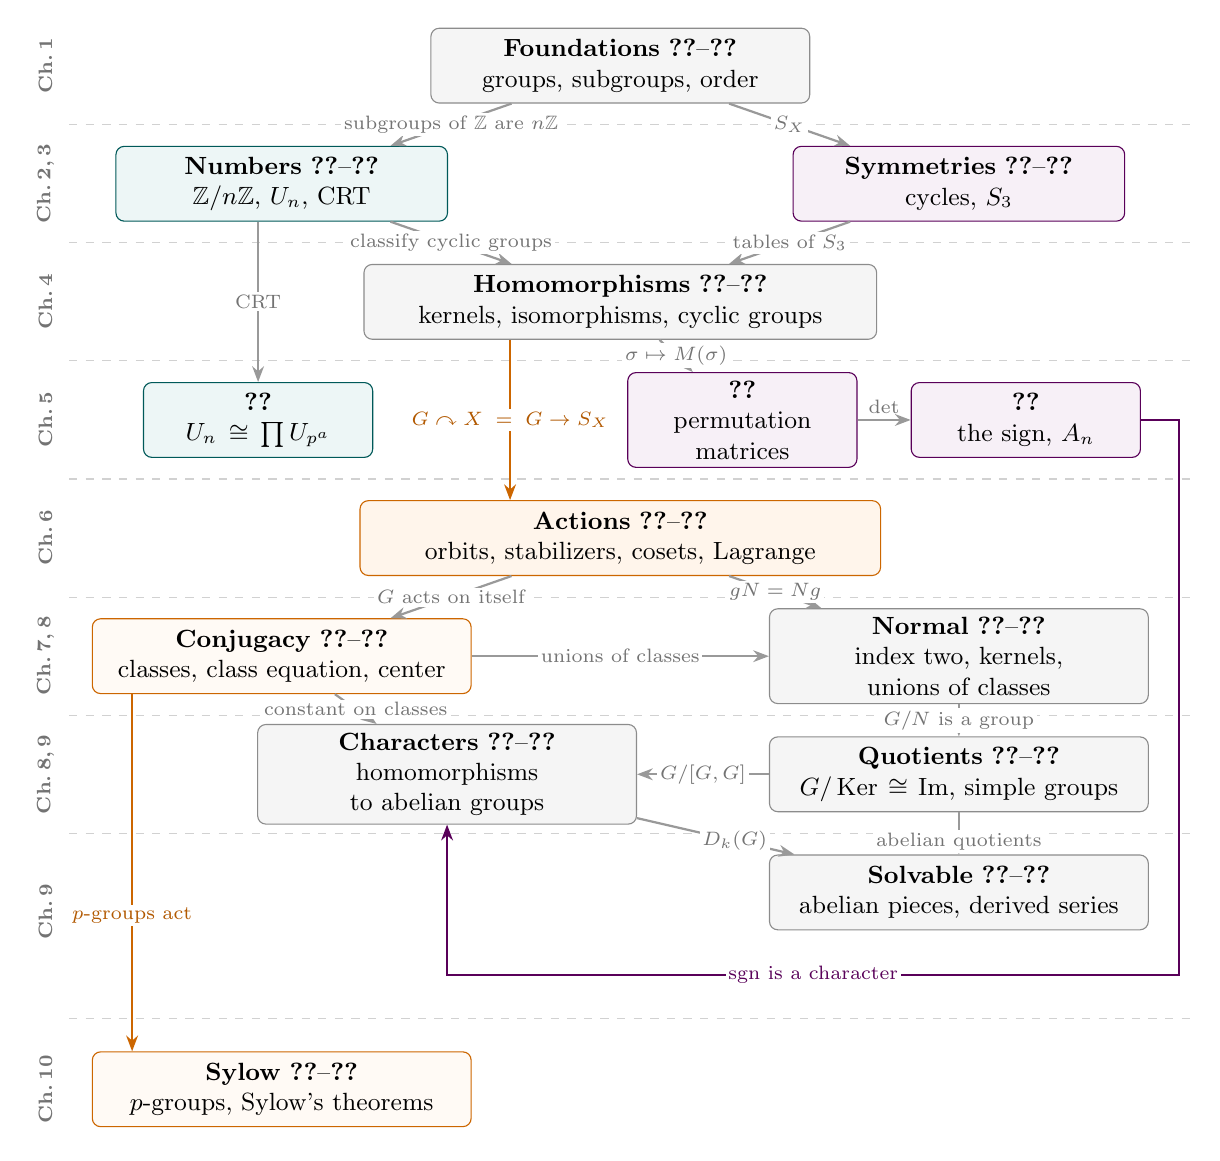
\begin{tikzpicture}[
    x=1cm, y=1cm, font=\small,
    box/.style={draw, rounded corners=3pt, align=center, inner sep=3pt, minimum height=0.95cm},
    shared/.style={box, draw=black!45, fill=black!4, text width=4.6cm},
    num/.style={box, draw=teal!70!black, fill=teal!7, text width=4.0cm},
    sym/.style={box, draw=violet!70!black, fill=violet!6, text width=4.0cm},
    act/.style={box, draw=orange!80!black, fill=orange!8, text width=6.4cm},
    small/.style={text width=2.7cm},
    link/.style={-{Stealth[length=2mm]}, draw=black!40, thick},
    bridge/.style={font=\scriptsize, text=black!55, fill=white, inner sep=1pt},
  ]
  \foreach \y/\t in {0/{Ch.\,1}, -1.5/{Ch.\,2,\,3}, -3.0/{Ch.\,4}, -4.5/{Ch.\,5}, -6.0/{Ch.\,6}, -7.5/{Ch.\,7,\,8}, -9.0/{Ch.\,8,\,9}, -10.75/{Ch.\,9}, -13.0/{Ch.\,10}}
    \node[rotate=90, font=\scriptsize\bfseries, text=black!55] at (-7.3,\y) {\t};
  \foreach \y in {-0.75,-2.25,-3.75,-5.25,-6.75,-8.25,-9.75,-12.1}
    \draw[black!18, dashed] (-7.0,\y) -- (7.25,\y);

  \node[shared] (found) at (0,0) {\textbf{Foundations} \ref*{sec:def-group}--\ref*{sec:zoo}\\ groups, subgroups, order};
  \node[num] (num) at (-4.3,-1.5) {\textbf{Numbers} \ref*{sec:divisibility}--\ref*{sec:crt}\\ $\mathbb{Z}/n\mathbb{Z}$, $U_n$, CRT};
  \node[sym] (sym) at (4.3,-1.5) {\textbf{Symmetries} \ref*{sec:cycles}--\ref*{sec:s3-subgroups}\\ cycles, $S_3$};
  \node[shared, text width=6.3cm] (hom) at (0,-3.0) {\textbf{Homomorphisms} \ref*{sec:tables}--\ref*{sec:conjugation-products}\\ kernels, isomorphisms, cyclic groups};
  \node[num, small] (un) at (-4.6,-4.5) {\ref*{sec:un-structure}\\ $U_n \cong \prod U_{p^a}$};
  \node[sym, small] (mat) at (1.55,-4.5) {\ref*{sec:actions}\\ permutation matrices};
  \node[sym, small] (sgn) at (5.15,-4.5) {\ref*{sec:sign}\\ the sign, $A_n$};
  \node[act] (act) at (0,-6.0) {\textbf{Actions} \ref*{sec:equivalence}--\ref*{sec:action-examples}\\ orbits, stabilizers, cosets, Lagrange};
  \node[box, draw=orange!80!black, fill=orange!4, text width=4.6cm] (conj) at (-4.3,-7.5) {\textbf{Conjugacy} \ref*{sec:conjugacy}--\ref*{sec:center}\\ classes, class equation, center};
  \node[shared] (norm) at (4.3,-7.5) {\textbf{Normal} \ref*{sec:multiplying-cosets}--\ref*{sec:normal-sources}\\ index two, kernels,\\ unions of classes};
  \node[shared] (quot) at (4.3,-9.0) {\textbf{Quotients} \ref*{sec:quotient}--\ref*{sec:simple}\\ $G/\operatorname{Ker} \cong \operatorname{Im}$, simple groups};
  \node[shared] (char) at (-2.2,-9.0) {\textbf{Characters} \ref*{sec:characters}--\ref*{sec:commutators}\\ homomorphisms to abelian groups};
  \node[shared] (solv) at (4.3,-10.5) {\textbf{Solvable} \ref*{sec:solvable}--\ref*{sec:rev-ch9}\\ abelian pieces, derived series};
  \node[box, draw=orange!80!black, fill=orange!4, text width=4.6cm] (syl) at (-4.3,-13.0) {\textbf{Sylow} \ref*{sec:p-groups}--\ref*{sec:sylow-theorems}\\ $p$-groups, Sylow's theorems};

  \draw[link] (found) -- node[bridge]{subgroups of $\mathbb{Z}$ are $n\mathbb{Z}$} (num);
  \draw[link] (found) -- node[bridge]{$S_X$} (sym);
  \draw[link] (num) -- node[bridge]{classify cyclic groups} (hom);
  \draw[link] (sym) -- node[bridge]{tables of $S_3$} (hom);
  \draw[link] ($(num.south)+(-0.3,0)$) -- node[bridge]{CRT} (un.north);
  \draw[link] (hom) -- node[bridge]{$\sigma \mapsto M(\sigma)$} (mat);
  \draw[link] (mat) -- node[bridge, above=1pt, fill=none]{$\det$} (sgn);
  \draw[link, draw=orange!80!black] ($(hom.south)+(-1.4,0)$) -- node[bridge, text=orange!70!black]{$G \curvearrowright X \;=\; G \to S_X$} ($(act.north)+(-1.4,0)$);
  \draw[link] (act) -- node[bridge]{$G$ acts on itself} (conj);
  \draw[link] (act) -- node[bridge]{$gN = Ng$} (norm);
  \draw[link] (conj) -- node[bridge]{unions of classes} (norm);
  \draw[link] (norm) -- node[bridge]{$G/N$ is a group} (quot);
  \draw[link] (quot) -- node[bridge]{$G/[G,G]$} (char);
  \draw[link] (conj) -- node[bridge]{constant on classes} (char);
  \draw[link, draw=violet!70!black] (sgn.east) -- (7.1,-4.5) -- (7.1,-11.55) -- node[bridge, text=violet!70!black]{$\sgn$ is a character} (-2.2,-11.55) -- (char.south);
  \draw[link] (quot) -- node[bridge, pos=0.7]{abelian quotients} (solv);
  \draw[link] (char) -- node[bridge, pos=0.62]{$D_k(G)$} (solv);
  \draw[link, draw=orange!80!black] ($(conj.south)+(-1.9,0)$) -- node[bridge, text=orange!70!black, pos=0.62]{$p$-groups act} ($(syl.north)+(-1.9,0)$);
\end{tikzpicture}
\end{center}

The labels on the arrows are the bridges. The classification of subgroups of $\mathbb{Z}$ (\ref{sec:zoo}) is what makes $\mathbb{Z}/n\mathbb{Z}$ the model finite group, and the Classification of Cyclic Groups (\ref{sec:cyclic}) shows every cyclic group is one of these. On the symmetries side, $\sigma \mapsto M(\sigma)$ (\ref{sec:actions}) turns permutations into matrices, and the determinant then gives the sign (\ref{sec:sign}). The central bridge is Actions Are Homomorphisms to $S_X$ (\ref{sec:action-def}): every construction below it --- cosets and Lagrange (\ref{sec:lagrange}), orbit--stabilizer (\ref{sec:orbit-stabilizer}), conjugacy classes and the class equation (\ref{sec:conjugation-action}) --- is an action in disguise. Normal subgroups are where the two lower branches meet: they are the unions of conjugacy classes (\ref{sec:normal-sources}) and exactly the subgroups for which coset multiplication is well defined (\ref{sec:multiplying-cosets}), which is what makes $G/N$ a group (\ref{sec:quotient}). Finally, characters are constant on conjugacy classes and kill commutators, so they factor through the abelianization $G/[G,G]$ (\ref{sec:commutators}); the sign, met on the symmetries thread, is the first nontrivial example. Chapter~9 then turns from the atoms to how they are assembled: solvable groups are those built from abelian pieces (the quotients $G_j/G_{j-1}$ of a chain), and the derived series $D_k(G)$ tests for them. Chapter~10 collects the Sylow theorems of Worksheet~10, on subgroups of prime-power order, ahead of the lecture.

\chapter*{Conventions and Notation}
\addcontentsline{toc}{chapter}{Conventions and Notation}
\markboth{Conventions and Notation}{Conventions and Notation}

{\renewcommand{\arraystretch}{1.3}
\begin{longtable}{p{4.2cm}p{10.3cm}}
\textbf{Symbol} & \textbf{Meaning} \\ \hline
$e$, \ $e_G$ & The identity element; the subscript names the group when several are in play ($\varphi(e_G) = e_H$). Worksheet 1 writes $1$. Exceptions by established convention: $0$ in additive groups, $[0]$ in $\mathbb{Z}/n\mathbb{Z}$, $[1]$ in $U_n$, $I_n$ for matrices, and the number $1$ in $k^\times$ and $\{\pm 1\}$. \\
$gh$, \ $g^{-1}$, \ $g^n$ & Product, inverse, integer power (\ref{sec:subgroups}). Additively: $g + h$, $-g$, $ng$. \\
$\langle g \rangle$, \ $\langle g_1, \ldots, g_k \rangle$ & Subgroup generated (\ref{sec:subgroups}). \\
$|G|$, \ $\operatorname{ord}(g)$ & Order of a group; order of an element (\ref{sec:order}). \\
$[G : H]$, \ $G/H$, \ $H\backslash G$ & Index; left cosets; right cosets (\ref{sec:cosets}, \ref{sec:lagrange}). \\
$S_X$, \ $S_n$ & Bijections of $X$; of $\{1, \ldots, n\}$. Composition is right-to-left: $(\sigma\tau)(i) = \sigma(\tau(i))$. \\
$(a_1\ a_2\ \cdots\ a_r)$ & Cycle notation (\ref{sec:cycles}). \\
$\sgn$, \ $A_n$ & Sign of a permutation and its kernel (\ref{sec:sign}). The problem sets write $\varepsilon$. \\
$GL_n(k)$, $SL_n(k)$, $O(n)$, $SO(n)$ & Linear groups (\ref{sec:examples}); $M(\sigma)$ is the permutation matrix (\ref{sec:actions}). \\
$\mathbb{Z}/n\mathbb{Z}$, \ $U_n$ & Integers modulo $n$; unit group $(\mathbb{Z}/n\mathbb{Z})^\times$ (\ref{sec:znz}, \ref{sec:units}). \\
$\varphi(n)$ & Euler's totient $|U_n|$. (Elsewhere $\varphi$ usually denotes a homomorphism; context decides.) \\
$\operatorname{Ker}\varphi$, \ $\operatorname{Im}\varphi$, \ $\cong$ & Kernel, image, isomorphism (\ref{sec:homs}, \ref{sec:isos}). \\
$c_a$, \ $\operatorname{Aut}(G)$ & Conjugation by $a$; automorphism group (\ref{sec:conjugation-products}). \\
$\operatorname{Conj}(g)$, \ $C_G(g)$, \ $Z(G)$ & Conjugacy class; centralizer (PS 3 writes $Z(g)$); center (\ref{sec:conjugacy}, \ref{sec:conjugation-action}, \ref{sec:center}). \\
$g \star x$, \ $G \curvearrowright X$, \ $X \curvearrowleft G$ & Action; left action; right action (\ref{sec:action-def}). \\
$\operatorname{Stab}(x)$, \ $\operatorname{Fix}(g)$, \ $Gx$ & Stabilizer, fixed points, orbit (\ref{sec:stabilizers}, \ref{sec:orbits}). \\
$G\backslash X$, \ $X/G$ & Orbit spaces of a left and a right action (\ref{sec:orbits}). \\
$H \trianglelefteq G$, \ $[G, G]$ & Normal subgroup (\ref{sec:normal}); commutator subgroup, also written $D(G)$ (\ref{sec:commutators}). \\
$D_k(G)$ & The $k$-th term of the derived series, $D_0(G) = G$, $D_{k+1}(G) = D(D_k(G))$ (\ref{sec:derived-series}). \\
$\#(G)$ & Worksheet 10's notation for $|G|$. \\
$G^{\mathrm{ab}}$ & Abelianization $G/[G,G]$ (\ref{sec:commutators}). \\
$G/N$, \ $\pi$ & Quotient group by a normal subgroup; canonical projection $g \mapsto gN$ (\ref{sec:quotient}). \\
$PSL_n(F)$ & Projective special linear group $SL_n(F)/Z$ (\ref{sec:simple}). \\
$HN$ & Product set $\{hn : h \in H,\ n \in N\}$ (\ref{sec:second-iso}). \\
$X \sqcup Y$ & Disjoint union: $X \cup Y$ with $X \cap Y = \varnothing$ (\ref{sec:representatives}). \\
$\hookrightarrow$, \ $\twoheadrightarrow$ & An injective map; a surjective map. \\
\textit{WS $k.m$}, \textit{PS $k.m$} & Provenance tags: Worksheet $k$ / Problem Set $k$, Problem $m$. \\
\end{longtable}}

\part{Group Theory}

\chapter{Groups and Subgroups}

% ============================================================================
% SECTION 1: GROUPS  (Worksheet 1)
% ============================================================================

\textit{Source: Worksheet 1 (Mon Aug 31).}

This chapter sets up the language used everywhere else: the group axioms and their first consequences (cancellation, uniqueness of the identity and of inverses); the examples that recur throughout --- $\mathbb{Z}$, $k^\times$, $S_X$, $GL_n(k)$, direct products; and subgroups, including the subgroup generated by one or several elements and the order of an element. It closes with Worksheet 1's survey of subgroups of $\mathbb{Z}$, $\mathbb{Z}^2$, $\mathbb{R}$ and $GL_2(\mathbb{R})$. Its one complete classification, that every subgroup of $\mathbb{Z}$ is $n\mathbb{Z}$, drives Chapter~\ref{ch:modn}.

\section{The Definition of a Group}\label{sec:def-group}

\textit{Reference: Pinter Ch.\ 2 (operations), Ch.\ 3 (the definition of groups).}

\begin{defbox}[Group]\label{def:group}
A \textbf{group} $G$ is a set with a binary operation $*: G \times G \to G$ obeying the properties:
\begin{enumerate}
    \item \textbf{(Identity)} There is an element $e \in G$ such that $e * g = g * e = g$ for all $g \in G$.
    \item \textbf{(Inverses)} For all $g \in G$, there is an element $g^{-1}$ obeying $g * g^{-1} = g^{-1} * g = e$.
    \item \textbf{(Associativity)} For all $g_1, g_2, g_3 \in G$, we have $(g_1 * g_2) * g_3 = g_1 * (g_2 * g_3)$.
\end{enumerate}
\end{defbox}

\begin{defbox}[Abelian Group]\label{def:abelian-group}
A group $G$ is \textbf{abelian} (or \textbf{commutative}) if $a * b = b * a$ for all $a, b \in G$. Commutativity is \emph{not} one of the group axioms; groups such as $S_n$ ($n \geq 3$) and $GL_n(k)$ ($n \geq 2$) are non-abelian.
\end{defbox}

\begin{rembox}[Notation]\label{rem:notation}
Depending on context, we may denote $*$ by $*$, $\times$, $\cdot$, or no symbol at all, and the identity has been written $1$ (Worksheet 1), $e$ (lectures), or $\operatorname{Id}$. These notes write $e$, and $e_G$, $e_H$, \ldots\ whenever more than one group is in play. When the operation is written additively ($+$), the identity is written $0$ and the inverse of $g$ is written $-g$. Additive notation is used only for abelian groups (Worksheet 3: ``we never use these notations for a non-abelian group''), so the symbol $+$ itself signals commutativity.
\end{rembox}

\begin{propbox}[Generalized Associativity]\label{prop:generalized-associativity}
For any $g_1, \ldots, g_n \in G$, all ways of parenthesizing the product $g_1 * g_2 * \cdots * g_n$ give the same element. Consequently parentheses may be omitted from products, as they are from now on.
\end{propbox}

\begin{proof}
Let $L_n = (\cdots((g_1g_2)g_3)\cdots)g_n$ be the left-normed product; we show by induction on $n$ that every parenthesization equals $L_n$. The cases $n \leq 2$ are trivial. For $n \geq 3$, any parenthesization has an outermost multiplication $A \cdot B$, where $A$ is a parenthesization of $g_1 \cdots g_j$ and $B$ of $g_{j+1} \cdots g_n$ for some $1 \leq j < n$. By induction $A = L_j$ and $B$ equals the left-normed product of $g_{j+1}, \ldots, g_n$. If $j = n - 1$, then $B = g_n$ and $AB = L_{n-1}g_n = L_n$. If $j < n - 1$, write $B = B'g_n$ with $B'$ the left-normed product of $g_{j+1}, \ldots, g_{n-1}$; then $AB = A(B'g_n) = (AB')g_n$ by axiom (3), and $AB'$ is a parenthesization of $g_1 \cdots g_{n-1}$, hence equals $L_{n-1}$ by induction. So $AB = L_{n-1}g_n = L_n$.
\end{proof}

\begin{rembox}[Comparison with MATH 590]\label{rem:comparison-math-590}
This is the same definition as in the algebra-prerequisites section of the topology notes (590 notes, \S 17), with the axioms listed in a different order. WS 1.1--1.4 below establish the basic uniqueness and cancellation facts, which appeared as remarks in the 590 notes.
\end{rembox}

\section{First Consequences of the Axioms (WS 1.1--1.4)}\label{sec:consequences}

\textit{Reference: Pinter Ch.\ 4, Thms.\ 1--3.}

\begin{propbox}[{Cancellation, and What the Mixed Hypothesis Really Gives (WS 1.1)}]\label{prop:cancellation-what-mixed-hypothesis-really-gives}
Let $g, h_1, h_2 \in G$.
\begin{enumerate}
    \item \textbf{(Left cancellation)} If $g h_1 = g h_2$, then $h_1 = h_2$. (Likewise, $h_1 g = h_2 g$ implies $h_1 = h_2$: \textbf{right cancellation}.)
    \item \textbf{(Mixed hypothesis --- the worksheet's second part)} If $g h_1 = h_2 g$, then $h_2 = g h_1 g^{-1}$. In general this does \emph{not} force $h_1 = h_2$ (see the example The Mixed Hypothesis Does Not Cancel, below); rather, $h_1 = h_2$ holds if and only if $g h_1 = h_1 g$, i.e.\ iff $g$ and $h_1$ commute.
\end{enumerate}
\end{propbox}

\begin{proof}
\textbf{(1)} Suppose $g h_1 = g h_2$. Multiply both sides on the left by $g^{-1}$, which exists by axiom (2):
\[ g^{-1} (g h_1) = g^{-1} (g h_2). \]
By associativity (axiom (3)), $(g^{-1} g) h_1 = (g^{-1} g) h_2$, so by axiom (2), $e \cdot h_1 = e \cdot h_2$, and by axiom (1), $h_1 = h_2$.

For right cancellation, suppose $h_1 g = h_2 g$. Multiplying both sides on the \emph{right} by $g^{-1}$ and applying axioms (3), (2), (1) in the same order:
\[ h_1 = h_1 (g g^{-1}) = (h_1 g) g^{-1} = (h_2 g) g^{-1} = h_2 (g g^{-1}) = h_2.
\]

\textbf{(2)} Suppose $g h_1 = h_2 g$. Multiplying both sides on the \emph{right} by $g^{-1}$:
\[ g h_1 g^{-1} = h_2 (g g^{-1}) = h_2. \]
Now, if $h_1 = h_2$, substituting into the hypothesis gives $g h_1 = h_1 g$. Conversely, if $g h_1 = h_1 g$, then $h_2 = g h_1 g^{-1} = h_1 (g g^{-1}) = h_1$. So under the mixed hypothesis, $h_1 = h_2 \iff g h_1 = h_1 g$.
\end{proof}

\begin{exbox}[{The Mixed Hypothesis Does Not Cancel (WS 1.1)}]\label{ex:mixed-hypothesis-does-not-cancel}
In $S_3$, take $g = (1\,2)$, $h_1 = (2\,3)$, $h_2 = (1\,3)$. Computing (right factor first):
\[ g h_1 = (1\,2)(2\,3) = (1\,2\,3), \qquad h_2 g = (1\,3)(1\,2) = (1\,2\,3), \]
so $g h_1 = h_2 g$ --- yet $h_1 = (2\,3) \neq (1\,3) = h_2$. Consistently with part (2), $h_2 = g h_1 g^{-1}$: conjugating the swap $2 \leftrightarrow 3$ by the relabeling $1 \leftrightarrow 2$ produces the swap $1 \leftrightarrow 3$.
\end{exbox}

\begin{rembox}[{Left vs.\ Right; Conjugation}]\label{rem:left-vs-right-conjugation}
The moral of part (2): in a non-abelian group, ``multiply both sides by $g^{-1}$'' is only valid on the \emph{same side} of both expressions; multiplying on opposite sides transports an element to its \emph{conjugate} $g h g^{-1}$ instead of cancelling it. In an abelian group the mixed hypothesis \emph{does} give $h_1 = h_2$. Conjugation --- and the way conjugating a permutation ``relabels'' the objects it moves, as in The Mixed Hypothesis Does Not Cancel --- will become a central tool later (normal subgroups, conjugacy classes).
\end{rembox}

\begin{propbox}[{Uniqueness of the Identity (WS 1.2)}]\label{prop:uniqueness-identity}
$G$ contains exactly one element $e$ obeying condition (1) of the definition of a group.
\end{propbox}

\begin{proof}
Suppose $e$ and $e'$ both obey condition (1). Evaluate the single product $e * e'$ in two ways. Since $e'$ satisfies (1) (with $g = e$): $e * e' = e$. Since $e$ satisfies (1) (with $g = e'$): $e * e' = e'$. Hence $e = e * e' = e'$.
\end{proof}

\begin{propbox}[{Uniqueness of Inverses (WS 1.3)}]\label{prop:uniqueness-inverses}
For each $g \in G$, there is exactly one element $g^{-1} \in G$ obeying condition (2) of the definition of a group.
\end{propbox}

\begin{proof}
Suppose $h$ and $h'$ both obey condition (2) for $g$, i.e.\ $g h = h g = e$ and $g h' = h' g = e$. Then $g h = e = g h'$, so by left cancellation (Cancellation, \ref{sec:consequences}), $h = h'$.

\textit{Alternative direct computation (avoiding WS 1.1):}
\[ h = h \cdot e = h (g h') = (h g) h' = e \cdot h' = h'. \]
\end{proof}

\begin{rembox}[The Uniqueness Technique]\label{rem:uniqueness-technique}
WS 1.3 gives the standard technique for computing inverses: since the inverse of $x$ is \emph{unique}, to prove $y = x^{-1}$ it suffices to verify that $y$ satisfies the defining property $x y = y x = e$. WS 1.4 and 1.5 below, and the identity $(AB)^{-1} = B^{-1} A^{-1}$ for matrices, are all proved this way. (Compare the 590 notes, where the same pattern proves bijectivity via a two-sided inverse.)
\end{rembox}

\begin{propbox}[{Inverse of a Product (WS 1.4)}]\label{prop:inverse-product}
For all $g, h \in G$: \ $(gh)^{-1} = h^{-1} g^{-1}$.
\end{propbox}

\begin{proof}
By WS 1.3, it suffices to verify that $h^{-1} g^{-1}$ satisfies the defining property of the inverse of $gh$:
\[ (gh)(h^{-1} g^{-1}) = g (h h^{-1}) g^{-1} = g \cdot e \cdot g^{-1} = g g^{-1} = e, \]
\[ (h^{-1} g^{-1})(gh) = h^{-1} (g^{-1} g) h = h^{-1} \cdot e \cdot h = h^{-1} h = e. \]
Since the inverse of $gh$ is unique and $h^{-1}g^{-1}$ satisfies its defining property, $(gh)^{-1} = h^{-1} g^{-1}$.
\end{proof}

\begin{corbox}[{Inverse of a Product of $n$ Elements}]\label{cor:inverse-product-n-elements}
For $g_1, \ldots, g_n \in G$: \ $(g_1 g_2 \cdots g_n)^{-1} = g_n^{-1} \cdots g_2^{-1} g_1^{-1}$.
\end{corbox}

\begin{proof}
Induct on $n$, the case $n = 2$ being the proposition: $(g_1 \cdots g_n)^{-1} = \big((g_1 \cdots g_{n-1})g_n\big)^{-1} = g_n^{-1}(g_1 \cdots g_{n-1})^{-1} = g_n^{-1}g_{n-1}^{-1} \cdots g_1^{-1}$.
\end{proof}

\begin{rembox}[Socks and Shoes]\label{rem:socks-shoes}
The order reversal is forced in non-abelian groups: to undo ``put on socks, then shoes,'' remove shoes first.
\end{rembox}

\begin{propbox}[{One-Sided Inverses Suffice (cf.\ Pinter Ch.\ 4, Thm.\ 2--3)}]\label{prop:one-sided-inverses-suffice}
Let $a, b \in G$.
\begin{enumerate}
    \item If $ab = e$, then $b = a^{-1}$ and $a = b^{-1}$. Consequently $ab = e$ implies $ba = e$.
    \item $(a^{-1})^{-1} = a$.
\end{enumerate}
\end{propbox}

\begin{proof}
\textbf{(1)} If $ab = e$, then $ab = a a^{-1}$, so $b = a^{-1}$ by left cancellation (Cancellation, \ref{sec:consequences}). Likewise $ab = e = b^{-1} b$ gives $a = b^{-1}$ by right cancellation. Then $ba = a^{-1} a = e$.

\textbf{(2)} The element $a$ satisfies $a^{-1} a = a a^{-1} = e$, which is the defining property of the inverse of $a^{-1}$; by uniqueness of inverses (Uniqueness of Inverses, \ref{sec:consequences}), $(a^{-1})^{-1} = a$.
\end{proof}

\begin{rembox}[Why One-Sided Suffices Here but Not in General]\label{rem:why-one-sided-suffices-here-but-not-general}
In a group, checking $ab = e$ alone certifies $b = a^{-1}$; the other equation $ba = e$ comes free. This is special to groups (it uses that $a$ already \emph{has} a two-sided inverse). In monoids --- e.g.\ functions $X \to X$ under composition for infinite $X$ --- a one-sided inverse need not be two-sided: the shift $n \mapsto n + 1$ on $\mathbb{N}$ has a left inverse but no right inverse.
\end{rembox}

\begin{propbox}[{Unique Solvability of Linear Equations (cf.\ Pinter Ch.\ 4)}]\label{prop:unique-solvability-linear-equations}
Let $a, b \in G$. The equation $ax = b$ has exactly one solution $x \in G$, namely $x = a^{-1} b$; and $xa = b$ has exactly one solution, namely $x = b a^{-1}$.
\end{propbox}

\begin{proof}
\textbf{Existence:} $a(a^{-1} b) = (a a^{-1}) b = b$. \textbf{Uniqueness:} if $ax = b = ax'$, then $x = x'$ by left cancellation. The equation $xa = b$ is handled symmetrically with right cancellation.
\end{proof}

\begin{corbox}[Latin Square Property]\label{cor:latin-square-property}
In the multiplication table of a finite group, every element appears exactly once in each row and exactly once in each column; that is, the table is a \emph{Latin square}.
\end{corbox}

\begin{proof}
In the row of $a$, the element $b$ appears in column $x$ iff $ax = b$, and by Unique Solvability this has exactly one solution: existence gives ``at least once,'' uniqueness (cancellation) ``at most once.'' Columns are handled the same way with $xa = b$.
\end{proof}

\begin{rembox}[The Converse Fails]\label{rem:converse-fails}
A Latin square need not be a group table, since associativity is not encoded row by row. The property is visible in the $S_3$ table (\ref{sec:cycles}).
\end{rembox}

\section{Basic Examples of Groups}\label{sec:examples}

\textit{Reference: Pinter Ch.\ 3 (examples of groups), Ch.\ 7 (groups of permutations), Ch.\ 4, Ex.\ G (direct products).}

In each example, associativity is inherited from a known associative operation (arithmetic, function composition); the nontrivial points are \emph{well-definedness} (for $\mathbb{Z}/n\mathbb{Z}$ and $U_n$) and \emph{closure} (for $U_n$, $S_X$, $GL_n$).

\begin{defbox}[{The Additive Groups $\mathbb{Z}$, $\mathbb{Q}$, $\mathbb{R}$}]\label{def:additive-groups-z-q-r}
Each of $\mathbb{Z}$, $\mathbb{Q}$, $\mathbb{R}$ is a group under addition: the operation is $(a, b) \mapsto a + b$ (which lands in the same set, so closure holds); the identity is $0$; the inverse of $a$ is $-a$. Associativity is a basic property of arithmetic. All three are abelian. \textit{(Note: none of them is a group under multiplication --- $0$ has no inverse, and in $\mathbb{Z}$ even $2$ has no inverse.)}
\end{defbox}

\begin{defbox}[Direct Products]\label{def:direct-products}
Let $G$ and $H$ be groups. The \textbf{direct product} $G \times H$ is the set of pairs $\{(g, h) : g \in G, h \in H\}$ with componentwise operation
\[ (g_1, h_1) * (g_2, h_2) = (g_1 g_2, h_1 h_2). \]
This is a group: identity $(e_G, e_H)$, inverse $(g, h)^{-1} = (g^{-1}, h^{-1})$, and each axiom holds componentwise because it holds in $G$ and in $H$. Iterating gives $G_1 \times \cdots \times G_n$; in particular $\mathbb{Z}^n$, $\mathbb{Q}^n$, $\mathbb{R}^n$ (componentwise addition, identity $(0, \ldots, 0)$) and mixed products like $\mathbb{Z} \times \mathbb{R}$.
\end{defbox}

\begin{defbox}[Field (provisional definition)]\label{def:field-provisional-definition}
A \textbf{field} is a set $k$ with two operations $+$ and $\cdot$ such that:
\begin{enumerate}
    \item $(k, +)$ is an abelian group, with identity written $0$;
    \item $(k \setminus \{0\}, \cdot)$ is an abelian group, with identity written $1$;
    \item multiplication distributes over addition: $a(b + c) = ab + ac$ for all $a, b, c \in k$.
\end{enumerate}
Examples: $\mathbb{Q}$, $\mathbb{R}$, $\mathbb{C}$; also $\mathbb{Z}/p\mathbb{Z}$ for $p$ prime (see the unit-group discussion below). Non-examples: $\mathbb{Z}$ (no multiplicative inverses). Fields will be treated properly later in the course; this definition suffices for now.
\end{defbox}

\begin{defbox}[{Multiplicative Group of a Field: $k^\times$}]\label{def:multiplicative-group-field-k-x}
For a field $k$, set $k^\times = (k \setminus \{0\}, \cdot)$; this is a group directly by condition (2) of the field definition, e.g.\ $\mathbb{Q}^\times$, $\mathbb{R}^\times$, $\mathbb{C}^\times$.
\end{defbox}

\begin{propbox}[No Zero Divisors in a Field]\label{prop:no-zero-divisors-field}
Let $k$ be a field. Then $a \cdot 0 = 0$ for every $a \in k$, and if $ab = 0$ then $a = 0$ or $b = 0$. In particular the product of two nonzero elements is nonzero.
\end{propbox}

\begin{proof}
$a \cdot 0 = a(0 + 0) = a \cdot 0 + a \cdot 0$, and cancelling $a \cdot 0$ in the group $(k, +)$ gives $a \cdot 0 = 0$. If $ab = 0$ and $a \neq 0$, then $b = 1 \cdot b = (a^{-1}a)b = a^{-1}(ab) = a^{-1} \cdot 0 = 0$.
\end{proof}

\begin{rembox}[Consistency of the Field Axioms]\label{rem:consistency-field-axioms}
With the definition of a field above, closure of $k \setminus \{0\}$ under multiplication is built into condition (2) ($\cdot$ is a binary operation \emph{on} $k \setminus \{0\}$); the proposition shows this is consistent with the remaining axioms rather than an extra assumption in disguise.
\end{rembox}

\begin{defbox}[{Symmetric Groups $S_X$ and $S_n$}]\label{def:symmetric-groups-sx-sn}
For any set $X$, let $S_X$ be the set of bijections $\sigma: X \to X$, with operation composition: $(\sigma \tau)(x) = \sigma(\tau(x))$ (\textbf{convention:} apply the right factor first). Then $S_X$ is a group with identity $\operatorname{id}_X$ and inverse the inverse function $\sigma^{-1}$. If $X = \{1, 2, \ldots, n\}$, we call this group the \textbf{symmetric group} and denote it $S_n$; it has $n!$ elements and is non-abelian for $n \geq 3$.
\end{defbox}

\begin{proof}[Verification]
\textbf{Closure:} A composition of bijections is a bijection: if $\sigma, \tau$ have inverse functions $\sigma^{-1}, \tau^{-1}$, then $\tau^{-1} \sigma^{-1}$ is a two-sided inverse of $\sigma\tau$ (note the socks--shoes reversal, exactly WS 1.4), and a function with a two-sided inverse is a bijection.

\textbf{Associativity:} Function composition is associative: for every $x$,
\[ ((\sigma\tau)\rho)(x) = (\sigma\tau)(\rho(x)) = \sigma(\tau(\rho(x))) = \sigma((\tau\rho)(x)) = (\sigma(\tau\rho))(x). \]

\textbf{Identity and inverses:} $\operatorname{id}_X \circ \sigma = \sigma \circ \operatorname{id}_X = \sigma$, and the inverse \emph{function} $\sigma^{-1}$ (which exists precisely because $\sigma$ is a bijection) satisfies $\sigma \sigma^{-1} = \sigma^{-1} \sigma = \operatorname{id}_X$.

\textbf{Non-abelian for $n \geq 3$:} With $g_1 = (1\,2)$, $g_2 = (2\,3)$: $g_1 g_2$ sends $1 \to 2$, while $g_2 g_1$ sends $1 \to 3$ (see The Group $S_3$ in Detail, \ref{sec:cycles}).

\textbf{Order:} A bijection of $\{1, \ldots, n\}$ is determined by choosing $\sigma(1)$ ($n$ ways), then $\sigma(2)$ ($n - 1$ remaining values), etc., giving $n!$.
\end{proof}

\begin{defbox}[{General Linear Groups $GL_n(k)$}]\label{def:general-linear-groups-gln-k}
For a field $k$ and integer $n \geq 1$, let
\[ GL_n(k) = \{ A \in \operatorname{Mat}_{n \times n}(k) : A \text{ is invertible} \}, \]
with operation matrix multiplication. Then $GL_n(k)$ is a group with identity the identity matrix $I_n$ and inverse the matrix inverse $A^{-1}$, called the \textbf{general linear group}. It is non-abelian for $n \geq 2$.
\end{defbox}

\begin{proof}[Verification]
\textbf{Closure:} If $A, B$ are invertible, then $B^{-1}A^{-1}$ is a two-sided inverse of $AB$ (WS 1.4 again: $(AB)(B^{-1}A^{-1}) = A(BB^{-1})A^{-1} = I_n$ and symmetrically), so $AB \in GL_n(k)$. \textit{(Equivalently, once determinants are available: $A$ is invertible iff $\det A \neq 0$, and $\det(AB) = \det A \det B \neq 0$.)}

\textbf{Associativity:} Matrix multiplication is associative --- either by direct computation with the entry formula $\left( (AB)C \right)_{il} = \sum_{j,\,m} A_{ij} B_{jm} C_{ml} = \left( A(BC) \right)_{il}$ (both orders of summation give the same double sum), or conceptually: matrices represent linear maps $k^n \to k^n$, matrix multiplication represents composition, and composition of functions is associative (as verified for $S_X$).

\textbf{Identity and inverses:} $I_n A = A I_n = A$, and $A^{-1} \in GL_n(k)$ since $A^{-1}$ has the two-sided inverse $A$.

\textbf{Non-abelian for $n \geq 2$:}
$\begin{pmatrix} 1 & 1 \\ 0 & 1 \end{pmatrix}\begin{pmatrix} 1 & 0 \\ 1 & 1 \end{pmatrix} = \begin{pmatrix} 2 & 1 \\ 1 & 1 \end{pmatrix}$ but
$\begin{pmatrix} 1 & 0 \\ 1 & 1 \end{pmatrix}\begin{pmatrix} 1 & 1 \\ 0 & 1 \end{pmatrix} = \begin{pmatrix} 1 & 1 \\ 1 & 2 \end{pmatrix}$
(in any field where $2 \neq 0$ these differ in the $(1,1)$ entry; over $\mathbb{F}_2$ they still differ in the off-diagonal entries).
\end{proof}

\begin{defbox}[{Special Linear Group}]\label{def:special-linear-orthogonal-special-orthogonal}
For a field $k$ and $n \geq 1$, the \textbf{special linear group} is $SL_n(k) = \{A \in GL_n(k) : \det A = 1\}$.
\end{defbox}

\begin{defbox}[{Orthogonal Group}]\label{def:orthogonal-group}
For $n \geq 1$, the \textbf{orthogonal group} is $O(n) = O_n(\mathbb{R}) = \{A \in GL_n(\mathbb{R}) : A^{\mathsf{T}}A = I_n\}$.
\end{defbox}

\begin{defbox}[{Special Orthogonal Group}]\label{def:special-orthogonal-group}
The \textbf{special orthogonal group} is $SO(n) = O(n) \cap SL_n(\mathbb{R})$.
\end{defbox}

Each of $SL_n(k)$, $O(n)$ and $SO(n)$ is a subgroup of the corresponding general linear group (verified in \ref{sec:zoo}, where $SO(2)$ is identified with the rotations of the plane).

\begin{exbox}[{Groups and Non-Groups (cf.\ MATH 412)}]\label{ex:groups-non-groups}
Deciding whether $(G, \cdot)$ is a group usually comes down to identity and inverses; associativity is inherited from arithmetic or composition.
\begin{center}
\begin{tabular}{lll}
$(\mathbb{N}, +)$: no (no inverses) & $(\mathbb{N}, \times)$: no & $(\mathbb{Z}, +)$: yes \\
$(\mathbb{Z}, \times)$: no ($2$ has no inverse) & $(\mathbb{R}_{\geq 0}, +)$: no & $(\mathbb{R}, +)$: yes \\
$(\mathbb{R}_{\geq 0}, \times)$: no ($0$) & $(\mathbb{R}, \times)$: no ($0$) & $(\mathbb{R}\setminus\{0\}, \times)$: yes \\
$(\mathbb{Z}/n\mathbb{Z}, +)$: yes & $(\mathbb{Z}/n\mathbb{Z}, \times)$: no ($[0]$) & $(\mathbb{Z}/n\mathbb{Z} \setminus \{[0]\}, \times)$: iff $n$ prime \\
$(GL_n(\mathbb{R}), \times)$: yes & $(SL_n(\mathbb{R}), \times)$: yes & $(\mathbb{R}_{>0}, \times)$: yes
\end{tabular}
\end{center}
\end{exbox}

\begin{rembox}[{$S_n$ and $GL_n(k)$}]\label{rem:sn-gln-k}
$S_n$ and $GL_n(k)$ are the two fundamental families of non-abelian groups. $S_n$ acts by permuting a finite set; $GL_n(k)$ acts linearly on a vector space. Representation theory (second half of the course) is precisely the study of homomorphisms $G \to GL_n(k)$, i.e.\ of realizing abstract groups inside the second family.
\end{rembox}

\section{Subgroups}\label{sec:subgroups}

\textit{Reference: Pinter Ch.\ 5 (subgroups), Ch.\ 10 (order of group elements), Ch.\ 11 (cyclic groups).}

\begin{defbox}[Subgroup]\label{def:subgroup}
Let $G$ be a group and let $H$ be a subset of $G$. We say that $H$ is a \textbf{subgroup} of $G$ if
\begin{enumerate}
    \item $e_G \in H$;
    \item if $h \in H$, then $h^{-1} \in H$;
    \item if $h_1$ and $h_2 \in H$, then $h_1 h_2 \in H$.
\end{enumerate}
So a subgroup of $G$ is itself a group, with the same identity and inverse map.
\end{defbox}

\begin{propbox}[A Subset That Is a Group Is a Subgroup]\label{prop:subset-group-subgroup}
A subgroup of $G$ is a group under the restricted operation, with the same identity and inverse map. Conversely, let $H \subseteq G$ be closed under the operation of $G$ and suppose $H$ is a group under the restricted operation. Then the identity of $H$ is $e_G$ and inverses in $H$ are inverses in $G$; hence $H$ is a subgroup of $G$.
\end{propbox}

\begin{proof}
For a subgroup, condition (3) makes the restriction of $*$ a binary operation on $H$, associativity is inherited, and conditions (1) and (2) supply identity and inverses. Conversely, let $e$ be the identity of $H$. Then $e * e = e = e * e_G$ in $G$, and cancelling $e$ on the left (Cancellation) gives $e = e_G$. For $h \in H$, its inverse $h'$ in $H$ satisfies $hh' = h'h = e = e_G$, so $h'$ is an inverse of $h$ in $G$, and $h' = h^{-1}$ by Uniqueness of Inverses.
\end{proof}

\begin{propbox}[{Equivalent Subgroup Criteria (cf.\ Pinter Ch.\ 5)}]\label{prop:equivalent-subgroup-criteria}
Let $H$ be a subset of a group $G$. The following are equivalent:
\begin{enumerate}
    \item $H$ is a subgroup: $e \in H$, and $H$ is closed under inverses and under products.
    \item $H$ is \emph{nonempty}, and $H$ is closed under inverses and under products.
    \item $H$ is nonempty, and $a, b \in H$ implies $a b^{-1} \in H$ (the \textbf{one-step test}).
\end{enumerate}
\end{propbox}

\begin{proof}
(1) $\Rightarrow$ (2): $e \in H$ makes $H$ nonempty. (2) $\Rightarrow$ (3): given $a, b \in H$, $b^{-1} \in H$ by closure under inverses, then $ab^{-1} \in H$ by closure under products. (3) $\Rightarrow$ (1): pick any $a \in H$ (nonempty); then $e = a a^{-1} \in H$. For $b \in H$, $b^{-1} = e \cdot b^{-1} \in H$. For $a, b \in H$, we now know $b^{-1} \in H$, so $ab = a (b^{-1})^{-1} \in H$, using $(b^{-1})^{-1} = b$.
\end{proof}

\begin{propbox}[{Intersections of Subgroups (cf.\ Pinter Ch.\ 5, Ex.\ D1)}]\label{prop:intersections-subgroups}
If $\{H_i\}_{i \in I}$ is any nonempty family of subgroups of $G$, then $\bigcap_{i \in I} H_i$ is a subgroup of $G$. (Unions are \emph{not} subgroups in general: $2\mathbb{Z} \cup 3\mathbb{Z}$ contains $2$ and $3$ but not $5$.)
\end{propbox}

\begin{proof}
Let $K = \bigcap_i H_i$. Since $e \in H_i$ for every $i$, $e \in K$. If $h \in K$, then $h \in H_i$ for every $i$, so $h^{-1} \in H_i$ for every $i$, so $h^{-1} \in K$. If $h_1, h_2 \in K$, then $h_1, h_2 \in H_i$ for every $i$, so $h_1 h_2 \in H_i$ for every $i$, so $h_1 h_2 \in K$. Each condition is checked ``coordinatewise in $i$'' and survives the intersection.
\end{proof}

\subsection{Integer Powers and the Subgroup Generated by One Element}

\begin{defbox}[{Integer Powers (lecture 9/9)}]\label{def:integer-powers}
Let $G$ be a group and $g \in G$. Define $g^0 = e$; for $n \geq 1$, define inductively $g^n = g^{n-1} g$ (unambiguous by generalized associativity); and for $n \geq 1$, define $g^{-n} = (g^{-1})^n$. (By law (1) below this equals $(g^n)^{-1}$, the form used in lecture.)
\end{defbox}

\begin{lembox}[{Exponent Laws (lecture 9/9; cf.\ Pinter Ch.\ 10, Thm.\ 1)}]\label{lem:exponent-laws}
For all $g \in G$ and all $m, n \in \mathbb{Z}$:
\begin{enumerate}
    \item $(g^n)^{-1} = g^{-n}$;
    \item $g^m g^n = g^{m+n}$;
    \item $(g^m)^n = g^{mn}$.
\end{enumerate}
\end{lembox}

\begin{proof}
\textbf{Step 0 ($g$ commutes with its own powers):} For $n \geq 0$, $g \, g^n = g^n g$, by induction: trivial for $n = 0$; and $g \, g^{n+1} = g (g^n g) = (g \, g^n) g = (g^n g) g = g^{n+1} g$.

\textbf{Step 1 (law (2) for $m, n \geq 0$):} Induct on $n$. For $n = 0$: $g^m g^0 = g^m$. Assuming $g^m g^n = g^{m+n}$:
\[ g^m g^{n+1} = g^m (g^n g) = (g^m g^n) g = g^{m+n} g = g^{m+n+1}. \]

\textbf{Step 2 (law (1) for $n \geq 0$):} Induct on $n$. For $n = 0$: $(g^0)^{-1} = e^{-1} = e = g^{0}$. Assuming $(g^n)^{-1} = (g^{-1})^n$:
\[ (g^{n+1})^{-1} = (g^n g)^{-1} \overset{\text{Prob.\ 1.4}}{=} g^{-1} (g^n)^{-1} = g^{-1} (g^{-1})^n \overset{\text{Step 0 for } g^{-1}}{=} (g^{-1})^n g^{-1} = (g^{-1})^{n+1} = g^{-(n+1)}. \]
For $n < 0$, write $n = -p$ with $p > 0$: $(g^{-p})^{-1} = ((g^{-1})^p)^{-1} = ((g^{-1})^{-1})^p = g^p$, using the $\geq 0$ case applied to $g^{-1}$ and $(g^{-1})^{-1} = g$ (which holds since $g$ satisfies the defining property of the inverse of $g^{-1}$, and inverses are unique by WS 1.3).

\textbf{Step 3 (law (2), mixed signs):} If $m, n \leq 0$, apply Step 1 to $g^{-1}$: $g^m g^n = (g^{-1})^{-m}(g^{-1})^{-n} = (g^{-1})^{-m-n} = g^{m+n}$. Now suppose $m \geq 0 \geq n$.

\textit{Subcase $m + n \geq 0$:} Step 1 (both exponents $\geq 0$) gives $g^{m+n} g^{-n} = g^m$. Multiplying on the right by $g^n = (g^{-n})^{-1}$ (Step 2) yields $g^{m+n} = g^m g^n$.

\textit{Subcase $m + n < 0$:} Write $-n = m + r$ with $r = -(m+n) > 0$. By Step 1 applied to $g^{-1}$: $g^n = (g^{-1})^{-n} = (g^{-1})^{m} (g^{-1})^{r}$. Hence, using $(g^{-1})^m = (g^m)^{-1}$ (Step 2):
\[ g^m g^n = g^m (g^m)^{-1} (g^{-1})^r = (g^{-1})^r = g^{-r} = g^{m+n}. \]
The remaining case $n \geq 0 \geq m$ follows by the mirror-image argument (multiply on the left instead of the right).

\textbf{Step 4 (law (3)):} First let $n \geq 0$ and induct on $n$: for $n = 0$, $(g^m)^0 = e = g^0$. Assuming $(g^m)^n = g^{mn}$,
\[ (g^m)^{n+1} = (g^m)^n g^m = g^{mn} g^m \overset{(2)}{=} g^{mn + m} = g^{m(n+1)}. \]
For $n < 0$, write $n = -p$ with $p > 0$: $(g^m)^{-p} = \big((g^m)^p\big)^{-1} \overset{(1)}{=} (g^{mp})^{-1} \overset{(1)}{=} g^{-mp} = g^{mn}$, using the definition of negative powers and law (1) applied to the element $g^m$ and then to $g$.
\end{proof}

\begin{rembox}[Two Non-Laws]\label{rem:two-non-laws}
The exponent laws concern powers of a \emph{single} element. For two elements, as stressed in lecture:
\[ (gh)^2 = ghgh, \text{ which is ``probably not'' } g^2 h^2; \]
\[ (gh)^{-1} = h^{-1} g^{-1}, \text{ which is ``probably not'' } g^{-1} h^{-1}. \]
Each identity $(gh)^n = g^n h^n$ ($n = 2$ or $n = -1$) holds for all $g, h$ exactly when $G$ is abelian (\ref{sec:conjugation-products}, Characterizations of Abelian Groups). In $S_3$ with $g = (1\,2)$, $h = (2\,3)$: $(gh)^2 = (1\,3\,2) \neq e = g^2 h^2$, and $(gh)^{-1} = (1\,3\,2) \neq (1\,2\,3) = g^{-1}h^{-1}$.
\end{rembox}

\begin{defbox}[Subgroup Generated by an Element]\label{def:subgroup-generated-element}
Let $G$ be a group and let $g \in G$. We define
\[ \langle g \rangle = \{ g^k : k \in \mathbb{Z} \}. \]
We call $\langle g \rangle$ the \textbf{subgroup generated by $g$}.
\end{defbox}

\begin{propbox}[{$\langle g \rangle$ Is a Subgroup (WS 1.5)}]\label{prop:gen-g-subgroup}
For every $g \in G$, the set $\langle g \rangle = \{g^k : k \in \mathbb{Z}\}$ is a subgroup of $G$.
\end{propbox}

\begin{proof}
We check the three subgroup conditions, using the Exponent Laws throughout.
\begin{enumerate}
    \item \textbf{Identity:} $e = g^0 \in \langle g \rangle$.
    \item \textbf{Inverses:} If $h = g^k \in \langle g \rangle$, then $h^{-1} = (g^k)^{-1} = g^{-k} \in \langle g \rangle$ by law (1).
    \item \textbf{Closure:} If $h_1 = g^m$ and $h_2 = g^n$, then $h_1 h_2 = g^m g^n = g^{m+n} \in \langle g \rangle$ by law (2).
\end{enumerate}
\end{proof}

\begin{propbox}[{$\langle g \rangle$ Is the Smallest Subgroup Containing $g$}]\label{prop:gen-g-smallest-subgroup-containing-g}
Let $g \in G$. If $H$ is any subgroup of $G$ with $g \in H$, then $\langle g \rangle \subseteq H$; so, $\langle g \rangle$ being a subgroup (WS 1.5), it is the smallest subgroup of $G$ containing $g$. Moreover $\langle g \rangle$ is abelian.
\end{propbox}

\begin{proof}
$g^0 = e \in H$, and $g^n \in H$ for all $n \geq 1$ by induction using closure; $g^{-1} \in H$, hence $g^{-n} = (g^{-1})^n \in H$. So every $g^n \in H$. Abelian: $g^m g^n = g^{m+n} = g^n g^m$ by the Exponent Laws.
\end{proof}

\begin{exbox}[{Crafting the Definition of $\langle g_1, \ldots, g_k \rangle$ (WS 1.6)}]\label{ex:crafting-definition-gen-g1-gk}
\textit{WS 1.6 asks: given $g_1, g_2, \ldots, g_k \in G$, what should the definition of $\langle g_1, g_2, \ldots, g_k \rangle$ be?}

\textbf{First attempt (fails):} Mimic the $k = 1$ case and try
\[ \left\{ \prod_{i=1}^{k} g_i^{n_i} : n_1, n_2, \ldots, n_k \in \mathbb{Z} \right\}, \]
i.e., products of powers of the generators \emph{in a fixed order}. But a generated subgroup must be closed under multiplication, and there is no reason that a product of two such elements, e.g.
\[ (g_1^0 g_2^1) \cdot (g_1^1 g_2^0) = g_2 g_1, \]
is again of this form: in a non-abelian group we cannot commute $g_2$ past $g_1$ to sort the factors.

\textbf{Counterexample in $S_3$:} Let $g_1 = (1\ 2)$ (swapping $1 \leftrightarrow 2$) and $g_2 = (2\ 3)$ (swapping $2 \leftrightarrow 3$). Since $g_1^2 = g_2^2 = e$, we have $g_1^{2k} = e$ and $g_1^{2k+1} = g_1$ (and similarly for $g_2$), so the fixed-order set collapses to
\[ \{ g_1^{k_1} g_2^{k_2} : k_1, k_2 \in \mathbb{Z} \} = \{ 1,\ g_1,\ g_2,\ g_1 g_2 \}. \]
Now compute $g_1 g_2$ (apply $g_2$ first, then $g_1$): it sends $1 \to 2$, $2 \to 3$, $3 \to 1$. Then
\[ (g_1 g_2)^2 : \quad 1 \to 3, \quad 2 \to 1, \quad 3 \to 2, \]
which is \emph{not} among the four elements above. So the fixed-order set is not closed under multiplication --- it is not even a subgroup --- and any honest $\langle g_1, g_2 \rangle$ must contain $(g_1 g_2)^2$. (Indeed $(g_1 g_2)^2 = g_2 g_1$, precisely the element flagged above.)

\textbf{Second attempt: let the index vary along the product.} The defect of the first attempt is that the generator index is locked to the position in the product ($g_1$ first, then $g_2$, \ldots). Free it: consider products
\[ \prod_{i=1}^{N} g_{m_i}^{n_i} = g_{m_1}^{n_1} g_{m_2}^{n_2} \cdots g_{m_N}^{n_N}, \qquad N \geq 0,\ \ m_i \in \{1, \ldots, k\},\ \ n_i \in \mathbb{Z}, \]
where the sequence of indices $m_1, \ldots, m_N$ is arbitrary --- repeats and any order allowed. Now $g_2 g_1$ is of this form ($N = 2$, $m_1 = 2$, $m_2 = 1$), and so is $(g_1 g_2)^2 = g_1 g_2 g_1 g_2$. Such a product is called a \emph{word} in the generators (formally defined below).

\textbf{Why every word must be included (necessity).} Let $H$ be any subgroup containing $g_1, \ldots, g_k$. Then $H$ contains every power $g_m^{n}$ (WS 1.5), and by closure under multiplication, inductively on $N$, every product $g_{m_1}^{n_1} \cdots g_{m_N}^{n_N}$. So the set of all words is contained in every subgroup containing the generators: nothing can be left out.

\textbf{Why the words suffice (sufficiency).} The set of words is itself a subgroup: the empty word ($N = 0$) is $e$; the concatenation of two words is a word; and the inverse of a word is obtained by reversing the order and negating the exponents (WS 1.4), which is again a word. So the words form the \emph{smallest} subgroup containing $g_1, \ldots, g_k$, and this is the right definition.

\textbf{Cancellation.} When a generator and its inverse meet directly, they cancel: $g_1 g_2 g_2^{-1} g_1 = g_1^2$. Every word can therefore be shortened to a \emph{reduced} word (no adjacent $g_m^{a} g_m^{b}$; merge them into $g_m^{a+b}$, delete if the exponent becomes $0$). Reduced words represent every element, but not uniquely: in $S_3$ the reduced word $(1\,2)(2\,3)(1\,2)$ equals the single letter $(1\,3)$, because of relations holding in $S_3$ that the word notation does not know about.
\end{exbox}

\begin{defbox}[{Word}]\label{def:word-subgroup-generated-several-elements}
Let $G$ be a group and let $g_1, g_2, \ldots, g_k \in G$. A \textbf{word} in $g_1, \ldots, g_k$ is a finite product $g_{m_1}^{n_1} g_{m_2}^{n_2} \cdots g_{m_N}^{n_N}$ with $N \geq 0$, each $m_i \in \{1, \ldots, k\}$ (repeats and any order allowed) and each $n_i \in \mathbb{Z}$; the \textbf{empty word} ($N = 0$) is $e$.
\end{defbox}

\begin{defbox}[{Subgroup Generated by Several Elements}]\label{def:subgroup-generated-several-elements}
The \textbf{subgroup generated by $g_1, \ldots, g_k$} is the set of all words in the generators,
\[ \langle g_1, \ldots, g_k \rangle \;=\; \left\{ g_{m_1}^{n_1} g_{m_2}^{n_2} \cdots g_{m_N}^{n_N} \;:\; N \geq 0,\ \ m_i \in \{1, \ldots, k\},\ \ n_i \in \mathbb{Z} \right\}, \]
with the empty word ($N = 0$) equal to $e$. Equivalently, since $g^{n}$ is itself a product of $|n|$ letters $g^{\pm 1}$, one may restrict to exponents $n_i \in \{-1, 1\}$:
\[ \langle g_1, \ldots, g_k \rangle \;=\; \bigcup_{N=0}^{\infty} \left\{ g_{i_1}^{e_1} \cdots g_{i_N}^{e_N} \;:\; 1 \leq i_j \leq k,\ e_j \in \{-1, 1\} \right\}. \]
(The same definition, with the $g_i$ ranging over a set $S$, gives $\langle S \rangle$ for an arbitrary, possibly infinite, subset $S \subseteq G$.)
\end{defbox}

\begin{rembox}[Two Checks on the Definition]\label{rem:two-checks-definition}
\begin{itemize}[nosep]
    \item \textbf{Consistency with $k = 1$:} For a single generator, every word $g^{n_1} g^{n_2} \cdots g^{n_N}$ collapses to $g^{n_1 + \cdots + n_N}$ by the Exponent Laws, recovering $\langle g \rangle = \{g^n\}$.
    \item \textbf{Abelian case:} If $G$ is abelian, the factors of any word can be sorted by index and merged, so the first attempt $\prod_{i=1}^k g_i^{n_i}$ \emph{does} give the whole subgroup. The failure in $S_3$ is a genuinely non-abelian phenomenon, and $S_3$ is the smallest non-abelian group available to exhibit it.
\end{itemize}
\end{rembox}

\begin{propbox}[{The Top-Down Characterization of $\langle g_1, \ldots, g_k \rangle$}]\label{prop:top-down-characterization-gen-g1-gk}
$\langle g_1, \ldots, g_k \rangle$ is the smallest subgroup of $G$ containing $g_1, \ldots, g_k$, and it equals the intersection of all subgroups of $G$ containing $g_1, \ldots, g_k$.
\end{propbox}

\begin{proof}
By the sufficiency argument above, the set of words is a subgroup containing the $g_i$; by the necessity argument, it is contained in every such subgroup; so it is the smallest. Let $K$ be the intersection of all subgroups containing $g_1, \ldots, g_k$; it is a subgroup containing the $g_i$ (Intersections of Subgroups). Since $\langle g_1, \ldots, g_k \rangle$ is one of the subgroups intersected, $K \subseteq \langle g_1, \ldots, g_k \rangle$; by minimality, $\langle g_1, \ldots, g_k \rangle \subseteq K$.
\end{proof}

\begin{rembox}[Bottom-Up versus Top-Down]\label{rem:bottom-up-versus-top-down}
The word description is ``bottom-up'' (build the elements); the intersection description is ``top-down'' (cut down from $G$); they define the same subgroup.
\end{rembox}

\subsection{Order of an Element and Cyclic Groups}\label{sec:order}

\begin{defbox}[{Order of a Group (WS 3; cf.\ MATH 412)}]\label{def:order-group-order-element-cyclic-groups}
The \textbf{order} of a group $G$ is its number of elements, written $|G|$ (possibly infinite); this is the same notation as for the size of any set.
\end{defbox}

\begin{defbox}[{Order of an Element (WS 3; cf.\ MATH 412)}]\label{def:order-element}
An element $g \in G$ has \textbf{finite order} if there is some positive integer $N$ with $g^N = e$ (Worksheet 3's formulation); in that case the least such $N$ is the \textbf{order} of $g$, written $\operatorname{ord}(g)$. If no such $N$ exists, $g$ has \textbf{infinite order}. The identity is the only element of order $1$.
\end{defbox}

\begin{defbox}[{Cyclic Groups (WS 3; cf.\ MATH 412)}]\label{def:cyclic-groups}
A group $G$ is \textbf{cyclic} if $G = \langle g \rangle$ for some $g \in G$; such a $g$ is a \textbf{generator} of $G$. Thus $\mathbb{Z}/n\mathbb{Z} = \langle [1] \rangle$ is cyclic of order $n$, and $\mathbb{Z} = \langle 1 \rangle$ is infinite cyclic. A cyclic group is abelian, since $\langle g \rangle$ is.
\end{defbox}

\begin{propbox}[Every Element of a Finite Group Has Finite Order]\label{prop:every-element-finite-group-has-finite-order}
Let $G$ be a finite group and $g \in G$. Then there exists a positive integer $N$ with $g^N = e$; consequently $\operatorname{ord}(g)$ is defined, and $\operatorname{ord}(g) \leq |G|$.
\end{propbox}

\begin{proof}
Let $m = |G|$ and consider the $m + 1$ elements $g^0, g^1, g^2, \ldots, g^m$ of $G$. Since $G$ has only $m$ elements, they cannot be pairwise distinct: there are $0 \leq i < j \leq m$ with $g^i = g^j$. Multiplying both sides by $g^{-i}$ and using the Exponent Laws gives
\[ g^{\,j-i} = e, \qquad 1 \leq j - i \leq m. \]
So the set of positive integers $N$ with $g^N = e$ is nonempty; by well-ordering it has a least element, which is $\operatorname{ord}(g)$, and it is at most $m = |G|$.
\end{proof}

\begin{rembox}[Where Finiteness Enters]\label{rem:where-finiteness-enters}
The argument is the pigeonhole principle and fails without finiteness: in $(\mathbb{Z}, +)$ the element $1$ satisfies $N \cdot 1 = N \neq 0$ for every $N \geq 1$, so it has infinite order --- the powers never repeat because there is unlimited room. The same pigeonhole appears elsewhere in these notes: it is why following $a, \sigma(a), \sigma^2(a), \ldots$ must return to $a$ in the disjoint cycle decomposition (\ref{sec:disjoint}), and why every nonzero class modulo a prime is invertible (\ref{sec:units}). This proposition gives only $\operatorname{ord}(g) \leq |G|$; the stronger statement $\operatorname{ord}(g) \mid |G|$ requires Lagrange's theorem (\ref{sec:lagrange}).

Note also that the pigeonhole supplies \emph{some} coincidence $g^i = g^j$, not a canonical one, and different pairs generally give different exponents: if $g^3 = g^7 = g^{11}$, the pairs $(3,7)$ and $(3,11)$ give $g^4 = e$ and $g^8 = e$ respectively. This is harmless, because the order is defined as the \emph{least} positive such exponent, taken after the fact. In truth every exponent killing $g$ is a multiple of the order: $\{N \in \mathbb{Z} : g^N = e\}$ is the kernel of the homomorphism $k \mapsto g^k$, hence a subgroup of $\mathbb{Z}$, hence equal to $\operatorname{ord}(g)\mathbb{Z}$ (\ref{sec:zoo} and \ref{sec:cyclic}). In the example, $8$ is a multiple of $4$, not a coincidence.
\end{rembox}

\begin{rembox}[Two Meanings of ``Order'']\label{rem:two-meanings-order}
$|G|$ counts elements of a group; $\operatorname{ord}(g)$ counts how many times $g$ must be multiplied by itself to return to $e$. They are related by $\operatorname{ord}(g) = |\langle g \rangle|$, the order of the cyclic subgroup $g$ generates (proved in \ref{sec:cyclic}, Classification of Cyclic Groups: if $\operatorname{ord}(g) = n$ then $\langle g \rangle = \{e, g, \ldots, g^{n-1}\}$ has exactly $n$ elements). Consequently a group of order $n$ is cyclic if and only if it contains an element of order $n$ (Corollary in \ref{sec:cyclic}). Examples: in $U_7$, $\operatorname{ord}(2) = 3$ and $\operatorname{ord}(3) = 6 = |U_7|$, so $3$ generates and $2$ does not; in $U_8$ every non-identity element has order $2 < 4 = |U_8|$, so $U_8$ is not cyclic.
\end{rembox}

\section{A Zoo of Subgroups (WS 1.7)}\label{sec:zoo}

\textit{Reference: Pinter Ch.\ 5, exercises.}

\textbf{WS 1.7} asks us to list as many subgroups as we can of $\mathbb{Z}$, $\mathbb{Z}^2$, $\mathbb{R}$, $S_3$, $GL_2(\mathbb{R})$, and $GL_3(\mathbb{R})$. For $\mathbb{Z}$, $\mathbb{R}$, and $S_3$ we can do better than list subgroups: we can \emph{classify} them completely; for $\mathbb{Z}^2$ and $GL_n(\mathbb{R})$ we give lists.

\subsection{\texorpdfstring{Subgroups of $\mathbb{Z}$: Complete Classification}{Subgroups of ℤ: Complete Classification}}

\begin{propbox}[{Subgroups of $\mathbb{Z}$ (WS 1.7)}]\label{prop:subgroups-z}
The subgroups of $(\mathbb{Z}, +)$ are exactly the sets
\[ n\mathbb{Z} = \{nk : k \in \mathbb{Z}\}, \qquad n = 0, 1, 2, 3, \ldots, \]
and these are pairwise distinct ($n\mathbb{Z} = \langle n \rangle$ in additive notation, with $0\mathbb{Z} = \{0\}$ and $1\mathbb{Z} = \mathbb{Z}$).
\end{propbox}

\begin{proof}
\textbf{Each $n\mathbb{Z}$ is a subgroup:} it is $\langle n \rangle$ in additive notation, so this is WS 1.5 (or directly: $0 = n \cdot 0$; $-(nk) = n(-k)$; $nk + nl = n(k + l)$).

\textbf{Every subgroup has this form:} Let $H \leq \mathbb{Z}$. If $H = \{0\}$, then $H = 0\mathbb{Z}$. Otherwise $H$ contains some $h \neq 0$; since $-h \in H$ as well, $H$ contains a positive integer. By well-ordering, let $n$ be the \emph{smallest} positive element of $H$. Then $n\mathbb{Z} \subseteq H$ (closure under addition and negation, by induction). Conversely, let $h \in H$. By the division algorithm, $h = qn + r$ with $0 \leq r < n$. Then
\[ r = h - qn \in H \]
(since $h \in H$ and $qn \in n\mathbb{Z} \subseteq H$, and $H$ is closed under subtraction). But $0 \leq r < n$ and $n$ is the smallest \emph{positive} element of $H$, so $r = 0$, i.e.\ $h = qn \in n\mathbb{Z}$. Hence $H = n\mathbb{Z}$.

\textbf{Distinctness:} for $n \geq 1$, $n$ is the smallest positive element of $n\mathbb{Z}$, and $0\mathbb{Z}$ has no positive elements.
\end{proof}

\begin{corbox}[{Generated Subgroups of $\mathbb{Z}$, and B\'ezout (cf.\ Pinter Ch.\ 5, Ex.\ E; Ch.\ 22, Thm.\ 3)}]\label{cor:generated-subgroups-z-bezout}
Let $a, b \in \mathbb{Z}$, not both zero, and let $d = \gcd(a, b)$. Then
\[ \langle a, b \rangle = a\mathbb{Z} + b\mathbb{Z} = d\mathbb{Z}. \]
In particular, there exist $x, y \in \mathbb{Z}$ with $ax + by = d$ (\textbf{B\'ezout's identity}), and $\langle a, b \rangle = \mathbb{Z}$ if and only if $\gcd(a, b) = 1$.
\end{corbox}

\begin{proof}
In additive notation, the words of the generated subgroup are sums of copies of $\pm a$ and $\pm b$, so $\langle a, b \rangle = \{ax + by : x, y \in \mathbb{Z}\} = a\mathbb{Z} + b\mathbb{Z}$. This is a nonzero subgroup of $\mathbb{Z}$, so by the classification it equals $e\mathbb{Z}$ for a unique $e > 0$. We show $e = d$. Since $a, b \in e\mathbb{Z}$, $e$ is a common divisor of $a$ and $b$, so $e \leq d$. Since $e \in a\mathbb{Z} + b\mathbb{Z}$, write $e = ax + by$; as $d \mid a$ and $d \mid b$, $d \mid e$, so $d \leq e$. Hence $e = d$, and $d = ax + by$ is B\'ezout. Finally $d\mathbb{Z} = \mathbb{Z}$ iff $d = 1$.
\end{proof}

\begin{rembox}[{The Dependency of $U_n$ on B\'ezout}]\label{rem:dependency-un-bezout}
The proof that $U_n$ is a group invoked B\'ezout's identity. Generated Subgroups of $\mathbb{Z}$, and B\'ezout derives B\'ezout from the classification of subgroups of $\mathbb{Z}$, which used only the division algorithm --- so the dependency chain is: well-ordering $\Rightarrow$ division algorithm $\Rightarrow$ subgroups of $\mathbb{Z}$ $\Rightarrow$ B\'ezout $\Rightarrow$ $U_n$ is a group. Pinter's Chapter 5 exercise ``show $\mathbb{Z}$ is generated by $5$ and $7$'' is the case $\gcd(5, 7) = 1$.
\end{rembox}

\subsection{\texorpdfstring{Subgroups of $\mathbb{Z}^2$}{Subgroups of ℤ²}}

\begin{exbox}[{Subgroups of $\mathbb{Z}^2$: a Partial List (WS 1.7)}]\label{ex:subgroups-z2-partial-list}
Unlike $\mathbb{Z}$, one generator no longer suffices. Some families:
\begin{itemize}[nosep]
    \item The trivial subgroup $\{(0, 0)\}$ and $\mathbb{Z}^2$ itself.
    \item \textbf{Cyclic subgroups} $\langle (a, b) \rangle = \{(ka, kb) : k \in \mathbb{Z}\}$: e.g.\ the diagonal $\langle (1, 1) \rangle$, or $\langle (2, 3) \rangle$. These are ``lines of lattice points.''
    \item \textbf{Products} $m\mathbb{Z} \times n\mathbb{Z}$ for $m, n \geq 0$ (a direct product of subgroups of the factors is a subgroup of the direct product --- check componentwise): e.g.\ $2\mathbb{Z} \times 3\mathbb{Z}$, $\mathbb{Z} \times \{0\}$ (the ``$x$-axis''), $\{0\} \times 5\mathbb{Z}$.
    \item \textbf{Rank-two lattices not of product form:} e.g.\ $\langle (2, 0), (1, 1) \rangle$, or
    \[ \langle (1, 1), (1, -1) \rangle = \{(x, y) \in \mathbb{Z}^2 : x \equiv y \pmod 2\}. \]
    \textit{Verification of the last equality:} $a(1,1) + b(1,-1) = (a + b, a - b)$, and $(a+b) - (a-b) = 2b$ is even; conversely, if $x \equiv y \pmod 2$, take $a = \frac{x + y}{2}$, $b = \frac{x - y}{2} \in \mathbb{Z}$. This subgroup (index $2$ in $\mathbb{Z}^2$, the ``checkerboard sublattice'') is not a product $m\mathbb{Z} \times n\mathbb{Z}$: it contains $(1,1)$ but not $(1, 0)$, while any product containing $(1,1)$ has $m = n = 1$.
\end{itemize}
\end{exbox}

\begin{center}
\includegraphics[width=0.38\textwidth]{lattice_z2}
\captionof{figure}{The checkerboard subgroup $\{(x,y) \in \mathbb{Z}^2 : x \equiv y \pmod 2\} = \langle (1,1), (1,-1) \rangle$ (filled points) inside $\mathbb{Z}^2$; it has index $2$.}\label{fig:z2}
\end{center}


\begin{rembox}[Forward Pointer: Rank]\label{rem:forward-pointer-rank}
It is a theorem (not yet available to us) that \emph{every} subgroup of $\mathbb{Z}^2$ is generated by at most two elements --- more generally, every subgroup of $\mathbb{Z}^n$ is free abelian of rank $\leq n$. This is part of the structure theory of finitely generated abelian groups, later in the course. The checkerboard sublattice above is, incidentally, exactly the index-2 bipartite decomposition underlying the quadrupole checkerboard analysis in the thesis --- the same lattice, in its natural habitat.
\end{rembox}

\subsection{\texorpdfstring{Subgroups of $\mathbb{R}$}{Subgroups of ℝ}}

\begin{exbox}[{Subgroups of $\mathbb{R}$: a List (WS 1.7)}]\label{ex:subgroups-r-list}
Examples of subgroups of $(\mathbb{R}, +)$:
\begin{itemize}[nosep]
    \item $\{0\}$ and $\mathbb{R}$;
    \item \textbf{cyclic subgroups} $a\mathbb{Z} = \{ak : k \in \mathbb{Z}\}$ for any real $a$ (e.g.\ $\mathbb{Z}$, $\pi\mathbb{Z}$);
    \item $\mathbb{Q}$, and intermediate rings such as the dyadic rationals $\mathbb{Z}[\tfrac12] = \{m/2^k : m \in \mathbb{Z},\, k \geq 0\}$ (closed under subtraction: common denominators);
    \item \textbf{two-generator subgroups} $a\mathbb{Z} + b\mathbb{Z} = \{am + bn\}$, e.g.\ $\mathbb{Z} + \sqrt{2}\,\mathbb{Z}$.
\end{itemize}
\end{exbox}

\begin{propbox}[{Dichotomy for Subgroups of $\mathbb{R}$}]\label{prop:dichotomy-subgroups-r}
Let $H$ be a subgroup of $(\mathbb{R}, +)$ with $H \neq \{0\}$. Then exactly one of the following holds:
\begin{enumerate}
    \item $H = a\mathbb{Z}$ for a unique $a > 0$; or
    \item $H$ is dense in $\mathbb{R}$ (every open interval contains a point of $H$).
\end{enumerate}
\end{propbox}

\begin{proof}
Since $H \neq \{0\}$, pick $h \in H \setminus \{0\}$; as $-h \in H$, the set $P = \{h \in H : h > 0\}$ is nonempty and bounded below by $0$. Let $a = \inf P \geq 0$.

\textbf{Case $a > 0$.} First, $a \in H$: if not, then $a \notin P$, so by definition of infimum there is $h \in P$ with $a < h < 2a$, and then again some $h' \in P$ with $a < h' < h$. Now $h - h' \in H$ and $0 < h - h' < 2a - a = a$, so $h - h' \in P$ is a positive element of $H$ smaller than $a = \inf P$ --- contradiction. So $a \in H$, hence $a\mathbb{Z} \subseteq H$. Conversely, given $h \in H$, set $q = \lfloor h/a \rfloor$, so $r = h - qa \in [0, a)$. Since $h \in H$ and $qa \in a\mathbb{Z} \subseteq H$, we get $r \in H$; if $r > 0$ it would be an element of $P$ below $\inf P$, so $r = 0$ and $h = qa$. Hence $H = a\mathbb{Z}$. Uniqueness: $a$ is the smallest positive element.

\textbf{Case $a = 0$.} Let $(x - \varepsilon, x + \varepsilon)$ be any open interval. Since $\inf P = 0$, choose $h \in P$ with $0 < h < \varepsilon$, and set $q = \lfloor x/h \rfloor$. Then $qh \in H$ and $x - qh \in [0, h) \subseteq [0, \varepsilon)$, so $qh \in (x - \varepsilon, x + \varepsilon)$. Hence $H$ is dense.

The two cases are exclusive: $a\mathbb{Z}$ is not dense (it misses $(0, a)$).
\end{proof}

\begin{exbox}[{$\mathbb{Z} + \sqrt{2}\,\mathbb{Z}$ Is Dense}]\label{ex:z-sqrt-2-z-dense}
The dichotomy has teeth: $H = \mathbb{Z} + \sqrt{2}\,\mathbb{Z}$ is not cyclic --- if $H = a\mathbb{Z}$, then $1 = am$ and $\sqrt{2} = an$ for integers $m, n$, whence $\sqrt{2} = n/m \in \mathbb{Q}$, contradiction --- so it is dense in $\mathbb{R}$. (This density is the additive shadow of the equidistribution of $n\sqrt{2} \bmod 1$, and the same mechanism behind quasiperiodic structures.)
\end{exbox}

\subsection{\texorpdfstring{Subgroups of $GL_2(\mathbb{R})$ and $GL_3(\mathbb{R})$}{Subgroups of GL₂(ℝ) and GL₃(ℝ)}}

\begin{exbox}[{Subgroups of $GL_2(\mathbb{R})$ and $GL_3(\mathbb{R})$ (WS 1.7)}]\label{ex:subgroups-gl2-r-gl3-r}
Here classification is hopeless; we settle for a long list. Each item comes with its closure/inverse verification in parentheses; $n \in \{2, 3\}$ throughout.
\begin{itemize}[nosep]
    \item $\{I_n\}$ and $GL_n(\mathbb{R})$ itself.
    \item \emph{Special linear group} $SL_n(\mathbb{R}) = \{A : \det A = 1\}$ \ ($\det(AB) = \det A \det B = 1$; $\det(A^{-1}) = (\det A)^{-1} = 1$; $\det I_n = 1$).
    \item \textbf{Scalar matrices} $\{\lambda I_n : \lambda \in \mathbb{R}^\times\}$ \ ($\lambda I_n \cdot \mu I_n = \lambda\mu I_n$; inverse $\lambda^{-1} I_n$). This subgroup ``is'' $\mathbb{R}^\times$.
    \item \textbf{Invertible diagonal matrices} \ (products and inverses of diagonal matrices are diagonal, entrywise); this subgroup ``is'' $(\mathbb{R}^\times)^n$.
    \item \textbf{Invertible upper-triangular matrices} \ (the product of upper-triangulars is upper-triangular; the inverse of an invertible upper-triangular matrix is upper-triangular --- solve $AX = I$ by back-substitution, column by column).
    \item \textbf{Unipotent matrices}: upper-triangular with all diagonal entries $1$ \ (diagonal entries of a product of triangular matrices are the products of the diagonal entries, so $1$'s persist; same for the inverse by back-substitution).
    \item Inside the unipotent group of $GL_2$: the \textbf{one-parameter subgroup} $\left\{ \begin{pmatrix} 1 & t \\ 0 & 1 \end{pmatrix} : t \in \mathbb{R} \right\}$, which ``is'' $(\mathbb{R}, +)$: the product corresponds to $t + s$. So the additive real line embeds in $GL_2(\mathbb{R})$.
    \item \emph{Orthogonal group} $O(n) = \{A : A^\mathsf{T} A = I_n\}$ \ (closure: $(AB)^\mathsf{T}(AB) = B^\mathsf{T} A^\mathsf{T} A B = B^\mathsf{T} B = I_n$; inverses: $A^\mathsf{T}A = I_n$ gives $A^{-1} = A^\mathsf{T}$, and $(A^\mathsf{T})^\mathsf{T} A^\mathsf{T} = A A^\mathsf{T} = A A^{-1} = I_n$).
    \item \emph{Special orthogonal group} $SO(n) = O(n) \cap SL_n(\mathbb{R})$ \ (an intersection of subgroups is a subgroup: each condition is preserved separately). For $n = 2$ these are the rotation matrices $R_\theta = \begin{pmatrix} \cos\theta & -\sin\theta \\ \sin\theta & \cos\theta \end{pmatrix}$, with $R_\theta R_\varphi = R_{\theta + \varphi}$.
    \item \textbf{Permutation matrices} ($0$/$1$ matrices with one $1$ per row and column) \ (they compose like the permutations they encode); this subgroup ``is'' $S_n$ sitting inside $GL_n(\mathbb{R})$.
    \item \textbf{Rational and integer points}: $GL_n(\mathbb{Q})$ \ (products of rational matrices are rational; inverses by Cramer's rule are rational), and $GL_n(\mathbb{Z}) = \{A \text{ integer}: \det A = \pm 1\}$ \ (Cramer: the inverse of an integer matrix is integer iff $\det A \mid 1$; closure since $\det(AB) = \pm 1$).
    \item \textbf{Cyclic subgroups} $\langle A \rangle$ for any single $A$ (WS 1.5), e.g.\ $\langle R_{2\pi/n} \rangle$, a copy of $C_n$ realized by rotations.
    \item In $GL_3(\mathbb{R})$: \textbf{block copies of smaller groups}, e.g.\ $\left\{ \begin{pmatrix} A & 0 \\ 0 & 1 \end{pmatrix} : A \in GL_2(\mathbb{R}) \right\}$ \ (block multiplication is componentwise in the blocks), so every subgroup of $GL_2(\mathbb{R})$ reappears inside $GL_3(\mathbb{R})$.
\end{itemize}
\end{exbox}

\begin{rembox}[Summary of WS 1.7]\label{rem:summary-ws-1-7}
The six groups display the full spectrum: $\mathbb{Z}$ and $S_3$ admit complete, short classifications; $\mathbb{Z}^2$ is classifiable but needs more theory (rank); $\mathbb{R}$ obeys a clean dichotomy but contains wild dense subgroups; and $GL_n(\mathbb{R})$ is inexhaustible --- it contains copies of essentially every group we will meet ($C_n$, $S_n$, $(\mathbb{R}, +)$, $\mathbb{R}^\times$, circle rotations, lattice groups). This last fact is the seed of representation theory.
\end{rembox}

\phantomsection\label{sec:rev-ch1}
\textit{The groups that recur through the course, as Chapter~1 met them. Each part below gathers the chapter's appearances of one group, in order; the boxes stay where they are.}

\subsection{\texorpdfstring{The Symmetric Group $S_3$}{The Symmetric Group S₃}}\label{sec:rev-ch1-s3}

$S_3$ is the smallest non-abelian group, and Chapter~1 uses it to refute identities that hold only in abelian groups: cancelling on opposite sides, $(gh)^2 = g^2h^2$, and building $\langle g_1, g_2 \rangle$ from powers taken in a fixed order.

Example~\ref{ex:mixed-hypothesis-does-not-cancel} shows that $gh_1 = h_2g$ does not give $h_1 = h_2$; the remark \emph{Two Non-Laws} (\ref{sec:subgroups}) refutes $(gh)^2 = g^2h^2$ and $(gh)^{-1} = g^{-1}h^{-1}$ with two transpositions; Example~\ref{ex:crafting-definition-gen-g1-gk} shows that products of powers in a fixed order need not form a subgroup, and the remark \emph{Two Checks on the Definition} (\ref{sec:subgroups}) notes that $S_3$ is the smallest group in which this happens. Its six subgroups, which WS~1.7 also asks for, are classified in \ref{sec:s3-subgroups}.

\textit{$S_3$ elsewhere: first appearance in the course; next, Chapter~3 (\ref{sec:rev-ch3-s3}).}

\subsection{\texorpdfstring{$\mathbb{Z}$ and $n\mathbb{Z}$}{ℤ and nℤ}}\label{sec:rev-ch1-z}

$(\mathbb{Z}, +)$ is the model infinite cyclic group: it is generated by $1$, which has infinite order. Its subgroups are exactly the $n\mathbb{Z}$, the fact behind B\'ezout and behind everything in Chapter~\ref{ch:modn}.

Definition~\ref{def:additive-groups-z-q-r} introduces it; Proposition~\ref{prop:intersections-subgroups} uses $2\mathbb{Z} \cup 3\mathbb{Z}$ to show that a union of subgroups need not be a subgroup; Definition~\ref{def:cyclic-groups} records $\mathbb{Z} = \langle 1 \rangle$; the remark \emph{Where Finiteness Enters} (\ref{sec:subgroups}) shows that $1$ has infinite order and that the exponents killing an element $g$ form $\operatorname{ord}(g)\mathbb{Z}$. The classification is the first subsection of this section: Proposition~\ref{prop:subgroups-z}, Corollary~\ref{cor:generated-subgroups-z-bezout}, and Example~\ref{ex:subgroups-z2-partial-list} for $\mathbb{Z}^2$.

\textit{$\mathbb{Z}$ elsewhere: first appearance in the course; next, Chapter~\ref{ch:modn}, which is devoted to it.}

\subsection{\texorpdfstring{$\mathbb{Z}/n\mathbb{Z}$ and $U_n$}{ℤ/nℤ and Uₙ}}\label{sec:rev-ch1-zn}

Chapter~1 uses $\mathbb{Z}/n\mathbb{Z}$ and $U_n$ before constructing them in Chapter~\ref{ch:modn}: as a group under addition, as the cyclic group generated by $[1]$, and, through $U_7$ and $U_8$, as the first test of whether a group is cyclic.

Example~\ref{ex:groups-non-groups} lists $(\mathbb{Z}/n\mathbb{Z}, +)$ as a group and $(\mathbb{Z}/n\mathbb{Z} \setminus \{[0]\}, \times)$ as one exactly when $n$ is prime; Definition~\ref{def:cyclic-groups} (in the previous part) gives $\mathbb{Z}/n\mathbb{Z} = \langle [1] \rangle$; the remark \emph{Two Meanings of ``Order''} (\ref{sec:subgroups}) finds that $3$ generates $U_7$ while $U_8$ is not cyclic; the remark \emph{The Dependency of $U_n$ on B\'ezout} in this section traces the proof that $U_n$ is a group back to the subgroups of $\mathbb{Z}$.

\textit{$\mathbb{Z}/n\mathbb{Z}$ and $U_n$ elsewhere: first appearance in the course; next, Chapter~\ref{ch:modn}, which is devoted to it.}

\subsection{\texorpdfstring{$GL_n$, $SL_n$ and $O(n)$}{GLₙ, SLₙ and O(n)}}\label{sec:rev-ch1-gl}

$GL_n(k)$ is the second fundamental family of non-abelian groups, next to $S_n$. Chapter~1 defines it with its subgroups $SL_n$, $O(n)$ and $SO(n)$, and the zoo of WS~1.7 shows that it contains copies of almost every group met later.

Definitions~\ref{def:general-linear-groups-gln-k}, \ref{def:special-linear-orthogonal-special-orthogonal}, \ref{def:orthogonal-group} and~\ref{def:special-orthogonal-group} introduce the groups; the remark \emph{$S_n$ and $GL_n(k)$} (\ref{sec:examples}) sets them beside $S_n$; Example~\ref{ex:subgroups-gl2-r-gl3-r} and the remark \emph{Summary of WS~1.7}, in this section, list subgroups of $GL_2(\mathbb{R})$ and $GL_3(\mathbb{R})$.

\textit{$GL_n$ elsewhere: first appearance in the course; next, Chapter~4 (\ref{sec:rev-ch4-gl}).}

\chapter{\texorpdfstring{Arithmetic Modulo $n$}{Arithmetic Modulo n}}\label{ch:modn}

\textit{Source: Worksheet 1 (the examples $\mathbb{Z}/n\mathbb{Z}$ and $U_n$) and class discussion (Wed Sept 2, Fri Sept 4); PS 1.6. Euclid's lemma, unique factorization and the Chinese remainder theorem are supplementary (cf.\ Pinter, MATH 412).}

The integers modulo $n$ are the first family of finite groups. This chapter builds $\mathbb{Z}/n\mathbb{Z}$ from congruence and proves its operation well defined; the Descent Lemma used there is the template for every later well-definedness argument. It then determines which classes are invertible, giving the unit groups $U_n$, and assembles the number theory used later: Euclid's lemma, unique factorization, and the Chinese remainder theorem.

\section{Divisibility and Congruence}\label{sec:divisibility}

\textit{Reference: Pinter Ch.\ 21 (the division algorithm), Ch.\ 23 (congruences).}


\begin{defbox}[Divisibility]\label{def:divisibility}
For integers $n, m$, we write $n \mid m$ and say \textbf{$n$ divides $m$} (or $m$ is a \textbf{multiple} of $n$) if $m = kn$ for some $k \in \mathbb{Z}$. Thus $3 \mid 12$ and $5 \mid -20$, while $4 \nmid 6$. Note that $n \mid m$ is a \emph{statement} (true or false), not a number --- not to be confused with the fraction $n/m$ or the absolute value $|x|$ --- and the divisor is written on the left.
\end{defbox}

\begin{lembox}[{Division Algorithm (cf.\ Pinter Ch.\ 10, Thm.\ 2)}]\label{lem:division-algorithm}
Let $m, n \in \mathbb{Z}$ with $n > 0$. There exist unique integers $q$ (the \emph{quotient}) and $r$ (the \emph{remainder}) with
\[ m = qn + r, \qquad 0 \leq r < n. \]
\end{lembox}

\begin{proof}
\textbf{Existence:} The set $\{m - kn : k \in \mathbb{Z}\} \cap \mathbb{Z}_{\geq 0}$ is nonempty (take $k = -|m|$; then $m - kn = m + |m| n \geq 0$ since $n \geq 1$). By well-ordering it has a least element $r = m - qn \geq 0$. If $r \geq n$, then $r - n = m - (q+1)n$ is a smaller nonnegative element, contradiction; so $r < n$.

\textbf{Uniqueness:} If $m = qn + r = q'n + r'$ with $0 \leq r, r' < n$, then $(q - q')n = r' - r$, and $|r' - r| < n$. The left side is a multiple of $n$ with absolute value less than $n$, hence zero: $q = q'$ and $r = r'$.
\end{proof}

\begin{defbox}[{Quotient and Remainder; ``$a \bmod n$''}]\label{def:quotient-remainder-a-n}
For $n \geq 1$ and $a \in \mathbb{Z}$, write $a = qn + r$ with $0 \leq r < n$ as in the Division Algorithm. The integer $q$ is the \textbf{quotient} and $r$ the \textbf{remainder} of $a$ on division by $n$; the remainder is also called the \textbf{remainder of $a$ modulo $n$} and written $a \bmod n$. For example, $14 \bmod 12 = 2$, $\ 8 \bmod 5 = 3$, $\ 25 \bmod 8 = 1$, $\ -7 \bmod 5 = 3$ (since $-7 = (-2)\cdot 5 + 3$). Note that $n \mid a$ if and only if $a \bmod n = 0$.
\end{defbox}

\begin{defbox}[{Congruence Modulo $n$}]\label{def:congruence-modulo-n}
For $n \geq 1$ and $a, b \in \mathbb{Z}$, we say $a$ is \textbf{congruent to $b$ modulo $n$}, written
\[ a \equiv b \pmod n, \]
if $n \mid a - b$, i.e.\ $a$ and $b$ differ by a multiple of $n$. The integer $n$ is called the \textbf{modulus}. For example, $14 \equiv 2 \pmod{12}$, $\ 6 \equiv 1 \pmod 5$, $\ 9 \equiv 1 \pmod 8$, $\ -1 \equiv 4 \pmod 5$.
\end{defbox}

\begin{propbox}[Congruence Is an Equivalence Relation with Remainder Classes]\label{prop:congruence-equivalence-relation-remainder}
Fix $n \geq 1$.
\begin{enumerate}
    \item $a \equiv b \pmod n$ if and only if $a \bmod n = b \bmod n$.
    \item Congruence modulo $n$ is an equivalence relation on $\mathbb{Z}$: it is reflexive, symmetric, and transitive.
\end{enumerate}
\end{propbox}

\begin{proof}
\textbf{(1)} Write $a = qn + r$ and $b = q'n + r'$ with $0 \leq r, r' < n$. Then $a - b = (q - q')n + (r - r')$. If $r = r'$, then $a - b = (q - q')n$ is a multiple of $n$. Conversely, if $n \mid a - b$, then $n \mid (a - b) - (q - q')n = r - r'$; since $|r - r'| < n$, this forces $r - r' = 0$.

\textbf{(2)} Reflexive: $n \mid a - a = 0$. Symmetric: if $a - b = kn$, then $b - a = (-k)n$. Transitive: if $a - b = kn$ and $b - c = ln$, then $a - c = (k + l)n$. (Alternatively, all three follow at once from (1), since ``having the same remainder'' is visibly an equivalence relation.)
\end{proof}

\begin{defbox}[{Residue Classes}]\label{def:residue-classes}
Fix $n \geq 1$. The \textbf{residue class} (or \textbf{congruence class}) of $a \in \mathbb{Z}$ modulo $n$ is its equivalence class
\[ [a] = a + n\mathbb{Z} = \{a + kn : k \in \mathbb{Z}\} = \{ b \in \mathbb{Z} : b \equiv a \pmod n \}. \]
Any element of $[a]$ is called a \textbf{representative} of the class. By Congruence Is an Equivalence Relation with Remainder Classes, $[a] = [b]$ iff $a \equiv b \pmod n$, and there are exactly $n$ distinct classes, $[0], [1], \ldots, [n-1]$, one for each possible remainder. For example, modulo $5$: $[3] = \{\ldots, -7, -2, 3, 8, 13, \ldots\}$, and $[8] = [3] = [-2]$.
\end{defbox}

\begin{rembox}[The Clock Picture]\label{rem:clock-picture}
On a $12$-hour clock, $9$ o'clock plus $5$ hours is $2$ o'clock: compute $9 + 5 = 14$, then reduce, $14 \bmod 12 = 2$. Arithmetic modulo $n$ is exactly this ``wrap-around'' arithmetic: the infinite line $\mathbb{Z}$ is rolled up into a circle with $n$ points, and integers that land on the same point are identified. The residue classes are the points of the circle.
\end{rembox}

\section{\texorpdfstring{The Group $\mathbb{Z}/n\mathbb{Z}$}{The Group ℤ/nℤ}}\label{sec:znz}

\textit{Reference: Pinter Ch.\ 3 (the groups $\mathbb{Z}_n$), Ch.\ 23.}

\begin{defbox}[{The Cyclic Group $\mathbb{Z}/n\mathbb{Z} = C_n$}]\label{def:cyclic-group-z-nz-cn}
Fix an integer $n \geq 1$, and let $[a] = a + n\mathbb{Z}$ denote residue classes modulo $n$ as above. Define
\[ \mathbb{Z}/n\mathbb{Z} = \{[a] : a \in \mathbb{Z}\}, \qquad [a] + [b] := [a + b]. \]
Then $\mathbb{Z}/n\mathbb{Z}$ is an abelian group with identity $[0]$ and inverse $-[a] = [-a]$, called the \textbf{cyclic group of order $n$} and also written $C_n$. By the division algorithm every class equals exactly one of $[0], [1], \ldots, [n-1]$, so $|\mathbb{Z}/n\mathbb{Z}| = n$.
\end{defbox}

\begin{defbox}[Well-Defined]\label{def:well-defined}
Let $\sim$ be an equivalence relation on a set $X$. A rule assigning to each equivalence class $[x]$ a value $f([x])$ computed from a chosen representative $x$ is \textbf{well defined} if the value does not depend on the choice: $x \sim x'$ implies that the rule gives the same value for $x$ and $x'$. Only then does the rule define a function on the set of classes. The same applies to rules taking several classes as input, such as $[a] + [b] := [a + b]$.
\end{defbox}

\begin{propbox}[{Addition of Residue Classes Is Well-Defined; $\mathbb{Z}/n\mathbb{Z}$ Is a Group}]\label{prop:addition-residue-classes-well-defined-z-nz-group}
Fix $n \geq 1$. The rule
\[ [a] + [b] := [a + b] \]
does not depend on the chosen representatives: if $[a] = [a']$ and $[b] = [b']$, then $[a + b] = [a' + b']$. With this operation $\mathbb{Z}/n\mathbb{Z}$ is an abelian group of order $n$, with identity $[0]$ and $-[a] = [-a]$.
\end{propbox}

\begin{proof}
The one point requiring proof is that the operation is \emph{well defined}: the formula $[a] + [b] = [a+b]$ uses the \emph{representatives} $a, b$, so we must check the result does not depend on which representatives we choose. Suppose $[a] = [a']$ and $[b] = [b']$, i.e.\ $a' = a + kn$ and $b' = b + ln$ for some $k, l \in \mathbb{Z}$. Then
\[ a' + b' = (a + b) + (k + l)n \equiv a + b \pmod{n}, \]
so $[a' + b'] = [a + b]$. Given well-definedness, associativity and commutativity are inherited from $\mathbb{Z}$ (e.g.\ $([a]+[b])+[c] = [(a+b)+c] = [a+(b+c)] = [a]+([b]+[c])$), $[0] + [a] = [a]$, and $[a] + [-a] = [0]$.
\end{proof}

\begin{lembox}[{Descending a Map to $\mathbb{Z}/n\mathbb{Z}$}]\label{lem:descending-map-z-nz}
Fix $n \geq 1$, let $X$ be any set, and let $f: \mathbb{Z} \to X$ be a function.
\begin{enumerate}
    \item There is a function $\bar f: \mathbb{Z}/n\mathbb{Z} \to X$ with $\bar f([k]) = f(k)$ for all $k \in \mathbb{Z}$ if and only if $f(k) = f(k + n)$ for all $k \in \mathbb{Z}$; and then $\bar f$ is unique.
    \item If $X = G$ is a group and $f = \varphi$ is a homomorphism $(\mathbb{Z}, +) \to G$, the condition holds if and only if $n\mathbb{Z} \subseteq \operatorname{Ker}(\varphi)$, i.e.\ $\varphi(n) = 1$; and then $\bar\varphi$ is a homomorphism.
\end{enumerate}
\end{lembox}

\begin{proof}
\textbf{(1)} ($\Rightarrow$) If such $\bar f$ exists, then since $[k] = [k+n]$ we get $f(k) = \bar f([k]) = \bar f([k+n]) = f(k+n)$. ($\Leftarrow$) Suppose $f(k) = f(k+n)$ for all $k$; by induction, $f(k) = f(k + mn)$ for all $m \in \mathbb{Z}$ (for $m < 0$ apply the hypothesis at $k + mn$). Now define $\bar f([k]) := f(k)$. This is unambiguous: if $[k] = [k']$, then $k' = k + mn$ for some $m$, so $f(k') = f(k)$. Uniqueness is forced, since every class is $[k]$ for some $k$.

\textbf{(2)} $\varphi(k + n) = \varphi(k)\varphi(n)$, so $\varphi(k+n) = \varphi(k)$ for all $k$ iff $\varphi(n) = 1$ iff $n \in \operatorname{Ker}\varphi$, and $\operatorname{Ker}\varphi$ is a subgroup, so this is equivalent to $n\mathbb{Z} \subseteq \operatorname{Ker}\varphi$. Given this, $\bar\varphi([k] + [l]) = \bar\varphi([k+l]) = \varphi(k+l) = \varphi(k)\varphi(l) = \bar\varphi([k])\bar\varphi([l])$.
\end{proof}

\begin{center}
\begin{tikzcd}[column sep=large, row sep=large]
\mathbb{Z} \arrow[r, "f"] \arrow[d, "\pi"'] & X \\
\mathbb{Z}/n\mathbb{Z} \arrow[ur, dashed, "\bar f"']
\end{tikzcd}
\captionof{figure}{The Descent Lemma: $f$ factors as $f = \bar f \circ \pi$ through the projection $\pi(k) = [k]$ exactly when $f(k) = f(k+n)$ for all $k$.}\label{fig:descent}
\end{center}


\begin{rembox}[Where This Is Used]\label{rem:where-this-used}
Well-definedness of a map out of $\mathbb{Z}/n\mathbb{Z}$ is the recurring technical step in these notes: addition and multiplication of residue classes (above, and for $U_n$ below), the isomorphisms $\mathbb{Z}/4\mathbb{Z} \to U_5$, $k \mapsto 2^k$, and $\mathbb{Z}/6\mathbb{Z} \to U_7$, $k \mapsto 3^k$ (\ref{sec:isos}), the Classification of Cyclic Groups (\ref{sec:cyclic}), and $\langle g \rangle \cong \mathbb{Z}/N\mathbb{Z}$ (\ref{sec:cyclic}). In each case the verification is the same: check the formula is unchanged when the representative is shifted by $n$.
\end{rembox}

\section{Invertibility and Unit Groups}\label{sec:units}

\textit{Reference: Pinter Ch.\ 22 (greatest common divisors), Ch.\ 23, Thm.\ 1 (linear congruences).}

\begin{defbox}[{Greatest Common Divisor; Coprime}]\label{def:greatest-common-divisor-coprime}
For integers $a, b$ not both zero, the \textbf{greatest common divisor} $\gcd(a, b)$ is the largest positive integer dividing both $a$ and $b$. We say $a$ and $b$ are \textbf{coprime} (or \textbf{relatively prime}) if $\gcd(a, b) = 1$, i.e.\ they share no factor other than $1$. For example, $\gcd(12, 18) = 6$; $\gcd(3, 8) = 1$; $\gcd(2, 8) = 2$; $\gcd(a, p) = 1$ for every prime $p$ and every $a \in \{1, \ldots, p-1\}$.
\end{defbox}

\begin{defbox}[{Invertibility Modulo $n$}]\label{def:invertibility-modulo-n}
Fix $n \geq 1$. An integer $a$ (or its class $[a]$) is \textbf{invertible modulo $n$} if there is an integer $x$ with
\[ ax \equiv 1 \pmod n, \]
i.e.\ $ax = 1 + kn$ for some $k$: some multiple of $a$ is one more than a multiple of $n$. Such an $x$ is called an \textbf{inverse of $a$ modulo $n$}, and $[x]$ is written $[a]^{-1}$. An invertible class is also called a \textbf{unit} modulo $n$.
\end{defbox}

\begin{exbox}[Inverses Modulo 5 and Modulo 8]\label{ex:inverses-modulo-5-modulo-8}
Modulo $5$: $2 \cdot 3 = 6 \equiv 1$, so $[2]^{-1} = [3]$ and $[3]^{-1} = [2]$; $4 \cdot 4 = 16 \equiv 1$, so $[4]^{-1} = [4]$ (unsurprising, as $[4] = [-1]$); and $[1]^{-1} = [1]$. Every nonzero class is invertible.

Modulo $8$: $3 \cdot 3 = 9 \equiv 1$, $\ 5 \cdot 5 = 25 \equiv 1$, $\ 7 \cdot 7 = 49 \equiv 1$, so $[3], [5], [7]$ are each their own inverse. But $[2]$ is \emph{not} invertible: the multiples of $2$ modulo $8$ are $2, 4, 6, 0, 2, 4, 6, 0, \ldots$ --- all even, while $1 + 8k$ is always odd --- so $2x \equiv 1 \pmod 8$ has no solution. The same argument rules out $[4]$ and $[6]$, and $[0]$ is never invertible. The invertible classes modulo $8$ are exactly $\{[1], [3], [5], [7]\}$.
\end{exbox}

\begin{rembox}[Why Integers Have No Inverses but Classes Can]\label{rem:why-integers-have-no-inverses-but-classes-can}
In $\mathbb{Z}$ itself, $2x = 1$ has no solution, so $(\mathbb{Z}, \cdot)$ is not a group. Passing to classes modulo $n$ relaxes ``$= 1$'' to ``$= 1 + kn$'', and $2 \cdot 3 = 6 = 1 + 5$ is now good enough modulo $5$. Nothing has been added to $\mathbb{Z}$; rather, $1$ has been identified with all its translates $1 + 5k$, and one of them happens to be a multiple of $2$. This is why modular arithmetic can turn multiplication into a group operation while ordinary integer multiplication never can.
\end{rembox}

\begin{propbox}[{Invertibility Criterion}]\label{prop:invertibility-criterion}
Fix $n \geq 1$ and $a \in \mathbb{Z}$. Then $[a]$ is invertible modulo $n$ if and only if $\gcd(a, n) = 1$.
\end{propbox}

\begin{proof}
($\Rightarrow$) Suppose $ax = 1 + kn$, so $ax - kn = 1$. Any positive integer $d$ dividing both $a$ and $n$ divides $ax - kn = 1$, hence $d = 1$. So $\gcd(a, n) = 1$.

($\Leftarrow$) Suppose $\gcd(a, n) = 1$. By B\'ezout's identity (proved later in this section as a corollary of the classification of subgroups of $\mathbb{Z}$), there are integers $x, y$ with $ax + ny = 1$. Reading this modulo $n$: $ax = 1 - ny \equiv 1 \pmod n$, so $[x]$ is an inverse of $[a]$.
\end{proof}

\begin{exbox}[{Deciding Invertibility Modulo 5, 6, 7, and 8}]\label{ex:deciding-invertibility-modulo-5-6-7-8}
Applying the criterion to every class (inverses found by trial multiplication):

\begin{center}
\footnotesize
\setlength{\tabcolsep}{4pt}
\begin{tabular}{c|c|c}
\multicolumn{3}{c}{$n = 5$} \\
$a$ & $\gcd(a,5)$ & $[a]^{-1}$ \\ \hline
$0$ & $5$ & --- \\
$1$ & $1$ & $[1]$ \\
$2$ & $1$ & $[3]$ \\
$3$ & $1$ & $[2]$ \\
$4$ & $1$ & $[4]$
\end{tabular}
\quad
\begin{tabular}{c|c|c}
\multicolumn{3}{c}{$n = 6$} \\
$a$ & $\gcd(a,6)$ & $[a]^{-1}$ \\ \hline
$0$ & $6$ & --- \\
$1$ & $1$ & $[1]$ \\
$2$ & $2$ & --- \\
$3$ & $3$ & --- \\
$4$ & $2$ & --- \\
$5$ & $1$ & $[5]$
\end{tabular}
\quad
\begin{tabular}{c|c|c}
\multicolumn{3}{c}{$n = 7$} \\
$a$ & $\gcd(a,7)$ & $[a]^{-1}$ \\ \hline
$0$ & $7$ & --- \\
$1$ & $1$ & $[1]$ \\
$2$ & $1$ & $[4]$ \\
$3$ & $1$ & $[5]$ \\
$4$ & $1$ & $[2]$ \\
$5$ & $1$ & $[3]$ \\
$6$ & $1$ & $[6]$
\end{tabular}
\quad
\begin{tabular}{c|c|c}
\multicolumn{3}{c}{$n = 8$} \\
$a$ & $\gcd(a,8)$ & $[a]^{-1}$ \\ \hline
$0$ & $8$ & --- \\
$1$ & $1$ & $[1]$ \\
$2$ & $2$ & --- \\
$3$ & $1$ & $[3]$ \\
$4$ & $4$ & --- \\
$5$ & $1$ & $[5]$ \\
$6$ & $2$ & --- \\
$7$ & $1$ & $[7]$
\end{tabular}
\end{center}

Checks: mod $5$, $2 \cdot 3 = 6 \equiv 1$ and $4 \cdot 4 = 16 \equiv 1$; mod $6$, $5 \cdot 5 = 25 \equiv 1$; mod $7$, $2 \cdot 4 = 8 \equiv 1$, $3 \cdot 5 = 15 \equiv 1$, $6 \cdot 6 = 36 \equiv 1$; mod $8$, $3^2 = 9$, $5^2 = 25$, $7^2 = 49$, all $\equiv 1$.

Observations. For the primes $5$ and $7$, every nonzero class is invertible, and the inverses pair up ($2 \leftrightarrow 3$ mod $5$; $2 \leftrightarrow 4$, $3 \leftrightarrow 5$ mod $7$) except for $[1]$ and $[-1]$, which are their own inverses. For $n = 6$, only $[1]$ and $[5] = [-1]$ survive. For $n = 8$, all four units are their own inverses --- a feature not shared by $U_5$, even though both have four elements. In each case the invertible classes are exactly those coprime to $n$.
\end{exbox}

\begin{exbox}[Computing an Inverse by the Extended Euclidean Algorithm]\label{ex:computing-inverse-extended-euclidean-algorithm}
Find $[7]^{-1}$ modulo $26$. Since $\gcd(7, 26) = 1$, an inverse exists; to \emph{compute} it, run the Euclidean algorithm and back-substitute to obtain B\'ezout coefficients:
\[ 26 = 3 \cdot 7 + 5, \qquad 7 = 1 \cdot 5 + 2, \qquad 5 = 2 \cdot 2 + 1. \]
Working backwards,
\[ 1 = 5 - 2 \cdot 2 = 5 - 2(7 - 5) = 3 \cdot 5 - 2 \cdot 7 = 3(26 - 3 \cdot 7) - 2 \cdot 7 = 3 \cdot 26 - 11 \cdot 7. \]
So $7 \cdot (-11) \equiv 1 \pmod{26}$, and $[7]^{-1} = [-11] = [15]$. Check: $7 \cdot 15 = 105 = 4 \cdot 26 + 1$. For small moduli, trial multiplication is faster (as in the mod-$8$ table), but this algorithm is the general method.
\end{exbox}

\begin{exbox}[Solving Linear Congruences]\label{ex:solving-linear-congruences}
\textbf{Invertible coefficient.} Solve $3x \equiv 5 \pmod 7$. Since $\gcd(3, 7) = 1$, $[3]$ is invertible, with $[3]^{-1} = [5]$ (as $3 \cdot 5 = 15 \equiv 1$). Multiplying through: $x \equiv 5 \cdot 5 = 25 \equiv 4 \pmod 7$, and this is the \emph{unique} solution modulo $7$ (Unique Solvability). Check: $3 \cdot 4 = 12 \equiv 5$.

\textbf{Non-invertible coefficient.} Consider $4x \equiv b \pmod 6$. Here $\gcd(4, 6) = 2$, so $[4]$ is not invertible and the equation is not guaranteed a unique solution. The values of $4x \bmod 6$ for $x = 0, \ldots, 5$ are $0, 4, 2, 0, 4, 2$. So $4x \equiv 1$ has \emph{no} solution, while $4x \equiv 2$ has \emph{two} solutions, $x \equiv 2$ and $x \equiv 5$. Both failures --- nonexistence and nonuniqueness --- are exactly what the absence of an inverse permits; an invertible coefficient rules out both.
\end{exbox}

\begin{defbox}[{Euler's Totient Function}]\label{def:eulers-totient-function}
For $n \geq 1$, \textbf{Euler's totient} $\varphi(n)$ is the number of integers $a$ with $1 \leq a \leq n$ and $\gcd(a, n) = 1$, i.e.\ the number of invertible classes modulo $n$. Once $U_n$ is defined below, $\varphi(n) = |U_n|$.
\end{defbox}

\begin{exbox}[The Unit Groups for Small $n$]\label{ex:unit-groups-small-n}
Listing the classes coprime to $n$:
\begin{center}
\begin{tabular}{c|l|c}
$n$ & $U_n$ & $|U_n|$ \\ \hline
$2$ & $\{1\}$ & $1$ \\
$3$ & $\{1, 2\}$ & $2$ \\
$4$ & $\{1, 3\}$ & $2$ \\
$5$ & $\{1, 2, 3, 4\}$ & $4$ \\
$6$ & $\{1, 5\}$ & $2$ \\
$7$ & $\{1, 2, 3, 4, 5, 6\}$ & $6$ \\
$8$ & $\{1, 3, 5, 7\}$ & $4$ \\
$9$ & $\{1, 2, 4, 5, 7, 8\}$ & $6$ \\
$10$ & $\{1, 3, 7, 9\}$ & $4$ \\
$11$ & $\{1, 2, \ldots, 10\}$ & $10$ \\
$12$ & $\{1, 5, 7, 11\}$ & $4$
\end{tabular}
\end{center}
(Brackets omitted.) For prime $p$, $U_p$ is everything except $[0]$, of size $p - 1$. The sizes are the values of Euler's totient $\varphi(n)$; note that it is not monotone in $n$ ($\varphi(12) = 4 < \varphi(11) = 10$). Observe also that $U_5$, $U_8$, $U_{10}$, $U_{12}$ all have four elements but need not be ``the same'' group --- comparing them is the subject of Worksheet 2.
\end{exbox}

\begin{propbox}[{Multiplication by a Nonzero Class Permutes the Nonzero Classes Modulo $p$}]\label{prop:multiplication-nonzero-class-permutes-nonzero}
Let $p$ be prime and $p \nmid a$. Then $[x] \mapsto [a][x]$ is a bijection of $\{[1], \ldots, [p-1]\}$ onto itself. In particular $[a]$ is invertible modulo $p$.
\end{propbox}

\begin{proof}
For $1 \leq x \leq p-1$, $p \nmid ax$ by Euclid's Lemma (\ref{sec:crt}; it depends only on B\'ezout, \ref{sec:zoo}), so the products land among the nonzero classes. They are pairwise distinct: if $ai \equiv aj$, then $p \mid a(i-j)$, so $p \mid i - j$ by Euclid's Lemma, forcing $i = j$. So the $p - 1$ products occupy $p - 1$ distinct nonzero classes, i.e.\ all of them, including $[1]$: some $x$ has $ax \equiv 1$.
\end{proof}

\begin{rembox}[Finiteness Plus Cancellation]\label{rem:finiteness-plus-cancellation}
This is a second proof of ($\Leftarrow$) of the Invertibility Criterion for prime moduli, and it exposes the real reason inverses exist. In $\mathbb{Z}$ the argument collapses: the multiples $2, 4, 6, \ldots$ are all distinct, but there are infinitely many slots, so nothing forces one of them to be $1$. \emph{Finiteness plus cancellation forces inverses.}
\end{rembox}

\begin{defbox}[{The Unit Group $(\mathbb{Z}/n\mathbb{Z})^\times = U_n$}]\label{def:unit-group-z-nz-x-un}
Fix an integer $n \geq 1$. Define
\[ U_n = (\mathbb{Z}/n\mathbb{Z})^\times = \{[a] \in \mathbb{Z}/n\mathbb{Z} : \gcd(a, n) = 1\}, \qquad [a] \cdot [b] := [ab]. \]
Then $U_n$ is an abelian group under multiplication, with identity $[1]$, called the \textbf{unit group modulo $n$}. By the Invertibility Criterion, $U_n$ is precisely the set of classes that are invertible (``units'') modulo $n$: $U_n$ is what remains of $\mathbb{Z}/n\mathbb{Z}$ after discarding every class that has no multiplicative inverse. For example, $U_5 = \{[1],[2],[3],[4]\}$, $U_6 = \{[1],[5]\}$, $U_8 = \{[1],[3],[5],[7]\}$, and $U_p = \{[1], \ldots, [p-1]\}$ for $p$ prime.
\end{defbox}

\begin{propbox}[{$U_n$ Is a Group}]\label{prop:un-group}
The set $U_n$ with the operation $[a][b] = [ab]$ is a well-defined abelian group.
\end{propbox}

\begin{proof}
We verify each point in turn. Throughout we use B\'ezout's identity: $\gcd(a, n) = 1$ if and only if there exist $x, y \in \mathbb{Z}$ with $ax + ny = 1$ (as in the Invertibility Criterion above).

\textbf{Membership is well-defined:} If $[a] = [a']$, then $a' = a + kn$, and $\gcd(a', n) = \gcd(a + kn, n) = \gcd(a, n)$ (any common divisor of $a$ and $n$ divides $a + kn$, and conversely). So the condition $\gcd(a, n) = 1$ depends only on the class $[a]$.

\textbf{The operation is well-defined:} If $a' = a + kn$ and $b' = b + ln$, then $a'b' = ab + n(al + bk + kln) \equiv ab \pmod n$, so $[a'b'] = [ab]$.

\textbf{Closure:} Suppose $\gcd(a, n) = \gcd(b, n) = 1$. Choose $x, y, u, v \in \mathbb{Z}$ with $ax + ny = 1$ and $bu + nv = 1$. Multiplying:
\[ 1 = (ax + ny)(bu + nv) = (ab)(xu) + n(axv + byu + nyv), \]
which exhibits $\gcd(ab, n) = 1$ by B\'ezout. So $[a][b] = [ab] \in U_n$.

\textbf{Identity:} $\gcd(1, n) = 1$, so $[1] \in U_n$, and $[1][a] = [a][1] = [a]$.

\textbf{Inverses:} Given $[a] \in U_n$, choose $x, y$ with $ax + ny = 1$. Then $ax \equiv 1 \pmod n$, so $[a][x] = [x][a] = [1]$. Moreover $[x] \in U_n$: the same equation $xa + ny = 1$ exhibits $\gcd(x, n) = 1$. So $[a]^{-1} = [x]$.

\textbf{Associativity and commutativity} are inherited from $\mathbb{Z}$ exactly as for $\mathbb{Z}/n\mathbb{Z}$.
\end{proof}

\begin{rembox}[{Computing Inverses in $U_n$}]\label{rem:computing-inverses-un}
The proof is constructive: the extended Euclidean algorithm computes the B\'ezout coefficients, hence the inverse. E.g.\ in $U_{10} = \{[1], [3], [7], [9]\}$: from $3 \cdot 7 = 21 \equiv 1$, $[3]^{-1} = [7]$.
\end{rembox}

\begin{propbox}[{$\mathbb{Z}/n\mathbb{Z}$ Is a Field if and only if $n$ Is Prime}]\label{prop:z-nz-field-if-only-if-n-prime}
For $n \geq 2$, $\mathbb{Z}/n\mathbb{Z}$ with its addition and multiplication is a field if and only if $n$ is prime. For $p$ prime this field is written $\mathbb{F}_p$, and $\mathbb{F}_p^\times = U_p = \mathbb{Z}/p\mathbb{Z} \setminus \{[0]\}$.
\end{propbox}

\begin{proof}
$(\mathbb{Z}/n\mathbb{Z}, +)$ is an abelian group, and multiplication of classes is well defined, associative, commutative, has identity $[1] \neq [0]$, and distributes over addition, all inherited from $\mathbb{Z}$ exactly as in the verification for $U_n$. So $\mathbb{Z}/n\mathbb{Z}$ is a field iff every nonzero class is invertible. If $n = p$ is prime, every $a \in \{1, \ldots, p-1\}$ has $\gcd(a, p) = 1$, so every nonzero class is a unit by the Invertibility Criterion. If $n = ab$ with $1 < a, b < n$, then $[a] \neq [0]$ but $\gcd(a, n) = a \neq 1$, so $[a]$ is not invertible (indeed $[a][b] = [0]$).
\end{proof}

\section{Euclid's Lemma, Unique Factorization, and the Chinese Remainder Theorem}\label{sec:crt}

\textit{Reference: Pinter Ch.\ 22 (factoring into primes), Ch.\ 23 (simultaneous congruences).}

\begin{lembox}[{Euclid's Lemma (cf.\ Pinter Ch.\ 22)}]\label{lem:euclids-lemma}
Let $p$ be prime and $a, b \in \mathbb{Z}$. If $p \mid ab$, then $p \mid a$ or $p \mid b$. More generally, if $\gcd(c, a) = 1$ and $c \mid ab$, then $c \mid b$.
\end{lembox}

\begin{proof}
Suppose $\gcd(c, a) = 1$ and $c \mid ab$. By B\'ezout, $cx + ay = 1$ for some $x, y$. Multiply by $b$: $b = cbx + aby$. Both terms are divisible by $c$ (the second since $c \mid ab$), so $c \mid b$. For prime $p$: if $p \nmid a$, then $\gcd(p, a) = 1$ (the only positive divisors of $p$ are $1$ and $p$), so the general statement gives $p \mid b$.
\end{proof}

\begin{thmbox}[{Unique Prime Factorization (cf.\ Pinter Ch.\ 22, Thms.\ 4--5; MATH 412)}]\label{thm:unique-prime-factorization}
Every integer $n \geq 2$ can be written as a product of primes $n = p_1 p_2 \cdots p_k$, and this expression is unique up to the order of the factors. Equivalently, $n = p_1^{a_1} \cdots p_r^{a_r}$ with distinct primes $p_i$ and exponents $a_i \geq 1$, uniquely.
\end{thmbox}

\begin{proof}
\textbf{Existence} by strong induction on $n$: if $n$ is prime, done; otherwise $n = ab$ with $1 < a, b < n$, and each of $a, b$ is a product of primes by induction, so $n$ is too.

\textbf{Uniqueness} by induction on $n$. Suppose $n = p_1 \cdots p_k = q_1 \cdots q_l$ with all $p_i, q_j$ prime. Then $p_1 \mid q_1 \cdots q_l$, so by Euclid's lemma (applied repeatedly) $p_1 \mid q_j$ for some $j$; as $q_j$ is prime, $p_1 = q_j$. Cancel this common factor: $p_2 \cdots p_k = \prod_{i \neq j} q_i$, a smaller number, whose factorization is unique by induction. So the multisets $\{p_i\}$ and $\{q_j\}$ coincide.
\end{proof}

\begin{thmbox}[{Chinese Remainder Theorem (cf.\ Pinter Ch.\ 23, Thms.\ 3--4; MATH 412)}]\label{thm:chinese-remainder-theorem}
Let $m, n \geq 1$ with $\gcd(m, n) = 1$. Then the map
\[ \rho: \mathbb{Z}/mn\mathbb{Z} \to \mathbb{Z}/m\mathbb{Z} \times \mathbb{Z}/n\mathbb{Z}, \qquad [x]_{mn} \mapsto ([x]_m, [x]_n), \]
is a well-defined bijection, and a homomorphism of additive groups. Equivalently: for any $r, s \in \mathbb{Z}$ the system $x \equiv r \pmod m$, $x \equiv s \pmod n$ has a solution, unique modulo $mn$. The same holds for any finite family of pairwise coprime moduli $m_1, \ldots, m_k$, with $\mathbb{Z}/m_1 \cdots m_k \mathbb{Z} \to \prod_i \mathbb{Z}/m_i\mathbb{Z}$.
\end{thmbox}

\begin{proof}
\textbf{Well-defined:} if $x \equiv x' \pmod{mn}$, then $mn \mid x - x'$, hence $m \mid x - x'$ and $n \mid x - x'$. \textbf{Homomorphism:} $\rho([x] + [y]) = ([x + y]_m, [x + y]_n) = \rho([x]) + \rho([y])$. \textbf{Injective:} if $\rho([x]) = \rho([y])$, then $m \mid x - y$ and $n \mid x - y$; write $x - y = mt$; then $n \mid mt$ with $\gcd(n, m) = 1$, so $n \mid t$ by Euclid's lemma, and $mn \mid x - y$. \textbf{Surjective:} both sides have $mn$ elements and $\rho$ is injective. (Constructively: with $mu + nv = 1$ from B\'ezout, $x = s\,mu + r\,nv$ satisfies $x \equiv r \pmod m$ and $x \equiv s \pmod n$.) The several-moduli version follows by induction, since $\gcd(m_1 \cdots m_{k-1}, m_k) = 1$ when the $m_i$ are pairwise coprime.
\end{proof}

\begin{exbox}[A CRT Computation]\label{ex:crt-computation}
Solve $x \equiv 2 \pmod 3$, $x \equiv 3 \pmod 5$. B\'ezout: $2 \cdot 3 - 1 \cdot 5 = 1$, so $u = 2$, $v = -1$ with $m = 3$, $n = 5$. Then $x = s\,mu + r\,nv = 3 \cdot 6 + 2 \cdot (-5) = 8$. Check: $8 \equiv 2 \pmod 3$, $8 \equiv 3 \pmod 5$; all solutions are $8 + 15k$.
\end{exbox}

\begin{rembox}[The Dependency Chain in $\mathbb{Z}$]\label{rem:dependency-chain-z}
Everything above descends from one idea: division algorithm $\Rightarrow$ subgroups of $\mathbb{Z}$ are $n\mathbb{Z}$ $\Rightarrow$ B\'ezout $\Rightarrow$ Euclid's lemma $\Rightarrow$ unique factorization; and B\'ezout $\Rightarrow$ invertibility criterion, $U_n$ is a group, and the Chinese Remainder Theorem. These are the ``basic number-theoretic facts'' that Problem Set 1 permits as assumptions.
\end{rembox}

\begin{rembox}[The Division-Algorithm Pattern]\label{rem:division-algorithm-pattern}
``Take the smallest positive element, then divide with remainder'' is a pattern to remember: the same argument classified subgroups of cyclic groups in the 590 notes and will return for ideals of $\mathbb{Z}$ and of polynomial rings. Note the corollary: \emph{every} subgroup of $\mathbb{Z}$ is generated by a single element.
\end{rembox}

\chapter{Permutations}\label{ch:perms}

\textit{Source: Worksheets 1--3 (the group $S_3$: WS 1.7, WS 2.4) and class discussion (Wed Sept 2 -- Wed Sept 9); the general theory of cycles follows Pinter Ch.\ 7--8.}

Symmetric groups are the other basic family, and by Cayley's theorem (Chapter~\ref{ch:actions}) they contain every finite group. This chapter develops cycle notation and the disjoint cycle decomposition, together with the two computational skills used constantly afterwards: multiplying cycles by tracking points, and conjugating by relabelling. It finishes with the complete list of subgroups of $S_3$.

\section{\texorpdfstring{Cycle Notation and the Group $S_3$}{Cycle Notation and the Group S₃}}\label{sec:cycles}

\textit{Reference: Pinter Ch.\ 7, Ch.\ 8.}

\begin{defbox}[Two-Line Notation]\label{def:two-line-cycle-notation}
A permutation $\sigma \in S_n$ is determined by the list $\sigma(1), \ldots, \sigma(n)$. \textbf{Two-line notation} records this as
$\sigma = \begin{pmatrix} 1 & 2 & \cdots & n \\ \sigma(1) & \sigma(2) & \cdots & \sigma(n) \end{pmatrix}$.
\end{defbox}

\begin{defbox}[Cycle Notation]\label{def:cycle-notation}
\textbf{Cycle notation} writes $(a_1\ a_2\ \cdots\ a_r)$ for the permutation sending $a_1 \mapsto a_2 \mapsto \cdots \mapsto a_r \mapsto a_1$ and fixing every other element; such a permutation is an \textbf{$r$-cycle}, and a $2$-cycle $(a\ b)$ is called a \textbf{transposition}. The identity is written $e$ (Worksheet 1 writes $1$; some authors write $()$). A cycle can be started at any of its entries: $(1\,2\,3) = (2\,3\,1) = (3\,1\,2)$.
\end{defbox}

\begin{exbox}[{The Group $S_3$ in Detail}]\label{ex:group-s3-detail}
\textbf{Elements.} $|S_3| = 3! = 6$:
\begin{center}
\renewcommand{\arraystretch}{1.15}
\begin{tabular}{c|c|c|l}
cycle & two-line & arrows & action \\ \hline
$1$ & $\begin{pmatrix}1&2&3\\1&2&3\end{pmatrix}$ & $1\mapsto1,\ 2\mapsto2,\ 3\mapsto3$ & fixes everything \\[10pt]
$(1\,2)$ & $\begin{pmatrix}1&2&3\\2&1&3\end{pmatrix}$ & $1\mapsto2,\ 2\mapsto1,\ 3\mapsto3$ & swaps $1 \leftrightarrow 2$ \\[10pt]
$(1\,3)$ & $\begin{pmatrix}1&2&3\\3&2&1\end{pmatrix}$ & $1\mapsto3,\ 2\mapsto2,\ 3\mapsto1$ & swaps $1 \leftrightarrow 3$ \\[10pt]
$(2\,3)$ & $\begin{pmatrix}1&2&3\\1&3&2\end{pmatrix}$ & $1\mapsto1,\ 2\mapsto3,\ 3\mapsto2$ & swaps $2 \leftrightarrow 3$ \\[10pt]
$(1\,2\,3)$ & $\begin{pmatrix}1&2&3\\2&3&1\end{pmatrix}$ & $1\mapsto2,\ 2\mapsto3,\ 3\mapsto1$ & $1 \to 2 \to 3 \to 1$ \\[10pt]
$(1\,3\,2)$ & $\begin{pmatrix}1&2&3\\3&1&2\end{pmatrix}$ & $1\mapsto3,\ 2\mapsto1,\ 3\mapsto2$ & $1 \to 3 \to 2 \to 1$
\end{tabular}
\end{center}
In two-line notation the top row lists the inputs and the bottom row the corresponding outputs: column $i$ reads ``$i \mapsto \sigma(i)$.''

\textbf{Multiplying.} $\sigma\tau$ is the composition $\sigma \circ \tau$: \emph{apply $\tau$ first, then $\sigma$}. To compute a product, track each number through the factors from right to left. For $(1\,2)(2\,3)$:
\[
1 \xrightarrow{(2\,3)} 1 \xrightarrow{(1\,2)} 2, \qquad
2 \xrightarrow{(2\,3)} 3 \xrightarrow{(1\,2)} 3, \qquad
3 \xrightarrow{(2\,3)} 2 \xrightarrow{(1\,2)} 1,
\]
so $(1\,2)(2\,3) = (1\,2\,3)$. In the other order, $(2\,3)(1\,2)$: $1 \to 2 \to 3$, $2 \to 1 \to 1$, $3 \to 3 \to 2$, so $(2\,3)(1\,2) = (1\,3\,2) \neq (1\,2)(2\,3)$. Thus $S_3$ is non-abelian.

\textbf{Inverses} are read off by reversing the arrows: each transposition is its own inverse, and $(1\,2\,3)^{-1} = (1\,3\,2)$.

\textbf{Multiplication table} (entry in row $\sigma$, column $\tau$ is $\sigma\tau$, i.e.\ $\tau$ applied first):
\begin{center}
\begin{tabular}{c|cccccc}
$\sigma \backslash \tau$ & $e$ & $(1\,2)$ & $(1\,3)$ & $(2\,3)$ & $(1\,2\,3)$ & $(1\,3\,2)$ \\ \hline
$e$ & $e$ & $(1\,2)$ & $(1\,3)$ & $(2\,3)$ & $(1\,2\,3)$ & $(1\,3\,2)$ \\
$(1\,2)$ & $(1\,2)$ & $e$ & $(1\,3\,2)$ & $(1\,2\,3)$ & $(2\,3)$ & $(1\,3)$ \\
$(1\,3)$ & $(1\,3)$ & $(1\,2\,3)$ & $e$ & $(1\,3\,2)$ & $(1\,2)$ & $(2\,3)$ \\
$(2\,3)$ & $(2\,3)$ & $(1\,3\,2)$ & $(1\,2\,3)$ & $e$ & $(1\,3)$ & $(1\,2)$ \\
$(1\,2\,3)$ & $(1\,2\,3)$ & $(1\,3)$ & $(2\,3)$ & $(1\,2)$ & $(1\,3\,2)$ & $e$ \\
$(1\,3\,2)$ & $(1\,3\,2)$ & $(2\,3)$ & $(1\,2)$ & $(1\,3)$ & $e$ & $(1\,2\,3)$
\end{tabular}
\end{center}
Reading the table: every row and column is a permutation of the six elements (a consequence of cancellation, \ref{sec:consequences}); the upper-left $2 \times 2$ block shows $\{e, (1\,2)\}$ is closed; the lower-right $2 \times 2$ block, together with the first row and column, shows $\{e, (1\,2\,3), (1\,3\,2)\}$ is closed; and the table is not symmetric about the diagonal, which is non-commutativity made visible.
\end{exbox}

\begin{rembox}[Convention Warning]\label{rem:convention-warning}
``Right factor first'' is the function-composition convention, confirmed in class on Sept 2: Speyer defines the operation on $S_n$ by $(f \circ g)(j) = f(g(j))$ and computes $(1\,2)(2\,3) = (1\,2\,3)$ by applying $(2\,3)$ first. Some authors --- particularly in combinatorics --- compose left to right, writing $x^{\sigma\tau} = (x^\sigma)^\tau$; under that convention every product above is reversed, e.g.\ $(1\,2)(2\,3)$ would equal $(1\,3\,2)$. When reading any source on permutations, locate its convention before trusting a single computation.
\end{rembox}

\section{Disjoint Cycle Decomposition}\label{sec:disjoint}

\textit{Reference: Pinter Ch.\ 8.}

\begin{defbox}[Disjoint Cycles]\label{def:disjoint-cycles}
Two cycles $(a_1\ \cdots\ a_r)$ and $(b_1\ \cdots\ b_s)$ are \textbf{disjoint} if they move no common element: $\{a_i\} \cap \{b_j\} = \varnothing$. More generally, a family of cycles is disjoint if no element of $\{1, \ldots, n\}$ appears in two of them.
\end{defbox}

\begin{lembox}[{An $r$-Cycle Has Order $r$}]\label{lem:r-cycle-has-order-r}
An $r$-cycle $c = (a_1\ \cdots\ a_r)$ has order $r$.
\end{lembox}

\begin{proof}
By induction on $m \geq 0$, $c^m$ sends $a_i \mapsto a_{i+m}$ (indices modulo $r$) and fixes every element outside $\{a_1, \ldots, a_r\}$: the case $m = 0$ is trivial, and applying $c$ once more advances each index by $1$. So for $0 < m < r$, $c^m(a_1) = a_{1+m} \neq a_1$ and $c^m \neq e$; while $c^r$ sends each $a_i$ to $a_{i+r} = a_i$ and fixes everything else, so $c^r = e$. Hence the least positive $m$ with $c^m = e$ is $r$.
\end{proof}

\begin{lembox}[Disjoint Cycles Commute]\label{lem:disjoint-cycles-commute}
If $c$ and $d$ are disjoint cycles, then $cd = dc$.
\end{lembox}

\begin{proof}
Let $x \in \{1, \ldots, n\}$. If $x$ is moved by $c$, then $x$ and $c(x)$ are both fixed by $d$ (they lie in $c$'s loop, which $d$ does not touch), so $cd(x) = c(x) = dc(x)$. Symmetrically if $x$ is moved by $d$. If neither moves $x$, both sides give $x$.
\end{proof}

\begin{thmbox}[{Disjoint Cycle Decomposition (cf.\ Pinter Ch.\ 8, Thm.\ 1)}]\label{thm:disjoint-cycle-decomposition}
Every $\sigma \in S_n$ is a product of disjoint cycles. The decomposition is unique up to the order of the factors and the choice of starting point within each cycle (with fixed points either omitted or written as $1$-cycles).
\end{thmbox}

\begin{proof}
\textbf{Existence.} Pick $a \in \{1, \ldots, n\}$ and follow the arrows $a,\ \sigma(a),\ \sigma^2(a),\ \ldots$. Since there are only $n$ values, some repetition $\sigma^i(a) = \sigma^j(a)$ with $i < j$ occurs; applying $\sigma^{-i}$ (i.e.\ cancelling, since $\sigma$ is injective) gives $\sigma^{j-i}(a) = a$. Let $r$ be the least positive integer with $\sigma^r(a) = a$; then $a, \sigma(a), \ldots, \sigma^{r-1}(a)$ are distinct (a repetition among them would give a smaller return time), and $\sigma$ acts on this set as the cycle $c_1 = (a\ \sigma(a)\ \cdots\ \sigma^{r-1}(a))$. Now choose any $b$ not in this set and repeat, obtaining $c_2$. The loops of $c_1$ and $c_2$ are disjoint: if they shared an element, following arrows forward from it would trace the same loop, since each element has exactly one outgoing arrow. Continue until every element is accounted for; then $\sigma = c_1 c_2 \cdots c_k$, because on each loop $\sigma$ agrees with the corresponding $c_i$ and the other $c_j$ act trivially there.

\textbf{Uniqueness.} The loops are determined by $\sigma$ alone: the loop through $a$ is the set $\{\sigma^i(a)\}$, and the cyclic order on it is dictated by $\sigma$. So any disjoint-cycle expression for $\sigma$ must consist of exactly these loops, each written starting somewhere; and since disjoint cycles commute, the order of the factors is immaterial.
\end{proof}

\begin{exbox}[Decomposing a Permutation in $S_7$]\label{ex:decomposing-permutation-s7}
Let $\sigma \in S_7$ be given by $1\mapsto5,\ 2\mapsto2,\ 3\mapsto7,\ 4\mapsto1,\ 5\mapsto4,\ 6\mapsto3,\ 7\mapsto6$. Starting at $1$: $1 \to 5 \to 4 \to 1$, giving $(1\,5\,4)$. The smallest unvisited element is $2$, which is fixed. Next, $3 \to 7 \to 6 \to 3$, giving $(3\,7\,6)$. All seven elements are now accounted for:
\[ \sigma = (1\,5\,4)(3\,7\,6), \]
with $2$ fixed and omitted. Its inverse reverses each loop: $\sigma^{-1} = (1\,4\,5)(3\,6\,7)$. A single loop through all of $\{1,2,3,4\}$, such as $(2\,3\,1\,4)$, unrolls to $2\mapsto3,\ 3\mapsto1,\ 1\mapsto4,\ 4\mapsto2$; by convention it is written starting at its smallest entry, $(1\,4\,2\,3)$.
\end{exbox}

\begin{center}
\includegraphics[width=0.62\textwidth]{disjoint}
\captionof{figure}{$\sigma = (1\,5\,4)(3\,7\,6)$ in $S_7$, drawn by following arrows: two disjoint $3$-cycles and the fixed point $2$ (a $1$-cycle).}\label{fig:disjoint}
\end{center}


\begin{propbox}[Computing with Disjoint Cycles]\label{prop:computing-disjoint-cycles}
Let $\sigma = c_1 c_2 \cdots c_k$ be a product of disjoint cycles of lengths $r_1, \ldots, r_k$.
\begin{enumerate}
    \item $\sigma^{-1} = c_1^{-1} \cdots c_k^{-1}$, where the inverse of a cycle is the same loop traversed backwards: $(a_1\ a_2\ \cdots\ a_r)^{-1} = (a_r\ \cdots\ a_2\ a_1)$.
    \item $\sigma^m = c_1^m c_2^m \cdots c_k^m$ for all $m \in \mathbb{Z}$.
    \item The order of $\sigma$ is $\operatorname{lcm}(r_1, \ldots, r_k)$.
\end{enumerate}
\end{propbox}

\begin{proof}
(1) Since the $c_i$ commute, $(c_1 \cdots c_k)(c_1^{-1} \cdots c_k^{-1}) = e$ after pairing each $c_i$ with $c_i^{-1}$; the formula for a cycle's inverse is read off by reversing arrows. (2) Commuting factors can be regrouped: $(c_1 \cdots c_k)^m = c_1^m \cdots c_k^m$. (3) Since the $c_i^m$ act on disjoint sets, $\sigma^m = e$ iff each $c_i^m = e$, iff $r_i \mid m$ for every $i$, iff $\operatorname{lcm}(r_1, \ldots, r_k) \mid m$. The least such positive $m$ is the lcm.
\end{proof}

\section{Multiplying and Conjugating Cycles}\label{sec:cycle-computation}

\textit{Reference: Pinter Ch.\ 8.}

\begin{exbox}[Multiplying Cycles: The Tracking Algorithm]\label{ex:multiplying-cycles-tracking-algorithm}
To compute a product $c_k \cdots c_2 c_1$ of cycles (rightmost applied first) directly in cycle notation: start with the smallest unplaced number $x$, open a parenthesis, and push $x$ through the factors from right to left --- in each cycle, $x$ becomes the entry after it (wrapping around), or is unchanged if absent. Write the output, then push the output through in the same way, and continue until returning to $x$; close the parenthesis. Repeat with the smallest unplaced number until all are placed; omit $1$-cycles.

\textbf{Example.} $(1\,2\,3)(2\,4)$ in $S_4$:
\[ 1 \xrightarrow{(2\,4)} 1 \xrightarrow{(1\,2\,3)} 2, \quad
   2 \xrightarrow{(2\,4)} 4 \xrightarrow{(1\,2\,3)} 4, \quad
   4 \xrightarrow{(2\,4)} 2 \xrightarrow{(1\,2\,3)} 3, \quad
   3 \xrightarrow{(2\,4)} 3 \xrightarrow{(1\,2\,3)} 1. \]
So $(1\,2\,3)(2\,4) = (1\,2\,4\,3)$.

\textbf{Example with three factors.} $(1\,3)(2\,5\,4)(1\,2\,3\,5)$ in $S_5$: tracking gives $1 \to 2 \to 5 \to 5$, then $5 \to 1 \to 1 \to 3$, then $3 \to 5 \to 4 \to 4$, then $4 \to 4 \to 2 \to 2$, then $2 \to 3 \to 3 \to 1$. So the product is the single $5$-cycle $(1\,5\,3\,4\,2)$.

\textbf{Checks.} Each number must appear at most once across the output cycles (the result is a bijection). The commonest error is reading a factor left to right; when a product looks wrong, recheck the direction first. Powers of a single cycle need no tracking: $c^m$ advances each entry $m$ steps along the loop, e.g.\ $(1\,2\,3\,4\,5)^2 = (1\,3\,5\,2\,4)$.
\end{exbox}

\begin{propbox}[Conjugation Relabels a Cycle]\label{prop:conjugation-relabels-cycle}
For any $\sigma \in S_n$ and any cycle $(a_1\ a_2\ \cdots\ a_r)$,
\[ \sigma\,(a_1\ a_2\ \cdots\ a_r)\,\sigma^{-1} = \big(\sigma(a_1)\ \sigma(a_2)\ \cdots\ \sigma(a_r)\big). \]
Consequently, conjugation preserves the cycle type (the multiset of cycle lengths) of any permutation.
\end{propbox}

\begin{proof}
Let $\tau = (a_1 \cdots a_r)$. For each $i$, $(\sigma\tau\sigma^{-1})(\sigma(a_i)) = \sigma(\tau(a_i)) = \sigma(a_{i+1})$ (indices mod $r$), and for $y$ not of the form $\sigma(a_i)$, $\sigma^{-1}(y)$ is not among the $a_i$, so $\tau$ fixes it and $(\sigma\tau\sigma^{-1})(y) = y$. This is exactly the cycle $(\sigma(a_1) \cdots \sigma(a_r))$. For a product of disjoint cycles, conjugate factor by factor: $\sigma (c_1 \cdots c_k) \sigma^{-1} = (\sigma c_1 \sigma^{-1}) \cdots (\sigma c_k \sigma^{-1})$, and the relabeled cycles remain disjoint since $\sigma$ is injective.
\end{proof}

\begin{propbox}[{Every Permutation Is a Product of Transpositions (cf.\ Pinter Ch.\ 8)}]\label{prop:every-permutation-product-transpositions}
Every $r$-cycle is a product of $r - 1$ transpositions,
\[ (a_1\ a_2\ \cdots\ a_r) = (a_1\ a_r)(a_1\ a_{r-1}) \cdots (a_1\ a_2), \]
and consequently every permutation in $S_n$ is a product of transpositions.
\end{propbox}

\begin{proof}
Track each element through the product, rightmost factor first. $a_1$: the rightmost factor sends it to $a_2$, which all remaining factors fix. $a_i$ for $2 \leq i < r$: it is fixed by each factor until $(a_1\ a_i)$ sends it to $a_1$, which the next factor $(a_1\ a_{i+1})$ sends to $a_{i+1}$, fixed thereafter. $a_r$: fixed until the last factor $(a_1\ a_r)$ sends it to $a_1$. Elements outside $\{a_i\}$ are fixed throughout. So the product is $a_1 \mapsto a_2 \mapsto \cdots \mapsto a_r \mapsto a_1$. By the Disjoint Cycle Decomposition every permutation is a product of cycles, hence of transpositions (the identity being the empty product).
\end{proof}

\begin{rembox}[Cycles Need Not Be Disjoint]\label{rem:cycles-need-not-disjoint}
Uniqueness in the decomposition theorem depends on disjointness. With overlapping cycles the same permutation has many expressions --- e.g.\ $(1\,2)(2\,3) = (1\,2\,3)$ --- and factorizations into transpositions are far from unique; only the \emph{parity} of the number of transpositions is an invariant of the permutation, as proved in \ref{sec:sign} (Parity of a Permutation).
\end{rembox}

\begin{rembox}[Finite Sets Only]\label{rem:finite-sets-only}
The theorem is about $S_n$, i.e.\ finite sets. For an infinite set $X$, a bijection can have infinite orbits with no return --- the shift $n \mapsto n + 1$ on $\mathbb{Z}$ is a single ``infinite cycle'' --- so finite cycle notation does not describe all of $S_X$. Throughout this course, $S_n$ is finite.
\end{rembox}

\section{\texorpdfstring{The Symmetric Group $S_3$}{The Symmetric Group S₃}}\label{sec:s3-subgroups}

\textit{Reference: Pinter Ch.\ 5, Ch.\ 7.}


Recall from The Group $S_3$ in Detail (\ref{sec:cycles}): the six elements are the identity $e$; the three transpositions $(1\ 2), (1\ 3), (2\ 3)$ (each of which squares to $e$); and the two $3$-cycles $(1\ 2\ 3), (1\ 3\ 2)$, which are inverse to each other, with $(1\ 2\ 3)^2 = (1\ 3\ 2)$ and $(1\ 2\ 3)^3 = e$ (all visible in the multiplication table).

\begin{propbox}[{Subgroups of $S_3$ (WS 1.7)}]\label{prop:subgroups-s3}
$S_3$ has exactly six subgroups:
\[ \{e\}, \qquad \langle (1\,2) \rangle, \quad \langle (1\,3) \rangle, \quad \langle (2\,3) \rangle, \qquad \langle (1\,2\,3) \rangle = \{e, (1\,2\,3), (1\,3\,2)\}, \qquad S_3, \]
of orders $1, 2, 2, 2, 3, 6$ respectively.
\end{propbox}

\begin{proof}
Each listed set is a subgroup: $\{e\}$ and $S_3$ trivially, and the others by WS 1.5 (each is $\langle g \rangle$ for some $g$; e.g.\ $\langle (1\,2) \rangle = \{e, (1\,2)\}$ since $(1\,2)^2 = e$).

Conversely, let $H \leq S_3$ with $H \neq \{e\}$; we show $H$ is on the list.

\textbf{Step 1: the product of two distinct transpositions is a 3-cycle.} Two distinct transpositions in $S_3$ share exactly one letter: write them as $(x\ y)$ and $(x\ z)$ with $\{x, y, z\} = \{1, 2, 3\}$. Compute $(x\,y)(x\,z)$ (right factor first): $x \to z \to z$, so $x \mapsto z$; $z \to x \to y$, so $z \mapsto y$; $y \to y \to x$, so $y \mapsto x$. Thus $(x\,y)(x\,z) = (x\ z\ y)$, a 3-cycle.

\textbf{Step 2: if $H$ contains no 3-cycle, then $H = \langle \tau \rangle$ for a single transposition $\tau$.} All nonidentity elements of $H$ are transpositions. If $H$ contained two distinct transpositions, Step 1 would put a 3-cycle in $H$ (closure) --- contradiction. So $H$ contains exactly one transposition $\tau$, and $H = \{e, \tau\} = \langle \tau \rangle$.

\textbf{Step 3: if $H$ contains a 3-cycle $\sigma$ but no transposition, then $H = \langle \sigma \rangle$.} Since $\sigma^2 = \sigma^{-1} \in H$, we get $\{e, \sigma, \sigma^2\} = \langle (1\,2\,3) \rangle \subseteq H$ (both 3-cycles are powers of either one). There is nothing else available: the remaining elements of $S_3$ are transpositions, which $H$ excludes. So $H = \langle (1\,2\,3) \rangle$.

\textbf{Step 4: if $H$ contains a 3-cycle $\sigma$ and a transposition $\tau$, then $H = S_3$.} By Step 3's argument, $e, \sigma, \sigma^2 \in H$, and by closure $\tau, \tau\sigma, \tau\sigma^2 \in H$. These six elements are pairwise distinct: $\sigma^i = \sigma^j$ forces $i = j$ (for $i, j \in \{0,1,2\}$); $\tau\sigma^i = \tau\sigma^j$ forces $\sigma^i = \sigma^j$ by cancellation (WS 1.1); and $\tau\sigma^i = \sigma^j$ would give $\tau = \sigma^{j-i}$, impossible since $\tau$ is a transposition (fixes one letter) while every power of $\sigma$ is the identity or a 3-cycle (fixes three letters or none). So $|H| \geq 6 = |S_3|$, hence $H = S_3$.
\end{proof}

\begin{center}
\includegraphics[width=0.55\textwidth]{lattice_s3}
\captionof{figure}{The subgroup lattice of $S_3$, arranged by order; lines denote inclusion. Shaded: the normal subgroups (\ref{sec:normal}).}\label{fig:lattice-s3}
\end{center}


\begin{rembox}[Preview of Lagrange]\label{rem:preview-lagrange}
The subgroup orders $1, 2, 3, 6$ all divide $|S_3| = 6$ --- and $S_3$ has no subgroup of order $4$ or $5$. This is no accident (Lagrange's theorem, coming soon), but note that our classification above did \emph{not} use it: everything followed from closure and cancellation.
\end{rembox}

\phantomsection\label{sec:rev-ch3}
\textit{Chapter~3 computes $S_3$ in full. This part gathers its earlier appearances in the chapter, in order, and ends with Chapter~1's mixed-hypothesis example redone in cycle notation.}

\subsection{\texorpdfstring{$S_3$ Earlier in This Chapter}{S₃ Earlier in This Chapter}}\label{sec:rev-ch3-s3}

Chapter~3 makes $S_3$ explicit: its six elements in two-line and cycle notation, its multiplication table, and the complete list of its subgroups. Cycle notation also explains Chapter~1's mixed-hypothesis example: conjugating a transposition relabels it.

Example~\ref{ex:group-s3-detail} lists the elements and the table and shows that $S_3$ is not abelian; Proposition~\ref{prop:subgroups-s3} and the remark \emph{Preview of Lagrange} above complete the picture, with the lattice in Figure~\ref{fig:lattice-s3}. Example~\ref{ex:mixed-hypothesis-ws-1-1-revisited} below redoes Example~\ref{ex:mixed-hypothesis-does-not-cancel} with Proposition~\ref{prop:conjugation-relabels-cycle}.

\begin{exbox}[The Mixed Hypothesis of WS 1.1, Revisited]\label{ex:mixed-hypothesis-ws-1-1-revisited}
In that example, $g = (1\,2)$ and $h_1 = (2\,3)$ gave $g h_1 g^{-1} = (1\,3)$. By Conjugation Relabels a Cycle this is immediate: apply $g$ to the entries of $(2\,3)$, sending $2 \mapsto 1$ and $3 \mapsto 3$, to get $(1\,3)$. No multiplication needed.
\end{exbox}

\textit{$S_3$ elsewhere: previous, Chapter~1 (\ref{sec:rev-ch1-s3}); next, Chapter~4 (\ref{sec:rev-ch4-s3}).}

\chapter{Homomorphisms and Isomorphisms}\label{ch:homs}

% ============================================================================
% SECTION 2: MULTIPLICATION TABLES, HOMOMORPHISMS, ISOMORPHISMS  (Worksheet 2)
% ============================================================================

\textit{Source: Worksheet 2 and class discussion (Wed Sept 2, Fri Sept 4).}

This chapter studies maps that respect the group operation. After multiplication tables (Worksheet 2), a way of seeing a small group whole, it develops homomorphisms with their kernels and images; isomorphisms and the invariants that detect non-isomorphism; the classification of cyclic groups; and constructions from Problem Set 1 --- conjugation, pointwise products of homomorphisms, and direct products with their universal property.

\section{Multiplication Tables}\label{sec:tables}

\textit{Reference: Pinter Ch.\ 3 (group tables), Ch.\ 9 (isomorphism).}

\begin{defbox}[Multiplication Table]\label{def:multiplication-table}
For a finite group $G = \{g_1, \ldots, g_n\}$, the \textbf{multiplication table} (or \textbf{Cayley table}) is the $n \times n$ array whose entry in row $g_i$, column $g_j$ is the product $g_i g_j$ (row element on the left). By Unique Solvability, every row and every column is a permutation of $G$; the table is symmetric about the main diagonal exactly when $G$ is abelian.

When the group operation is composition of functions ($\sigma\tau = \sigma \circ \tau$, right factor first), the two conventions combine as follows: \emph{the element from the top row (the column label) is applied first; the element from the left column (the row label) is applied second.} E.g.\ in the $S_3$ table, row $(1\,2)$, column $(2\,3)$ holds $(1\,2)(2\,3) = (1\,2\,3)$, computed by applying $(2\,3)$ first.
\end{defbox}

\begin{exbox}[{The Tables of $\mathbb{Z}/4\mathbb{Z}$ and $U_5$}]\label{ex:tables-z-4z-u5}
The worksheet gives, side by side:
\begin{center}
\begin{tabular}{c|cccc}
$+$ & $0$ & $1$ & $2$ & $3$ \\ \hline
$0$ & $0$ & $1$ & $2$ & $3$ \\
$1$ & $1$ & $2$ & $3$ & $0$ \\
$2$ & $2$ & $3$ & $0$ & $1$ \\
$3$ & $3$ & $0$ & $1$ & $2$
\end{tabular}
\qquad\qquad
\begin{tabular}{c|cccc}
$\times$ & $1$ & $2$ & $3$ & $4$ \\ \hline
$1$ & $1$ & $2$ & $3$ & $4$ \\
$2$ & $2$ & $4$ & $1$ & $3$ \\
$3$ & $3$ & $1$ & $4$ & $2$ \\
$4$ & $4$ & $3$ & $2$ & $1$
\end{tabular}
\end{center}
Both are symmetric (abelian). Each entry of the right table is a product reduced modulo $5$, e.g.\ $3 \cdot 4 = 12 \equiv 2$.
\end{exbox}

\begin{exbox}[{Table of $\mathbb{Z}/6\mathbb{Z}$ (WS 2.1)}]\label{ex:table-z-6z}
Operation $+$, entries reduced modulo $6$:
\begin{center}
\begin{tabular}{c|cccccc}
$+$ & $0$ & $1$ & $2$ & $3$ & $4$ & $5$ \\ \hline
$0$ & $0$ & $1$ & $2$ & $3$ & $4$ & $5$ \\
$1$ & $1$ & $2$ & $3$ & $4$ & $5$ & $0$ \\
$2$ & $2$ & $3$ & $4$ & $5$ & $0$ & $1$ \\
$3$ & $3$ & $4$ & $5$ & $0$ & $1$ & $2$ \\
$4$ & $4$ & $5$ & $0$ & $1$ & $2$ & $3$ \\
$5$ & $5$ & $0$ & $1$ & $2$ & $3$ & $4$
\end{tabular}
\end{center}
Each row is the previous row shifted one place left: row $a$ is $a, a+1, \ldots$ wrapping around. The table is symmetric (abelian), and $0$ appears in row $a$ at column $6 - a$, exhibiting $-a$.
\end{exbox}

\begin{exbox}[{Table of $U_7$ (WS 2.2)}]\label{ex:table-u7}
Operation $\times$, entries reduced modulo $7$:
\begin{center}
\begin{tabular}{c|cccccc}
$\times$ & $1$ & $2$ & $3$ & $4$ & $5$ & $6$ \\ \hline
$1$ & $1$ & $2$ & $3$ & $4$ & $5$ & $6$ \\
$2$ & $2$ & $4$ & $6$ & $1$ & $3$ & $5$ \\
$3$ & $3$ & $6$ & $2$ & $5$ & $1$ & $4$ \\
$4$ & $4$ & $1$ & $5$ & $2$ & $6$ & $3$ \\
$5$ & $5$ & $3$ & $1$ & $6$ & $4$ & $2$ \\
$6$ & $6$ & $5$ & $4$ & $3$ & $2$ & $1$
\end{tabular}
\end{center}
Symmetric (abelian). The position of $1$ in each row gives the inverse: $2^{-1} = 4$, $3^{-1} = 5$, $6^{-1} = 6$, matching the inverse table in \ref{sec:units}.
\end{exbox}

\begin{exbox}[{Table of $U_8$ (WS 2.3)}]\label{ex:table-u8}
Operation $\times$, entries reduced modulo $8$:
\begin{center}
\begin{tabular}{c|cccc}
$\times$ & $1$ & $3$ & $5$ & $7$ \\ \hline
$1$ & $1$ & $3$ & $5$ & $7$ \\
$3$ & $3$ & $1$ & $7$ & $5$ \\
$5$ & $5$ & $7$ & $1$ & $3$ \\
$7$ & $7$ & $5$ & $3$ & $1$
\end{tabular}
\end{center}
Symmetric (abelian). The diagonal consists entirely of $1$'s: every element is its own inverse.
\end{exbox}

\begin{exbox}[{Table of $S_3$ (WS 2.4)}]\label{ex:table-s3}
The worksheet recalls that $S_n$ is the group of bijections $\{1, \ldots, n\} \to \{1, \ldots, n\}$ under composition, introduces cycle notation --- $(x_1\ x_2\ \cdots\ x_k)$ for $x_1 \mapsto x_2 \mapsto \cdots \mapsto x_k \mapsto x_1$, fixing everything else --- and writes $\mathrm{Id}$ or $e$ for the identity. WS 2.4 asks for the multiplication table of $S_3$ with rows and columns ordered $e, (1\,2), (1\,3), (2\,3), (1\,2\,3), (1\,3\,2)$. With the convention $(f \circ g)(j) = f(g(j))$ --- column element applied first --- the entry in row $\sigma$, column $\tau$ is $\sigma\tau$:
\begin{center}
\begin{tabular}{c|cccccc}
$\circ$ & $e$ & $(1\,2)$ & $(1\,3)$ & $(2\,3)$ & $(1\,2\,3)$ & $(1\,3\,2)$ \\ \hline
$e$ & $e$ & $(1\,2)$ & $(1\,3)$ & $(2\,3)$ & $(1\,2\,3)$ & $(1\,3\,2)$ \\
$(1\,2)$ & $(1\,2)$ & $e$ & $(1\,3\,2)$ & $(1\,2\,3)$ & $(2\,3)$ & $(1\,3)$ \\
$(1\,3)$ & $(1\,3)$ & $(1\,2\,3)$ & $e$ & $(1\,3\,2)$ & $(1\,2)$ & $(2\,3)$ \\
$(2\,3)$ & $(2\,3)$ & $(1\,3\,2)$ & $(1\,2\,3)$ & $e$ & $(1\,3)$ & $(1\,2)$ \\
$(1\,2\,3)$ & $(1\,2\,3)$ & $(1\,3)$ & $(2\,3)$ & $(1\,2)$ & $(1\,3\,2)$ & $e$ \\
$(1\,3\,2)$ & $(1\,3\,2)$ & $(2\,3)$ & $(1\,2)$ & $(1\,3)$ & $e$ & $(1\,2\,3)$
\end{tabular}
\end{center}
This agrees with the table in \ref{sec:cycles}. It is \emph{not} symmetric: e.g.\ row $(1\,2)$, column $(2\,3)$ holds $(1\,2\,3)$, while row $(2\,3)$, column $(1\,2)$ holds $(1\,3\,2)$. Every row and column is a permutation of the six elements, and $e$ appears on the diagonal for the transpositions (self-inverse) and off the diagonal for the $3$-cycles (inverse to each other).
\end{exbox}

\section{Homomorphisms}\label{sec:homs}

\textit{Reference: Pinter Ch.\ 14.}

\begin{defbox}[Group Homomorphism]\label{def:group-homomorphism}
Given two groups $G$ and $H$, a \textbf{group homomorphism} is a map $\varphi: G \to H$ obeying
\[ \varphi(g_1 * g_2) = \varphi(g_1) * \varphi(g_2) \qquad \text{for all } g_1, g_2 \in G, \]
where the $*$ on the left is the operation of $G$ and the $*$ on the right is the operation of $H$.
\end{defbox}

\begin{propbox}[{Homomorphisms Preserve Identity and Inverses (WS 2.9)}]\label{prop:homomorphisms-preserve-identity-inverses}
Let $\varphi: G \to H$ be a group homomorphism. Then $\varphi(e_G) = e_H$, and $\varphi(g^{-1}) = \varphi(g)^{-1}$ for all $g \in G$.
\end{propbox}

\begin{proof}
$\varphi(e_G) = \varphi(e_G \cdot e_G) = \varphi(e_G)\varphi(e_G)$; cancelling $\varphi(e_G)$ in $H$ (Cancellation, \ref{sec:consequences}) gives $\varphi(e_G) = e_H$. Then $\varphi(g)\varphi(g^{-1}) = \varphi(g g^{-1}) = \varphi(e_G) = e_H$, so $\varphi(g^{-1})$ is a one-sided, hence two-sided, inverse of $\varphi(g)$ (One-Sided Inverses Suffice, \ref{sec:consequences}).
\end{proof}

\begin{defbox}[Image]\label{def:image-kernel}
Let $\varphi: G \to H$ be a group homomorphism. The \textbf{image} of $\varphi$ is
\[ \operatorname{Im}(\varphi) := \{ \varphi(g) : g \in G \} \subseteq H. \]
\end{defbox}

\begin{defbox}[Kernel]\label{def:kernel}
Let $\varphi: G \to H$ be a group homomorphism. The \textbf{kernel} of $\varphi$ is
\[ \operatorname{Ker}(\varphi) := \{ g \in G : \varphi(g) = e_H \} \subseteq G. \]
\end{defbox}

\begin{exbox}[{Homomorphisms and Their Kernels (cf.\ MATH 412)}]\label{ex:homomorphisms-their-kernels}
\begin{enumerate}
    \item $\det: GL_n(\mathbb{R}) \to \mathbb{R}^\times$ is a homomorphism, since $\det(AB) = \det A \det B$. Kernel: $SL_n(\mathbb{R}) = \{A : \det A = 1\}$. Image: all of $\mathbb{R}^\times$ (use $\operatorname{diag}(\lambda, 1, \ldots, 1)$).
    \item Reduction $\mathbb{Z} \to \mathbb{Z}/n\mathbb{Z}$, $x \mapsto [x]$, is a homomorphism: $[x + y] = [x] + [y]$ is the definition of addition on classes. Kernel: $n\mathbb{Z}$. Image: everything.
    \item $\mathbb{R}^\times \to \mathbb{R}_{>0}$, $x \mapsto |x|$, is a homomorphism since $|xy| = |x||y|$. Kernel: $\{\pm 1\}$.
    \item $(\mathbb{R}, +) \to \mathbb{R}^\times$, $x \mapsto 10^x$, is a homomorphism since $10^{x+y} = 10^x 10^y$: it converts addition into multiplication. Kernel: $\{0\}$. Image: $\mathbb{R}_{>0}$.
    \item $\mathbb{Z}/4\mathbb{Z} \to U_5$, $k \mapsto 2^k$ (WS 2.5), has kernel $\{[0]\}$ and image all of $U_5$.
\end{enumerate}
In each case the kernel is a subgroup of the source and the image a subgroup of the target, as WS 2.10 asserts in general.
\end{exbox}

\begin{propbox}[{Image and Kernel Are Subgroups (WS 2.10)}]\label{prop:image-kernel-subgroups}
Let $\varphi: G \to H$ be a group homomorphism. Then $\operatorname{Im}(\varphi)$ is a subgroup of $H$, and $\operatorname{Ker}(\varphi)$ is a subgroup of $G$.
\end{propbox}

\begin{proof}
\textbf{Image.} $e_H = \varphi(e_G) \in \operatorname{Im}\varphi$. If $\varphi(g) \in \operatorname{Im}\varphi$, then $\varphi(g)^{-1} = \varphi(g^{-1}) \in \operatorname{Im}\varphi$. If $\varphi(g), \varphi(g') \in \operatorname{Im}\varphi$, then $\varphi(g)\varphi(g') = \varphi(gg') \in \operatorname{Im}\varphi$.

\textbf{Kernel.} $\varphi(e_G) = e_H$, so $e_G \in \operatorname{Ker}\varphi$. If $\varphi(g) = e_H$, then $\varphi(g^{-1}) = \varphi(g)^{-1} = e_H$. If $\varphi(g) = \varphi(g') = e_H$, then $\varphi(gg') = e_H \cdot e_H = e_H$.
\end{proof}

\begin{propbox}[Surjectivity and Injectivity via Image and Kernel]\label{prop:surjectivity-injectivity-via-image-kernel}
Let $\varphi: G \to H$ be a homomorphism.
\begin{enumerate}
    \item $\varphi$ is surjective if and only if $\operatorname{Im}(\varphi) = H$.
    \item $\varphi$ is injective if and only if $\operatorname{Ker}(\varphi) = \{e_G\}$.
    \item Hence $\varphi$ is an isomorphism if and only if $\operatorname{Im}(\varphi) = H$ and $\operatorname{Ker}(\varphi) = \{e_G\}$.
\end{enumerate}
\end{propbox}

\begin{proof}
(1) is the definition of surjective. (2) ($\Rightarrow$) $\varphi(e_G) = e_H$, and injectivity forbids any other element from mapping to $e_H$. ($\Leftarrow$) If $\varphi(g_1) = \varphi(g_2)$, then $\varphi(g_1 g_2^{-1}) = \varphi(g_1)\varphi(g_2)^{-1} = e_H$, so $g_1 g_2^{-1} \in \operatorname{Ker}\varphi = \{e_G\}$, giving $g_1 = g_2$. (3) combines (1), (2).
\end{proof}

\begin{exbox}[{$\mathbb{Z}/6\mathbb{Z} \to U_7$, $k \mapsto 2^k$}]\label{ex:z-6z-to-u7-k-maps-2k}
Since $2^6 = 64 = 9 \cdot 7 + 1 \equiv 1 \pmod 7$, the map $\varphi: \mathbb{Z}/6\mathbb{Z} \to (\mathbb{Z}/7\mathbb{Z})^\times$, $k \mapsto 2^k$, is well-defined, and it is a homomorphism ($2^{k+l} = 2^k 2^l$). Its values are $2^0 = 1$, $2^1 = 2$, $2^2 = 4$, $2^3 = 8 \equiv 1$, $2^4 \equiv 2$, $2^5 \equiv 4$. So
\[ \operatorname{Im}(\varphi) = \{1, 2, 4\}, \qquad \operatorname{Ker}(\varphi) = \{0, 3\}. \]
Neither injective nor surjective, though the source and target both have order $6$. Contrast $k \mapsto 3^k$ (WS 2.7), which is an isomorphism: the difference is that $3$ generates $U_7$ while $2$ generates only the subgroup $\{1, 2, 4\}$ of order $3$. Note also that the image has order $3$ and the kernel order $2$, with $3 \cdot 2 = 6 = |\mathbb{Z}/6\mathbb{Z}|$; this is not a coincidence.
\end{exbox}


\begin{propbox}[{Images and Preimages of Subgroups}]\label{prop:images-preimages-subgroups}
Let $\varphi: G \to H$ be a group homomorphism.
\begin{enumerate}
    \item If $G' \leq G$, then $\varphi(G') = \{\varphi(g') : g' \in G'\}$ is a subgroup of $H$. (Taking $G' = G$ recovers $\operatorname{Im}\varphi \leq H$.)
    \item If $H' \leq H$, then $\varphi^{-1}(H') = \{g \in G : \varphi(g) \in H'\}$ is a subgroup of $G$. (Taking $H' = \{e_H\}$ recovers $\operatorname{Ker}\varphi \leq G$.)
    \item If $\varphi$ is injective, then $\varphi$ restricts to an isomorphism $G' \to \varphi(G')$, and $G' \mapsto \varphi(G')$ is injective on subgroups.
\end{enumerate}
\end{propbox}

\begin{proof}
\textbf{(1)} $e_H = \varphi(e_G) \in \varphi(G')$ since $e_G \in G'$. For $g_1', g_2' \in G'$: $\varphi(g_1')\varphi(g_2') = \varphi(g_1'g_2') \in \varphi(G')$ by closure in $G'$, and $\varphi(g_1')^{-1} = \varphi(g_1'^{-1}) \in \varphi(G')$ since $g_1'^{-1} \in G'$.

\textbf{(2)} $\varphi(e_G) = e_H \in H'$, so $e_G \in \varphi^{-1}(H')$. If $\varphi(g_1), \varphi(g_2) \in H'$ then $\varphi(g_1g_2) = \varphi(g_1)\varphi(g_2) \in H'$ and $\varphi(g_1^{-1}) = \varphi(g_1)^{-1} \in H'$, using that $H'$ is a subgroup.

\textbf{(3)} The restriction $G' \to \varphi(G')$ is a surjective homomorphism by (1), and injective as a restriction of an injective map. If $\varphi(G_1') = \varphi(G_2')$ and $g \in G_1'$, then $\varphi(g) = \varphi(g')$ for some $g' \in G_2'$, so $g = g'$ by injectivity and $g \in G_2'$; symmetrically $G_2' \subseteq G_1'$.
\end{proof}

\begin{rembox}[Kernels Are Normal: A Preview]\label{rem:kernels-normal-preview}
Kernels are not merely subgroups but \emph{normal} subgroups: $\varphi(ghg^{-1}) = \varphi(g)\varphi(h)\varphi(g)^{-1} = e$ whenever $\varphi(h) = e$ (\ref{sec:normal-sources}). Images need not be normal.
\end{rembox}

\begin{rembox}[Kernel as the Measure of Non-Injectivity]\label{rem:kernel-measure-non-injectivity}
The criterion ``injective iff trivial kernel'' is the standard way to prove a homomorphism is injective: instead of comparing arbitrary pairs $\varphi(g_1) = \varphi(g_2)$, one checks only which elements map to the identity. It has no analogue for arbitrary functions between sets; it works for homomorphisms because $\varphi(g_1) = \varphi(g_2)$ can be rewritten as $\varphi(g_1 g_2^{-1}) = e_H$.
\end{rembox}

\section{Isomorphisms}\label{sec:isos}

\textit{Reference: Pinter Ch.\ 9.}

\begin{defbox}[{Isomorphism; Isomorphic Groups}]\label{def:isomorphism-isomorphic-groups}
A bijective group homomorphism is called an \textbf{isomorphism}, and two groups are called \textbf{isomorphic} if there is an isomorphism between them. We write $G \cong H$ if $G$ and $H$ are isomorphic.
\end{defbox}

\begin{propbox}[The Inverse of an Isomorphism Is an Isomorphism]\label{prop:inverse-isomorphism-isomorphism}
Let $\varphi: G \to H$ be a bijective group homomorphism. Then the inverse map $\varphi^{-1}: H \to G$ is also a group homomorphism (hence an isomorphism). Consequently the definition of isomorphism need not require anything of $\varphi^{-1}$.
\end{propbox}

\begin{proof}
Let $h_1, h_2 \in H$ and put $g_i = \varphi^{-1}(h_i)$, so that $\varphi(g_i) = h_i$. Since $\varphi$ is a homomorphism, $\varphi(g_1 g_2) = \varphi(g_1)\varphi(g_2) = h_1 h_2$. Applying $\varphi^{-1}$ to both sides gives $g_1 g_2 = \varphi^{-1}(h_1 h_2)$, i.e.\ $\varphi^{-1}(h_1 h_2) = \varphi^{-1}(h_1)\,\varphi^{-1}(h_2)$.
\end{proof}

\begin{rembox}[Contrast with Topology]\label{rem:contrast-topology}
This is a genuinely algebraic phenomenon. ``Preserves the operation'' is an \emph{equation} between elements, and a bijection transports equations in both directions. Continuity is not an equation, and a continuous bijection need not have a continuous inverse: $[0, 2\pi) \to S^1$, $t \mapsto e^{it}$, is a continuous bijection whose inverse is discontinuous at $1$ (590 notes). That is why a homeomorphism must be \emph{defined} as a continuous bijection with continuous inverse, whereas a group isomorphism is simply a bijective homomorphism.
\end{rembox}

\begin{propbox}[{Composition; $\cong$ Is an Equivalence Relation}]\label{prop:composition-iso-equivalence-relation}
\begin{enumerate}
    \item If $\varphi: G \to H$ and $\psi: H \to K$ are homomorphisms, then $\psi \circ \varphi: G \to K$ is a homomorphism. If both are isomorphisms, so is $\psi \circ \varphi$.
    \item Isomorphism of groups is an equivalence relation: $G \cong G$; $G \cong H$ implies $H \cong G$; and $G \cong H$, $H \cong K$ imply $G \cong K$.
\end{enumerate}
\end{propbox}

\begin{proof}
(1) $\psi(\varphi(g_1 g_2)) = \psi(\varphi(g_1)\varphi(g_2)) = \psi(\varphi(g_1))\,\psi(\varphi(g_2))$, and a composition of bijections is a bijection. (2) Reflexivity: the identity map $G \to G$ is an isomorphism. Symmetry: The Inverse of an Isomorphism Is an Isomorphism. Transitivity: part (1).
\end{proof}

\begin{rembox}[What Isomorphic Means]\label{rem:what-isomorphic-means}
An isomorphism $\varphi: G \to H$ is a relabeling of the elements of $G$ by elements of $H$ under which the multiplication table of $G$ becomes the multiplication table of $H$: if $g_1 g_2 = g_3$ in $G$, then $\varphi(g_1)\varphi(g_2) = \varphi(g_3)$ in $H$. Isomorphic groups are the same group with different names for the elements; any property expressible purely in terms of the group operation (being abelian, the number of elements $x$ with $x^2 = e$, the existence of an element of a given order, \ldots) is shared by isomorphic groups. Such properties are therefore the tools for \emph{proving} two groups are \emph{not} isomorphic.
\end{rembox}

\begin{defbox}[Commuting Elements]\label{def:commuting-elements}
For $g_1, g_2 \in G$, we say $g_1$ and $g_2$ \textbf{commute} if $g_1 g_2 = g_2 g_1$. A group is \textbf{commutative} (abelian) if all pairs of its elements commute. E.g.\ $\mathbb{Z}/6\mathbb{Z}$ is commutative; $S_3$ is not, since $(1\,2)(2\,3) = (1\,2\,3) \neq (1\,3\,2) = (2\,3)(1\,2)$.
\end{defbox}

\begin{propbox}[{Two Isomorphism Invariants (WS 2.6)}]\label{prop:two-isomorphism-invariants}
Let $\varphi: G \to H$ be an isomorphism.
\begin{enumerate}
    \item If $G$ is commutative, then so is $H$.
    \item If $g^2 = e_G$ for all $g \in G$, then $h^2 = e_H$ for all $h \in H$.
\end{enumerate}
Consequently: $S_3 \not\cong \mathbb{Z}/6\mathbb{Z}$, and $\mathbb{Z}/4\mathbb{Z} \not\cong \mathbb{Z}/2\mathbb{Z} \times \mathbb{Z}/2\mathbb{Z}$.
\end{propbox}

\begin{proof}
To prove two groups are \emph{not} isomorphic, one shows no bijective homomorphism can exist; the method is to find a property preserved by isomorphisms that one group has and the other lacks.

\textbf{(1)} Suppose $H$ is not commutative: there are $h_1, h_2 \in H$ with $h_1 h_2 \neq h_2 h_1$. Since $\varphi^{-1}$ is a homomorphism (\ref{sec:isos}) and $G$ is commutative,
\[ \varphi^{-1}(h_1 h_2) = \varphi^{-1}(h_1)\,\varphi^{-1}(h_2) = \varphi^{-1}(h_2)\,\varphi^{-1}(h_1) = \varphi^{-1}(h_2 h_1). \]
As $\varphi^{-1}$ is injective, $h_1 h_2 = h_2 h_1$, a contradiction.

\textbf{(2)} Let $h \in H$ and set $g = \varphi^{-1}(h)$. Then $h^2 = \varphi(g)^2 = \varphi(g^2) = \varphi(e_G) = e_H$ (using $\varphi(e_G) = e_H$, WS 2.9).

\textbf{Consequences.} $\mathbb{Z}/6\mathbb{Z}$ is commutative and $S_3$ is not, so by (1) there is no isomorphism $\mathbb{Z}/6\mathbb{Z} \to S_3$ (nor $S_3 \to \mathbb{Z}/6\mathbb{Z}$, by symmetry of $\cong$). In $\mathbb{Z}/2\mathbb{Z} \times \mathbb{Z}/2\mathbb{Z}$ every element satisfies $g + g = (0, 0)$, while in $\mathbb{Z}/4\mathbb{Z}$, $1 + 1 = 2 \neq 0$; so by (2) they are not isomorphic.
\end{proof}

\begin{propbox}[Homomorphisms and Orders of Elements]\label{prop:homomorphisms-orders-elements}
Let $\varphi: G \to H$ be a homomorphism and $g \in G$.
\begin{enumerate}
    \item $\varphi(g^k) = \varphi(g)^k$ for all $k \in \mathbb{Z}$.
    \item If $g$ has finite order $n$, then $\varphi(g)^n = e_H$; hence $\varphi(g)$ has finite order, and its order divides $n$.
    \item If $\varphi$ is injective (in particular, an isomorphism), then $\varphi(g)$ has the same order as $g$ (finite or infinite).
\end{enumerate}
\end{propbox}

\begin{proof}
\textbf{(1)} For $k \geq 0$ by induction: $\varphi(g^{k+1}) = \varphi(g^k g) = \varphi(g^k)\varphi(g) = \varphi(g)^{k+1}$. For $k < 0$, $\varphi(g^k) = \varphi((g^{-k})^{-1}) = \varphi(g^{-k})^{-1} = (\varphi(g)^{-k})^{-1} = \varphi(g)^k$, using WS 2.9.

\textbf{(2)} $\varphi(g)^n = \varphi(g^n) = \varphi(e_G) = e_H$. Let $d$ be the order of $\varphi(g)$, so $d \leq n$. Write $n = qd + r$ with $0 \leq r < d$; then $e_H = \varphi(g)^n = (\varphi(g)^d)^q \varphi(g)^r = \varphi(g)^r$, and minimality of $d$ forces $r = 0$. So $d \mid n$.

\textbf{(3)} By (1) and injectivity, $\varphi(g)^k = e_H = \varphi(e_G)$ iff $g^k = e_G$. So the set of $k \geq 1$ with $g^k = e_G$ equals the set of $k \geq 1$ with $\varphi(g)^k = e_H$; the least element (or the absence of one) is the same on both sides.
\end{proof}

\begin{propbox}[Isomorphism Invariants]\label{prop:isomorphism-invariants}
Let $\varphi: G \to H$ be an isomorphism. Then:
\begin{enumerate}
    \item $|G| = |H|$;
    \item $G$ is abelian iff $H$ is abelian;
    \item for each $n \geq 1$, $\varphi$ restricts to a bijection $\{g \in G : g^n = e_G\} \to \{h \in H : h^n = e_H\}$; in particular these sets have the same size;
    \item for each $n$, $G$ and $H$ have the same number of elements of order $n$;
    \item $G$ is cyclic iff $H$ is cyclic; more precisely, $G = \langle g \rangle$ iff $H = \langle \varphi(g) \rangle$.
\end{enumerate}
\end{propbox}

\begin{proof}
(1) $\varphi$ is a bijection. (2) WS 2.6(1), applied to $\varphi$ and to $\varphi^{-1}$. (3) By Homomorphisms and Orders of Elements (3) applied to $\varphi$ and to $\varphi^{-1}$, $g^n = e_G \iff \varphi(g)^n = e_H$, so $\varphi$ maps the first set into the second and $\varphi^{-1}$ maps the second into the first. (4) Same, since $\varphi$ preserves the order of each element. (5) If $G = \langle g \rangle$, every $h \in H$ is $h = \varphi(g^k) = \varphi(g)^k$ for some $k$, so $H = \langle \varphi(g) \rangle$; conversely apply $\varphi^{-1}$.
\end{proof}

\begin{rembox}[Using Invariants]\label{rem:using-invariants}
To prove $G \not\cong H$, exhibit one of these quantities on which they differ. WS 2.6 used (2) and (3) with $n = 2$; WS 2.7(1) used (3) with $n = 2$, or equivalently (5). Any property expressible purely in terms of the group operation is preserved in this way, by the same mechanism: transport the property through $\varphi$ or $\varphi^{-1}$ using the homomorphism identity. Conversely, matching invariants never \emph{prove} isomorphism; for that one must construct the map, as in WS 2.5, 2.7(2), 2.8.
\end{rembox}

\begin{propbox}[{Further Isomorphism Invariants (PS 2.2)}]\label{prop:further-isomorphism-invariants}
Let $\varphi: G \to H$ be an isomorphism.
\begin{enumerate}
    \item If $z$ is central in $G$, then $\varphi(z)$ is central in $H$; consequently $\varphi(Z(G)) = Z(H)$ and $|Z(G)| = |Z(H)|$.
    \item If $G$ has a subgroup $G'$ with $G' \neq \{e_G\}$ and $G' \neq G$, then $H$ has a subgroup $H'$ with $H' \neq \{e_H\}$ and $H' \neq H$. More generally $G' \mapsto \varphi(G')$ is a bijection between the subgroups of $G$ and the subgroups of $H$, preserving inclusions and orders.
\end{enumerate}
\end{propbox}

\begin{proof}
\textbf{(1)} Let $h \in H$. As $\varphi$ is surjective, $h = \varphi(g)$ for some $g \in G$, and then
\[ \varphi(z)h = \varphi(z)\varphi(g) = \varphi(zg) = \varphi(gz) = \varphi(g)\varphi(z) = h\varphi(z), \]
using the homomorphism property twice and centrality of $z$. So $\varphi(z) \in Z(H)$, i.e.\ $\varphi(Z(G)) \subseteq Z(H)$; applying the same to $\varphi^{-1}$ (an isomorphism, \ref{sec:isos}) gives $\varphi^{-1}(Z(H)) \subseteq Z(G)$, whence equality.

\textbf{(2)} Put $H' = \varphi(G')$, a subgroup of $H$ by Images and Preimages of Subgroups (\ref{sec:homs}). If $g' \in G'$ with $g' \neq e_G$, then $\varphi(g') \neq \varphi(e_G) = e_H$ by injectivity, so $H' \neq \{e_H\}$. If $g \in G \setminus G'$, then $\varphi(g) \notin H'$: otherwise $\varphi(g) = \varphi(g')$ for some $g' \in G'$, and injectivity would give $g = g' \in G'$. So $H' \neq H$. The general statement follows from part (3) of Images and Preimages of Subgroups (\ref{sec:homs}) applied to $\varphi$ and $\varphi^{-1}$; orders are preserved since $\varphi$ is a bijection, and inclusions since $\varphi$ is a map of sets.
\end{proof}

\begin{rembox}[Using These to Distinguish Groups]\label{rem:using-these-distinguish-groups}
Both give non-isomorphism tests. For instance $|Z(\mathbb{Z}/6\mathbb{Z})| = 6$ while $|Z(S_3)| = 1$ (\ref{sec:center}), re-proving $\mathbb{Z}/6\mathbb{Z} \not\cong S_3$ without invoking commutativity directly. And since the subgroup lattices correspond, a group with no proper nontrivial subgroup cannot be isomorphic to one that has such a subgroup: $\mathbb{Z}/4\mathbb{Z}$ has the subgroup $\{[0],[2]\}$ and $U_8$ has $\{1,3\}$, whereas $\mathbb{Z}/5\mathbb{Z}$, of prime order, has none (\ref{sec:lagrange}).
\end{rembox}

\begin{propbox}[{$\mathbb{Z}/4\mathbb{Z} \cong U_5$ (WS 2.5)}]\label{prop:z-4z-iso-u5}
The map $\varphi: \mathbb{Z}/4\mathbb{Z} \to (\mathbb{Z}/5\mathbb{Z})^\times$, $\ k \mapsto 2^k$, is an isomorphism. Explicitly,
\[ 0 \mapsto 1, \qquad 1 \mapsto 2, \qquad 2 \mapsto 4, \qquad 3 \mapsto 8 \equiv 3 \pmod 5. \]
\end{propbox}

\begin{proof}
To show two groups are isomorphic one must exhibit a bijection $\varphi$ with $\varphi(gh) = \varphi(g)\varphi(h)$.

\textbf{Well-defined.} The formula uses a representative $k \in \mathbb{Z}$ of a class in $\mathbb{Z}/4\mathbb{Z}$. Since $2^4 = 16 \equiv 1 \pmod 5$, if $k' = k + 4m$ then $2^{k'} = 2^k (2^4)^m \equiv 2^k \pmod 5$, so $\varphi$ depends only on the class of $k$. Also $2^k$ is coprime to $5$, so the values lie in $U_5$.

\textbf{Homomorphism.} $\varphi(k + l) = 2^{k+l} = 2^k \cdot 2^l = \varphi(k)\varphi(l)$, by the Exponent Laws. Note the operation on the left is addition modulo $4$ and on the right multiplication modulo $5$.

\textbf{Bijective.} The four values $1, 2, 4, 3$ listed above are distinct and exhaust $U_5 = \{1, 2, 3, 4\}$.
\end{proof}

\begin{rembox}[Reading the Isomorphism off the Tables]\label{rem:reading-isomorphism-off-tables}
Relabel the $\mathbb{Z}/4\mathbb{Z}$ table by $0 \to 1$, $1 \to 2$, $2 \to 4$, $3 \to 3$ and reorder rows and columns to $1, 2, 3, 4$; the result is the $U_5$ table. One spot check: $1 + 3 = 0$ in $\mathbb{Z}/4\mathbb{Z}$ corresponds to $2 \cdot 3 = 6 \equiv 1$ in $U_5$. The isomorphism turns multiplication modulo $5$ into addition of exponents modulo $4$ --- a finite version of the logarithm, and the reason $U_5$ ``looks like'' a cyclic group: it is generated by $2$.
\end{rembox}

\begin{propbox}[{$U_8$ and $U_7$ (WS 2.7)}]\label{prop:u8-u7}
\begin{enumerate}
    \item $(\mathbb{Z}/8\mathbb{Z})^\times \cong \mathbb{Z}/2\mathbb{Z} \times \mathbb{Z}/2\mathbb{Z}$, and hence $(\mathbb{Z}/8\mathbb{Z})^\times \not\cong \mathbb{Z}/4\mathbb{Z}$.
    \item $(\mathbb{Z}/7\mathbb{Z})^\times \cong \mathbb{Z}/6\mathbb{Z}$, via $k \mapsto 3^k$.
\end{enumerate}
\end{propbox}

\begin{proof}
\textbf{(1)} In $U_8 = \{1, 3, 5, 7\}$ every element squares to $1$ (WS 2.3). Define $\varphi: U_8 \to \mathbb{Z}/2\mathbb{Z} \times \mathbb{Z}/2\mathbb{Z}$ by
\[ 1 \mapsto (0,0), \quad 3 \mapsto (1,0), \quad 5 \mapsto (0,1), \quad 7 \mapsto (1,1). \]
This is a bijection. It is a homomorphism: products involving $1$ are trivially respected; $3 \cdot 5 = 15 \equiv 7$ and $(1,0)+(0,1) = (1,1)$; $3 \cdot 7 = 21 \equiv 5$ and $(1,0)+(1,1) = (0,1)$; $5 \cdot 7 = 35 \equiv 3$ and $(0,1)+(1,1) = (1,0)$; and each $x \cdot x = 1$ matches $v + v = (0,0)$. Since both groups are abelian, checking each unordered pair suffices. So $U_8 \cong \mathbb{Z}/2\mathbb{Z}\times\mathbb{Z}/2\mathbb{Z}$, and since $\mathbb{Z}/2\mathbb{Z}\times\mathbb{Z}/2\mathbb{Z} \not\cong \mathbb{Z}/4\mathbb{Z}$ (WS 2.6) and $\cong$ is transitive, $U_8 \not\cong \mathbb{Z}/4\mathbb{Z}$. (Directly: every element of $U_8$ squares to $1$, and $1 + 1 \neq 0$ in $\mathbb{Z}/4\mathbb{Z}$.)

\textbf{(2)} The powers of $3$ modulo $7$ are
\[ 3^0 = 1, \quad 3^1 = 3, \quad 3^2 = 9 \equiv 2, \quad 3^3 = 6, \quad 3^4 = 18 \equiv 4, \quad 3^5 = 12 \equiv 5, \quad 3^6 = 15 \equiv 1, \]
which exhaust $U_7 = \{1, \ldots, 6\}$. So $U_7 = \langle 3 \rangle$ is cyclic of order $6$. The map $\varphi: \mathbb{Z}/6\mathbb{Z} \to U_7$, $k \mapsto 3^k$, is well-defined since $3^6 \equiv 1$ (if $k' = k + 6m$ then $3^{k'} = 3^k (3^6)^m \equiv 3^k$), is a homomorphism since $3^{k+l} = 3^k 3^l$, and is a bijection by the list above. Exactly as in WS 2.5 with $2$ replaced by $3$ and $5$ by $7$.
\end{proof}

\begin{rembox}[Reading Cyclicity off a Table]\label{rem:reading-cyclicity-off-table}
Both questions reduce to: does the unit group have a generator? In the $U_7$ table (WS 2.2), the row of $3$ read as successive powers cycles through all six elements; in the $U_8$ table, every row returns to $1$ after two steps, so no element generates. A group of order $4$ in which every element squares to the identity cannot be cyclic; a group of order $n$ with an element whose powers exhaust it is $\cong \mathbb{Z}/n\mathbb{Z}$ by the argument of (2), which is made general in the Classification of Cyclic Groups (\ref{sec:cyclic}).
\end{rembox}

\begin{center}
\includegraphics[width=0.92\textwidth]{tables}
\captionof{figure}{Colour-coded tables. Listing $U_5$ in the order $2^0, 2^1, 2^2, 2^3$ reproduces the colour pattern of $\mathbb{Z}/4\mathbb{Z}$ (WS 2.5: $\mathbb{Z}/4\mathbb{Z} \cong U_5$). No ordering of $U_8$ can: its diagonal is constantly the identity, so every element squares to $1$ (WS 2.7).}\label{fig:tables}
\end{center}


\begin{propbox}[{Structure of $\mathbb{R}^\times$ and $\mathbb{Q}^\times$ (WS 2.8)}]\label{prop:structure-r-x-q-x}
\begin{enumerate}
    \item $\mathbb{R}^\times \cong \mathbb{R}_{>0} \times \mathbb{Z}/2\mathbb{Z}$, where $\mathbb{R}_{>0}$ is the positive reals under multiplication.
    \item $\mathbb{Q}^\times \cong \mathbb{Z}^{\oplus\infty} \times \mathbb{Z}/2\mathbb{Z}$, where $\mathbb{Z}^{\oplus\infty}$ is the group of integer sequences $(a_1, a_2, \ldots)$ with only finitely many nonzero terms, under componentwise addition.
\end{enumerate}
\end{propbox}

\begin{proof}
\textbf{(1)} Define $\varphi(x) = (|x|, s(x))$, where $s(x) = [0]$ if $x > 0$ and $s(x) = [1]$ if $x < 0$. Homomorphism: $|xy| = |x||y|$, and the sign of a product is the product of signs, which in $\mathbb{Z}/2\mathbb{Z}$ reads $s(xy) = s(x) + s(y)$ (negative times negative is positive: $[1] + [1] = [0]$). Bijective: the inverse map is $(r, [0]) \mapsto r$, $(r, [1]) \mapsto -r$, which is well-defined since $r > 0$ and $-r < 0$ are distinct and every nonzero real is exactly one of these.

\textbf{(2)} Let $p_1 = 2, p_2 = 3, p_3 = 5, \ldots$ be the primes. By unique factorization (extended to negative exponents by clearing denominators), every $q \in \mathbb{Q}^\times$ has a unique expression
\[ q = \pm\, p_1^{a_1} p_2^{a_2} p_3^{a_3} \cdots, \qquad a_i \in \mathbb{Z}, \text{ almost all } 0. \]
Define $\varphi(q) = \big((a_1, a_2, \ldots),\, s(q)\big)$ with $s$ the sign class as in (1). Homomorphism: multiplying rationals adds exponents prime by prime and multiplies signs, i.e.\ adds sign classes. Injective: uniqueness of the factorization. Surjective: any finitely supported exponent sequence and sign defines a rational. Hence $\varphi$ is an isomorphism.
\end{proof}

\begin{rembox}[Interpretation]\label{rem:interpretation}
Both isomorphisms split a multiplicative group into ``size'' and ``sign.'' In (2), the size part says that, as a group, the positive rationals are freely generated by the primes: $\mathbb{Q}_{>0} \cong \mathbb{Z}^{\oplus\infty}$ is the group-theoretic content of the Fundamental Theorem of Arithmetic.
\end{rembox}

\section{Cyclic Groups}\label{sec:cyclic}

\textit{Reference: Pinter Ch.\ 11.}

\begin{thmbox}[{Classification of Cyclic Groups (cf.\ MATH 412)}]\label{thm:classification-cyclic-groups}
Let $G = \langle g \rangle$ be a cyclic group.
\begin{enumerate}
    \item If $g$ has finite order $n$, then $G = \{e, g, \ldots, g^{n-1}\}$ has exactly $n$ elements, and $\mathbb{Z}/n\mathbb{Z} \to G$, $k \mapsto g^k$, is an isomorphism. So every cyclic group of order $n$ is isomorphic to $\mathbb{Z}/n\mathbb{Z}$.
    \item If $g$ has infinite order, then the powers $g^k$ ($k \in \mathbb{Z}$) are pairwise distinct, and $\mathbb{Z} \to G$, $k \mapsto g^k$, is an isomorphism. So every infinite cyclic group is isomorphic to $\mathbb{Z}$.
\end{enumerate}
Consequently two cyclic groups are isomorphic if and only if they have the same order.
\end{thmbox}

\begin{proof}
Define $\varphi(k) = g^k$ on $\mathbb{Z}$; it is a homomorphism $(\mathbb{Z}, +) \to G$ by the Exponent Laws ($g^{k+l} = g^k g^l$), and surjective since $G = \langle g \rangle$.

\textbf{(1)} \emph{Kernel:} $g^k = e$ iff $n \mid k$: if $k = qn + r$ with $0 \leq r < n$, then $g^k = (g^n)^q g^r = g^r$, which is $e$ iff $r = 0$ by minimality of $n$. So $\operatorname{Ker}\varphi = n\mathbb{Z}$. \emph{Descent to $\mathbb{Z}/n\mathbb{Z}$:} since $\operatorname{Ker}\varphi = n\mathbb{Z}$, the Descent Lemma (\ref{sec:znz}) gives a well-defined homomorphism $\bar\varphi([k]) = g^k$ on $\mathbb{Z}/n\mathbb{Z}$ --- explicitly, $k' = k + nm$ implies $g^{k'} = g^k (g^n)^m = g^k$ --- still surjective. \emph{Injective:} $\bar\varphi([k]) = e$ iff $n \mid k$ iff $[k] = [0]$, so $\operatorname{Ker}\bar\varphi = \{[0]\}$; by the injectivity criterion, $\bar\varphi$ is injective. Hence $\bar\varphi$ is an isomorphism, and $|G| = n$ with $G = \{g^0, \ldots, g^{n-1}\}$.

\textbf{(2)} If $g^k = g^l$ with $k < l$, then $g^{l-k} = e$ with $l - k \geq 1$, contradicting infinite order; so $\varphi$ is injective, and being surjective, an isomorphism $\mathbb{Z} \to G$.

\textbf{Consequence:} $\cong$ is transitive, and $|G|$ is an isomorphism invariant.
\end{proof}

\begin{corbox}[{Cyclic iff There Is an Element of Order $|G|$}]\label{cor:cyclic-iff-element-order-g}
A group $G$ of finite order $n$ is cyclic if and only if it contains an element of order $n$; the elements of order $n$ are then exactly the generators.
\end{corbox}

\begin{proof}
For any $g$, $\operatorname{ord}(g) = |\langle g \rangle|$ by the Classification of Cyclic Groups. If $\operatorname{ord}(g) = n$, then $\langle g \rangle$ is a subset of $G$ with $n = |G|$ elements, hence equals $G$. Conversely, if $G = \langle g \rangle$, then $\operatorname{ord}(g) = |\langle g \rangle| = |G| = n$.
\end{proof}

\begin{rembox}[{WS 2.5 and WS 2.7(2) as Instances}]\label{rem:ws-2-5-ws-2-7-2-instances}
$U_5 = \langle 2 \rangle$ with $2$ of order $4$, and $U_7 = \langle 3 \rangle$ with $3$ of order $6$; the theorem gives $U_5 \cong \mathbb{Z}/4\mathbb{Z}$ and $U_7 \cong \mathbb{Z}/6\mathbb{Z}$ with the same maps $k \mapsto 2^k$, $k \mapsto 3^k$ constructed there. In each case the well-definedness step (``$2^4 \equiv 1$'') is exactly the computation of the kernel $n\mathbb{Z}$. The theorem also explains why $U_8$ is not cyclic: a cyclic group of order $4$ would be $\cong \mathbb{Z}/4\mathbb{Z}$, which has an element of order $4$, and $U_8$ has none.
\end{rembox}

\begin{propbox}[{The Homomorphism $k \mapsto g^k$ and $\langle g \rangle \cong \mathbb{Z}/N\mathbb{Z}$ (WS 3.1)}]\label{prop:homomorphism-k-maps-gk-gen-g-iso-z-nz}
Let $G$ be a group and $g \in G$.
\begin{enumerate}
    \item The map $\varphi_g: \mathbb{Z} \to G$, $k \mapsto g^k$, is a group homomorphism from $(\mathbb{Z}, +)$ to $G$.
    \item If $g$ has order $N$, then $\operatorname{Ker}(\varphi_g) = N\mathbb{Z}$.
    \item If $g$ has order $N$, then $\langle g \rangle \cong \mathbb{Z}/N\mathbb{Z}$, via $[k] \mapsto g^k$.
    \item If $g$ does not have finite order, then $\operatorname{Ker}(\varphi_g) = \{0\}$ and $\langle g \rangle \cong \mathbb{Z}$, via $k \mapsto g^k$.
\end{enumerate}
\end{propbox}

\begin{proof}
\textbf{(1)} $\varphi_g(k + l) = g^{k+l} = g^k g^l = \varphi_g(k)\varphi_g(l)$ by the Exponent Laws (\ref{sec:subgroups}). Its image is $\{g^k : k \in \mathbb{Z}\} = \langle g \rangle$.

\textbf{(2)} $g^k = e$ iff $N \mid k$: write $k = qN + r$ with $0 \leq r < N$; then $g^k = (g^N)^q g^r = g^r$, which equals $e$ iff $r = 0$, by minimality of $N$. So $\operatorname{Ker}\varphi_g = N\mathbb{Z}$.

\textbf{(3)} \emph{Well-defined:} if $[k] = [k']$ in $\mathbb{Z}/N\mathbb{Z}$, then $k' = k + Nm$ for some $m \in \mathbb{Z}$, so
\[ g^{k'} = g^{k + Nm} = g^k (g^N)^m = g^k \cdot e^m = g^k, \]
using the Exponent Laws and $g^N = e$. Hence $\bar\varphi_g([k]) := g^k$ depends only on the class $[k]$, and is the unique such map (Descending a Map to $\mathbb{Z}/n\mathbb{Z}$, \ref{sec:znz}, applied to $\varphi_g$, whose kernel contains $N\mathbb{Z}$ by (2)). It is a homomorphism by (1), surjective onto $\langle g \rangle$, and injective since $\bar\varphi_g([k]) = e$ iff $N \mid k$ iff $[k] = [0]$ (injectivity criterion, \ref{sec:homs}). Hence $\bar\varphi_g: \mathbb{Z}/N\mathbb{Z} \to \langle g \rangle$ is an isomorphism, and $|\langle g \rangle| = N$.

\textbf{(4)} If $g^k = e$ with $k \neq 0$, then $g^{|k|} = e$ (using $g^{-k} = (g^k)^{-1}$), so $g$ would have finite order. Hence $\operatorname{Ker}\varphi_g = \{0\}$, $\varphi_g$ is injective, and $\varphi_g: \mathbb{Z} \to \langle g \rangle$ is an isomorphism. The statements modify as: the kernel is $0\mathbb{Z} = \{0\}$, and $\langle g \rangle \cong \mathbb{Z}/0\mathbb{Z} = \mathbb{Z}$ --- consistently with the finite case if one regards ``infinite order'' as ``order $0$.''
\end{proof}

\begin{rembox}[Relation to the Classification of Cyclic Groups]\label{rem:relation-classification-cyclic-groups}
This is the Classification of Cyclic Groups (\ref{sec:cyclic}), now stated on the worksheet: every cyclic group is $\mathbb{Z}/N\mathbb{Z}$ or $\mathbb{Z}$, and $\operatorname{ord}(g) = |\langle g \rangle|$. The kernel computation in (2) is the general form of the ``well-definedness'' step in WS 2.5 and 2.7(2).
\end{rembox}

\begin{thmbox}[{Subgroups of Cyclic Groups Are Cyclic (cf.\ Pinter Ch.\ 11, Thm.\ 2; MATH 412)}]\label{thm:subgroups-cyclic-groups-cyclic}
Let $G = \langle g \rangle$ be cyclic and $H \leq G$. Then $H$ is cyclic. More precisely, if $H \neq \{e\}$, let $m$ be the least positive integer with $g^m \in H$; then $H = \langle g^m \rangle$, and every integer $t$ with $g^t \in H$ is a multiple of $m$.
\end{thmbox}

\begin{proof}
If $H = \{e\}$, then $H = \langle e \rangle$. Otherwise $H$ contains some $g^t$ with $t \neq 0$, and also its inverse $g^{-t}$, so it contains a positive power of $g$; by well-ordering the least such exponent $m$ exists. Since $g^m \in H$, $\langle g^m \rangle \subseteq H$. Conversely let $g^t \in H$ and write $t = qm + r$ with $0 \leq r < m$. Then $g^r = g^t (g^m)^{-q} \in H$, so minimality of $m$ forces $r = 0$: $t = qm$ and $g^t = (g^m)^q \in \langle g^m \rangle$. So $H = \langle g^m \rangle$, and the argument shows every such $t$ is a multiple of $m$. (For $G = \mathbb{Z}$ this is the classification of subgroups of $\mathbb{Z}$, \ref{sec:zoo}, by the same division-algorithm argument.)
\end{proof}

\begin{propbox}[{The Order of a Power (cf.\ Pinter Ch.\ 10, Ex.\ F)}]\label{prop:order-power}
Let $g$ have finite order $n$ and let $k \in \mathbb{Z}$. Then
\[ \operatorname{ord}(g^k) = \frac{n}{\gcd(n, k)}. \]
\end{propbox}

\begin{proof}
Let $d = \gcd(n, k)$ and write $n = dn'$, $k = dk'$ with $\gcd(n', k') = 1$. For $m \in \mathbb{Z}$: $(g^k)^m = g^{km} = e$ iff $n \mid km$ (\ref{sec:cyclic}, since the exponents killing $g$ are exactly the multiples of $n$) iff $n' \mid k'm$ iff $n' \mid m$, the last step by Euclid's Lemma in its general form (\ref{sec:crt}), as $\gcd(n', k') = 1$. So the least positive $m$ with $(g^k)^m = e$ is $n' = n/d$.
\end{proof}

\begin{corbox}[{Generators and Subgroups of a Finite Cyclic Group (cf.\ Pinter Ch.\ 11, Exs.\ C--D)}]\label{cor:generators-subgroups-finite-cyclic-group}
Let $G = \langle g \rangle$ be cyclic of order $n$.
\begin{enumerate}
    \item $g^k$ generates $G$ if and only if $\gcd(k, n) = 1$. In particular $G$ has exactly $\varphi(n)$ generators.
    \item For each positive divisor $d$ of $n$, $G$ has exactly one subgroup of order $d$, namely $\langle g^{n/d} \rangle$; and $G$ has no subgroups of other orders.
\end{enumerate}
\end{corbox}

\begin{proof}
\textbf{(1)} $g^k$ generates $G$ iff $\operatorname{ord}(g^k) = n$ (Cyclic iff There Is an Element of Order $|G|$), iff $n/\gcd(n,k) = n$, iff $\gcd(k, n) = 1$. The elements of $G$ are $g^0, \ldots, g^{n-1}$, so the generators correspond to the $k \in \{0, \ldots, n-1\}$ coprime to $n$, of which there are $\varphi(n)$.

\textbf{(2)} \emph{Existence:} $\operatorname{ord}(g^{n/d}) = n/\gcd(n, n/d) = n/(n/d) = d$, so $\langle g^{n/d} \rangle$ has order $d$. \emph{Uniqueness:} let $H \leq G$ have order $d$. By Subgroups of Cyclic Groups Are Cyclic (above), $H = \langle g^m \rangle$ with $m$ the least positive exponent in $H$, and since $g^n = e \in H$, $m \mid n$. Then $|H| = \operatorname{ord}(g^m) = n/\gcd(n, m) = n/m$, so $|H| = d$ forces $m = n/d$ and $H = \langle g^{n/d} \rangle$. The last clause is Lagrange (\ref{sec:lagrange}).
\end{proof}

\begin{exbox}[{The Subgroups of $\mathbb{Z}/12\mathbb{Z}$}]\label{ex:subgroups-z-12z}
The divisors of $12$ are $1, 2, 3, 4, 6, 12$, so $\mathbb{Z}/12\mathbb{Z}$ has exactly six subgroups: $\{[0]\}$, $\langle [6] \rangle$, $\langle [4] \rangle$, $\langle [3] \rangle$, $\langle [2] \rangle$, and the whole group $\langle [1] \rangle$. Its generators are $[1], [5], [7], [11]$, the $\varphi(12) = 4$ classes coprime to $12$.
\end{exbox}

\begin{center}
\includegraphics[width=0.42\textwidth]{lattice_z12}
\captionof{figure}{The subgroup lattice of $\mathbb{Z}/12\mathbb{Z}$: one subgroup for each divisor of $12$ (its order is shown at the right). All are normal, the group being abelian.}\label{fig:lattice-z12}
\end{center}


\section{Conjugation, Products, and Pointwise Products}\label{sec:conjugation-products}

\textit{Reference: Pinter Ch.\ 4, Ex.\ G (direct products); Ch.\ 13, Ex.\ I (conjugate elements).}

\begin{defbox}[{Automorphisms; $\operatorname{Aut}(G)$}]\label{def:automorphisms-aut-g}
An \textbf{automorphism} of a group $G$ is an isomorphism $G \to G$. The set of all automorphisms is written $\operatorname{Aut}(G)$; it is a group under composition (compositions and inverses of isomorphisms are isomorphisms, and $\operatorname{id}_G$ is the identity), a subgroup of $S_G$.
\end{defbox}

\begin{defbox}[{Conjugation}]\label{def:conjugation-conjugate-elements-inner}
Let $G$ be a group and $a \in G$. \textbf{Conjugation by $a$} is the map $c_a: G \to G$, $c_a(g) = aga^{-1}$.
\end{defbox}

\begin{defbox}[{Conjugate Elements}]\label{def:conjugate-elements}
Elements $g, g' \in G$ are \textbf{conjugate} if $g' = aga^{-1}$ for some $a \in G$.
\end{defbox}

\begin{defbox}[{Inner Automorphism}]\label{def:inner-automorphism}
The maps $c_a$ are automorphisms of $G$ (Conjugation Is an Automorphism, next); they are called the \textbf{inner automorphisms} of $G$.
\end{defbox}

\begin{propbox}[{Conjugation Is an Automorphism (PS 1.2)}]\label{prop:conjugation-automorphism}
Let $G$ be a group and $a \in G$. Let $c_a: G \to G$, $c_a(g) = a g a^{-1}$, be conjugation by $a$.
\begin{enumerate}
    \item $c_a$ is a group homomorphism.
    \item $c_a$ is an automorphism of $G$, with inverse $c_{a^{-1}}$.
    \item $c_a \circ c_b = c_{ab}$ for all $a, b \in G$; hence $a \mapsto c_a$ is a group homomorphism $G \to \operatorname{Aut}(G)$. Its image consists of the inner automorphisms of $G$.
\end{enumerate}
\end{propbox}

\begin{proof}
\textbf{(1)} For $g, h \in G$,
\[ c_a(gh) = a (gh) a^{-1} = a g (a^{-1} a) h a^{-1} = (a g a^{-1})(a h a^{-1}) = c_a(g)\, c_a(h), \]
inserting $e = a^{-1}a$ between $g$ and $h$ and regrouping by associativity. No reordering of factors occurs, so commutativity is not needed.

\textbf{(2)} $c_{a^{-1}}(c_a(g)) = a^{-1}(a g a^{-1}) a = g$ and $c_a(c_{a^{-1}}(g)) = a(a^{-1} g a)a^{-1} = g$, so $c_{a^{-1}}$ is a two-sided inverse of $c_a$; thus $c_a$ is a bijective homomorphism.

\textbf{(3)} $c_a(c_b(g)) = a (b g b^{-1}) a^{-1} = (ab)\, g\, (b^{-1} a^{-1}) = (ab)\, g\, (ab)^{-1} = c_{ab}(g)$, using $(ab)^{-1} = b^{-1}a^{-1}$. So $a \mapsto c_a$ respects the operations (composition in $\operatorname{Aut}(G)$, multiplication in $G$).
\end{proof}

\begin{rembox}[Earlier Occurrences of Conjugation]\label{rem:earlier-occurrences-conjugation}
Conjugation is the operation behind the mixed hypothesis of WS 1.1 ($g h_1 = h_2 g$ says $h_2 = c_g(h_1)$) and behind the relabeling of cycles in $S_n$ ($\sigma\,(a_1 \cdots a_r)\,\sigma^{-1} = (\sigma(a_1) \cdots \sigma(a_r))$, which is $c_\sigma$ applied to a cycle). In an abelian group every $c_a$ is the identity; the extent to which $c_a \neq \operatorname{id}$ measures non-commutativity.
\end{rembox}

\begin{defbox}[{$\operatorname{Hom}(G, H)$}]\label{def:hom-g-h-pointwise-product}
For groups $G$ and $H$, let $\operatorname{Hom}(G, H)$ denote the set of all group homomorphisms $G \to H$.
\end{defbox}

\begin{defbox}[{Pointwise Product}]\label{def:pointwise-product}
For $\alpha, \beta \in \operatorname{Hom}(G, H)$, the \textbf{pointwise product} $\alpha\beta: G \to H$ is defined by $(\alpha\beta)(g) = \alpha(g)\,\beta(g)$, the product taken in $H$.
\end{defbox}

\begin{propbox}[{Pointwise Products of Homomorphisms (PS 1.3)}]\label{prop:pointwise-products-homomorphisms}
Let $G$ and $H$ be groups.
\begin{enumerate}
    \item If $H$ is abelian, then the pointwise product of two homomorphisms $G \to H$ is a homomorphism. In fact $\operatorname{Hom}(G, H)$ is then an abelian group under pointwise product, with identity the trivial homomorphism $g \mapsto e_H$ and inverse $\alpha^{-1}: g \mapsto \alpha(g)^{-1}$.
    \item Conversely, if $H$ is not abelian, then pointwise products can fail to be homomorphisms: the pointwise product of $\operatorname{id}_H$ with itself, $g \mapsto g^2$, is not a homomorphism.
\end{enumerate}
\end{propbox}

\begin{proof}
\textbf{(1)} Let $\alpha, \beta \in \operatorname{Hom}(G, H)$ and $a, b \in G$. Then
\[ (\alpha\beta)(ab) = \alpha(ab)\,\beta(ab) = \alpha(a)\alpha(b)\beta(a)\beta(b) = \alpha(a)\beta(a)\alpha(b)\beta(b) = (\alpha\beta)(a)\,(\alpha\beta)(b), \]
using that $\alpha, \beta$ are homomorphisms and, in the third equality, commutativity of $H$ to swap the adjacent factors $\alpha(b)\beta(a)$. So $\alpha\beta \in \operatorname{Hom}(G, H)$. The trivial map $g \mapsto e_H$ is a homomorphism ($e_H = e_H e_H$) and is an identity for the pointwise product. For $\alpha \in \operatorname{Hom}(G,H)$, the map $g \mapsto \alpha(g)^{-1}$ is a homomorphism: $\alpha(ab)^{-1} = (\alpha(a)\alpha(b))^{-1} = \alpha(b)^{-1}\alpha(a)^{-1} = \alpha(a)^{-1}\alpha(b)^{-1}$, again by commutativity of $H$; and it is a pointwise inverse of $\alpha$. Associativity and commutativity of the pointwise product are inherited from $H$, value by value.

\textbf{(2)} The identity map is a homomorphism, so $\operatorname{id}\cdot\operatorname{id}: g \mapsto g^2$ is a pointwise product of homomorphisms. If it were a homomorphism, then for all $a, b \in H$, $(ab)^2 = a^2 b^2$, i.e.\ $abab = aabb$; cancelling $a$ on the left and $b$ on the right gives $ba = ab$, so $H$ would be abelian. Concretely, in $S_3$ with $a = (1\,2)$, $b = (2\,3)$: $(ab)^2 = (1\,2\,3)^2 = (1\,3\,2)$, while $a^2 b^2 = e$.
\end{proof}

\begin{defbox}[{Structure Maps of a Product}]\label{def:structure-maps-product}
For groups $G$ and $H$, the \textbf{projections} $\pi_1: G \times H \to G$, $\pi_1(g, h) = g$, and $\pi_2: G \times H \to H$, $\pi_2(g, h) = h$; the \textbf{inclusions} $\iota_1: G \to G \times H$, $\iota_1(g) = (g, e_H)$, and $\iota_2: H \to G \times H$, $\iota_2(h) = (e_G, h)$; and, for a single group $G$, the \textbf{diagonal} $\Delta: G \to G \times G$, $\Delta(g) = (g, g)$, and the \textbf{multiplication map} $\nabla: G \times G \to G$, $\nabla(g, h) = gh$.
\end{defbox}

\begin{propbox}[{The Product and Its Universal Property (PS 1.4(1)--(2))}]\label{prop:product-universal-property}
Let $G$, $H$, $K$ be groups.
\begin{enumerate}
    \item $G \times H$ with componentwise operation is a group (Definition in \ref{sec:examples}); its identity is $(e_G, e_H)$ and $(g, h)^{-1} = (g^{-1}, h^{-1})$. It is abelian if and only if both $G$ and $H$ are.
    \item $\pi_1$ and $\pi_2$ are surjective homomorphisms; $\iota_1$ and $\iota_2$ are injective homomorphisms.
    \item A map $\varphi: K \to G \times H$ is a homomorphism if and only if both components $\pi_1 \circ \varphi: K \to G$ and $\pi_2 \circ \varphi: K \to H$ are homomorphisms.
    \item The diagonal $\Delta: G \to G \times G$ is an injective homomorphism; its image $\{(g, g) : g \in G\}$ is a subgroup of $G \times G$ isomorphic to $G$.
\end{enumerate}
\end{propbox}

\begin{proof}
\textbf{(1)} Associativity: $((g_1,h_1)(g_2,h_2))(g_3,h_3) = ((g_1g_2)g_3, (h_1h_2)h_3) = (g_1(g_2g_3), h_1(h_2h_3)) = (g_1,h_1)((g_2,h_2)(g_3,h_3))$, by associativity in each component. Identity: $(e_G,e_H)(g,h) = (g,h) = (g,h)(e_G,e_H)$. Inverses: $(g,h)(g^{-1},h^{-1}) = (e_G,e_H) = (g^{-1},h^{-1})(g,h)$. If $G, H$ are abelian, $(g,h)(g',h') = (gg', hh') = (g'g, h'h) = (g',h')(g,h)$; conversely if, say, $gg' \neq g'g$ in $G$, then $(g, e_H)(g', e_H) \neq (g', e_H)(g, e_H)$.

\textbf{(2)} $\pi_1((g_1,h_1)(g_2,h_2)) = \pi_1(g_1g_2, h_1h_2) = g_1g_2 = \pi_1(g_1,h_1)\pi_1(g_2,h_2)$; surjective since $\pi_1(g, e_H) = g$. Similarly for $\pi_2$. $\iota_1(g_1g_2) = (g_1g_2, e_H) = (g_1,e_H)(g_2,e_H) = \iota_1(g_1)\iota_1(g_2)$; injective since $\iota_1(g) = \iota_1(g')$ forces $g = g'$. Similarly for $\iota_2$.

\textbf{(3)} Write $\varphi(k) = (\varphi_1(k), \varphi_2(k))$, so $\varphi_i = \pi_i \circ \varphi$. Then $\varphi(k k') = (\varphi_1(kk'), \varphi_2(kk'))$ and $\varphi(k)\varphi(k') = (\varphi_1(k)\varphi_1(k'), \varphi_2(k)\varphi_2(k'))$. Two pairs are equal iff both components agree, so $\varphi(kk') = \varphi(k)\varphi(k')$ for all $k, k'$ iff $\varphi_1(kk') = \varphi_1(k)\varphi_1(k')$ and $\varphi_2(kk') = \varphi_2(k)\varphi_2(k')$ for all $k, k'$.

\textbf{(4)} $\Delta = (\operatorname{id}_G, \operatorname{id}_G)$ has both components homomorphisms, so $\Delta$ is a homomorphism by (3); directly, $\Delta(gh) = (gh, gh) = (g,g)(h,h) = \Delta(g)\Delta(h)$. It is injective since $\pi_1 \circ \Delta = \operatorname{id}_G$. Its image is a subgroup (WS 2.10(1), or directly: closed under products and inverses, contains $(1,1)$), and $\Delta$ restricted to its image is a bijective homomorphism $G \to \operatorname{Im}(\Delta)$.
\end{proof}

\begin{propbox}[{Characterizations of Abelian Groups (PS 1.4(3))}]\label{prop:characterizations-abelian-groups}
For a group $G$, the following are equivalent:
\begin{enumerate}
    \item $G$ is abelian;
    \item the multiplication map $\nabla: G \times G \to G$, $(g, h) \mapsto gh$, is a homomorphism;
    \item the inversion map $G \to G$, $g \mapsto g^{-1}$, is a homomorphism;
    \item the squaring map $G \to G$, $g \mapsto g^2$, is a homomorphism.
\end{enumerate}
\end{propbox}

\begin{proof}
\textbf{(1) $\Rightarrow$ (2):} $\nabla = \pi_1 \cdot \pi_2$ is the pointwise product of the two projections (homomorphisms into $G$), hence a homomorphism when $G$ is abelian, by the Pointwise Products proposition.

\textbf{(2) $\Rightarrow$ (1):} Let $g, h \in G$ and evaluate the homomorphism condition at the pair $(g, h), (g, h) \in G \times G$:
\[ \nabla\big((g,h)(g,h)\big) = \nabla(g^2, h^2) = g^2 h^2, \qquad \nabla(g,h)\,\nabla(g,h) = (gh)^2 = ghgh. \]
If these agree, $gghh = ghgh$; cancelling $g$ on the left and $h$ on the right yields $gh = hg$. Since $g, h$ were arbitrary, $G$ is abelian.

\textbf{(1) $\Leftrightarrow$ (3):} Inversion is a homomorphism iff $(gh)^{-1} = g^{-1} h^{-1}$ for all $g, h$. Since always $(gh)^{-1} = h^{-1} g^{-1}$, this says $h^{-1} g^{-1} = g^{-1} h^{-1}$ for all $g, h$; as $g, h$ range over $G$ so do $g^{-1}, h^{-1}$, so this is precisely commutativity.

\textbf{(1) $\Leftrightarrow$ (4):} Squaring is a homomorphism iff $(gh)^2 = g^2 h^2$ for all $g, h$, i.e.\ $ghgh = gghh$, which after cancellation is $hg = gh$.

\textbf{Concrete failure of (2)--(4) in $S_3$:} with $g = (1\,2)$, $h = (2\,3)$: $gh = (1\,2\,3)$, so $(gh)^2 = (1\,3\,2)$ and $(gh)^{-1} = (1\,3\,2)$, while $g^2h^2 = e$ and $g^{-1}h^{-1} = gh = (1\,2\,3)$.
\end{proof}

\begin{rembox}[Relation between PS 1.3(2) and PS 1.4(3)]\label{rem:relation-between-ps-1-3-2-ps-1-4-3}
Since $\nabla = \pi_1 \cdot \pi_2$, the failure of $\nabla$ to be a homomorphism for non-abelian $G$ is a special case of the failure of pointwise products in PS 1.3(2); and evaluating $\nabla$ at the pairs $(g,h), (g,h)$ reduces it to the condition $(gh)^2 = g^2 h^2$, which is the squaring map of PS 1.3(2). Both problems reduce to the same computation: $ghgh = gghh$ if and only if $gh = hg$.
\end{rembox}


Worksheet 3 restates the definition of an abelian group ($g_1 * g_2 = g_2 * g_1$ for all $g_1, g_2$; the definition in \ref{sec:def-group}) together with the convention that $+$ and $0$ are used only for abelian groups (\ref{sec:def-group}, Notation). Its WS 3.4 is the characterization already proved in \ref{sec:conjugation-products} from the problem set:

\begin{propbox}[{Characterizations of Abelian Groups, Worksheet Form (WS 3.4)}]\label{prop:characterizations-abelian-groups-worksheet-form}
Let $G$ be a group. Then $G$ is abelian if and only if each of the following holds (and each is equivalent to abelian-ness on its own):
\begin{enumerate}
    \item the map $g \mapsto g^{-1}$ is a group homomorphism;
    \item the map $g \mapsto g^2$ is a group homomorphism;
    \item the map $\mu: G \times G \to G$, $\mu(g, h) = g * h$, is a group homomorphism.
\end{enumerate}
\end{propbox}

\begin{proof}
This is the proposition Characterizations of Abelian Groups in \ref{sec:conjugation-products} (with $\mu = \nabla$), proved there. In brief: (1) inversion is a homomorphism iff $(gh)^{-1} = g^{-1}h^{-1}$, i.e.\ $h^{-1}g^{-1} = g^{-1}h^{-1}$ for all $g, h$, which is commutativity; (2) squaring is a homomorphism iff $ghgh = gghh$, which after cancellation is $hg = gh$; (3) $\mu$ is a homomorphism iff $\mu((g,h)(g',h')) = gg'hh'$ equals $\mu(g,h)\mu(g',h') = ghg'h'$ for all $g, h, g', h'$; taking $g = e, h' = e$ gives $g'h = hg'$, and conversely commutativity gives the equality directly.
\end{proof}

% ============================================================================
% SECTION: S_3, Z/nZ AND U_n (Examples revisited)
% ============================================================================

\section{\texorpdfstring{$S_3$, $\mathbb{Z}/n\mathbb{Z}$ and $U_n$}{S₃, ℤ/nℤ and Uₙ}}\label{sec:rev-ch4}

\textit{The recurring groups as Chapter~4 saw them: small tables to read, isomorphisms to find, invariants that tell groups apart. Each part gathers the chapter's items about one group, in order; the boxes stay where they are.}

\subsection{\texorpdfstring{The Symmetric Group $S_3$}{The Symmetric Group S₃}}\label{sec:rev-ch4-s3}

Chapter~4 sees $S_3$ whole: its multiplication table, and its non-commutativity and trivial center as invariants showing that $S_3 \not\cong \mathbb{Z}/6\mathbb{Z}$, the other group of order $6$.

Example~\ref{ex:table-s3} gives the table (WS~2.4); Proposition~\ref{prop:two-isomorphism-invariants} concludes $S_3 \not\cong \mathbb{Z}/6\mathbb{Z}$ from commutativity; the remark \emph{Using These to Distinguish Groups} (\ref{sec:isos}) re-proves it with centers.

\textit{$S_3$ elsewhere: previous, Chapter~3 (\ref{sec:rev-ch3-s3}); next, Chapter~5 (\ref{sec:rev-ch5-s3}).}

\subsection{\texorpdfstring{$\mathbb{Z}$ and $n\mathbb{Z}$}{ℤ and nℤ}}\label{sec:rev-ch4-z}

$\mathbb{Z}$ is the source of every cyclic group: the homomorphism $k \mapsto g^k$ out of $\mathbb{Z}$ has kernel $N\mathbb{Z}$, so every cyclic group is $\mathbb{Z}$ or some $\mathbb{Z}/N\mathbb{Z}$.

Example~\ref{ex:homomorphisms-their-kernels}(2) (in the $GL_n$ part) computes the reduction $\mathbb{Z} \to \mathbb{Z}/n\mathbb{Z}$, with kernel $n\mathbb{Z}$; Theorem~\ref{thm:classification-cyclic-groups} classifies the cyclic groups; Proposition~\ref{prop:homomorphism-k-maps-gk-gen-g-iso-z-nz} (WS~3.1) proves the classification in the worksheet's form.

\textit{$\mathbb{Z}$ elsewhere: previous, Chapter~\ref{ch:modn}, which is devoted to it; next, Chapter~8 (\ref{sec:rev-ch8-z}).}

\subsection{\texorpdfstring{$\mathbb{Z}/n\mathbb{Z}$ and $U_n$}{ℤ/nℤ and Uₙ}}\label{sec:rev-ch4-zn}

The small groups $\mathbb{Z}/4\mathbb{Z}$, $\mathbb{Z}/6\mathbb{Z}$, $U_5$, $U_7$ and $U_8$ are the chapter's worked cases. Their tables are written out; $U_5 \cong \mathbb{Z}/4\mathbb{Z}$ and $U_7 \cong \mathbb{Z}/6\mathbb{Z}$ are cyclic, while $U_8$, in which every element squares to $1$, is the Klein four-group $\mathbb{Z}/2\mathbb{Z} \times \mathbb{Z}/2\mathbb{Z}$. The subgroups of a finite cyclic group are read off from the divisors of its order.

Examples~\ref{ex:tables-z-4z-u5}--\ref{ex:table-u8} give the tables (WS~2.1--2.3); Example~\ref{ex:z-6z-to-u7-k-maps-2k} is a homomorphism $\mathbb{Z}/6\mathbb{Z} \to U_7$ that is neither injective nor surjective; Proposition~\ref{prop:two-isomorphism-invariants} (in the $S_3$ part) also separates $\mathbb{Z}/4\mathbb{Z}$ from $\mathbb{Z}/2\mathbb{Z} \times \mathbb{Z}/2\mathbb{Z}$; Proposition~\ref{prop:z-4z-iso-u5} and the remark \emph{Reading the Isomorphism off the Tables} find $\mathbb{Z}/4\mathbb{Z} \cong U_5$, and Proposition~\ref{prop:u8-u7} with the remark \emph{Reading Cyclicity off a Table} settles $U_8$ and $U_7$ (\ref{sec:isos}); the remark \emph{WS~2.5 and WS~2.7(2) as Instances} (\ref{sec:cyclic}) re-derives both from the classification; Example~\ref{ex:subgroups-z-12z} lists the subgroups of $\mathbb{Z}/12\mathbb{Z}$.

\textit{$\mathbb{Z}/n\mathbb{Z}$ and $U_n$ elsewhere: previous, Chapter~\ref{ch:modn}, which is devoted to it; next, Chapter~5 (\ref{sec:rev-ch5-zn}).}

\subsection{\texorpdfstring{$GL_n$, $SL_n$ and $O(n)$}{GLₙ, SLₙ and O(n)}}\label{sec:rev-ch4-gl}

The determinant is the chapter's model homomorphism: $\det: GL_n(\mathbb{R}) \to \mathbb{R}^\times$ is onto, with kernel $SL_n(\mathbb{R})$.

Example~\ref{ex:homomorphisms-their-kernels}(1) computes its kernel and image, next to the reduction modulo $n$ and $k \mapsto 2^k$ on $\mathbb{Z}/4\mathbb{Z}$.

\textit{$GL_n$ elsewhere: previous, Chapter~1 (\ref{sec:rev-ch1-gl}); next, Chapter~5 (\ref{sec:rev-ch5-gl}).}

\chapter{Homomorphisms at Work: Matrices, Signs, and Unit Groups}\label{ch:hom-work}

\textit{Source: Worksheet 2 and Problem Set 1 (Problems 1.5, 1.6); lecture (Wed Sept 9).}

Three substantial applications of the homomorphism language, mostly from Problem Set 1: permutation matrices and the permutation representation $S_n \to GL_n(k)$; the sign homomorphism, its kernel $A_n$, and generators for $S_n$ and $A_n$; and the decomposition of $U_n$ into prime-power pieces by the Chinese remainder theorem.

\section{Polynomial Rings, Permutation Matrices, and Representations}\label{sec:actions}

\textit{Reference: Pinter Ch.\ 24 (rings of polynomials). Permutation matrices and representations are not treated in Pinter.}

\begin{defbox}[{Polynomial Ring in Several Variables}]\label{def:polynomial-ring-several-variables}
Let $k$ be a field (e.g.\ $\mathbb{Q}$). A \textbf{monomial} in the variables $x_1, \ldots, x_n$ is a product $x_1^{a_1} x_2^{a_2} \cdots x_n^{a_n}$ with exponents $a_i \in \mathbb{Z}_{\geq 0}$ (the monomial with all $a_i = 0$ is $1$). A \textbf{polynomial} is a finite sum of monomials with coefficients in $k$,
\[ f = \sum_{(a_1, \ldots, a_n)} c_{a_1 \cdots a_n}\, x_1^{a_1} \cdots x_n^{a_n}, \qquad c_{a_1 \cdots a_n} \in k, \text{ only finitely many nonzero}. \]
The set of all such polynomials is written $k[x_1, \ldots, x_n]$, the \textbf{polynomial ring} in $n$ variables over $k$. Two polynomials are equal iff all their coefficients agree. Addition is coefficientwise, and multiplication is by expanding products of monomials ($x^{a} x^{b} = x^{a+b}$ exponentwise) and collecting like terms.
\end{defbox}

\begin{defbox}[{Commutative Ring (provisional)}]\label{def:commutative-ring-provisional}
A \textbf{commutative ring} is a set $R$ with two operations $+$ and $\cdot$ such that $(R, +)$ is an abelian group with identity $0$, and multiplication is associative, commutative, has an identity $1$, and distributes over addition. Thus a commutative ring satisfies all the field axioms except that nonzero elements need not have multiplicative inverses. Rings are treated properly later in the course.
\end{defbox}

\begin{rembox}[{$k[x_1, \ldots, x_n]$ as a Ring}]\label{rem:k-x1-xn-ring}
$k[x_1, \ldots, x_n]$ is a commutative ring but not a field: $x_1$ has no inverse, since no polynomial $g$ satisfies $x_1 g = 1$ (the product would have degree $\geq 1$). $\mathbb{Z}$ is another example. Polynomials are treated here as \emph{formal expressions} determined by their coefficients, not as functions; over an infinite field the two viewpoints agree, but the formal one is what the algebra uses.
\end{rembox}

\begin{defbox}[{The Action of $S_n$ on $k[x_1, \ldots, x_n]$}]\label{def:action-sn-k-x1-xn}
For $\sigma \in S_n$ and $f \in k[x_1, \ldots, x_n]$, define $\sigma \cdot f$ to be the polynomial obtained from $f$ by replacing each variable $x_i$ by $x_{\sigma(i)}$:
\[ (\sigma \cdot f)(x_1, \ldots, x_n) = f\big(x_{\sigma(1)}, x_{\sigma(2)}, \ldots, x_{\sigma(n)}\big). \]
Concretely, $\sigma$ renames the variables according to the permutation.
\end{defbox}

\begin{defbox}[{Symmetric Polynomial}]\label{def:symmetric-polynomial}
A polynomial $f$ is \textbf{symmetric} if $\sigma \cdot f = f$ for every $\sigma \in S_n$.
\end{defbox}

\begin{exbox}[Permuting Variables]\label{ex:permuting-variables}
Let $n = 3$ and $\sigma = (1\,2\,3)$, so $x_1 \mapsto x_2$, $x_2 \mapsto x_3$, $x_3 \mapsto x_1$.
\begin{itemize}[nosep]
    \item $f = x_1 + 2x_2 + 3x_3$: $\ \sigma \cdot f = x_2 + 2x_3 + 3x_1$. Not symmetric.
    \item $f = x_1 x_2 + x_2 x_3 + x_1 x_3$: $\ \sigma \cdot f = x_2 x_3 + x_3 x_1 + x_2 x_1 = f$. Checking the transposition $(1\,2)$ as well gives $x_2 x_1 + x_1 x_3 + x_2 x_3 = f$; since $(1\,2)$ and $(1\,2\,3)$ generate $S_3$, $f$ is symmetric. It is the second \textbf{elementary symmetric polynomial} $e_2$; the others are $e_1 = x_1 + x_2 + x_3$ and $e_3 = x_1 x_2 x_3$.
    \item $\Delta = \prod_{1 \leq i < j \leq n}(x_i - x_j)$ is the polynomial of PS 1.5. For $n = 2$, $\Delta = x_1 - x_2$, and $(1\,2) \cdot \Delta = x_2 - x_1 = -\Delta$: not symmetric, but changed only by a sign. The behavior of $\Delta$ under general $\sigma$ is the content of that problem.
\end{itemize}
\end{exbox}

\begin{propbox}[Compatibility of the Action with Composition]\label{prop:compatibility-action-composition}
For all $\sigma, \tau \in S_n$ and $f \in k[x_1, \ldots, x_n]$:
\[ e \cdot f = f, \qquad \sigma \cdot (\tau \cdot f) = (\sigma\tau) \cdot f. \]
Moreover each map $f \mapsto \sigma \cdot f$ respects sums and products: $\sigma \cdot (f + g) = \sigma \cdot f + \sigma \cdot g$ and $\sigma \cdot (fg) = (\sigma \cdot f)(\sigma \cdot g)$.
\end{propbox}

\begin{proof}
$e \cdot f = f$ since renaming each $x_i$ to $x_i$ changes nothing. For the composition rule: $\tau \cdot f = f(x_{\tau(1)}, \ldots, x_{\tau(n)})$, and applying $\sigma$ renames each $x_j$ appearing here to $x_{\sigma(j)}$; the variable in position $i$ is $x_{\tau(i)}$, which becomes $x_{\sigma(\tau(i))} = x_{(\sigma\tau)(i)}$. So $\sigma \cdot (\tau \cdot f) = f(x_{(\sigma\tau)(1)}, \ldots, x_{(\sigma\tau)(n)}) = (\sigma\tau) \cdot f$. Renaming variables commutes with forming sums and products of polynomials, giving the last two identities.
\end{proof}

\begin{defbox}[{The Standard Basis of $k^n$}]\label{def:standard-basis-kn}
Let $k$ be a field. The vector space $k^n$ consists of column vectors $v = (v_1, \ldots, v_n)^{\mathsf{T}}$ with $v_i \in k$, under componentwise addition and scalar multiplication. The \textbf{standard basis vector} $e_i$ is the vector with a $1$ in position $i$ and $0$ elsewhere:
\[ e_1 = \begin{pmatrix} 1 \\ 0 \\ \vdots \\ 0 \end{pmatrix}, \quad e_2 = \begin{pmatrix} 0 \\ 1 \\ \vdots \\ 0 \end{pmatrix}, \quad \ldots, \quad e_n = \begin{pmatrix} 0 \\ 0 \\ \vdots \\ 1 \end{pmatrix}. \]
Every $v \in k^n$ is uniquely $v = v_1 e_1 + \cdots + v_n e_n$; the $v_i$ are its \textbf{coordinates}. The set $\{e_1, \ldots, e_n\}$ is the \textbf{standard basis}: it spans $k^n$ and is linearly independent. In the context of $S_n$, the index set $\{1, \ldots, n\}$ on which permutations act is identified with the standard basis by $i \leftrightarrow e_i$.
\end{defbox}

\begin{thmbox}[Linear Extension]\label{thm:linear-extension}
Let $V$ be a vector space over $k$ with basis $b_1, \ldots, b_n$, and let $W$ be any vector space over $k$. For any choice of vectors $w_1, \ldots, w_n \in W$ there is exactly one linear map $T: V \to W$ with $T(b_i) = w_i$ for all $i$, namely
\[ T(c_1 b_1 + \cdots + c_n b_n) = c_1 w_1 + \cdots + c_n w_n. \]
In particular, two linear maps that agree on a basis are equal. When $V = W = k^n$ with the standard basis, the matrix of $T$ has $T(e_i) = w_i$ as its $i$-th column.
\end{thmbox}

\begin{proof}
\textbf{Existence:} Since every $v \in V$ has a unique expression $v = \sum c_i b_i$, the formula defines a function $T$ on all of $V$. It is linear: if $v = \sum c_i b_i$ and $v' = \sum c_i' b_i$, then $v + \lambda v' = \sum (c_i + \lambda c_i') b_i$, so $T(v + \lambda v') = \sum (c_i + \lambda c_i') w_i = T(v) + \lambda T(v')$. And $T(b_i) = w_i$ by taking $c_i = 1$, other coefficients $0$.

\textbf{Uniqueness:} If $T'$ is linear with $T'(b_i) = w_i$, then by linearity $T'(\sum c_i b_i) = \sum c_i T'(b_i) = \sum c_i w_i = T(\sum c_i b_i)$, so $T' = T$.

\textbf{Matrix:} The $i$-th column of the matrix of $T$ is by definition the coordinate vector of $T(e_i)$, which is $w_i$ itself when $W = k^n$.
\end{proof}

\begin{corbox}[Permutations of the Basis Give Invertible Linear Maps]\label{cor:permutations-basis-give-invertible-linear-maps}
Let $\sigma \in S_n$. There is a unique linear map $T_\sigma: k^n \to k^n$ with $T_\sigma(e_i) = e_{\sigma(i)}$ for all $i$. It is invertible, with inverse $T_{\sigma^{-1}}$, and $T_\sigma \circ T_\tau = T_{\sigma\tau}$. Its matrix is the permutation matrix $M(\sigma)$ defined below.
\end{corbox}

\begin{proof}
Existence and uniqueness of $T_\sigma$ are the theorem with $w_i = e_{\sigma(i)}$. On basis vectors, $T_\sigma T_\tau (e_i) = T_\sigma(e_{\tau(i)}) = e_{\sigma\tau(i)} = T_{\sigma\tau}(e_i)$, so $T_\sigma T_\tau = T_{\sigma\tau}$ by uniqueness (two linear maps agreeing on a basis are equal). Then $T_\sigma T_{\sigma^{-1}} = T_{e} = \operatorname{id}$ and likewise in the other order, since $T_e$ fixes every basis vector.
\end{proof}

\begin{propbox}[{Permutation Representation of $S_X$}]\label{prop:permutation-representation-sx}
Let $X$ be a finite set and $k^X$ the $k$-vector space with basis $\{e_x : x \in X\}$ indexed by $X$. Every bijection $\sigma: X \to X$ extends uniquely to a linear map $T_\sigma: k^X \to k^X$ with $T_\sigma(e_x) = e_{\sigma(x)}$, and $\sigma \mapsto T_\sigma$ is an injective homomorphism $S_X \to GL(k^X)$.
\end{propbox}

\begin{proof}
As for $X = \{1, \ldots, n\}$: existence and uniqueness of $T_\sigma$ is Linear Extension; $T_\sigma T_\tau = T_{\sigma\tau}$ and $T_{\sigma^{-1}} = T_\sigma^{-1}$ are checked on basis vectors, two linear maps agreeing on a basis being equal; and $T_\sigma = T_\tau$ forces $e_{\sigma(x)} = e_{\tau(x)}$ for all $x$, i.e.\ $\sigma = \tau$.
\end{proof}

\begin{rembox}[From a Set to a Vector Space]\label{rem:set-vector-space}
The corollary Permutations of the Basis Give Invertible Linear Maps is the mechanism by which a permutation of \emph{symbols} becomes a \emph{linear map}: $\sigma$ is only defined on the $n$ basis vectors, and linear extension does the rest. Nothing about $\sigma$ is used except that it is a bijection of the index set, which is why the same construction works for any finite set $X$.
\end{rembox}

\begin{defbox}[Permutation Matrices]\label{def:permutation-matrices}
For $\sigma \in S_n$, the \textbf{permutation matrix} $M(\sigma) \in GL_n(k)$ is the matrix of the linear map $T_\sigma: k^n \to k^n$ of Permutations of the Basis Give Invertible Linear Maps, i.e.\ the unique linear map sending each standard basis vector $e_i$ to $e_{\sigma(i)}$. Thus column $i$ of $M(\sigma)$ has a single nonzero entry, a $1$ in row $\sigma(i)$:
\[ M(\sigma)_{ji} = \begin{cases} 1 & j = \sigma(i), \\ 0 & \text{otherwise.} \end{cases} \]
Multiplying a column vector by $M(\sigma)$ moves its $i$-th entry to position $\sigma(i)$.
\end{defbox}

\begin{exbox}[{$M(\sigma)$ for $\sigma = (1\,2\,3)$}]\label{ex:m-sigma-sigma-1-2-3}
Since $\sigma(1) = 2$, $\sigma(2) = 3$, $\sigma(3) = 1$, the columns are $e_2, e_3, e_1$:
\[ M(\sigma) = \begin{pmatrix} 0 & 0 & 1 \\ 1 & 0 & 0 \\ 0 & 1 & 0 \end{pmatrix}, \qquad M(\sigma) \begin{pmatrix} a \\ b \\ c \end{pmatrix} = \begin{pmatrix} c \\ a \\ b \end{pmatrix}. \]
The entry $a$ (position $1$) has moved to position $\sigma(1) = 2$, as the definition says. For the transposition $(1\,2)$, $M = \begin{pmatrix} 0 & 1 & 0 \\ 1 & 0 & 0 \\ 0 & 0 & 1 \end{pmatrix}$, which swaps the first two entries of a vector.

\textbf{Recipe.} Write the columns $e_{\sigma(1)}, e_{\sigma(2)}, \ldots, e_{\sigma(n)}$ side by side; equivalently, in column $i$ place a $1$ in row $\sigma(i)$. For $\sigma = (1\,4\,2\,3) \in S_4$ ($1 \mapsto 4$, $2 \mapsto 3$, $3 \mapsto 1$, $4 \mapsto 2$) the columns are $e_4, e_3, e_1, e_2$:
\[ M(\sigma) = \begin{pmatrix} 0 & 0 & 1 & 0 \\ 0 & 0 & 0 & 1 \\ 0 & 1 & 0 & 0 \\ 1 & 0 & 0 & 0 \end{pmatrix}, \qquad M(\sigma)\begin{pmatrix} a \\ b \\ c \\ d \end{pmatrix} = \begin{pmatrix} c \\ d \\ b \\ a \end{pmatrix}. \]
To read $\sigma$ off a matrix, locate the $1$ in each column: column $i$ has its $1$ in row $\sigma(i)$. Row $j$ has its $1$ in column $\sigma^{-1}(j)$. Any matrix with exactly one $1$ in each row and column, zeros elsewhere, is $M(\sigma)$ for a unique $\sigma$.
\end{exbox}

\begin{propbox}[{$\sigma \mapsto M(\sigma)$ Is an Injective Homomorphism $S_n \to GL_n(k)$}]\label{prop:sigma-maps-m-sigma-injective-homomorphism-sn-to}
For all $\sigma, \tau \in S_n$: $M(\sigma\tau) = M(\sigma) M(\tau)$, $M(e) = I_n$, and $M(\sigma)$ is invertible with $M(\sigma)^{-1} = M(\sigma^{-1}) = M(\sigma)^{\mathsf{T}}$. The map $\sigma \mapsto M(\sigma)$ is injective.
\end{propbox}

\begin{proof}
On basis vectors, $M(\sigma)M(\tau) e_i = M(\sigma) e_{\tau(i)} = e_{\sigma(\tau(i))} = e_{(\sigma\tau)(i)} = M(\sigma\tau) e_i$; two matrices agreeing on a basis are equal. $M(e)$ fixes every $e_i$, so $M(e) = I_n$. Then $M(\sigma)M(\sigma^{-1}) = M(\sigma\sigma^{-1}) = I_n$ and likewise on the other side. For the transpose: $M(\sigma)_{ji} = 1$ iff $j = \sigma(i)$ iff $i = \sigma^{-1}(j)$ iff $M(\sigma^{-1})_{ij} = 1$, so $M(\sigma^{-1}) = M(\sigma)^{\mathsf{T}}$; in particular permutation matrices are orthogonal. Injectivity: if $M(\sigma) = M(\tau)$ then $e_{\sigma(i)} = e_{\tau(i)}$ for all $i$, so $\sigma = \tau$.
\end{proof}

\begin{rembox}[Row vs.\ Column Convention]\label{rem:row-vs-column-convention}
Some sources define the permutation matrix by rows, ``row $i$ is $e_{\sigma(i)}$,'' which produces the transpose of ours, i.e.\ $M(\sigma^{-1})$; under that convention $M(\sigma)M(\tau) = M(\tau\sigma)$, reversed. The column convention above is the one compatible with right-to-left composition, $(f \circ g)(j) = f(g(j))$, as used in this course. Since $\det M(\sigma^{-1}) = (\det M(\sigma))^{-1}$ and the determinant of a permutation matrix is $\pm 1$, the choice does not affect the determinant.
\end{rembox}

\begin{defbox}[{Representation}]\label{def:representation-permutation-representation}
A \textbf{representation} of a group $G$ is a homomorphism $G \to GL_n(k)$ for some field $k$ and some $n \geq 1$ (more generally $G \to GL(V)$ for a $k$-vector space $V$). Representations in general are the subject of the second half of the course.
\end{defbox}

\begin{defbox}[{Permutation Representation}]\label{def:permutation-representation}
The homomorphism $\sigma \mapsto M(\sigma)$, $S_n \to GL_n(k)$, of the proposition just proved is the \textbf{permutation representation} of $S_n$: it realizes $S_n$ as a group of matrices, with composition of permutations becoming matrix multiplication, and its image is the subgroup of permutation matrices listed among the subgroups of $GL_n(\mathbb{R})$ in WS 1.7.
\end{defbox}

\begin{rembox}[Group Actions]\label{rem:group-actions}
The three ways $S_n$ has appeared --- on $\{1, \ldots, n\}$, on $k^n$ via $M(\sigma)$, and on $k[x_1, \ldots, x_n]$ --- are instances of a single notion, that of a \emph{group action}, developed in Chapter~\ref{ch:actions}; the compatibility statements proved above are exactly the action axioms.
\end{rembox}

\section{The Sign Homomorphism and the Alternating Group}\label{sec:sign}

\textit{Reference: Pinter Ch.\ 8 (even and odd permutations).}

\textit{Source: PS 1.5; class discussion (Wed Sept 9).}

\begin{defbox}[Inversions of a Permutation]\label{def:inversions-permutation}
For $\sigma \in S_n$, an \textbf{inversion} of $\sigma$ is a pair $(i, j)$ with $1 \leq i < j \leq n$ and $\sigma(i) > \sigma(j)$: a pair whose order is reversed by $\sigma$. The number of inversions is written
\[ \operatorname{inv}(\sigma) = \#\{(i, j) : 1 \leq i < j \leq n,\ \sigma(i) > \sigma(j)\}. \]
Equivalently, $\operatorname{inv}(\sigma)$ counts the pairs of entries in the sequence $(\sigma(1), \ldots, \sigma(n))$ that appear in decreasing order. An \textbf{adjacent inversion} is an index $k$ with $\sigma(k) > \sigma(k+1)$.
\end{defbox}

\begin{lembox}[Sorting by Adjacent Swaps]\label{lem:sorting-adjacent-swaps}
Consider a sequence of $n$ distinct numbers, and let $\operatorname{inv}$ denote its number of inversions (pairs of positions $i < j$ whose entries are in decreasing order).
\begin{enumerate}
    \item Swapping the two entries at an adjacent inversion decreases $\operatorname{inv}$ by exactly $1$.
    \item The sequence has no adjacent inversion if and only if $\operatorname{inv} = 0$, i.e.\ it is sorted increasingly.
    \item Consequently, repeatedly swapping at any adjacent inversion (\emph{bubble sort}) terminates in the sorted sequence after exactly $\operatorname{inv}$ swaps.
    \item If the sequence is $(\rho(1), \ldots, \rho(n))$ for $\rho \in S_n$, then swapping the entries at positions $k, k+1$ produces the sequence of $\rho \circ (k\ \ k{+}1)$.
\end{enumerate}
\end{lembox}

\begin{proof}
\textbf{(1)} For each value $v$ in the sequence, let $L(v)$ be the number of larger values appearing before $v$. Every inversion is counted exactly once, at its later (smaller) entry, so $\operatorname{inv} = \sum_v L(v)$. Let $p, q$ be adjacent with $p$ before $q$ and $p > q$, and swap them. $L(p)$ is unchanged ($q$ now precedes $p$, but $q < p$). $L(q)$ drops by exactly $1$ ($p$ no longer precedes $q$, and $p > q$ did count). For every other $v$, the set of values preceding $v$ is unchanged, since $p, q$ are both before $v$ or both after. So $\operatorname{inv}$ decreases by $1$.

\textbf{(2)} If $\operatorname{inv} = 0$ there are no inversions at all. Conversely, with no adjacent inversion the entries strictly increase from each position to the next, hence (by transitivity) from any position to any later one, so $\operatorname{inv} = 0$.

\textbf{(3)} By (1) and (2), a swap is available exactly when $\operatorname{inv} > 0$ and each swap lowers $\operatorname{inv}$ by $1$; so the process performs exactly $\operatorname{inv}$ swaps and stops at $\operatorname{inv} = 0$.

\textbf{(4)} The new entry at position $k$ is $\rho(k+1) = (\rho \circ (k\ k{+}1))(k)$, at position $k+1$ it is $\rho(k) = (\rho \circ (k\ k{+}1))(k+1)$, and other positions are unchanged, as $(k\ k{+}1)$ fixes them.
\end{proof}

\begin{thmbox}[{Three Formulas for the Sign (PS 1.5(1))}]\label{thm:three-formulas-sign}
Let $\sigma \in S_n$, let $\Delta = \prod_{1 \leq i < j \leq n}(x_i - x_j) \in \mathbb{Q}[x_1, \ldots, x_n]$, and let $M(\sigma)$ be the permutation matrix. Then
\[ \frac{\sigma \cdot \Delta}{\Delta} \;=\; (-1)^{\operatorname{inv}(\sigma)} \;=\; \det M(\sigma). \]
\end{thmbox}

\begin{proof}
\textbf{First equality.} $\sigma \cdot \Delta = \prod_{i<j}(x_{\sigma(i)} - x_{\sigma(j)})$. Let $\mathcal{P}$ be the set of $2$-element subsets of $\{1, \ldots, n\}$; the factors of $\Delta$ correspond to $\mathcal{P}$, the subset $\{i, j\}$ ($i < j$) giving $x_i - x_j$ with the smaller index first. The map $\Sigma: \{i, j\} \mapsto \{\sigma(i), \sigma(j)\}$ is a bijection $\mathcal{P} \to \mathcal{P}$ (well-defined and lands in $\mathcal{P}$ by injectivity of $\sigma$; injective by applying $\sigma^{-1}$; surjective by surjectivity of $\sigma$). For a fixed pair $i < j$, the factor $x_{\sigma(i)} - x_{\sigma(j)}$ of $\sigma\cdot\Delta$ equals the $\Delta$-factor of $\Sigma(\{i,j\})$ if $\sigma(i) < \sigma(j)$, and equals \emph{minus} it if $\sigma(i) > \sigma(j)$, i.e.\ exactly when $(i, j)$ is an inversion. Since multiplication of polynomials is commutative, the order of the factors is immaterial, and reindexing along $\Sigma$ gives
\[ \sigma \cdot \Delta = (-1)^{\operatorname{inv}(\sigma)} \prod_{\{i,j\} \in \mathcal{P}} (\Delta\text{-factor of } \Sigma\{i,j\}) = (-1)^{\operatorname{inv}(\sigma)}\, \Delta. \]
As $\Delta$ is a product of nonzero polynomials it is nonzero, so $\sigma\cdot\Delta/\Delta = (-1)^{\operatorname{inv}(\sigma)}$.

\textbf{Second equality.} The columns of $M(\sigma)$ are $e_{\sigma(1)}, \ldots, e_{\sigma(n)}$, so swapping entries at positions $k, k+1$ of the sequence $(\sigma(1), \ldots, \sigma(n))$ is exactly swapping columns $k, k+1$ of the matrix, which multiplies the determinant by $-1$. Bubble sort (Lemma (3)) reaches the sequence $(1, \ldots, n)$, whose matrix is $I_n$, after exactly $\operatorname{inv}(\sigma)$ swaps. Hence $\det M(\sigma) = (-1)^{\operatorname{inv}(\sigma)} \det I_n = (-1)^{\operatorname{inv}(\sigma)}$.
\end{proof}

\begin{defbox}[{The Sign; Even and Odd Permutations}]\label{def:sign-even-odd-permutations}
The \textbf{sign} of $\sigma \in S_n$ is $\sgn(\sigma) := \det M(\sigma) = (-1)^{\operatorname{inv}(\sigma)} = \sigma\cdot\Delta/\Delta \in \{\pm 1\}$. A permutation is \textbf{even} if $\sgn(\sigma) = 1$ and \textbf{odd} if $\sgn(\sigma) = -1$. (The problem sets write $\varepsilon(\sigma)$; the lectures, and these notes, write $\sgn(\sigma)$.)
\end{defbox}

\begin{thmbox}[{The Sign Is a Homomorphism (PS 1.5(2))}]\label{thm:sign-homomorphism}
$\sgn: S_n \to \{\pm 1\}$ is a group homomorphism, where $\{\pm 1\}$ is a group under multiplication.
\end{thmbox}

\begin{proof}
By \ref{sec:actions}, $M(\sigma\tau) = M(\sigma)M(\tau)$. Hence $\sgn(\sigma\tau) = \det(M(\sigma)M(\tau)) = \det M(\sigma)\det M(\tau) = \sgn(\sigma)\sgn(\tau)$, by multiplicativity of the determinant.
\end{proof}

\begin{corbox}[Parity of a Permutation]\label{cor:parity-permutation}
\begin{enumerate}
    \item Every transposition is odd: $\sgn((a\ b)) = -1$.
    \item If $\sigma$ is a product of $m$ transpositions, then $\sgn(\sigma) = (-1)^m$. In particular, the parity of the number of transpositions in any factorization of $\sigma$ is the same for all factorizations, and equals the parity of $\operatorname{inv}(\sigma)$.
    \item An $r$-cycle has sign $(-1)^{r-1}$; the sign of a product of disjoint cycles is the product of the signs.
\end{enumerate}
\end{corbox}

\begin{proof}
(1) $M((a\ b))$ is $I_n$ with columns $a$ and $b$ exchanged, so its determinant is $-1$. (2) Apply the homomorphism property $m - 1$ times. Since $\sgn(\sigma)$ is defined independently of any factorization, two factorizations with $m$ and $m'$ transpositions give $(-1)^m = (-1)^{m'}$. (3) $(a_1 \cdots a_r) = (a_1\,a_r)(a_1\,a_{r-1})\cdots(a_1\,a_2)$ is a product of $r - 1$ transpositions (\ref{sec:disjoint}); then apply (2) and the homomorphism property to disjoint factors.
\end{proof}

\begin{rembox}[Parity, Settled]\label{rem:parity-settled}
\ref{sec:disjoint} noted that factorizations into transpositions are far from unique and that ``only the parity is an invariant'' --- deferred to this problem. Corollary (2) is that statement, and the reason it holds is that parity is computed by a function $\sgn$ defined without reference to factorizations (via $\Delta$, inversions, or determinants) which happens to take the value $-1$ on every transposition.
\end{rembox}

\begin{rembox}[{Speyer's Presentation: $\sgn = \det \circ M$}]\label{rem:speyers-presentation-sign-m}
In class the sign is written $\sgn$ and introduced as the composite
\[ S_n \xrightarrow{\ \sigma \mapsto M(\sigma)\ } GL_n(\mathbb{R}) \xrightarrow{\ \det\ } \mathbb{R}^\times, \]
a composition of two homomorphisms (\ref{sec:actions} for the first, multiplicativity of $\det$ for the second), hence a homomorphism, with the one thing ``needing proof'' being $M(\sigma\tau) = M(\sigma)M(\tau)$. Its image is $\{\pm 1\} \cong \mathbb{Z}/2\mathbb{Z}$ (it takes both values, e.g.\ on $e$ and $(1\,2)$), and its kernel is the alternating group $A_n$. The problem sets write $\varepsilon$ for this map; these notes follow the lecture and write $\sgn$ throughout.
\end{rembox}

\begin{defbox}[{The Alternating Group $A_n$}]\label{def:alternating-group-an}
The \textbf{alternating group} $A_n$ is the kernel of the sign homomorphism, $A_n := \operatorname{Ker}(\sgn) = \{\sigma \in S_n : \sgn(\sigma) = 1\}$, the subgroup of even permutations.
\end{defbox}

\begin{propbox}[{Size of $A_n$}]\label{prop:size-an}
For $n \geq 2$, $\sgn$ is surjective and $|A_n| = n!/2$: exactly half the permutations are even.
\end{propbox}

\begin{proof}
$\sgn((1\,2)) = -1$, so $\sgn$ is surjective. The map $\sigma \mapsto (1\,2)\sigma$ sends even permutations to odd ones ($\sgn((1\,2)\sigma) = -\sgn(\sigma)$) and is its own inverse ($(1\,2)^2 = e$), hence is a bijection $A_n \to S_n \setminus A_n$. So the two sets have equal size, $n!/2$.
\end{proof}

\begin{lembox}[Adjacent Transpositions from $(1\,j)$'s]\label{lem:adjacent-transpositions-1-j-s}
For $k \geq 2$, $\ (k\ \ k{+}1) = (1\,k)\,(1\ k{+}1)\,(1\,k)$; and $(1\,2)$ is itself of the form $(1\,j)$.
\end{lembox}

\begin{proof}
Track elements through the three factors (right first): $1 \mapsto k \mapsto k \mapsto 1$; $k \mapsto 1 \mapsto k{+}1 \mapsto k{+}1$; $k{+}1 \mapsto k{+}1 \mapsto 1 \mapsto k$; all other elements are fixed by every factor. The product exchanges $k \leftrightarrow k{+}1$ and fixes everything else. (The word is a palindrome, so the result is the same under either composition convention; it is also the conjugation relabeling $(1\,k)(1\ k{+}1)(1\,k)^{-1} = ((1\,k)(1)\ \ (1\,k)(k{+}1)) = (k\ \ k{+}1)$ of \ref{sec:cycle-computation}.)
\end{proof}

\begin{thmbox}[{Generators of $S_n$ (PS 1.5(3))}]\label{thm:generators-sn}
\begin{enumerate}
    \item Every $\sigma \in S_n$ is a product of exactly $\operatorname{inv}(\sigma)$ adjacent transpositions $(k\ \ k{+}1)$.
    \item $S_n$ is generated by the adjacent transpositions, and also by the transpositions $(1\,j)$, $2 \leq j \leq n$.
\end{enumerate}
\end{thmbox}

\begin{proof}
\textbf{(1)} Bubble-sort the sequence $(\sigma(1), \ldots, \sigma(n))$; by the Sorting Lemma it performs $m = \operatorname{inv}(\sigma)$ swaps, at positions $(k_1, k_1{+}1), \ldots, (k_m, k_m{+}1)$ in that order, and ends at $(1, \ldots, n)$. By Lemma (4), with $t_i = (k_i\ \ k_i{+}1)$, the final sequence is that of $\sigma t_1 t_2 \cdots t_m$; a permutation is determined by its sequence of values, and $(1, \ldots, n)$ is the sequence of $e$, so $\sigma t_1 \cdots t_m = e$. Hence $\sigma = (t_1 \cdots t_m)^{-1} = t_m^{-1} \cdots t_1^{-1} = t_m \cdots t_1$, since each transposition is its own inverse.

\textbf{(2)} By (1), the adjacent transpositions generate $S_n$. By Adjacent Transpositions from $(1\,j)$'s, each adjacent transposition is a product of elements $(1\,j)$, so substituting expresses every $\sigma$ as a product of $(1\,j)$'s; each $(1\,j)$ is its own inverse, so no inverses are needed.
\end{proof}

\begin{lembox}[Products of Two $(1\,j)$'s]\label{lem:products-two-1-j-s}
For $k \geq 3$: $\ (1\,k)(1\,2) = (1\,2\,k)$ and $(1\,2)(1\,k) = (1\,k\,2) = (1\,2\,k)^{-1}$. For distinct $j, k \geq 3$: $\ (1\,j)(1\,k) = (1\,2\,j)(1\,2\,k)^{-1}$.
\end{lembox}

\begin{proof}
Tracking (right factor first): under $(1\,k)(1\,2)$, $1 \mapsto 2 \mapsto 2$, $2 \mapsto 1 \mapsto k$, $k \mapsto k \mapsto 1$, giving $(1\,2\,k)$; under $(1\,2)(1\,k)$, $1 \mapsto k \mapsto k$, $k \mapsto 1 \mapsto 2$, $2 \mapsto 2 \mapsto 1$, giving $(1\,k\,2)$, the reverse loop of $(1\,2\,k)$. For the last identity insert $(1\,2)(1\,2) = e$: $(1\,j)(1\,k) = (1\,j)(1\,2)\cdot(1\,2)(1\,k) = (1\,2\,j)(1\,2\,k)^{-1}$.
\end{proof}

\begin{thmbox}[{Generators of $A_n$ (PS 1.5(4))}]\label{thm:generators-an}
For $n \geq 3$, the alternating group $A_n$ is generated by the $3$-cycles $(1\,2\,k)$, $3 \leq k \leq n$.
\end{thmbox}

\begin{proof}
Let $C = \{(1\,2\,k) : 3 \leq k \leq n\}$.

\textbf{$\langle C \rangle \subseteq A_n$:} $\sgn((1\,2\,k)) = \sgn((1\,k))\sgn((1\,2)) = (-1)(-1) = 1$, using the factorization from Products of Two $(1\,j)$'s, Parity of a Permutation (1), and the homomorphism property; so $C \subseteq A_n$; as $A_n$ is a subgroup (a kernel), $\langle C \rangle \subseteq A_n$.

\textbf{$A_n \subseteq \langle C \rangle$:} Let $\sigma \in A_n$. By the Generators of $S_n$ theorem, $\sigma = t_m \cdots t_1$ with $m = \operatorname{inv}(\sigma)$ adjacent transpositions, and $m$ is even since $\sgn(\sigma) = (-1)^m = 1$. Each $t_i$ is a product of $1$ or $3$ elements $(1\,j)$ (an odd number), so $\sigma$ is a product of $N$ elements of the form $(1\,j)$ with $N \equiv m \equiv 0 \pmod 2$. Group these $N$ factors into $N/2$ consecutive pairs. Each pair $(1\,j)(1\,k)$ is: $e$ if $j = k$; $(1\,2\,k)^{-1}$ or $(1\,2\,j)$ if one of $j, k$ equals $2$; and $(1\,2\,j)(1\,2\,k)^{-1}$ if $j, k \geq 3$ are distinct --- in every case an element of $\langle C \rangle$ (by Products of Two $(1\,j)$'s). Hence $\sigma \in \langle C \rangle$. Since $(1\,2\,k)$ has order $3$, $(1\,2\,k)^{-1} = (1\,2\,k)^2$, so inverses are not even needed as separate generators.
\end{proof}

\begin{defbox}[Alternating Polynomial]\label{def:alternating-polynomial}
A polynomial $f \in \mathbb{Q}[x_1, \ldots, x_n]$ is \textbf{alternating} if $\sigma \cdot f = \sgn(\sigma) f$ for every $\sigma \in S_n$: fixed by even permutations and negated by odd ones. (Compare \emph{symmetric}, $\sigma \cdot f = f$ for all $\sigma$; \ref{sec:actions}.) By the Three Formulas for the Sign, $\Delta$ is alternating.
\end{defbox}

\begin{corbox}[{$A_n$ Is the Stabilizer of $\Delta$}]\label{cor:an-stabilizer-delta}
For $\sigma \in S_n$: \ $\sigma \cdot \Delta = \Delta$ if and only if $\sigma \in A_n$.
\end{corbox}

\begin{proof}
$\sigma \cdot \Delta = \sgn(\sigma)\Delta$ and $\Delta \neq 0$. Over $\mathbb{Q}$, $-\Delta \neq \Delta$ (as $2\Delta \neq 0$), so $\sgn(\sigma)\Delta = \Delta$ iff $\sgn(\sigma) = 1$, i.e.\ iff $\sigma \in A_n$.
\end{proof}

\begin{rembox}[The Origin of the Names]\label{rem:origin-names}
This is the historical origin of the names: the symmetric group is attached to the symmetric polynomials, and the alternating group is the stabilizer of the alternating polynomial $\Delta$ (whose square, the discriminant, is symmetric). The homomorphism $\sgn$ is also the first nontrivial representation of $S_n$ into $GL_1 = \mathbb{Q}^\times$, alongside the permutation representation $\sigma \mapsto M(\sigma)$ into $GL_n$.
\end{rembox}

\section{\texorpdfstring{The Structure of $U_n$}{The Structure of Uₙ}}\label{sec:un-structure}

\textit{Reference: Pinter Ch.\ 23.}

\textit{Source: PS 1.6(3).}

\begin{lembox}[Coprime to Each Factor, Coprime to the Product]\label{lem:coprime-each-factor-coprime-product}
If $\gcd(m, P) = 1$ and $\gcd(m, Q) = 1$, then $\gcd(m, PQ) = 1$. Hence if $\gcd(m, P_i) = 1$ for $i = 1, \ldots, r$, then $\gcd(m, P_1 \cdots P_r) = 1$.
\end{lembox}

\begin{proof}
By B\'ezout, $mx + Py = 1$ and $mu + Qv = 1$; multiplying, $1 = m(mxu + xQv + Pyu) + PQ(yv)$, so any common divisor of $m$ and $PQ$ divides $1$. Induct on $r$ for the second statement. (This is the closure computation of $U_n$ with the roles of the arguments exchanged.)
\end{proof}

\begin{thmbox}[{$U_n$ as a Product of Prime-Power Unit Groups (PS 1.6(3))}]\label{thm:un-product-prime-power-unit-groups}
Let $n = p_1^{a_1} \cdots p_r^{a_r}$ be the prime factorization of $n$, and write $P_i = p_i^{a_i}$. The map
\[ \varphi: (\mathbb{Z}/n\mathbb{Z})^\times \to \prod_{i=1}^r (\mathbb{Z}/P_i\mathbb{Z})^\times, \qquad [m]_n \mapsto \big([m]_{P_1}, \ldots, [m]_{P_r}\big), \]
is an isomorphism of groups. In particular $|U_n| = \prod_i |U_{P_i}|$.
\end{thmbox}

\begin{proof}
The $P_i$ are pairwise coprime (a common prime factor of $P_i$ and $P_j$ would be both $p_i$ and $p_j$ by unique factorization), so the Chinese Remainder Theorem applies to them, and the product group is a group by iterating \ref{sec:conjugation-products}.

\textbf{Well-defined.} If $m' = m + kn$, then since $P_i \mid n$, $m' \equiv m \pmod{P_i}$ for each $i$, so the tuple depends only on $[m]_n$. And if $\gcd(m, n) = 1$, then $\gcd(m, P_i) = 1$ for each $i$ (a common divisor of $m$ and $P_i$ divides $n$), so the tuple lies in the product of unit groups.

\textbf{Homomorphism.} $[ab]_{P_i} = [a]_{P_i}[b]_{P_i}$ for each $i$ (well-definedness of multiplication modulo $P_i$), so $\varphi([a][b]) = \varphi([ab]) = \varphi([a])\varphi([b])$ componentwise.

\textbf{Injective.} If $\varphi([a]) = \varphi([b])$, then $a \equiv b \pmod{P_i}$ for every $i$, so by the uniqueness clause of the Chinese Remainder Theorem, $a \equiv b \pmod n$. (Alternatively: $P_1 \mid a - b$, and inductively $P_1 \cdots P_j \mid a - b$ implies $P_1 \cdots P_{j+1} \mid a - b$ by Euclid's lemma, since $\gcd(P_{j+1}, P_1 \cdots P_j) = 1$.)

\textbf{Surjective.} Given $([m_1]_{P_1}, \ldots, [m_r]_{P_r})$ with $\gcd(m_i, P_i) = 1$, the existence clause of the Chinese Remainder Theorem gives $m$ with $m \equiv m_i \pmod{P_i}$ for all $i$. Then $\gcd(m, P_i) = \gcd(m_i, P_i) = 1$ for each $i$, so $\gcd(m, n) = 1$ by Coprime to Each Factor, Coprime to the Product, $[m]_n \in U_n$, and $\varphi([m]_n)$ is the given tuple.
\end{proof}

\begin{corbox}[Euler's Totient Formula]\label{cor:eulers-totient-formula}
If $n = p_1^{a_1} \cdots p_r^{a_r}$ is the prime factorization of $n$, then
\[ \varphi(n) = \prod_{i=1}^{r} \varphi(p_i^{a_i}) = \prod_{i=1}^{r} (p_i - 1)\,p_i^{a_i - 1}. \]
\end{corbox}

\begin{proof}
The first equality is $|U_n| = \prod_i |U_{p_i^{a_i}}|$, from the theorem $U_n$ as a Product of Prime-Power Unit Groups. For a prime power $p^a$, an integer $m$ with $0 \leq m < p^a$ fails to be coprime to $p^a$ iff $p \mid m$ (the only prime dividing $p^a$ is $p$), and there are $p^{a-1}$ such $m$, namely $0, p, 2p, \ldots, (p^{a-1} - 1)p$. So $\varphi(p^a) = p^a - p^{a-1} = (p - 1)p^{a-1}$.
\end{proof}

\begin{exbox}[Unit Groups via the Decomposition]\label{ex:unit-groups-via-decomposition}
Combined with the facts stated without proof on the problem set --- $U_{p^a}$ is cyclic of order $(p-1)p^{a-1}$ for odd $p$, and $U_{2^a}$ is trivial ($a = 1$), $\mathbb{Z}/2\mathbb{Z}$ ($a = 2$), or $\mathbb{Z}/2\mathbb{Z} \times \mathbb{Z}/2^{a-2}\mathbb{Z}$ ($a \geq 3$) --- the theorem describes every $U_n$ as a product of cyclic groups. Examples: $U_{15} \cong U_3 \times U_5 \cong \mathbb{Z}/2\mathbb{Z} \times \mathbb{Z}/4\mathbb{Z}$ (not cyclic); $U_{10} \cong U_2 \times U_5 \cong \mathbb{Z}/4\mathbb{Z}$ (cyclic, generated by $3$); $U_{24} \cong U_8 \times U_3 \cong (\mathbb{Z}/2\mathbb{Z})^3$ (every element of order $\leq 2$, as observed in the 412 material).
\end{exbox}

% ============================================================================
% SECTION: S_3, A_n, U_n AND GL_n (Examples revisited)
% ============================================================================

\section{\texorpdfstring{$S_3$, $A_n$, $U_n$ and $GL_n$}{S₃, Aₙ, Uₙ and GLₙ}}\label{sec:rev-ch5}

\textit{The recurring groups as Chapter~5 saw them: $S_3$ permuting variables and coordinates, $A_n$ as the kernel of the sign, $U_n$ split by the Chinese remainder theorem, and $GL_n$ as the target of permutation matrices. Each part gathers the chapter's items about one group, in order.}

\subsection{\texorpdfstring{The Symmetric Group $S_3$}{The Symmetric Group S₃}}\label{sec:rev-ch5-s3}

$S_3$ is the first group seen acting on something other than $\{1, 2, 3\}$: on polynomials in three variables and, through permutation matrices, on $k^3$.

Example~\ref{ex:permuting-variables} checks that $x_1x_2 + x_2x_3 + x_1x_3$ is symmetric using the generators $(1\,2)$ and $(1\,2\,3)$; Example~\ref{ex:m-sigma-sigma-1-2-3} writes down the permutation matrices of $(1\,2\,3)$ and $(1\,2)$.

\textit{$S_3$ elsewhere: previous, Chapter~4 (\ref{sec:rev-ch4-s3}); next, Chapter~6 (\ref{sec:rev-ch6-s3}).}

\subsection{\texorpdfstring{The Alternating Groups $A_n$}{The Alternating Groups Aₙ}}\label{sec:rev-ch5-an}

$A_n$ enters as the kernel of the sign homomorphism, and \ref{sec:sign} is devoted to it: it has order $n!/2$, it is generated by $3$-cycles, and it is the stabilizer of $\Delta$.

The items are Definition~\ref{def:alternating-group-an}, Proposition~\ref{prop:size-an}, Theorem~\ref{thm:generators-an} (PS~1.5(4)) and Corollary~\ref{cor:an-stabilizer-delta}.

\textit{$A_n$ elsewhere: first appearance in the course; next, Chapter~8 (\ref{sec:rev-ch8-an}).}

\subsection{\texorpdfstring{$\mathbb{Z}/n\mathbb{Z}$ and $U_n$}{ℤ/nℤ and Uₙ}}\label{sec:rev-ch5-zn}

\ref{sec:un-structure} is devoted to $U_n$: the Chinese remainder theorem splits it into a product of unit groups of prime powers, which gives Euler's totient formula and describes $U_{15}$, $U_{10}$ and $U_{24}$ as products of cyclic groups.

The items are Theorem~\ref{thm:un-product-prime-power-unit-groups} (PS~1.6(3)), Corollary~\ref{cor:eulers-totient-formula} and Example~\ref{ex:unit-groups-via-decomposition}.

\textit{$\mathbb{Z}/n\mathbb{Z}$ and $U_n$ elsewhere: previous, Chapter~4 (\ref{sec:rev-ch4-zn}); next, Chapter~6 (\ref{sec:rev-ch6-zn}).}

\subsection{\texorpdfstring{$GL_n$, $SL_n$ and $O(n)$}{GLₙ, SLₙ and O(n)}}\label{sec:rev-ch5-gl}

Permutation matrices embed $S_n$ in $GL_n(k)$, the first representation, and composing with $\det$ gives the sign.

Proposition~\ref{prop:sigma-maps-m-sigma-injective-homomorphism-sn-to} shows that $\sigma \mapsto M(\sigma)$ is an injective homomorphism; Definition~\ref{def:representation-permutation-representation} calls homomorphisms into $GL_n(k)$ representations; the remark \emph{Speyer's Presentation: $\sgn = \det \circ M$} (\ref{sec:sign}) writes the sign as a composite.

\textit{$GL_n$ elsewhere: previous, Chapter~4 (\ref{sec:rev-ch4-gl}); next, Chapter~6 (\ref{sec:rev-ch6-gl}).}

\chapter{Group Actions, Cosets, and Lagrange's Theorem}\label{ch:actions}

\textit{Source: Lectures (Fri Sept 11, Mon Sept 14, Wed Sept 16, Fri Sept 18); Worksheets 4 and 5; Problem Set 2.}

The central chapter of the first half of the course. A group acting on a set is the same thing as a homomorphism to a symmetric group; from this come stabilizers, orbits, faithful actions, and Cayley's theorem. Cosets are the orbits of a subgroup acting by multiplication, which yields Lagrange's theorem. Orbit--stabilizer then ties the two threads together, with Burnside's lemma, the point stabilizer in $S_n$, and the rotations of the cube as applications.

\section{Equivalence Relations and Partitions}\label{sec:equivalence}

\textit{Reference: Pinter Ch.\ 12.}

The goal is to decompose a group $G$ into disjoint subsets, given a subgroup $H$ --- extending the decomposition of $\mathbb{Z}$ into congruence classes modulo $n$, which is the case $G = \mathbb{Z}$, $H = n\mathbb{Z}$. The framework is that of equivalence relations.

\begin{defbox}[Equivalence Relation]\label{def:equivalence-relation}
A \textbf{relation} $\sim$ on a set $X$ is a subset of $X \times X$; we write $x \sim y$ when the pair lies in it. The relation is an \textbf{equivalence relation} if it is
\begin{enumerate}
    \item \textbf{reflexive:} $x \sim x$ for all $x \in X$;
    \item \textbf{symmetric:} $x \sim y \implies y \sim x$;
    \item \textbf{transitive:} $x \sim y$ and $y \sim z$ $\implies$ $x \sim z$.
\end{enumerate}
The basic example is equality. Order relations ($\leq$ on $\mathbb{Z}$, or divisibility) are typically \emph{not} equivalence relations, failing symmetry.
\end{defbox}

\begin{defbox}[Equivalence Class]\label{def:equivalence-class}
Given an equivalence relation $\sim$ on $X$ and $x \in X$, the \textbf{equivalence class} of $x$ is
\[ R_x := \{ y \in X : x \sim y \} \ni x. \]
\end{defbox}

\begin{defbox}[Partition]\label{def:partition}
A \textbf{partition} of a set $X$ is a collection of nonempty subsets of $X$, the \textbf{parts}, such that every element of $X$ lies in exactly one part; equivalently, $X$ is the disjoint union of the parts, written $X = \bigsqcup_{i \in I} X_i$.
\end{defbox}

\begin{propbox}[Equivalence Classes Partition a Set]\label{prop:equivalence-classes-partition-set}
Let $\sim$ be an equivalence relation on $X$. Then
\begin{enumerate}
    \item for $x_1, x_2 \in X$: \ $R_{x_1} \cap R_{x_2} \neq \varnothing \iff R_{x_1} = R_{x_2} \iff x_1 \sim x_2$;
    \item $\bigcup_{x \in X} R_x = X$.
\end{enumerate}
Hence the distinct equivalence classes form a partition of $X$.
\end{propbox}

\begin{proof}
\textbf{(1)} Suppose $y \in R_{x_1} \cap R_{x_2}$, so $x_1 \sim y$ and $x_2 \sim y$; by symmetry and transitivity, $x_1 \sim x_2$. Given $x_1 \sim x_2$, if $z \in R_{x_2}$ then $x_2 \sim z$, so $x_1 \sim z$ by transitivity and $z \in R_{x_1}$; the reverse inclusion follows by symmetry. Finally if $R_{x_1} = R_{x_2}$ then the intersection contains $x_1$, hence is nonempty. \textbf{(2)} $x \in R_x$ by reflexivity.
\end{proof}

\begin{propbox}[Partitions Come from Equivalence Relations]\label{prop:partitions-come-equivalence-relations}
Every partition $X = \bigsqcup_{i \in I} X_i$ arises from a unique equivalence relation, namely ``$x \sim y$ iff $x$ and $y$ lie in the same part.'' So specifying an equivalence relation on $X$ and specifying a partition of $X$ are the same thing.
\end{propbox}

\begin{proof}
The relation is reflexive (each $x$ lies in some part), symmetric (visibly), and transitive (if $x, y$ share a part and $y, z$ share a part, the two parts both contain $y$, hence coincide, the parts being disjoint). Its classes are the parts. It is the only such relation, because an equivalence relation is determined by its classes: $x \sim y$ iff $y$ lies in the class of $x$.
\end{proof}

\section{Actions}\label{sec:action-def}

\textit{Reference: Pinter Ch.\ 13, Ex.\ J (group acting on a set); Ch.\ 9 (Cayley's theorem).}

\subsection{Definition and Examples}

\begin{rembox}[Motivation]\label{rem:motivation}
Groups arise as sets of maps $X \to X$ preserving some structure on $X$, with group multiplication corresponding to composition. An \emph{action} reverses the viewpoint: starting from an abstract group $G$, it specifies how each element of $G$ is to move the points of a set $X$, compatibly with multiplication.
\end{rembox}

\begin{defbox}[{Action (WS 4)}]\label{def:action-right-action}
Let $G$ be a group and let $X$ be a set. An \textbf{action} of $G$ on $X$ is a map $\star: G \times X \to X$ obeying
\[ (g_1 \star g_2) \star x = g_1 \star (g_2 \star x) \quad\text{and}\quad e \star x = x \qquad \text{for all } g_1, g_2 \in G,\ x \in X, \]
where on the left of the first identity $g_1 \star g_2$ is the product in $G$. Depending on context, $\star$ may be written $*$, $\times$, $\cdot$, or omitted. This is also called a \textbf{left action}.
\end{defbox}

\begin{defbox}[{Right Action (WS 4)}]\label{def:right-action}
A \textbf{right action} is a map $X \times G \to X$ obeying $x \star (g_2 \star g_1) = (x \star g_2) \star g_1$ (and $x \star e = x$).
\end{defbox}

\begin{defbox}[{Arrow Notation (lecture)}]\label{def:arrow-notation}
\begin{itemize}[nosep]
    \item $f: X \to Y$ denotes a \textbf{function} from the set $X$ to the set $Y$; the arrow $\to$ goes between \emph{sets}.
    \item $x \mapsto y$ records that the \emph{element} $x$ is sent to the element $y$; e.g.\ $f: \mathbb{Z} \to \mathbb{Z}$, $n \mapsto n^2$.
    \item $G \curvearrowright X$ denotes a \textbf{left action} of the group $G$ on the set $X$, and $X \curvearrowleft G$ a \textbf{right action}; the group is written on the side from which it acts, as in the orbit spaces $G \backslash X$ and $X/G$.
\end{itemize}
The three are not interchangeable. In particular an action is not a function $G \to X$, which would send group elements to points; it is a function $G \times X \to X$, or equivalently a homomorphism $G \to S_X$ (Actions Are Homomorphisms to $S_X$, below).
\end{defbox}


\begin{rembox}[Reading the Axiom]\label{rem:reading-axiom}
The first axiom says that ``multiply in $G$, then act'' equals ``act by $g_2$, then act by $g_1$'': the group product becomes composition of the maps $x \mapsto g \star x$. It has the shape of associativity, and for $G$ acting on itself by multiplication it \emph{is} associativity. In a right action the factors act in the written order, $g_2$ first.
\end{rembox}

\begin{exbox}[{Why $e \star x = x$ Must Be an Axiom (lecture)}]\label{ex:why-e-x-x-must-axiom}
The first axiom does not imply the second. Let $G = \{e\}$ be the trivial group and $X = \{0, 1\}$, and set $e \star 0 = 0$, $e \star 1 = 0$. Then $e \star (e \star x) = 0 = (e \star e) \star x$ for both $x$, so the compatibility axiom holds; but $e \star 1 = 0 \neq 1$, so $e$ does not act as the identity. Such a map is a \emph{monoid action} but not a group action: the second axiom is genuinely independent and must be imposed. (The map $x \mapsto e \star x$ here is idempotent, $\hat e^2 = \hat e$, rather than the identity.)
\end{exbox}

\begin{exbox}[Actions]\label{ex:actions}
\begin{enumerate}[nosep]
    \item $S_X$ acts on $X$ by $\sigma \star x = \sigma(x)$; the axioms are $(\sigma\tau)(x) = \sigma(\tau(x))$ and $\operatorname{id}(x) = x$.
    \item $G = \mathbb{R}^\times$ acts on any real vector space $V$ by scalar multiplication, $c \star v = cv$: $c_1(c_2 v) = (c_1 c_2)v$ and $1 v = v$.
    \item $GL_n(k)$ acts on $k^n$ by $A \star v = Av$: associativity of matrix multiplication and $I v = v$.
    \item $S_n$ acts on $k^n$ by $\sigma \star v = M(\sigma) v$, and on $k[x_1, \ldots, x_n]$ by permuting variables (\ref{sec:actions}); the compatibility proved there is the first axiom.
    \item Every group acts on itself by \textbf{left multiplication}, $g \star x = gx$ (the axioms are associativity and $ex = x$), and by \textbf{conjugation}, $g \star x = gxg^{-1}$ (the axiom is $c_g \circ c_h = c_{gh}$, \ref{sec:conjugation-products}).
    \item The \textbf{trivial action}: $g \star x = x$ for all $g, x$.
\end{enumerate}
\end{exbox}

\begin{propbox}[{A Left Action Gives a Right Action (WS 4.1)}]\label{prop:left-action-gives-right-action}
Let $G \times X \to X$, $(g, x) \mapsto gx$, be a left action. Then $X \times G \to X$, $(x, g) \mapsto g^{-1}x$, is a right action.
\end{propbox}

\begin{proof}
Write $x \star g := g^{-1}x$. Then $x \star e = e^{-1}x = ex = x$, and
\[ (x \star g_2) \star g_1 = g_1^{-1}(g_2^{-1} x) = (g_1^{-1}g_2^{-1})x = (g_2 g_1)^{-1} x = x \star (g_2 g_1), \]
using the left-action axiom and $(g_2g_1)^{-1} = g_1^{-1}g_2^{-1}$. This is the right-action axiom.
\end{proof}

\begin{rembox}[Left and Right Are Interchangeable]\label{rem:left-right-interchangeable}
The proposition (and its mirror image) show that left and right actions carry the same information: inverting the group element converts one into the other. The distinction matters only for bookkeeping the order of composition. The same inversion produces the bijection $gH \mapsto Hg^{-1}$ between left and right cosets (\ref{sec:leftright}).
\end{rembox}

\subsection{\texorpdfstring{Actions as Homomorphisms to $S_X$}{Actions as Homomorphisms to S\_X}}

\begin{propbox}[{Each Group Element Acts Bijectively (WS 4.2)}]\label{prop:each-group-element-acts-bijectively}
Let $G$ act on $X$.
\begin{enumerate}
    \item $e \star x = x$ for all $x \in X$.
    \item For each $g \in G$, the map $\hat g: X \to X$, $\hat g(x) = g \star x$, is a bijection, with inverse $\widehat{g^{-1}}$.
\end{enumerate}
\end{propbox}

\begin{proof}
(1) is the second axiom. (2) For $x \in X$, $\widehat{g^{-1}}(\hat g(x)) = g^{-1} \star (g \star x) = (g^{-1}g) \star x = e \star x = x$, and symmetrically $\hat g(\widehat{g^{-1}}(x)) = x$. So $\widehat{g^{-1}}$ is a two-sided inverse of $\hat g$, which is therefore a bijection.
\end{proof}

\begin{thmbox}[{Actions Are Homomorphisms to $S_X$ (WS 4.3)}]\label{thm:actions-homomorphisms-sx}
Let $G$ be a group and $X$ a set, and recall that $S_X$ is the group of all bijections $X \to X$, with operation composition ($\sigma\tau = \sigma \circ \tau$), identity $\operatorname{id}_X$, and inverses the inverse functions (\ref{sec:examples}). An action of $G$ on $X$ is the same thing as a group homomorphism $\varphi: G \to S_X$. Precisely:
\begin{enumerate}
    \item given an action, the rule $\varphi(g) := \hat g$, where $\hat g: X \to X$, $\hat g(x) = g \star x$, defines a homomorphism $\varphi: G \to S_X$;
    \item given a homomorphism $\varphi: G \to S_X$, the rule $g \star x := \varphi(g)(x)$ defines an action of $G$ on $X$;
    \item the two constructions are inverse to each other.
\end{enumerate}
\end{thmbox}

\begin{proof}
\textbf{(1) Action $\Rightarrow$ homomorphism.} There are two things to check.

\emph{The values lie in $S_X$.} An element of $S_X$ is a bijection $X \to X$. For each $g$, the map $\hat g: X \to X$ has the two-sided inverse $\widehat{g^{-1}}$ (WS 4.2): for every $x$,
\[ \widehat{g^{-1}}\big(\hat g(x)\big) = g^{-1} \star (g \star x) = (g^{-1}g) \star x = e \star x = x, \]
and symmetrically $\hat g\big(\widehat{g^{-1}}(x)\big) = x$. So $\hat g$ is a bijection, i.e.\ $\hat g \in S_X$, and $\varphi$ is a well-defined map $G \to S_X$.

\emph{Products go to products.} The product of $\varphi(g_1)$ and $\varphi(g_2)$ in $S_X$ is the composition $\hat g_1 \circ \hat g_2$. For every $x \in X$,
\[ \varphi(g_1 g_2)(x) = \widehat{g_1 g_2}(x) = (g_1 g_2) \star x \overset{\text{axiom}}{=} g_1 \star (g_2 \star x) = \hat g_1\big(\hat g_2(x)\big) = (\hat g_1 \circ \hat g_2)(x). \]
Two maps $X \to X$ agreeing at every $x$ are equal, so $\varphi(g_1g_2) = \hat g_1 \circ \hat g_2 = \varphi(g_1)\varphi(g_2)$. Thus the action axiom $(g_1g_2) \star x = g_1 \star (g_2 \star x)$ is \emph{literally} the statement that $\varphi$ carries the product in $G$ to the product in $S_X$.

\emph{Consistency with the identity and inverses of $S_X$.} Although automatic for any homomorphism (\ref{sec:homs}), it is instructive to see these directly. The identity of $S_X$ is $\operatorname{id}_X$, and $\varphi(e) = \hat e$ satisfies $\hat e(x) = e \star x = x$, so $\varphi(e) = \operatorname{id}_X$: this is the second action axiom. The inverse of $\varphi(g)$ in $S_X$ is the inverse function of $\hat g$, which by the computation above is $\widehat{g^{-1}} = \varphi(g^{-1})$: this is WS 4.2.

\textbf{(2) Homomorphism $\Rightarrow$ action.} Let $\varphi: G \to S_X$ be a homomorphism. For each $g$, $\varphi(g)$ is an element of $S_X$, i.e.\ a map $X \to X$; so $\varphi(g)(x) \in X$ is defined for every $x$, and $g \star x := \varphi(g)(x)$ defines a map $G \times X \to X$. The axioms:
\[ (g_1g_2) \star x = \varphi(g_1g_2)(x) = \big(\varphi(g_1) \circ \varphi(g_2)\big)(x) = \varphi(g_1)\big(\varphi(g_2)(x)\big) = g_1 \star (g_2 \star x), \]
using that $\varphi$ is a homomorphism \emph{and that the operation of $S_X$ is composition}; and $e \star x = \varphi(e)(x) = \operatorname{id}_X(x) = x$, using that a homomorphism sends $e$ to the identity element of $S_X$, which is $\operatorname{id}_X$.

\textbf{(3) Inverse constructions.} Starting from an action $\star$, forming $\varphi$, and then forming an action from $\varphi$ gives $(g, x) \mapsto \varphi(g)(x) = \hat g(x) = g \star x$, the original action. Starting from $\varphi$, forming the action $g \star x = \varphi(g)(x)$, and then forming its homomorphism gives $g \mapsto \big(x \mapsto \varphi(g)(x)\big) = \varphi(g)$, the original homomorphism.
\end{proof}

\begin{rembox}[From a Function of Two Variables to a Function of One]\label{rem:function-two-variables-function-one}
An action is a function of two variables, $G \times X \to X$, $(g, x) \mapsto g \star x$. Freezing the first variable at $g$ leaves a function of one variable, $\hat g = g \star (\,\cdot\,): X \to X$, telling how $g$ moves the points of $X$. So an action produces an assignment $g \mapsto \hat g$ from $G$ to maps $X \to X$. The theorem makes two claims about this assignment: its values are \emph{bijections}, hence elements of $S_X$; and it converts the \emph{multiplication of $G$} into the \emph{operation of $S_X$}, which is composition.
\end{rembox}

\begin{exbox}[{Seeing the Permutations}]\label{ex:seeing-permutations}
\textbf{Rotating a triangle.} Let $G = \mathbb{Z}/3\mathbb{Z}$ act on the vertices $X = \{1, 2, 3\}$ of a triangle by rotation, $[k] \star i = $ the vertex $k$ steps further around (so $[1] \star 1 = 2$, $[1] \star 2 = 3$, $[1] \star 3 = 1$). Freezing $g$ and reading off where each vertex goes gives an element of $S_3$ in cycle notation:
\[ \varphi([0]) = e, \qquad \varphi([1]) = (1\,2\,3), \qquad \varphi([2]) = (1\,3\,2). \]
The homomorphism property can be checked directly, e.g.\ $\varphi([1] + [1]) = \varphi([2]) = (1\,3\,2) = (1\,2\,3)^2 = \varphi([1])\varphi([1])$. Here $\varphi$ is injective, with image the subgroup $A_3 = \langle (1\,2\,3) \rangle \leq S_3$.

\textbf{A non-injective example.} Let $G = \mathbb{Z}/4\mathbb{Z}$ act on $X = \{1, 2\}$ by $[k] \star i = i$ if $k$ is even and swapping $1 \leftrightarrow 2$ if $k$ is odd. Then $\varphi([0]) = \varphi([2]) = e$ and $\varphi([1]) = \varphi([3]) = (1\,2)$, so $\operatorname{Ker}\varphi = \{[0], [2]\}$: the element $[2]$ acts trivially, and the action is not faithful.

\textbf{The cube.} For the rotation group of the cube acting on its six faces (\ref{sec:action-examples}), the $90^\circ$ rotation about the vertical axis fixes the top and bottom faces and cycles the four side faces, so $\varphi$ sends it to a $4$-cycle in $S_6$; the $120^\circ$ rotation about a body diagonal cycles the three faces meeting at one end and the three at the other, giving a product of two disjoint $3$-cycles.
\end{exbox}

\begin{rembox}[Why the Identity Axiom Is What Lands $\varphi$ in $S_X$]\label{rem:why-identity-axiom-what-lands-varphi-sx}
Part (2) never used that $\varphi(g)$ is a \emph{bijection}, only that it is a map $X \to X$ and that composition matches multiplication. One could therefore consider assignments $g \mapsto \hat g$ into all maps $X \to X$ respecting products. The lecture's example of the trivial group acting on $\{0, 1\}$ by $e \star 0 = e \star 1 = 0$ is exactly such an assignment: it sends $e$ to the map $0 \mapsto 0,\ 1 \mapsto 0$, which satisfies $\hat e \circ \hat e = \hat e$ but is not a bijection, so it is \emph{not} an element of $S_X$. The axiom $e \star x = x$ is precisely what forces $\hat e = \operatorname{id}_X$, and then $\widehat{g^{-1}} \circ \hat g = \hat e = \operatorname{id}_X$ forces every $\hat g$ to be a bijection.
\end{rembox}

\begin{rembox}[Two Languages for One Thing]\label{rem:two-languages-one-thing}
``$G$ acts on $X$'' and ``there is a homomorphism $G \to S_X$'' are interchangeable, and each is useful: the action language describes what happens to points of $X$; the homomorphism language brings in kernels, images, and the results of Chapter~\ref{ch:homs}.
\end{rembox}

\subsection{Faithful Actions and Cayley's Theorem}

\begin{defbox}[{Kernel of an Action}]\label{def:kernel-action-faithful-action}
The \textbf{kernel} of an action of $G$ on $X$ is the kernel of the associated homomorphism $\varphi: G \to S_X$, namely $\{g \in G : g \star x = x \text{ for all } x \in X\}$, the elements acting trivially on every point.
\end{defbox}

\begin{defbox}[{Faithful Action}]\label{def:faithful-action}
The action is \textbf{faithful} if its kernel is $\{e\}$, i.e.\ if only the identity fixes every point.
\end{defbox}

\begin{propbox}[{Faithful Actions Embed $G$ in $S_X$}]\label{prop:faithful-actions-embed-g-sx}
If $G$ acts faithfully on $X$, then $\varphi: G \to S_X$ is injective and $G \cong \varphi(G) \leq S_X$. If moreover $|X| = n$, then $G$ is isomorphic to a subgroup of $S_n$.
\end{propbox}

\begin{proof}
$\varphi$ is injective iff its kernel is trivial (Surjectivity and Injectivity via Image and Kernel, \ref{sec:homs}), and an injective homomorphism is an isomorphism onto its image (Images and Preimages of Subgroups). For $|X| = n$, choose a bijection $f: \{1, \ldots, n\} \to X$; then $\sigma \mapsto f^{-1} \circ \sigma \circ f$ is an isomorphism $S_X \to S_n$ (a bijection with inverse $\tau \mapsto f \tau f^{-1}$, and $f^{-1}\sigma\sigma' f = (f^{-1}\sigma f)(f^{-1}\sigma' f)$), so $\varphi(G)$ is carried to an isomorphic subgroup of $S_n$.
\end{proof}

\begin{thmbox}[{Cayley's Theorem (PS 3.1(1))}]\label{thm:cayleys-theorem}
Every group $G$ is isomorphic to a subgroup of $S_G$. In particular, a group with $n$ elements is isomorphic to a subgroup of $S_n$.
\end{thmbox}

\begin{proof}
$G$ acts on itself by left multiplication, $g \star x = gx$: the axioms are $ex = x$ and associativity. The action is faithful: if $g$ acts trivially on every point then in particular $g = ge = e$ (equivalently, $\hat g_1 = \hat g_2$ gives $g_1 = g_1e = g_2e = g_2$). By Faithful Actions Embed $G$ in $S_X$, the homomorphism $\varphi: G \to S_G$, $\varphi(g) = (x \mapsto gx)$, is injective, $G \cong \varphi(G) \leq S_G$, and relabelling the $n$ elements of $G$ as $1, \ldots, n$ gives an isomorphism $S_G \cong S_n$.
\end{proof}

\begin{corbox}[{Every Finite Group Is a Matrix Group (PS 3.1(2))}]\label{cor:every-finite-group-matrix-group}
Let $G$ be a group with $n$ elements and $k$ any field. Then $G$ is isomorphic to a subgroup of $GL_n(k)$.
\end{corbox}

\begin{proof}
Compose the injective homomorphism $G \to S_n$ of Cayley's theorem with the permutation representation $S_n \to GL_n(k)$, $\sigma \mapsto M(\sigma)$, which is an injective homomorphism (\ref{sec:actions}). The composite is an injective homomorphism, so it is an isomorphism onto its image, a subgroup of $GL_n(k)$ (Images and Preimages of Subgroups).
\end{proof}

\begin{center}
\begin{tikzcd}
G \arrow[r, hook, "\text{Cayley}"] & S_G \arrow[r, "\cong"] & S_n \arrow[r, hook, "\sigma \mapsto M(\sigma)"] & GL_n(k)
\end{tikzcd}
\captionof{figure}{The embedding of a group of order $n$ into $GL_n(k)$: Cayley's theorem, relabelling, and the permutation representation, each injective.}\label{fig:matrix-group}
\end{center}


\begin{rembox}[{Why Cayley's Theorem Matters, and Why It Is Not the End}]\label{rem:why-cayleys-theorem-matters-why-not-end}
Cayley's theorem says that ``abstract group'' and ``group of permutations'' are the same notion: nothing is lost by studying only subgroups of symmetric groups. Its corollary is the first appearance of the idea behind the second half of the course --- every finite group has a faithful representation by matrices. The embedding is, however, very inefficient: a group of order $n$ is placed inside $S_n$, of order $n!$, or into $n \times n$ matrices. Much of representation theory is about finding the small, informative representations instead.
\end{rembox}



\section{Stabilizers and Fixed Points}\label{sec:stabilizers}

\textit{Reference: Pinter Ch.\ 13, Ex.\ J.}

\begin{defbox}[{Stabilizer (WS 4)}]\label{def:stabilizer-fixed-points}
Let $G$ act on $X$. For $x \in X$, the \textbf{stabilizer} of $x$ is
\[ \operatorname{Stab}(x) := \{ g \in G : g \star x = x \} \subseteq G, \]
the set of group elements fixing $x$.
\end{defbox}

\begin{defbox}[{Fixed Points (WS 4)}]\label{def:fixed-points}
For $g \in G$, the \textbf{fixed points} of $g$ are
\[ \operatorname{Fix}(g) := \{ x \in X : g \star x = x \} \subseteq X, \]
the set of points fixed by $g$. (So $g \in \operatorname{Stab}(x)$ iff $x \in \operatorname{Fix}(g)$: the two notions record the same incidence relation from the two sides.)
\end{defbox}

\begin{propbox}[{The Stabilizer Is a Subgroup (WS 4.4)}]\label{prop:stabilizer-subgroup}
For every $x \in X$, $\operatorname{Stab}(x)$ is a subgroup of $G$. (The worksheet says ``of $X$''; this is a typo --- the stabilizer is a set of group elements.)
\end{propbox}

\begin{proof}
$e \star x = x$, so $e \in \operatorname{Stab}(x)$. If $g, h \in \operatorname{Stab}(x)$, then $(gh) \star x = g \star (h \star x) = g \star x = x$. If $g \in \operatorname{Stab}(x)$, apply $g^{-1}$ to both sides of $g \star x = x$: $x = g^{-1} \star (g \star x) = g^{-1} \star x$, so $g^{-1} \in \operatorname{Stab}(x)$.
\end{proof}

\begin{propbox}[{Stabilizers of Points in the Same Orbit Are Conjugate (WS 4.5)}]\label{prop:stabilizers-points-same-orbit-conjugate}
Let $G$ act on $X$, $x \in X$, and $g \in G$. Then
\[ \operatorname{Stab}(g \star x) = g\,\operatorname{Stab}(x)\,g^{-1} = \{ g s g^{-1} : s \in \operatorname{Stab}(x) \}. \]
\end{propbox}

\begin{proof}
($\subseteq$) Let $h \in \operatorname{Stab}(gx)$, i.e.\ $h \star (g \star x) = g \star x$. Applying $g^{-1}$ to both sides, $(g^{-1}hg) \star x = x$, so $g^{-1}hg \in \operatorname{Stab}(x)$, and hence $h = g(g^{-1}hg)g^{-1} \in g\operatorname{Stab}(x)g^{-1}$.

($\supseteq$) Let $h = g g_0 g^{-1}$ with $g_0 \in \operatorname{Stab}(x)$. Then $hg = g g_0$, so
\[ h \star (g \star x) = (hg) \star x = (g g_0) \star x = g \star (g_0 \star x) = g \star x, \]
i.e.\ $h \in \operatorname{Stab}(g \star x)$.
\end{proof}

\begin{corbox}[{Stabilizers Along an Orbit Are Conjugate}]\label{cor:stabilizers-along-orbit-conjugate}
If $y = g \star x$ for some $g \in G$ (i.e.\ $y$ lies in the orbit of $x$, \ref{sec:orbits}), then $\operatorname{Stab}(y) = g \operatorname{Stab}(x) g^{-1}$, and conjugation $c_g$ restricts to an isomorphism $\operatorname{Stab}(x) \to \operatorname{Stab}(y)$. In particular all stabilizers of points in one orbit are isomorphic and have the same order.
\end{corbox}

\begin{proof}
The equality is the proposition. Conjugation $c_g$ is an automorphism of $G$ (\ref{sec:conjugation-products}), so its restriction to $\operatorname{Stab}(x)$ is an injective homomorphism with image $g\operatorname{Stab}(x)g^{-1} = \operatorname{Stab}(y)$.
\end{proof}

\begin{rembox}[Reading the Proposition]\label{rem:reading-proposition}
Moving the point by $g$ conjugates its stabilizer by $g$. For the point stabilizer $H = \operatorname{Stab}(n) \subseteq S_n$ of \ref{sec:orbit-stabilizer}, this says $\operatorname{Stab}(\sigma(n)) = \sigma H \sigma^{-1}$.
\end{rembox}

\section{Orbits}\label{sec:orbits}

\textit{Reference: Pinter Ch.\ 13, Ex.\ J.}

\begin{defbox}[{Orbit (WS 4)}]\label{def:orbit-orbit-space}
Let $G$ act on $X$. For $x \in X$, the \textbf{orbit} of $x$ is
\[ Gx := \{ g \star x : g \in G \} \subseteq X, \]
the set of points reachable from $x$.
\end{defbox}

\begin{defbox}[{Orbit Space (WS 4)}]\label{def:orbit-space}
The set of all orbits is written $G \backslash X$ (for a right action, $X/G$).
\end{defbox}

\begin{defbox}[{Transitive Action (WS 4)}]\label{def:transitive-action}
The action is \textbf{transitive} if there is only one orbit, i.e.\ $Gx = X$ for some (equivalently every) $x$.
\end{defbox}

\begin{propbox}[{Orbits Partition $X$ (WS 4.6)}]\label{prop:orbits-partition-x}
Let $G$ act on $X$ and $x, y \in X$. Then either $Gx = Gy$ or $Gx \cap Gy = \varnothing$. Hence $X$ is the disjoint union of the distinct orbits.
\end{propbox}

\begin{proof}
Suppose $z \in Gx \cap Gy$, say $z = g \star x = h \star y$ with $g, h \in G$. Then $x = g^{-1} \star (h \star y) = (g^{-1}h) \star y \in Gy$, so for any $a \in G$, $a \star x = (ag^{-1}h) \star y \in Gy$; thus $Gx \subseteq Gy$. Symmetrically $Gy \subseteq Gx$. So a nonempty intersection forces equality. Every $x$ lies in its own orbit ($x = e \star x$), so the orbits cover $X$.
\end{proof}

\begin{propbox}[The Orbit Relation]\label{prop:orbit-relation}
The relation ``$x \sim y$ iff $y = g \star x$ for some $g \in G$'' is an equivalence relation on $X$, and its equivalence classes are the orbits.
\end{propbox}

\begin{proof}
Reflexive: $x = e \star x$. Symmetric: $y = g \star x$ gives $x = g^{-1} \star y$. Transitive: $y = g \star x$ and $z = h \star y$ give $z = (hg) \star x$. The class of $x$ is $\{g \star x : g \in G\} = Gx$. (This is a second proof that the orbits partition $X$, via \ref{sec:equivalence}.)
\end{proof}

The left cosets of $H \leq G$ are the special case of $H$ acting on $G$ by right multiplication, discussed below.

\begin{defbox}[{Orbit Space Notation (lecture)}]\label{def:orbit-space-notation}
For a left action of $G$ on $X$, the set of orbits is written
\[ G \backslash X := \{ Gx : x \in X \}; \]
for a right action, $X / G := \{ xG : x \in X \}$, ``like a quotient.'' The group is written on the side from which it acts. Example: the orbits of $O_3(\mathbb{R})$ on $\mathbb{R}^3$ are the spheres about the origin (WS 4.8 below), so $O_3 \backslash \mathbb{R}^3 \leftrightarrow \mathbb{R}_{\geq 0}$ via the radius.
\end{defbox}

\section{Left and Right Cosets}\label{sec:cosets}

\textit{Reference: Pinter Ch.\ 13.}

\begin{defbox}[{Congruence Modulo a Subgroup}]\label{def:congruence-modulo-subgroup}
Fix a group $G$ and a subgroup $H \subseteq G$. For $g_1, g_2 \in G$:
\begin{enumerate}
    \item $g_1$ is \textbf{left congruent} to $g_2$ modulo $H$, written $g_1 \equiv_\ell g_2 \pmod H$, if $g_1^{-1} g_2 \in H$;
    \item $g_1$ is \textbf{right congruent} to $g_2$ modulo $H$, written $g_1 \equiv_r g_2 \pmod H$, if $g_1 g_2^{-1} \in H$.
\end{enumerate}
\end{defbox}

\begin{rembox}[Why Two Definitions, and When They Agree]\label{rem:why-two-definitions-when-they-agree}
Since $H$ is a subgroup, $g_1 g_2^{-1} \in H \iff g_2 g_1^{-1} \in H$ (closure under inverses), so the right relation is symmetric in the two elements as expected. If $G$ is abelian, $g_1^{-1}g_2 = g_2 g_1^{-1}$ and the two relations coincide; in general they differ, which is the ``small subtlety'' of the non-commutative case. For $G = (\mathbb{Z}, +)$ and $H = n\mathbb{Z}$, both relations read $-g_1 + g_2 \in n\mathbb{Z}$, i.e.\ $g_1 \equiv g_2 \pmod n$: ordinary congruence.
\end{rembox}

\begin{defbox}[{Left and Right Cosets}]\label{def:left-right-cosets}
For $g \in G$ and $H \leq G$, the \textbf{left coset} of $H$ containing $g$ and the \textbf{right coset} are
\[ gH := \{ gh : h \in H \}, \qquad Hg := \{ hg : h \in H \}. \]
\end{defbox}

\begin{propbox}[{Cosets Are Orbits (lecture)}]\label{prop:cosets-orbits}
Let $H$ be a subgroup of $G$.
\begin{enumerate}
    \item $H$ acts on $G$ on the right by multiplication, $g \star h := gh$; its orbits are the left cosets $gH$, so $G/H$ is the orbit space of this right action --- consistent with the notation $X/G$ above.
    \item $H$ acts on $G$ on the left by $h \star g := hg$; its orbits are the right cosets $Hg$, and the orbit space is $H \backslash G$.
    \item Consequently $[G : H] = |G/H|$, and Lagrange reads $|G| = |H| \cdot |G/H| = |H| \cdot [G : H]$.
\end{enumerate}
More generally, if $H$ acts on any set $X$ on the left, $H \backslash X = \{Hx : x \in X\}$.
\end{propbox}

\begin{proof}
(1) The right-action axioms are $g(h_1h_2) = (gh_1)h_2$ (associativity) and $ge = g$. The orbit of $g$ is $\{gh : h \in H\} = gH$. (2) Likewise with $(h_1h_2)g = h_1(h_2g)$, and orbit $Hg$. (3) The index counts left cosets, i.e.\ orbits in (1); Lagrange is \ref{sec:lagrange}.
\end{proof}

\begin{propbox}[Cosets Are the Equivalence Classes]\label{prop:cosets-equivalence-classes}
Let $H$ be a subgroup of $G$.
\begin{enumerate}
    \item $\equiv_\ell \pmod H$ is an equivalence relation on $G$, and its equivalence classes are exactly the left cosets $gH$, $g \in G$.
    \item $\equiv_r \pmod H$ is an equivalence relation on $G$, and its equivalence classes are exactly the right cosets $Hg$, $g \in G$.
\end{enumerate}
In particular $G$ is the disjoint union of the distinct left cosets, and also of the distinct right cosets.
\end{propbox}

\begin{proof}
We prove (1); (2) is similar.

\textbf{Reflexive:} $g^{-1}g = e \in H$, so $g \equiv_\ell g$.

\textbf{Symmetric:} if $g_1^{-1}g_2 \in H$, then since $H$ is closed under inverses and $(g_1^{-1}g_2)^{-1} = g_2^{-1}g_1$, we get $g_2^{-1}g_1 \in H$, i.e.\ $g_2 \equiv_\ell g_1$.

\textbf{Transitive:} if $g_1^{-1}g_2 \in H$ and $g_2^{-1}g_3 \in H$, then by closure under products
\[ g_1^{-1}g_3 = (g_1^{-1}g_2)(g_2^{-1}g_3) \in H. \]

\textbf{Classes are left cosets:} the class of $g$ is $\{g' : g \equiv_\ell g'\} = \{g' : g^{-1}g' \in H\}$. Now $g^{-1}g' \in H$ iff $g^{-1}g' = h$ for some $h \in H$, iff $g' = gh$ for some $h \in H$, iff $g' \in gH$. So the class of $g$ is $gH$.
\end{proof}

\begin{exbox}[{Left and Right Cosets Differ in $S_3$}]\label{ex:left-right-cosets-differ-s3}
Let $G = S_3$ and $H = \{e, (1\,2)\}$. Then
\[ (1\,3)H = \{(1\,3),\ (1\,3)(1\,2)\} = \{(1\,3),\ (1\,2\,3)\}, \]
\[ H(1\,3) = \{(1\,3),\ (1\,2)(1\,3)\} = \{(1\,3),\ (1\,3\,2)\}. \]
These are different sets, though both contain $(1\,3)$ and both have two elements.
\end{exbox}

\begin{center}
\includegraphics[width=0.82\textwidth]{cosets}
\captionof{figure}{The same six elements of $S_3$, partitioned into the left cosets and into the right cosets of $H = \{e, (1\,2)\}$. Both partitions contain $H$ itself, but the other two blocks differ.}\label{fig:cosets}
\end{center}


\begin{rembox}[Normal Subgroups]\label{rem:normal-subgroups}
In many important cases the two decompositions coincide, i.e.\ $gH = Hg$ for every $g$; such a subgroup is called \emph{normal}, and these are exactly the subgroups for which the set of cosets inherits a group structure. See Chapter~\ref{ch:normal}; the example Left and Right Cosets Differ in $S_3$ is the standard non-normal one.
\end{rembox}


\subsection{Counting Left and Right Cosets}\label{sec:leftright}

\begin{propbox}[{A Natural Bijection $G/H \to H\backslash G$ (lecture exercise)}]\label{prop:natural-bijection-g-h-to-h-g}
Let $H$ be a subgroup of $G$. The map
\[ G/H \longrightarrow H\backslash G, \qquad gH \longmapsto Hg^{-1}, \]
is a well-defined bijection, with inverse $Hg \mapsto g^{-1}H$. The content is well-definedness: for $g, g' \in G$,
\[ gH = g'H \iff Hg^{-1} = H(g')^{-1}, \]
i.e.\ $g \equiv_\ell g' \pmod H$ if and only if $g^{-1} \equiv_r (g')^{-1} \pmod H$. Consequently the number of left cosets equals the number of right cosets, and the index may equivalently be defined using right cosets.
\end{propbox}

\begin{proof}
For $g, g' \in G$: $gH = g'H$ iff $g^{-1}g' \in H$ (\ref{sec:cosets}), while $Hg^{-1} = Hg'^{-1}$ iff $g^{-1}(g'^{-1})^{-1} = g^{-1}g' \in H$ (the right-coset criterion, with $H$ closed under inverses). The two conditions coincide, so $gH \mapsto Hg^{-1}$ is well defined and injective; it is surjective since every right coset is $Hg^{-1}$ for $g = (\text{its representative})^{-1}$. The inverse map $Hg \mapsto g^{-1}H$ is checked identically. Hence the numbers of left and right cosets agree.
\end{proof}

\begin{rembox}[{This Is WS 4.1}]\label{rem:this-ws-4-1}
By Cosets Are Orbits, $G/H$ is the orbit space of the right action of $H$ on $G$ by multiplication, and $H\backslash G$ that of the left action. WS 4.1 (\ref{sec:action-def}) converts a right action into a left one by $g \mapsto g^{-1}$; applied here it sends the right-$H$-orbit $gH$ to the left-$H$-orbit $Hg^{-1}$. The bijection above is exactly that conversion, which is why the inverse is unavoidable.
\end{rembox}

\begin{exbox}[{The Map $gH \mapsto Hg$ Is Not Well Defined}]\label{ex:map-gh-maps-hg-not-well-defined}
The obvious-looking assignment $gH \mapsto Hg$ is \emph{not} well defined: in Left and Right Cosets Differ in $S_3$, $(1\,3)H = \{(1\,3), (1\,2\,3)\}$ equals $(1\,2\,3)H$ (both contain $(1\,2\,3)$, and cosets are equal or disjoint), but $H(1\,3) = \{(1\,3), (1\,3\,2)\}$ and $H(1\,2\,3) = \{(1\,2\,3), (2\,3)\}$ are different. Passing to the inverse is what repairs this.
\end{exbox}

\section{The Index and Lagrange's Theorem}\label{sec:lagrange}

\textit{Reference: Pinter Ch.\ 13 (with Exs.\ C--D).}

\begin{propbox}[All Cosets Have the Same Size]\label{prop:all-cosets-have-same-size}
Let $H \leq G$. For every $g \in G$,
\[ \#(gH) = |H| = \#(Hg) \qquad \text{in } \mathbb{Z}_{>0} \cup \{\infty\}. \]
\end{propbox}

\begin{proof}
Define $\varphi: H \to gH$ by $\varphi(h) = gh$. It is surjective by the definition of $gH$. It is injective by cancellation (Cancellation, \ref{sec:consequences}): $gh_1 = gh_2 \implies h_1 = h_2$. So $\varphi$ is a bijection and $\#(gH) = |H|$. The map $h \mapsto hg$ gives the other equality.
\end{proof}

\begin{defbox}[Index]\label{def:index}
The \textbf{index} of $H$ in $G$, written $[G : H]$, is the number of left cosets of $H$ in $G$, an element of $\mathbb{Z}_{>0} \cup \{\infty\}$. The set of left cosets is denoted $G/H$, and the set of right cosets $H \backslash G$.
\end{defbox}

\begin{thmbox}[Lagrange]\label{thm:lagrange}
Let $H$ be a subgroup of $G$. Then
\[ |G| = |H| \cdot [G : H], \]
meaning that the left-hand side is finite if and only if both factors on the right are finite, and in that case equality holds. In particular, if $G$ is a finite group, then $|H|$ divides $|G|$.
\end{thmbox}

\begin{proof}
By All Cosets Have the Same Size, $G$ is the disjoint union of its distinct left cosets; there are $[G : H]$ of them, and each has exactly $|H|$ elements. Counting the elements of $G$ gives $|G| = |H| \cdot [G : H]$.
\end{proof}

\begin{corbox}[{Order of an Element Divides $|G|$; $g^{|G|} = e$}]\label{cor:order-element-divides-g-g-g-e}
Let $G$ be a finite group and $g \in G$. Then $\operatorname{ord}(g)$ divides $|G|$, and $g^{|G|} = e$.
\end{corbox}

\begin{proof}
Apply Lagrange to $H = \langle g \rangle$, whose order is $\operatorname{ord}(g)$ (\ref{sec:cyclic}): $\operatorname{ord}(g) \mid |G|$. Writing $|G| = \operatorname{ord}(g)\,k$, we get $g^{|G|} = (g^{\operatorname{ord}(g)})^k = e$.
\end{proof}

\begin{corbox}[{Fermat's Little Theorem}]\label{cor:fermats-little-theorem}
Let $p$ be a prime. Then $a^{p-1} \equiv 1 \pmod p$ for every integer $a$ with $p \nmid a$.
\end{corbox}

\begin{proof}
$(\mathbb{Z}/p\mathbb{Z})^\times$ is a group with $p - 1$ elements (\ref{sec:units}). For $p \nmid a$ we have $\gcd(a, p) = 1$, so $[a] \in (\mathbb{Z}/p\mathbb{Z})^\times$, and Order of an Element Divides $|G|$ gives $[a]^{p-1} = [1]$, i.e.\ $a^{p-1} \equiv 1 \pmod p$.
\end{proof}

\begin{rembox}[Uses of Lagrange]\label{rem:uses-lagrange}
The divisibility $|H| \mid |G|$ is the main tool for locating subgroups of a finite group: e.g.\ the subgroups of $S_3$ (\ref{sec:s3-subgroups}) have orders $1, 2, 3, 6$, and no subgroup of order $4$ or $5$ can exist. The corollary explains the pattern observed in \ref{sec:homs}: for $\varphi: \mathbb{Z}/6\mathbb{Z} \to U_7$, $k \mapsto 2^k$, the image had $3$ elements and the kernel $2$, with $3 \cdot 2 = 6$ --- the index of $\operatorname{Ker}(\varphi)$ equals $|\operatorname{Im}(\varphi)|$, a fact that the first isomorphism theorem will make precise. Note also that the converse of Lagrange fails in general: a divisor of $|G|$ need not be the order of a subgroup.
\end{rembox}


\begin{propbox}[{The Index Is Multiplicative (cf.\ Pinter Ch.\ 13, Ex.\ D1)}]\label{prop:index-multiplicative}
Let $K \leq H \leq G$ with $[G : H]$ and $[H : K]$ finite. Then $[G : K]$ is finite and
\[ [G : K] = [G : H]\,[H : K]. \]
\end{propbox}

\begin{proof}
Let $g_1H, \ldots, g_mH$ be the distinct left cosets of $H$ in $G$, and $h_1K, \ldots, h_nK$ those of $K$ in $H$. We show the $mn$ sets $g_ih_jK$ are exactly the distinct left cosets of $K$ in $G$.

\emph{They cover $G$:} for $x \in G$, $x \in g_iH$ for some $i$, so $g_i^{-1}x \in H$ lies in some $h_jK$, and $x \in g_ih_jK$.

\emph{They are distinct:} suppose $g_ih_jK = g_{i'}h_{j'}K$. Since $h_jK \subseteq H$, this coset lies in $g_iH$ and also in $g_{i'}H$; left cosets of $H$ are equal or disjoint, so $g_iH = g_{i'}H$ and $i = i'$. Cancelling $g_i$ on the left gives $h_jK = h_{j'}K$, so $j = j'$.
\end{proof}

\begin{thmbox}[{Cauchy's Theorem (not from class; cf.\ Pinter Ch.\ 13)}]\label{thm:cauchys-theorem}
Let $G$ be finite and $p$ a prime dividing $|G|$. Then $G$ has an element of order $p$.
\end{thmbox}

\proofpending

\begin{rembox}[{A Partial Converse to Lagrange}]\label{rem:partial-converse-lagrange}
Lagrange says that the order of every subgroup, and hence of every element, divides $|G|$. Cauchy's theorem is the converse for \emph{prime} divisors. The standard proofs use either the class equation (\ref{sec:conjugation-action}) or an action of $\mathbb{Z}/p\mathbb{Z}$ on $p$-tuples together with orbit--stabilizer (\ref{sec:orbit-stabilizer}).
\end{rembox}

\begin{exbox}[{The Converse of Lagrange Fails: $A_4$ (not from class)}]\label{ex:converse-lagrange-fails-a4}
A divisor of $|G|$ need not be the order of a subgroup: $|A_4| = 12$, but $A_4$ has no subgroup of order $6$.
\end{exbox}

\begin{proof}
Suppose $H \leq A_4$ with $|H| = 6$. Then $[A_4 : H] = 2$, so $H$ is normal (Subgroups of Index $2$ Are Normal, \ref{sec:normal-sources}) and $A_4/H$ is a group of order $2$ (\ref{sec:quotient}). In a group of order $2$ every element squares to the identity, so $(gH)^2 = H$, i.e.\ $g^2 \in H$, for every $g \in A_4$. For a $3$-cycle $\sigma$ this gives $\sigma = \sigma^4 = (\sigma^2)^2 \in H$, since $\sigma^2 \in H$. The eight $3$-cycles of $S_4$ are even (\ref{sec:sign}), so they lie in $A_4$ and hence in $H$; with $e$, that is $9 > 6$ elements, a contradiction.
\end{proof}

\begin{thmbox}[{Groups of Prime Order (PS 2.5)}]\label{thm:groups-prime-order}
Let $p$ be a prime and let $G$ be a group with $|G| = p$. Then $G$ is cyclic; in fact $G = \langle g \rangle$ for \emph{every} $g \neq e$, and $G \cong \mathbb{Z}/p\mathbb{Z}$.
\end{thmbox}

\begin{proof}
Since $p \geq 2$, choose $g \in G$ with $g \neq e$. By the pigeonhole proposition (\ref{sec:order}) $g$ has finite order, so $\langle g \rangle$ is a subgroup of $G$ with $|\langle g \rangle| = \operatorname{ord}(g)$ (\ref{sec:cyclic}). By Lagrange, $|\langle g \rangle|$ divides $p$, hence equals $1$ or $p$. If it were $1$ then $\langle g \rangle = \{e\}$, forcing $g = e$, contrary to the choice of $g$. So $|\langle g \rangle| = p = |G|$, and a subset of a finite set with as many elements is the whole set: $\langle g \rangle = G$. Thus $G$ is cyclic of order $p$, and $G \cong \mathbb{Z}/p\mathbb{Z}$ by the Classification of Cyclic Groups (\ref{sec:cyclic}) --- explicitly, $\varphi([k]) = g^k$ is well defined (if $k' = k + mp$ then $g^{k'} = g^k(g^p)^m = g^k$), is a homomorphism by the Exponent Laws, is surjective since $\langle g \rangle = G$, and is injective since $g^{k} = g^{k'}$ forces $p \mid k' - k$ by minimality of $\operatorname{ord}(g) = p$.
\end{proof}

\begin{corbox}[Groups of Prime Order Have No Proper Nontrivial Subgroups]\label{cor:groups-prime-order-have-no-proper-nontrivial}
If $|G| = p$ is prime, the only subgroups of $G$ are $\{e\}$ and $G$.
\end{corbox}

\begin{proof}
By Lagrange, a subgroup has order dividing $p$, hence $1$ or $p$; the first gives $\{e\}$, the second gives $G$ by the cardinality argument above.
\end{proof}

\begin{rembox}[{A Classification, for Once}]\label{rem:classification-once}
For each prime $p$ there is exactly one group of order $p$ up to isomorphism. This is the first complete classification in these notes that covers infinitely many orders: contrast order $4$, where there are two groups ($\mathbb{Z}/4\mathbb{Z}$ and the Klein four-group $\cong \mathbb{Z}/2\mathbb{Z} \times \mathbb{Z}/2\mathbb{Z}$, distinguished in \ref{sec:isos}), and order $6$, where there are two ($\mathbb{Z}/6\mathbb{Z}$ and $S_3$, distinguished by commutativity). The proof also shows that in a group of prime order, \emph{every} non-identity element is a generator --- so such a group has $p - 1$ generators.
\end{rembox}
\textit{Problem Set 5, Problem 1.}

\begin{propbox}[{Index of an Intersection (PS 5.1(1))}]\label{prop:index-intersection}
Let $H \leq G$ with $[G : H]$ finite, let $A \leq G$, and let $B = A \cap H$. Then $[A : B] \leq [G : H]$.
\end{propbox}

\begin{proof}
Define $\varphi: A/B \to G/H$ by $\varphi(aB) = aH$. \emph{Well defined:} if $aB = a'B$, then $a = a'b_0$ with $b_0 \in B \subseteq H$, so $aH = a'b_0H = a'H$. \emph{Injective:} if $aH = a'H$, then $h := a'^{-1}a \in H$, and $h \in A$ by closure of $A$; so $h \in A \cap H = B$ and $aB = a'hB = a'B$. Hence $A/B$ injects into the finite set $G/H$, and $[A : B] = |A/B| \leq |G/H| = [G : H]$.
\end{proof}

\begin{exbox}[{The Index Need Not Divide (PS 5.1(2))}]\label{ex:index-need-not-divide}
In general $[A : A \cap H]$ need not divide $[G : H]$. In $S_3$ take $H = \{e, (1\,2)\}$ and $A = \{e, (1\,3)\}$. Then $A \cap H = \{e\}$, so $[A : A \cap H] = 2$, while $[S_3 : H] = 3$, with cosets $H$, $(1\,3)H = \{(1\,3), (1\,2\,3)\}$, $(2\,3)H = \{(2\,3), (1\,3\,2)\}$. When $H$ is normal, divisibility does hold: Index of an Intersection, Normal Case (Corollary~\ref{cor:index-intersection-normal}).
\end{exbox}


\section{Orbit--Stabilizer}\label{sec:orbit-stabilizer}

\textit{Reference: Pinter Ch.\ 13, Ex.\ J.}

\begin{propbox}[{When Two Group Elements Move $x$ to the Same Place (WS 5.1)}]\label{prop:when-two-group-elements-move-x-same-place}
Let $G$ act on $X$, $x \in X$, and $g_1, g_2 \in G$. The following are equivalent:
\begin{enumerate}
    \item $g_1 \star x = g_2 \star x$;
    \item $g_1^{-1}g_2 \in \operatorname{Stab}(x)$;
    \item $g_1\operatorname{Stab}(x) = g_2\operatorname{Stab}(x)$.
\end{enumerate}
\end{propbox}

\begin{proof}
(1) $\Leftrightarrow$ (2): apply $g_1^{-1}$ to both sides of (1) to get $x = (g_1^{-1}g_2) \star x$, which is (2); apply $g_1$ to (2) to recover (1). (2) $\Leftrightarrow$ (3): this is the coset criterion of \ref{sec:cosets}, $g_1H = g_2H \iff g_1^{-1}g_2 \in H$, with $H = \operatorname{Stab}(x)$.
\end{proof}

\begin{propbox}[{The Orbit Bijection (WS 5.2)}]\label{prop:orbit-bijection}
Let $G$ act on $X$ and $x \in X$. The map
\[ G/\operatorname{Stab}(x) \longrightarrow Gx, \qquad g\operatorname{Stab}(x) \longmapsto g \star x, \]
is well defined and bijective.
\end{propbox}

\begin{proof}
Write $H = \operatorname{Stab}(x)$. Three things must be checked, and the first is the one that is easy to overlook.

\textbf{Well defined.} The formula uses a representative $g$ of the coset $gH$, so we must check the value is unchanged if another representative is used. Suppose $g_1 H = g_2 H$. Then $g_1 = g_2 h$ for some $h \in H$ (\ref{sec:cosets}), and since $h \star x = x$ by definition of the stabilizer,
\[ g_1 \star x = (g_2 h) \star x = g_2 \star (h \star x) = g_2 \star x, \]
the middle equality being the action axiom.

\textbf{Injective.} Suppose $g_1 \star x = g_2 \star x$. Applying $g_2^{-1}$ to both sides, $(g_2^{-1}g_1) \star x = x$, so $g_2^{-1}g_1 = h$ for some $h \in H$; then $g_1 = g_2 h$ and $g_1 H = g_2 H$.

\textbf{Surjective.} Let $x' \in Gx$, say $x' = g' \star x$ with $g' \in G$. Then $g'H \mapsto x'$.

(The first two steps are the two directions of one statement --- $g_1 \star x = g_2 \star x$ if and only if $g_1H = g_2H$ --- which is WS 5.1; written as a chain of ``if and only if'' they collapse into a single computation.)
\end{proof}

\begin{center}
\begin{tikzcd}[column sep=large, row sep=large]
G \arrow[r, "g \mapsto g \star x"] \arrow[d, "\pi"'] & Gx \\
G/\operatorname{Stab}(x) \arrow[ur, "\cong"']
\end{tikzcd}
\captionof{figure}{The orbit map $g \mapsto g \star x$ factors through the coset space $G/\operatorname{Stab}(x)$, and the induced map is a bijection onto the orbit.}\label{fig:orbit-bijection}
\end{center}


\begin{thmbox}[{Orbit--Stabilizer (WS 5.3)}]\label{thm:orbit-stabilizer}
Let $G$ act on $X$ and $x \in X$. Then
\[ |G| = |Gx| \cdot |\operatorname{Stab}(x)|, \]
in the sense of Lagrange's theorem (\ref{sec:lagrange}): the left side is finite iff both factors are, and then equality holds. In particular, for finite $G$ the size of every orbit divides $|G|$.
\end{thmbox}

\begin{proof}
By WS 5.2, $|Gx| = |G/\operatorname{Stab}(x)| = [G : \operatorname{Stab}(x)]$, and $\operatorname{Stab}(x)$ is a subgroup (WS 4.4). Lagrange gives $|G| = |\operatorname{Stab}(x)| \cdot [G : \operatorname{Stab}(x)]$.
\end{proof}

\begin{rembox}[The Structural Picture]\label{rem:structural-picture}
Every action of $G$ on $X$ is now understood in outline: $X$ breaks into orbits, and each orbit $O = Gx$ is in natural bijection with the coset space $G/H$ for the subgroup $H = \operatorname{Stab}(x)$, with $|O| = [G : H]$. WS 5.4 provides the converse: every coset space $G/H$ is itself an orbit of a $G$-action with a point of stabilizer exactly $H$, so ``orbits of actions'' and ``coset spaces of subgroups'' are the same objects.
\end{rembox}


\begin{exbox}[{A Group of Order 8 Acting on a Four-Petal Figure (lecture)}]\label{ex:group-order-8-acting-four-petal-figure}
Let $X$ be the four-petal figure drawn in lecture (four congruent petals along the coordinate axes), and $G$ its group of symmetries: the four rotations by multiples of $90^\circ$ and the four reflections (in the two axes and the two diagonals), so $|G| = 8$. Let $x_1$ be the tip of the top petal. Its orbit is the set of the four tips, $Gx_1 = \{x_1, x_2, x_3, x_4\}$, since rotations carry the top petal to each of the others. Its stabilizer consists of the symmetries fixing the top tip: the identity and the reflection in the vertical axis, so $\operatorname{Stab}(x_1) = \{e, r_v\}$. Consistently with the orbit--stabilizer theorem, $8 = 2 \cdot 4$. The center of the figure, by contrast, is fixed by everything: its orbit is a single point and its stabilizer is all of $G$, again $8 = 8 \cdot 1$.
\end{exbox}

\begin{center}
\includegraphics[width=0.36\textwidth]{petal}
\captionof{figure}{The four-petal figure from lecture. Red: the orbit $\{x_1, x_2, x_3, x_4\}$ of the tip $x_1$. Green: the vertical axis, whose reflection $r_v$ together with $e$ forms $\operatorname{Stab}(x_1)$. Dotted: the other three reflection axes.}\label{fig:petal}
\end{center}


\begin{rembox}[Where Orbit--Stabilizer Has Already Appeared]\label{rem:where-orbit-stabilizer-has-already-appeared}
Two instances: the cosets of the point stabilizer in $S_n$ (next subsection), where the orbit of $n$ is all of $\{1, \ldots, n\}$ and $n! = (n-1)! \cdot n$; and the conjugacy classes of a group (Chapter~\ref{ch:conjugacy}), which are the orbits of the conjugation action, so that their sizes divide $|G|$ --- e.g.\ $1, 6, 3, 8, 6$ in $S_4$.
\end{rembox}





\subsection{\texorpdfstring{Example: The Point Stabilizer in $S_n$}{Example: The Point Stabilizer in Sₙ}}

\textit{Source: PS 2.1.}

\begin{defbox}[{The Point Stabilizer in $S_n$}]\label{def:point-stabilizer-sn}
For $n \geq 1$, let
\[ H := \{ \sigma \in S_n : \sigma(n) = n \}, \]
the \emph{stabilizer} of the point $n$ --- that is, $H = \operatorname{Stab}(n)$ for the action of $S_n$ on $\{1, \ldots, n\}$ in the sense of \ref{sec:stabilizers}. It is a subgroup of $S_n$ (a special case of WS 4.4, checked directly here): $e(n) = n$; if $\sigma(n) = \tau(n) = n$ then $(\sigma\tau)(n) = \sigma(\tau(n)) = \sigma(n) = n$; and $\sigma(n) = n$ gives $\sigma^{-1}(n) = n$. Restricting a $\sigma \in H$ to $\{1, \ldots, n-1\}$ identifies $H \cong S_{n-1}$, so $|H| = (n-1)!$.
\end{defbox}

\begin{propbox}[{Left Cosets Record $\alpha(n)$, Right Cosets Record $\alpha^{-1}(n)$ (PS 2.1)}]\label{prop:left-cosets-record-alpha-n-right-cosets-record}
Let $H = \{\sigma \in S_n : \sigma(n) = n\}$ and $\alpha, \beta \in S_n$. Then
\[ \alpha H = \beta H \iff \alpha(n) = \beta(n), \qquad\qquad H\alpha = H\beta \iff \alpha^{-1}(n) = \beta^{-1}(n). \]
\end{propbox}

\begin{proof}
\textbf{Left cosets.} ($\Rightarrow$) Since $e \in H$, $\alpha = \alpha e \in \alpha H = \beta H$, so $\alpha = \beta h$ for some $h \in H$; evaluating at $n$ and using $h(n) = n$,
\[ \alpha(n) = \beta(h(n)) = \beta(n). \]
($\Leftarrow$) Suppose $\alpha(n) = \beta(n)$. Then $(\beta^{-1}\alpha)(n) = \beta^{-1}(\alpha(n)) = \beta^{-1}(\beta(n)) = n$, so $\beta^{-1}\alpha \in H$. Given $\alpha h_1 \in \alpha H$, put $h_2 = (\beta^{-1}\alpha)h_1 \in H$ (closure); then $\beta h_2 = \beta\beta^{-1}\alpha h_1 = \alpha h_1$, so $\alpha H \subseteq \beta H$. The hypothesis is symmetric in $\alpha, \beta$, so the reverse inclusion follows likewise.

\emph{(Alternatively: by \ref{sec:cosets}, $\alpha H = \beta H$ iff $\alpha^{-1}\beta \in H$ iff $(\alpha^{-1}\beta)(n) = n$ iff $\beta(n) = \alpha(n)$.)}

\textbf{Right cosets.} ($\Rightarrow$) $\alpha = e\alpha \in H\alpha = H\beta$ gives $\alpha = h\beta$ with $h \in H$; then $\alpha^{-1} = \beta^{-1}h^{-1}$, so $\alpha^{-1}h = \beta^{-1}$ and, evaluating at $n$ with $h(n) = n$, $\beta^{-1}(n) = \alpha^{-1}(h(n)) = \alpha^{-1}(n)$. ($\Leftarrow$) If $\alpha^{-1}(n) = \beta^{-1}(n)$, then $(\beta\alpha^{-1})(n) = \beta(\beta^{-1}(n)) = n$, so $\beta\alpha^{-1} \in H$; for $h_2\beta \in H\beta$ put $h_1 = h_2(\beta\alpha^{-1}) \in H$, giving $h_1\alpha = h_2\beta$, so $H\beta \subseteq H\alpha$, and symmetrically.
\end{proof}

\begin{corbox}[{Index of the Stabilizer}]\label{cor:index-stabilizer}
The map $\alpha H \mapsto \alpha(n)$ is a bijection from the set $S_n/H$ of left cosets to $\{1, 2, \ldots, n\}$. Hence $[S_n : H] = n$, and Lagrange gives
\[ n! = |S_n| = |H| \cdot [S_n : H] = (n-1)!\cdot n. \]
\end{corbox}

\begin{proof}
The proposition says precisely that $\alpha H \mapsto \alpha(n)$ is well defined and injective. It is surjective: given $i \in \{1, \ldots, n\}$, any $\alpha$ with $\alpha(n) = i$ (e.g.\ the transposition $(i\ n)$, or $e$ if $i = n$) has $\alpha H \mapsto i$.
\end{proof}

\begin{exbox}[{Left and Right Cosets of $H$ in $S_3$}]\label{ex:left-right-cosets-h-s3}
Take $n = 3$, so $H = \{e, (1\,2)\}$, and let $\alpha = (1\,2\,3)$, $\beta = (1\,3)$. Then $\alpha(3) = 1 = \beta(3)$, so $\alpha H = \beta H$ by Left Cosets Record $\alpha(n)$. But $\alpha^{-1}(3) = 2$ while $\beta^{-1}(3) = 1$, so $H\alpha \neq H\beta$. This is the same pair of cosets computed directly in \ref{sec:cosets}.
\end{exbox}

\begin{rembox}[{Why the Bijection $G/H \to H\backslash G$ Uses $g^{-1}$}]\label{rem:why-bijection-g-h-to-h-g-uses-g-1}
This example explains the shape of the map in \ref{sec:leftright}. Left cosets of the stabilizer record $\alpha(n)$; right cosets record $\alpha^{-1}(n)$. The two decompositions of $S_n$ are therefore genuinely different --- they sort permutations by different data --- but they are matched by the operation $\alpha \mapsto \alpha^{-1}$, which converts one datum into the other. This is exactly why the natural bijection is $gH \mapsto Hg^{-1}$ and not $gH \mapsto Hg$.
\end{rembox}

\begin{rembox}[As an Instance of Orbit--Stabilizer]\label{rem:instance-orbit-stabilizer}
This example is the orbit--stabilizer theorem for $G = S_n$ acting on $X = \{1, \ldots, n\}$ and $x = n$: the proposition is WS 5.1's criterion for this action, the corollary is the orbit bijection $G/\operatorname{Stab}(n) \to Gn = X$ together with $|S_n| = |\operatorname{Stab}(n)| \cdot |X|$, and the ``why $g^{-1}$'' remark is WS 4.1 read off in a concrete case. It was proved on Problem Set 2 before the general theory, which is why it appears here with its own direct proofs.
\end{rembox}

\subsection{Counting Orbits: Burnside's Lemma}

\begin{thmbox}[{Burnside's Lemma (PS 3.3)}]\label{thm:burnsides-lemma}
Let a finite group $G$ act on a finite set $X$. Then the number of orbits is the average number of fixed points:
\[ \frac{1}{|G|} \sum_{g \in G} |\operatorname{Fix}(g)| = |G \backslash X|. \]
\end{thmbox}

\begin{proof}
Count the set $P = \{(x, g) \in X \times G : g \star x = x\}$ in two ways. Grouping by $g$, the pairs with second entry $g$ are those with $x \in \operatorname{Fix}(g)$; grouping by $x$, those with first entry $x$ are those with $g \in \operatorname{Stab}(x)$. So
\[ \sum_{g \in G} |\operatorname{Fix}(g)| = |P| = \sum_{x \in X} |\operatorname{Stab}(x)| = \sum_{x \in X} \frac{|G|}{|Gx|} = |G| \sum_{x \in X} \frac{1}{|Gx|}, \]
by orbit--stabilizer. The orbits partition $X$ (\ref{sec:orbits}), and every point $y$ of an orbit $O$ has $Gy = O$; so the points of $O$ contribute $|O| \cdot \frac{1}{|O|} = 1$ to the last sum, which therefore equals the number of orbits. Dividing by $|G|$ gives the result.
\end{proof}

\begin{exbox}[{Burnside's Lemma in Action}]\label{ex:burnsides-lemma-action}
\begin{enumerate}[nosep]
    \item \emph{$S_3$ on $\{1, 2, 3\}$.} The identity fixes $3$ points, each transposition $1$, each $3$-cycle $0$: $\frac{1}{6}(3 + 1 + 1 + 1 + 0 + 0) = 1$ orbit.
    \item \emph{The cube on its faces.} Among the $24$ rotations (\ref{sec:action-examples}): the identity fixes $6$ faces; the $6$ rotations by $\pm 90^\circ$ and the $3$ by $180^\circ$ about face axes each fix $2$; the $8$ rotations about body diagonals and the $6$ about edge axes fix none. So $\frac{1}{24}(6 + 9 \cdot 2) = 1$ orbit, as it must be.
    \item \emph{Conjugation.} For $G$ acting on itself by conjugation, $\operatorname{Fix}(g) = C_G(g) = \{h : hg = gh\}$, the centralizer of $g$ (\ref{sec:conjugation-action}), and the orbits are the conjugacy classes, so the number of conjugacy classes is the average size of a centralizer, $\frac{1}{|G|}\sum_g |C_G(g)|$. For $S_3$: $\frac{1}{6}(6 + 2 + 2 + 2 + 3 + 3) = 3$.
\end{enumerate}
\end{exbox}

\section{\texorpdfstring{$G$ Acting on Coset Spaces}{G Acting on Coset Spaces}}\label{sec:coset-action}

\textit{Reference: Not treated in Pinter.}

\textit{Source: Worksheet 5.}

\begin{propbox}[{The Action of $G$ on $G/H$ (WS 5.4)}]\label{prop:action-g-g-h}
Let $G$ be a group and $H$ a subgroup, and let $G/H$ be the set of left cosets of $H$.
\begin{enumerate}
    \item The rule $g \star (g'H) := (gg')H$ is a well-defined action of $G$ on $G/H$.
    \item This action has a single orbit (it is transitive), and $\operatorname{Stab}(eH) = H$.
    \item For $g' \in G$, $\operatorname{Stab}(g'H) = g'Hg'^{-1}$.
\end{enumerate}
Thus for every subgroup $H$ there is a set with a transitive $G$-action containing a point whose stabilizer is $H$.
\end{propbox}

\begin{proof}
\textbf{(1)} \emph{Well defined:} the rule uses a representative $g'$ of the coset $g'H$, so suppose $g'H = g''H$, i.e.\ $(g')^{-1}g'' \in H$. Then
\[ (gg')^{-1}(gg'') = (g')^{-1}g^{-1}gg'' = (g')^{-1}g'' \in H, \]
so $(gg')H = (gg'')H$. \emph{Axioms:} $e \star (g'H) = (eg')H = g'H$, and
\[ (g_1g_2) \star (g'H) = (g_1g_2g')H = g_1 \star \big((g_2g')H\big) = g_1 \star \big(g_2 \star (g'H)\big). \]

\textbf{(2)} \emph{Transitive:} given cosets $g'H$ and $g''H$, the element $g = g''(g')^{-1}$ satisfies
\[ g \star (g'H) = \big(g''(g')^{-1}g'\big)H = g''H; \]
so any coset can be moved to any other, and $G/H$ is a single orbit. \emph{Stabilizer of $eH$:} $g \star (eH) = gH$, so $g \in \operatorname{Stab}(eH)$ iff $gH = H$ iff $g \in H$ (\ref{sec:cosets}). Hence $\operatorname{Stab}(eH) = H$.

\textbf{(3)} Since $g'H = g' \star (eH)$, the corollary on stabilizers along an orbit gives
\[ \operatorname{Stab}(g'H) = g' \operatorname{Stab}(eH) (g')^{-1} = g'H(g')^{-1}. \]
\end{proof}

\section{\texorpdfstring{Linear Groups, the Cube, $S_3$ and $A_4$}{Linear Groups, the Cube, S₃ and A₄}}\label{sec:action-examples}

\textit{Reference: Not treated in Pinter.}

\begin{propbox}[{$GL_3(\mathbb{R})$ Acting on $\mathbb{R}^3$ (WS 4.7)}]\label{prop:gl3-r-acting-r3}
Let $GL_3(\mathbb{R})$ act on $\mathbb{R}^3$ by matrix multiplication.
\begin{enumerate}
    \item There are exactly two orbits: $\{0\}$ and $\mathbb{R}^3 \setminus \{0\}$.
    \item $\operatorname{Stab}(e_1) = \left\{ \begin{pmatrix} 1 & b \\ 0 & B \end{pmatrix} : b \in \mathbb{R}^{1 \times 2},\ B \in GL_2(\mathbb{R}) \right\}$, the invertible matrices whose first column is $e_1$.
\end{enumerate}
\end{propbox}

\begin{proof}
\textbf{(1)} $A0 = 0$ for every $A$, so $\{0\}$ is an orbit. If $v \neq 0$, extend $v$ to a basis $(v, v_2, v_3)$ of $\mathbb{R}^3$; the matrix $P = [\,v \mid v_2 \mid v_3\,]$ is invertible and $Pe_1 = v$. Hence every nonzero vector lies in the orbit of $e_1$, and $\mathbb{R}^3 \setminus \{0\}$ is a single orbit.

\textbf{(2)} $Ae_1$ is the first column of $A$, so $Ae_1 = e_1$ says exactly that the first column is $e_1$: $A = \begin{pmatrix} 1 & b \\ 0 & B \end{pmatrix}$. Expanding $\det A$ along the first column gives $\det A = \det B$, so $A$ is invertible iff $B \in GL_2(\mathbb{R})$; the row $b$ is unconstrained.
\end{proof}

\begin{rembox}[{$GL_3$ versus $O_3$}]\label{rem:gl3-versus-o3}
Both stabilizers are ``matrices with first column $e_1$,'' but in $O_3$ orthonormality of the columns additionally forces the first \emph{row} to be $(1,0,0)$, killing the block $b$ and restricting $B$ to $O_2$. Correspondingly the $GL_3$-orbit of $e_1$ is all nonzero vectors, while the $O_3$-orbit is only the unit sphere: a smaller group has smaller orbits and, by orbit--stabilizer, the two effects are linked through $|G| = |Gx|\cdot|\operatorname{Stab}(x)|$ (here in the infinite form $G/\operatorname{Stab}(x) \leftrightarrow Gx$).
\end{rembox}

\begin{propbox}[{$O_3(\mathbb{R})$ Acting on $\mathbb{R}^3$ (WS 4.8, lecture)}]\label{prop:o3-r-acting-r3}
Let $O_3(\mathbb{R}) = \{A : A^{\mathsf{T}}A = I\}$ act on $\mathbb{R}^3$ by matrix multiplication.
\begin{enumerate}
    \item The orbits are $\{0\}$ and the spheres $S_r = \{v : |v| = r\}$, $r > 0$; so $O_3 \backslash \mathbb{R}^3 \leftrightarrow \mathbb{R}_{\geq 0}$, an orbit corresponding to its radius.
    \item $\operatorname{Stab}(e_1) = \left\{ \begin{pmatrix} 1 & 0 \\ 0 & B \end{pmatrix} : B \in O_2(\mathbb{R}) \right\} \cong O_2(\mathbb{R})$, the orthogonal transformations of the plane $e_1^\perp$.
\end{enumerate}
\end{propbox}

\begin{proof}
\textbf{(1)} Orthogonal matrices preserve the inner product $v^{\mathsf{T}}w$: $(Av)^{\mathsf{T}}(Aw) = v^{\mathsf{T}}A^{\mathsf{T}}Aw = v^{\mathsf{T}}w$. In particular $|Av|^2 = (Av)^{\mathsf{T}}(Av) = v^{\mathsf{T}}v = |v|^2$, so each orbit lies in a single sphere $S_r$ (or is $\{0\}$). Conversely, given $v, w$ with $|v| = |w| = r > 0$, extend $v/r$ to an orthonormal basis $(v/r, v_2, v_3)$ and $w/r$ to $(w/r, w_2, w_3)$ (Gram--Schmidt); the matrices $P = [\,v/r \mid v_2 \mid v_3\,]$ and $Q = [\,w/r \mid w_2 \mid w_3\,]$ are orthogonal (orthonormal columns), and $A = QP^{-1} = QP^{\mathsf{T}}$ is orthogonal with $Av = Q(P^{\mathsf{T}}v) = Q(re_1) = w$. So $O_3$ acts transitively on each sphere.

\textbf{(2)} $Ae_1 = e_1$ means the first column of $A$ is $e_1$. Orthonormality of the columns then forces the first row to be $(1, 0, 0)$ as well (the other columns are orthogonal to $e_1$), so $A = \begin{pmatrix} 1 & 0 \\ 0 & B \end{pmatrix}$, and $A^{\mathsf{T}}A = I$ iff $B^{\mathsf{T}}B = I$. The map $B \mapsto \begin{pmatrix} 1 & 0 \\ 0 & B \end{pmatrix}$ is an injective homomorphism $O_2 \to O_3$ (block multiplication) with image the stabilizer.
\end{proof}



\begin{propbox}[{Rotational Symmetries of the Cube (WS 4.9, lecture)}]\label{prop:rotational-symmetries-cube}
Let $C = [-1,1]^3 \subseteq \mathbb{R}^3$ be the cube and let $G$ be its group of rotational symmetries (the symmetries realizable by physically turning the cube; as matrices, $G = \operatorname{Sym}(C) \cap SO_3(\mathbb{R})$).
\begin{enumerate}
    \item $|G| = 24$.
    \item The orbits and stabilizers of the three points named on the worksheet, together with the action on colours, are
    \begin{center}
    \begin{tabular}{lccc}
    point & orbit & $|$orbit$|$ & $|\operatorname{Stab}|$ \\ \hline
    $(1,0,0)$, a face centre & the $6$ face centres & $6$ & $4$ \\
    $(1,1,0)$, an edge midpoint & the $12$ edge midpoints & $12$ & $2$ \\
    $(1,1,1)$, a vertex & the $8$ vertices & $8$ & $3$ \\
    a colour (pair of opposite faces) & the $3$ colours & $3$ & $8$
    \end{tabular}
    \end{center}
    In each row $|\operatorname{orbit}| \cdot |\operatorname{Stab}| = 24 = |G|$, as orbit--stabilizer requires.
    \item If reflections are allowed --- i.e.\ $G_{\mathrm{all}} = \operatorname{Sym}(C) \cap O_3(\mathbb{R})$ --- then $|G_{\mathrm{all}}| = 48$.
\end{enumerate}
\end{propbox}

\begin{proof}
\textbf{(1)} Apply orbit--stabilizer to the action on the six faces. The action is transitive: any face can be brought to the top, so the orbit has $6$ elements. The stabilizer of a face consists of the rotations about the axis through its centre, namely by $0^\circ, 90^\circ, 180^\circ, 270^\circ$, so $|\operatorname{Stab}| = 4$. Hence $|G| = 6 \cdot 4 = 24$. (Informally: pick the cube up and set it down again --- any of $6$ faces on top, then $4$ ways to turn it.)

\textbf{(2)} Each row is the same computation.
\emph{Face centres:} the $6$ centres form one orbit, stabilizer the $4$ rotations about that face axis.
\emph{Edge midpoints:} a cube has $12$ edges and every edge can be carried to every other, so the orbit has $12$ points; the stabilizer of a midpoint is generated by the $180^\circ$ rotation about the axis through that midpoint and the midpoint of the opposite edge, so it has order $2$.
\emph{Vertices:} there are $8$, forming one orbit; the stabilizer of a vertex is generated by the $120^\circ$ rotation about the body diagonal through it, of order $3$.
\emph{Colours:} colour the cube with three colours so that opposite faces match. The group permutes the $3$ colours transitively, and the stabilizer of a colour --- the symmetries carrying that pair of opposite faces to itself --- has order $8$: four rotations about the axis of that pair, and four more that exchange the two faces of the pair.

\textbf{(3)} Same count with reflections allowed: still $6$ faces in the orbit, but now $8$ ways to place a given face (the $4$ rotations and their $4$ mirror images), so $|G_{\mathrm{all}}| = 6 \cdot 8 = 48$.
\end{proof}

\begin{center}
\includegraphics[width=0.92\textwidth]{cube}
\captionof{figure}{Left: a net of the three-coloured cube from lecture (opposite faces share a colour). Right: the three kinds of rotation axis, each through one of the worksheet's points --- face axis through $(1,0,0)$, edge axis through $(1,1,0)$, vertex axis through $(1,1,1)$ --- with the order of the rotations about it.}\label{fig:cube}
\end{center}


\begin{rembox}[Choosing the Set $X$]\label{rem:choosing-set-x}
The first three rows are orbits of the action on the cube itself, $X = C$; the fourth is not, since no point of $C$ ``is'' a colour --- the colour row uses a different set, $X = \{\text{the three colours}\}$. A group does not come with one set attached: the same $G$ acts on many sets, and each choice exposes different structure. Different orbits of a single action also behave differently, which is why the worksheet asks about three separate points rather than about ``the orbit of the cube''.
\end{rembox}

\begin{propbox}[{The Cube Group Embeds in $S_6$ (question raised in class)}]\label{prop:cube-group-embeds-s6}
The action of the rotation group $G$ of the cube on its six faces is faithful. Hence the associated homomorphism $\varphi: G \to S_6$ is injective, and $G$ is isomorphic to a subgroup of $S_6$ of order $24$.
\end{propbox}

\begin{proof}
A rotation fixing each of the six faces fixes each face centre, in particular $e_1, e_2, e_3$; being linear, it is the identity. So the action has trivial kernel, and the conclusion is Faithful Actions Embed $G$ in $S_X$ (\ref{sec:action-def}).
\end{proof}

\begin{exbox}[{A Non-Faithful Action: Colours}]\label{ex:non-faithful-action-colours}
The action on the three colours (pairs of opposite faces) is not faithful: every $180^\circ$ rotation about a face axis carries each pair of opposite faces to itself, so these non-identity rotations lie in the kernel of $G \to S_3$.
\end{exbox}

\begin{thmbox}[{The Rotation Group of the Cube Is $S_4$ (not from class)}]\label{thm:rotation-group-cube-s4}
The action of the rotation group $G$ of the cube on its four body diagonals gives an isomorphism $G \cong S_4$.
\end{thmbox}

\proofpending

\begin{rembox}[{The Cleanest Description}]\label{rem:cleanest-description}
Since $|G| = 24 = |S_4|$, it is enough to show that the homomorphism $G \to S_4$ is injective, i.e.\ that the action on the diagonals is faithful. This identification is the cleanest description of the rotation group.
\end{rembox}

\phantomsection\label{sec:rev-ch6}
\textit{The recurring groups as Chapter~6 saw them. $GL_3$, $O_3$ and the cube are treated in full above; the parts below gather the chapter's other appearances of each group, in order.}

\subsection{\texorpdfstring{The Symmetric Group $S_3$}{The Symmetric Group S₃}}\label{sec:rev-ch6-s3}

$S_3$ is the chapter's test case for cosets: its left and right cosets of $\langle (1\,2) \rangle$ differ, and recording $\alpha(3)$ and $\alpha^{-1}(3)$ explains why. It is also where $\mathbb{Z}/3\mathbb{Z}$ lands when it rotates a triangle.

Example~\ref{ex:seeing-permutations} turns the rotations of a triangle into $A_3 \leq S_3$; Example~\ref{ex:left-right-cosets-differ-s3} shows $(1\,3)H \neq H(1\,3)$ for $H = \langle (1\,2) \rangle$; Example~\ref{ex:map-gh-maps-hg-not-well-defined} shows that $gH \mapsto Hg$ is not well defined; Example~\ref{ex:index-need-not-divide} (PS~5.1(2)) uses two subgroups of order $2$ to show that $[A : A \cap H]$ need not divide $[S_3 : H]$; Example~\ref{ex:left-right-cosets-h-s3} reads the same cosets off $\alpha(3)$ and $\alpha^{-1}(3)$ (PS~2.1); Example~\ref{ex:burnsides-lemma-action} (in the cube part) counts one orbit on $\{1, 2, 3\}$ and three conjugacy classes.

\textit{$S_3$ elsewhere: previous, Chapter~5 (\ref{sec:rev-ch5-s3}); next, Chapter~7 (\ref{sec:rev-ch7-s3}).}

\subsection{\texorpdfstring{$S_4$, $A_4$ and the Klein Four-Group $K$}{S₄, A₄ and the Klein Four-Group K}}\label{sec:rev-ch6-s4}

$A_4$ refutes the converse of Lagrange: $6$ divides $|A_4| = 12$, but $A_4$ has no subgroup of order $6$. The class sizes $1, 6, 3, 8, 6$ of $S_4$ are announced as an instance of orbit--stabilizer, and $S_4$ turns out to be the rotation group of the cube. The Klein four-group, met in Chapter~4 as $U_8 \cong \mathbb{Z}/2\mathbb{Z} \times \mathbb{Z}/2\mathbb{Z}$, is one of the two groups of order $4$.

Example~\ref{ex:converse-lagrange-fails-a4} gives the $A_4$ counterexample; the remark \emph{A Classification, for Once} (\ref{sec:lagrange}; in the $\mathbb{Z}/n\mathbb{Z}$ part) names the two groups of order $4$; the remark \emph{Where Orbit--Stabilizer Has Already Appeared} (\ref{sec:orbit-stabilizer}) gives the class sizes of $S_4$; Theorem~\ref{thm:rotation-group-cube-s4} and the remark \emph{The Cleanest Description} above identify the rotation group of the cube with $S_4$.

\textit{$S_4$, $A_4$ and $K$ elsewhere: first appearance in the course; next, Chapter~7 (\ref{sec:rev-ch7-s4}).}

\subsection{\texorpdfstring{$\mathbb{Z}/n\mathbb{Z}$ and $U_n$}{ℤ/nℤ and Uₙ}}\label{sec:rev-ch6-zn}

Lagrange's theorem pays off for the cyclic groups: Fermat's little theorem is Lagrange in $U_p$, and every group of prime order $p$ is $\mathbb{Z}/p\mathbb{Z}$, the chapter's one complete classification. $\mathbb{Z}/3\mathbb{Z}$ and $\mathbb{Z}/4\mathbb{Z}$ also serve as small groups acting on sets.

Example~\ref{ex:seeing-permutations} (in the $S_3$ part) lets $\mathbb{Z}/3\mathbb{Z}$ rotate a triangle and $\mathbb{Z}/4\mathbb{Z}$ act unfaithfully on two points; Corollary~\ref{cor:fermats-little-theorem} is Fermat's little theorem; Theorem~\ref{thm:groups-prime-order} (PS~2.5) and the remark \emph{A Classification, for Once} (\ref{sec:lagrange}) classify the groups of prime order.

\textit{$\mathbb{Z}/n\mathbb{Z}$ and $U_n$ elsewhere: previous, Chapter~5 (\ref{sec:rev-ch5-zn}); next, Chapter~8 (\ref{sec:rev-ch8-zn}).}

\subsection{\texorpdfstring{$GL_n$, $SL_n$ and $O(n)$}{GLₙ, SLₙ and O(n)}}\label{sec:rev-ch6-gl}

$GL_n(k)$ acts on $k^n$, and by Cayley's theorem and permutation matrices every finite group sits inside some $GL_n(k)$. The orbits and stabilizers of $GL_3(\mathbb{R})$ and $O_3(\mathbb{R})$ on $\mathbb{R}^3$ are worked out above.

Example~\ref{ex:actions}(3) is the action on $k^n$; Corollary~\ref{cor:every-finite-group-matrix-group} (PS~3.1(2)) embeds every finite group in some $GL_n(k)$; Propositions~\ref{prop:gl3-r-acting-r3} and~\ref{prop:o3-r-acting-r3}, with the remark \emph{$GL_3$ versus $O_3$}, are above in this section.

\textit{$GL_n$ elsewhere: previous, Chapter~5 (\ref{sec:rev-ch5-gl}); next, Chapter~7 (\ref{sec:rev-ch7-gl}).}

\subsection{The Rotation Group of the Cube}\label{sec:rev-ch6-cube}

The rotation group of the cube is the chapter's geometric example: one group of order $24$ acting on faces, edges, vertices, colours and body diagonals. Before the full treatment above, it appears as a group of permutations of the faces and in Burnside's count.

Example~\ref{ex:seeing-permutations} (in the $S_3$ part) sends two rotations to permutations of the six faces; Example~\ref{ex:burnsides-lemma-action} finds one orbit on the faces; Propositions~\ref{prop:rotational-symmetries-cube} and~\ref{prop:cube-group-embeds-s6}, Example~\ref{ex:non-faithful-action-colours} and Theorem~\ref{thm:rotation-group-cube-s4} above complete the picture.

\textit{The cube appears only in this chapter.}


\chapter{Conjugacy and the Center}\label{ch:conjugacy}

% ============================================================================
% SECTION 3: SOME BASIC GROUP THEORY TERMINOLOGY  (Worksheet 3)
% ============================================================================

\textit{Source: Worksheet 3 (Wed Sept 9).}

Conjugation is the action of a group on itself that detects non-commutativity. This chapter computes conjugacy classes --- in $S_n$ they are exactly the cycle types --- counts them with orbit--stabilizer to obtain the class equation, and studies the center, including the fact that groups of prime-power order have nontrivial center.


\section{Conjugacy Classes}\label{sec:conjugacy}

\textit{Reference: Pinter Ch.\ 13, Ex.\ I.}

\begin{defbox}[{Conjugacy Class (WS 3)}]\label{def:conjugacy-class}
For $g \in G$, the \textbf{conjugacy class} of $g$ is the set
\[ \operatorname{Conj}(g) := \{ h g h^{-1} : h \in G \}, \]
the set of all conjugates of $g$ (\ref{sec:conjugation-products}: $hgh^{-1} = c_h(g)$).
\end{defbox}

\begin{lembox}[{Conjugation Relabels the Entries}]\label{lem:conjugation-relabels-entries}
Let $\sigma \in S_n$. For any cycle,
\[ \sigma\,(i\ j\ k\ \cdots)\,\sigma^{-1} = \big(\sigma(i)\ \sigma(j)\ \sigma(k)\ \cdots\big). \]
More generally, for a permutation written in disjoint-cycle notation, conjugating by $\sigma$ applies $\sigma$ to every entry:
\[ \sigma\,(a_{1,1}\ \cdots\ a_{1,r_1}) \cdots (a_{k,1}\ \cdots\ a_{k,r_k})\,\sigma^{-1} = \big(\sigma(a_{1,1})\ \cdots\ \sigma(a_{1,r_1})\big) \cdots \big(\sigma(a_{k,1})\ \cdots\ \sigma(a_{k,r_k})\big), \]
and the cycles on the right are again disjoint. In particular a permutation and its conjugate have the same cycle type.
\end{lembox}

\begin{proof}
\emph{One cycle.} This is Conjugation Relabels a Cycle (\S12): if $c = (a_1\ \cdots\ a_r)$, then $(\sigma c \sigma^{-1})(\sigma(a_i)) = \sigma(c(a_i)) = \sigma(a_{i+1})$ (indices mod $r$), while a point not of the form $\sigma(a_i)$ is fixed, because $\sigma^{-1}$ of it is not among the $a_i$.

\emph{A product of disjoint cycles.} Let $c_i = (a_{i,1}\ a_{i,2}\ \cdots\ a_{i,r_i})$. Conjugating the product factor by factor,
\[ \sigma\, c_1 c_2 \cdots c_k\, \sigma^{-1} = (\sigma c_1 \sigma^{-1})(\sigma c_2 \sigma^{-1}) \cdots (\sigma c_k \sigma^{-1}), \]
since the $\sigma^{-1}\sigma$ inserted between consecutive factors cancels. By the one-cycle case,
\[ \sigma c_i \sigma^{-1} = \big(\sigma(a_{i,1})\ \sigma(a_{i,2})\ \cdots\ \sigma(a_{i,r_i})\big), \]
a cycle of the same length $r_i$. These relabeled cycles are again pairwise disjoint: the entries of $\sigma c_i \sigma^{-1}$ are $\sigma(\{a_{i,1}, \ldots, a_{i,r_i}\})$, and $\sigma$ is injective, so distinct $i$ give disjoint sets.
\end{proof}

\begin{propbox}[{Conjugacy Class of $(1\,2)$ in $S_n$ (WS 3.2)}]\label{prop:conjugacy-class-1-2-sn}
Let $n \geq 2$, and let $(1\,2) \in S_n$ be the permutation $1 \mapsto 2$, $2 \mapsto 1$, $j \mapsto j$ for $j \geq 3$. The conjugacy class of $(1\,2)$ in $S_n$ is the set of all transpositions:
\[ \operatorname{Conj}\big((1\,2)\big) = \{ (i\ j) : 1 \leq i < j \leq n \}, \]
a set of $\binom{n}{2}$ elements.
\end{propbox}

\begin{proof}
By Conjugation Relabels the Entries, for any $\tau \in S_n$,
\[ \tau\,(1\,2)\,\tau^{-1} = \big(\tau(1)\ \ \tau(2)\big), \]
a transposition. So every conjugate of $(1\,2)$ is a transposition. Conversely, given a transposition $(i\ j)$, choose any $\tau \in S_n$ with $\tau(1) = i$ and $\tau(2) = j$ (possible since $i \neq j$; e.g.\ extend arbitrarily to a bijection); then $\tau(1\,2)\tau^{-1} = (i\ j)$. Hence $\operatorname{Conj}((1\,2))$ is exactly the set of transpositions, of which there are $\binom{n}{2}$, one for each $2$-element subset of $\{1, \ldots, n\}$.
\end{proof}

\begin{defbox}[Cycle Type]\label{def:cycle-type}
Let $\sigma \in S_n$ have disjoint-cycle decomposition $\sigma = c_1 c_2 \cdots c_k$, where every element of $\{1, \ldots, n\}$ occurs in exactly one $c_i$ (so fixed points are written as $1$-cycles), and let $r_i$ be the length of $c_i$, indexed so that $r_1 \geq r_2 \geq \cdots \geq r_k$. The \textbf{cycle type} of $\sigma$ is the sequence
\[ \lambda(\sigma) = (r_1, r_2, \ldots, r_k), \qquad r_1 + r_2 + \cdots + r_k = n, \]
a \textbf{partition} of $n$. For example, in $S_5$: $\lambda\big((1\,2\,3)(4\,5)\big) = (3, 2)$; $\lambda\big((1\,2)(3)(4)(5)\big) = (2,1,1,1)$, usually abbreviated $2\,1^3$; $\lambda(e) = (1,1,1,1,1) = 1^5$.
\end{defbox}

\begin{thmbox}[{Conjugacy Classes in $S_n$ Are Cycle Types}]\label{thm:conjugacy-classes-sn-cycle-types}
For $\sigma, \sigma' \in S_n$: \ $\sigma$ and $\sigma'$ are conjugate in $S_n$ if and only if $\lambda(\sigma) = \lambda(\sigma')$. Hence the conjugacy classes of $S_n$ are in bijection with the partitions of $n$.
\end{thmbox}

\begin{proof}
($\Rightarrow$) Let $\sigma = c_1 c_2 \cdots c_k$ with disjoint cycles of lengths $r_1, \ldots, r_k$, and let $\tau \in S_n$. By Conjugation Relabels the Entries, $\tau\sigma\tau^{-1} = (\tau c_1 \tau^{-1}) \cdots (\tau c_k \tau^{-1})$ is a product of disjoint cycles of the same lengths $r_1, \ldots, r_k$; i.e.\ $\lambda(\tau\sigma\tau^{-1}) = \lambda(\sigma)$.

($\Leftarrow$) Suppose $\lambda(\sigma) = \lambda(\sigma') = (r_1, \ldots, r_k)$. Write both decompositions with their cycles in the same length order:
\[
\sigma = (a_{1,1}\ \cdots\ a_{1,r_1})(a_{2,1}\ \cdots\ a_{2,r_2}) \cdots (a_{k,1}\ \cdots\ a_{k,r_k}),
\]
\[
\sigma' = (b_{1,1}\ \cdots\ b_{1,r_1})(b_{2,1}\ \cdots\ b_{2,r_2}) \cdots (b_{k,1}\ \cdots\ b_{k,r_k}).
\]
Since the cycles of each decomposition are disjoint and together use every element once, the list $a_{1,1}, \ldots, a_{1,r_1}, a_{2,1}, \ldots, a_{k,r_k}$ is an enumeration of $\{1, \ldots, n\}$ without repetition, and likewise for the $b$'s. Define $\tau \in S_n$ by
\[ \tau(a_{i,j}) = b_{i,j} \qquad (1 \leq i \leq k,\ 1 \leq j \leq r_i); \]
this is a well-defined bijection, since it matches the two enumerations entry by entry. By Conjugation Relabels the Entries,
\[ \tau\sigma\tau^{-1} = \big(\tau(a_{1,1})\ \cdots\ \tau(a_{1,r_1})\big) \cdots \big(\tau(a_{k,1})\ \cdots\ \tau(a_{k,r_k})\big) = (b_{1,1}\ \cdots\ b_{1,r_1}) \cdots (b_{k,1}\ \cdots\ b_{k,r_k}) = \sigma'. \]
\end{proof}

\begin{exbox}[Conjugating One Permutation to Another]\label{ex:conjugating-one-permutation-another}
In $S_5$, let $\sigma = (1\,2\,3)(4\,5)$ and $\sigma' = (2\,5\,1)(3\,4)$; both have cycle type $(3,2)$. Reading off the entries in order,
\[ \tau: 1 \mapsto 2,\quad 2 \mapsto 5,\quad 3 \mapsto 1,\quad 4 \mapsto 3,\quad 5 \mapsto 4, \]
i.e.\ $\tau = (1\,2\,5\,4\,3)$, and then $\tau\sigma\tau^{-1} = (\tau(1)\ \tau(2)\ \tau(3))(\tau(4)\ \tau(5)) = (2\,5\,1)(3\,4) = \sigma'$. The conjugating element is not unique: one may start each cycle of $\sigma'$ at any of its entries, and permute cycles of equal length among themselves.
\end{exbox}

\begin{center}
\includegraphics[width=0.78\textwidth]{conjugation}
\captionof{figure}{Conjugation relabels: $\tau\sigma\tau^{-1}$ has the same arrow diagram as $\sigma$, with each point $i$ renamed $\tau(i)$. In particular it has the same cycle type.}\label{fig:conjugation}
\end{center}


\begin{exbox}[{Conjugacy Classes of $S_3$ and $S_4$}]\label{ex:conjugacy-classes-s3-s4}
$S_3$ has three conjugacy classes, by cycle type: $\{e\}$; the three transpositions $\{(1\,2), (1\,3), (2\,3)\}$; the two $3$-cycles $\{(1\,2\,3), (1\,3\,2)\}$. Sizes $1 + 3 + 2 = 6$. In $S_4$ the cycle types are $1^4$, $2\,1^2$, $2^2$, $3\,1$, $4$, with classes of sizes $1, 6, 3, 8, 6$, summing to $24$. Note that the class sizes need not divide each other, but each divides $|S_n|$ --- explained by the orbit--stabilizer theorem in \ref{sec:conjugation-action}.
\end{exbox}

\begin{defbox}[{Similar Matrices (lecture 9/9)}]\label{def:similar-matrices}
Two matrices $X, Y \in \operatorname{Mat}_{n \times n}(\mathbb{C})$ are called \textbf{similar} if $X = SYS^{-1}$ for some $S \in GL_n(\mathbb{C})$. Thus for $Y \in GL_n(\mathbb{C})$, the conjugacy class of $Y$ in $GL_n(\mathbb{C})$ is exactly the set of invertible matrices similar to $Y$. Similar matrices have the same characteristic polynomial: $\det(xI - SYS^{-1}) = \det(S(xI - Y)S^{-1}) = \det(xI - Y)$.
\end{defbox}

\begin{propbox}[{Conjugacy Class of a Diagonal Matrix (WS 3.3)}]\label{prop:conjugacy-class-diagonal-matrix}
Let $D = \begin{pmatrix} 3 & 0 \\ 0 & 4 \end{pmatrix} \in GL_2(\mathbb{C})$. The conjugacy class of $D$ in $GL_2(\mathbb{C})$ is the set of all $2 \times 2$ complex matrices with eigenvalues $3$ and $4$:
\[ \operatorname{Conj}(D) = \{ A \in GL_2(\mathbb{C}) : \det(xI - A) = (x - 3)(x - 4) \} = \{ A : \operatorname{tr} A = 7,\ \det A = 12 \}. \]
\end{propbox}

\begin{proof}
($\subseteq$) If $A = SDS^{-1}$, then $A$ is similar to $D$, so $\det(xI - A) = \det(xI - D) = (x - 3)(x - 4)$.

($\supseteq$) Suppose $\det(xI - A) = (x - 3)(x - 4)$, so $A$ has the two distinct eigenvalues $3$ and $4$. Choose eigenvectors $v_3, v_4 \in \mathbb{C}^2$ with $Av_3 = 3v_3$, $Av_4 = 4v_4$. Eigenvectors for distinct eigenvalues are linearly independent (if $av_3 + bv_4 = 0$, apply $A$ to get $3av_3 + 4bv_4 = 0$; subtracting $3$ times the first relation gives $bv_4 = 0$, so $b = 0$, then $a = 0$), so $S = [\,v_3 \mid v_4\,]$ is invertible. Then $AS = [\,3v_3 \mid 4v_4\,] = SD$, i.e.\ $A = SDS^{-1} \in \operatorname{Conj}(D)$. Finally, a $2 \times 2$ matrix has characteristic polynomial $x^2 - (\operatorname{tr} A)x + \det A$, so the condition is $\operatorname{tr} A = 7$, $\det A = 12$; such $A$ is automatically invertible since $\det A \neq 0$.
\end{proof}

\begin{rembox}[What the Argument Uses]\label{rem:what-argument-uses}
The direction ($\supseteq$) needed the eigenvalues to be \emph{distinct}, which forced diagonalizability. For a diagonal matrix with a repeated eigenvalue, e.g.\ $\begin{pmatrix} 3 & 0 \\ 0 & 3 \end{pmatrix} = 3I$, the conjugacy class is just $\{3I\}$ (it is central), while $\begin{pmatrix} 3 & 1 \\ 0 & 3 \end{pmatrix}$ has the same characteristic polynomial but is not similar to $3I$. Conjugacy classes in $GL_n(\mathbb{C})$ are classified in general by Jordan normal form, of which this problem is the diagonalizable case.
\end{rembox}

\section{Conjugation as an Action and the Class Equation}\label{sec:conjugation-action}

\textit{Reference: Pinter Ch.\ 13, Ex.\ I; Ch.\ 15, Ex.\ G (the class equation).}

\begin{defbox}[{Centralizer}]\label{def:centralizer}
For $g$ in a group $G$, the \textbf{centralizer} of $g$ is $C_G(g) := \{h \in G : hg = gh\}$, the set of elements commuting with $g$. (Problem Set 3 writes $Z(g)$ and Problem Set 5 writes $Z_G(g)$; these notes reserve $Z(G)$ for the center.)
\end{defbox}

\begin{propbox}[The Conjugation Action]\label{prop:conjugation-action}
A group $G$ acts on itself by conjugation, $h \star g := hgh^{-1}$. Under this action, for $g \in G$:
\begin{enumerate}
    \item the orbit of $g$ is its conjugacy class $\operatorname{Conj}(g)$;
    \item the stabilizer of $g$ is the centralizer $C_G(g)$; in particular $C_G(g)$ is a subgroup of $G$;
    \item $g$ has a one-point orbit if and only if $C_G(g) = G$, if and only if $g$ is central.
\end{enumerate}
The corresponding homomorphism $G \to S_G$ (\ref{sec:action-def}) is $h \mapsto c_h$, with image the inner automorphisms (\ref{sec:conjugation-products}) and kernel $\{h : hgh^{-1} = g \text{ for all } g\} = Z(G)$.
\end{propbox}

\begin{proof}
It is an action: $e \star g = g$, and $h_1 \star (h_2 \star g) = h_1 h_2 g h_2^{-1} h_1^{-1} = (h_1h_2) \star g$. (1) is the definition of $\operatorname{Conj}(g)$. (2) $h$ fixes $g$ iff $hgh^{-1} = g$ iff $hg = gh$; it is a subgroup because stabilizers are (\ref{sec:stabilizers}). (3) The orbit is $\{g\}$ iff every $h$ fixes $g$ iff $C_G(g) = G$ iff $hg = gh$ for all $h$. The kernel of $h \mapsto c_h$ is the set of $h$ acting trivially on every $g$, i.e.\ commuting with everything.
\end{proof}

\begin{corbox}[{Class Sizes Divide the Group Order (PS 3.4(1))}]\label{cor:class-sizes-divide-group-order}
For every $g$ in a finite group $G$, $|\operatorname{Conj}(g)| = [G : C_G(g)]$ divides $|G|$, and $|\operatorname{Conj}(g)| \cdot |C_G(g)| = |G|$.
\end{corbox}

\begin{proof}
Orbit--stabilizer (\ref{sec:orbit-stabilizer}) applied to the conjugation action.
\end{proof}

\begin{rembox}[{Notation: $C_G(g)$ versus $Z(g)$}]\label{rem:notation-cg-g-versus-z-g}
Problem Set 3 writes $Z(g)$ for the centralizer of $g$; these notes write $C_G(g)$, reserving $Z(G)$ for the center. They are related by $Z(G) = \bigcap_{g} C_G(g)$, and $g \in Z(G)$ iff $C_G(g) = G$.
\end{rembox}

\begin{corbox}[{The Class Equation, Reciprocal Form (PS 3.4(2))}]\label{cor:class-equation-reciprocal-form}
Let $G$ be finite and let $g_1, \ldots, g_c$ be one representative from each conjugacy class. Then
\[ \sum_{i=1}^{c} \frac{1}{|C_G(g_i)|} = 1. \]
\end{corbox}

\begin{proof}
The conjugacy classes partition $G$, so $|G| = \sum_i |\operatorname{Conj}(g_i)|$. By Class Sizes Divide the Group Order, $|\operatorname{Conj}(g_i)| = |G|/|C_G(g_i)|$. Divide by $|G|$.
\end{proof}

\begin{thmbox}[{The Class Equation (cf.\ Pinter Ch.\ 15, Ex.\ G)}]\label{thm:class-equation}
Let $G$ be a finite group and let $g_1, \ldots, g_r$ be representatives of the conjugacy classes with more than one element. Then
\[ |G| = |Z(G)| + \sum_{i=1}^{r} [G : C_G(g_i)], \]
where each summand $[G : C_G(g_i)]$ is a divisor of $|G|$ greater than $1$.
\end{thmbox}

\begin{proof}
$G$ is the disjoint union of its conjugacy classes (orbits partition, \ref{sec:orbits}). The one-element classes are exactly $\{z\}$ for $z \in Z(G)$ by (3) above, contributing $|Z(G)|$; the remaining classes are $\operatorname{Conj}(g_i)$, of size $[G : C_G(g_i)]$ by Class Sizes Divide the Group Order.
\end{proof}

\begin{exbox}[{Class Equations of $S_3$ and $S_4$}]\label{ex:class-equations-s3-s4}
For $S_3$, the classes have sizes $1, 3, 2$ (\ref{sec:conjugacy}), so $6 = 1 + 3 + 2$ with $Z(S_3) = \{e\}$; the centralizers have orders $6, 2, 3$. For $S_4$: $24 = 1 + 6 + 3 + 8 + 6$, again with trivial center. In an abelian group every class is a singleton and the equation reads $|G| = |Z(G)|$.
\end{exbox}

\begin{propbox}[{Three Conjugacy Classes Force Order at Most $6$ (PS 3.6)}]\label{prop:three-conjugacy-classes-force-order-at-most-6}
If $G$ is a finite group with exactly $3$ conjugacy classes, then $|G| \leq 6$.
\end{propbox}

\begin{proof}
Take representatives $g_1 = e, g_2, g_3$ (the class of $e$ is $\{e\}$). Then $C_G(e) = G$, and write $a = |C_G(g_2)| \leq b = |C_G(g_3)|$ after relabelling; both are at most $|G|$. The reciprocal class equation reads
\[ \frac{1}{a} + \frac{1}{b} + \frac{1}{|G|} = 1, \qquad \frac{1}{a} \geq \frac{1}{b} \geq \frac{1}{|G|}. \]
Replacing each term by the largest, $1 \leq 3/a$, so $a \leq 3$; and $a \neq 1$, since otherwise the other two positive terms would sum to $0$. If $a = 2$: $\frac{1}{b} + \frac{1}{|G|} = \frac{1}{2}$ gives $\frac{1}{2} \leq \frac{2}{b}$, so $b \leq 4$; $b = 2$ is impossible, $b = 3$ gives $|G| = 6$, and $b = 4$ gives $|G| = 4$. If $a = 3$: $\frac{1}{b} + \frac{1}{|G|} = \frac{2}{3}$ gives $b \leq 3$, so $b = 3$ and $|G| = 3$. In every case $|G| \in \{3, 4, 6\}$.
\end{proof}

\begin{propbox}[{Groups of Order $4$ Are Abelian (not from class)}]\label{prop:groups-order-4-abelian}
Every group of order $4$ is abelian.
\end{propbox}

\begin{proof}
By Lagrange every element has order $1$, $2$ or $4$. If some element has order $4$, the group is cyclic, hence abelian. Otherwise $x^2 = e$ for all $x$, i.e.\ $x = x^{-1}$ for all $x$, whence $ab = (ab)^{-1} = b^{-1}a^{-1} = ba$.
\end{proof}

\begin{corbox}[{Exactly Three Conjugacy Classes: Order $3$ or $6$ (not from class)}]\label{cor:exactly-three-conjugacy-classes-order-3-or-6}
A finite group with exactly three conjugacy classes has order $3$ or $6$, and both occur: $\mathbb{Z}/3\mathbb{Z}$ and $S_3$.
\end{corbox}

\begin{proof}
By Three Conjugacy Classes Force Order at Most $6$, $|G| \in \{3, 4, 6\}$. The case $|G| = 4$ solves the equation but not the problem: a group of order $4$ is abelian, so its conjugacy classes are singletons and there are $4$ of them. Finally $\mathbb{Z}/3\mathbb{Z}$ has $3$ classes, and $S_3$ has $3$ classes, of sizes $1, 3, 2$.
\end{proof}

\begin{rembox}[Reading Chapter~\ref{ch:conjugacy} Through Actions]\label{rem:reading-chapter-through-actions}
Everything in this chapter is an orbit or stabilizer computation for a conjugation action: the conjugacy classes of $S_n$ are the orbits of $S_n$ on itself, classified by cycle type; the conjugacy class of a matrix is its orbit under $GL_n(\mathbb{C})$ acting on $\operatorname{Mat}_n(\mathbb{C})$ by $P \star A = PAP^{-1}$, classified (for distinct eigenvalues) by the characteristic polynomial; and WS 3.5 and 3.6 below say, in this language, that the center is the set of fixed points of the action and the kernel of the associated homomorphism.
\end{rembox}

\section{The Center}\label{sec:center}

\textit{Reference: Pinter Ch.\ 15, Exs.\ F--G.}

\begin{defbox}[{Central Elements (WS 3)}]\label{def:central-elements-center-z-g}
Let $G$ be a group and $z \in G$. We say $z$ is \textbf{central} in $G$ if $zg = gz$ for all $g \in G$.
\end{defbox}

\begin{defbox}[{The Center $Z(G)$ (WS 3)}]\label{def:center-z-g}
The set of all central elements in $G$ is called the \textbf{center} of $G$ and written $Z(G)$.
\end{defbox}

\begin{propbox}[{Central iff Singleton Conjugacy Class (WS 3.5)}]\label{prop:central-iff-singleton-conjugacy-class}
Let $G$ be a group and $z \in G$. Then $z$ is central in $G$ if and only if $\operatorname{Conj}(z) = \{z\}$.
\end{propbox}

\begin{proof}
For any $z$, $z \in \operatorname{Conj}(z)$ (take $g = e$), so $\operatorname{Conj}(z) = \{z\}$ says exactly that $gzg^{-1} = z$ for every $g \in G$. Multiplying on the right by $g$, this holds iff $gz = zg$ for every $g$, i.e.\ iff $z$ is central.
\end{proof}

\begin{propbox}[{The Center Is a Subgroup (WS 3.6)}]\label{prop:center-subgroup}
For any group $G$, the center $Z(G)$ is a subgroup of $G$. It is abelian, and $Z(G) = G$ if and only if $G$ is abelian.
\end{propbox}

\begin{proof}
\emph{Subgroup:} $eg = g = ge$ for all $g$, so $e \in Z(G)$. If $z_1, z_2 \in Z(G)$ and $g \in G$, then
\[ (z_1z_2)g = z_1(z_2g) = z_1(gz_2) = (z_1g)z_2 = (gz_1)z_2 = g(z_1z_2), \]
so $z_1z_2 \in Z(G)$. If $z \in Z(G)$, then from $zg = gz$, multiplying on both sides by $z^{-1}$ gives $gz^{-1} = z^{-1}g$, so $z^{-1} \in Z(G)$.

\emph{Abelian:} elements of $Z(G)$ commute with every element of $G$, in particular with each other.

\emph{$Z(G) = G$ iff $G$ abelian:} $Z(G) = G$ says every $z \in G$ commutes with every $g \in G$, which is the definition of abelian.
\end{proof}

\begin{rembox}[A Second Proof]\label{rem:second-proof}
$Z(G)$ is the kernel of the homomorphism $G \to S_G$ given by the conjugation action (\ref{sec:conjugation-action}), and kernels are subgroups (\ref{sec:homs}) --- indeed normal subgroups (\ref{sec:normal-sources}).
\end{rembox}

\begin{defbox}[{$p$-Group}]\label{def:p-group}
For a prime $p$, a \textbf{$p$-group} is a group of order $p^k$ for some $k \geq 0$. The theorem below is the starting point for their structure theory.
\end{defbox}

\begin{thmbox}[{Groups of Prime-Power Order Have Nontrivial Center (PS 3.5)}]\label{thm:groups-prime-power-order-have-nontrivial-center}
Let $p$ be prime and $|G| = p^k$ with $k \geq 1$. Then there is $g \neq e$ with $\operatorname{Conj}(g) = \{g\}$; such a $g$ commutes with every element of $G$. Thus $Z(G) \neq \{e\}$.
\end{thmbox}

\begin{proof}
For each $g$, $|\operatorname{Conj}(g)| \cdot |C_G(g)| = p^k$, so $|\operatorname{Conj}(g)|$ is a divisor of $p^k$, hence (unique factorization) a power $p^{a}$ with $a \geq 0$. Take class representatives $g_1 = e, g_2, \ldots, g_c$, with $|\operatorname{Conj}(g_i)| = p^{a_i}$. Since the classes partition $G$,
\[ 1 + \sum_{i=2}^{c} p^{a_i} = p^k. \]
If every $a_i \geq 1$ ($i \geq 2$), the left side is $1 + pm$ for an integer $m$, while $p \mid p^k$; then $p$ would divide $(1 + pm) - pm = 1$, which is absurd. So some $i \geq 2$ has $a_i = 0$, i.e.\ $\operatorname{Conj}(g_i) = \{g_i\}$ with $g_i \neq e$. By Central iff Singleton Conjugacy Class, $g_i$ is central.
\end{proof}

\begin{corbox}[{$p$ Divides $|Z(G)|$}]\label{cor:p-divides-z-g}
If $|G| = p^k$ with $p$ prime and $k \geq 1$, then $p$ divides $|Z(G)|$; in particular $|Z(G)| \geq p$.
\end{corbox}

\begin{proof}
In the class equation $|G| = |Z(G)| + \sum_i [G : C_G(g_i)]$ over representatives of the non-central classes (\ref{sec:conjugation-action}), each index $[G : C_G(g_i)] = |\operatorname{Conj}(g_i)|$ divides $p^k$ and exceeds $1$, so it is a positive power of $p$. As $p$ divides $|G|$, it divides $|Z(G)| = |G| - \sum_i [G : C_G(g_i)]$. Since $e \in Z(G)$, $|Z(G)| \geq 1$, hence $|Z(G)| \geq p$.
\end{proof}

% ============================================================================
% SECTION: S_3, S_4 AND GL_n (Examples revisited)
% ============================================================================

\section{\texorpdfstring{$S_3$, $S_4$ and $GL_n$}{S₃, S₄ and GLₙ}}\label{sec:rev-ch7}

\textit{The recurring groups as Chapter~7 saw them: conjugacy classes, class equations and centers, computed by hand. Each part gathers the chapter's items about one group, in order.}

\subsection{\texorpdfstring{The Symmetric Group $S_3$}{The Symmetric Group S₃}}\label{sec:rev-ch7-s3}

Cycle type sorts $S_3$ into three conjugacy classes, of sizes $1$, $3$ and $2$, so its class equation is $6 = 1 + 3 + 2$ and its center is trivial. Conversely, a group with exactly three classes has order $3$ or $6$, and $S_3$ is one of the two.

Example~\ref{ex:conjugacy-classes-s3-s4} lists the classes; Example~\ref{ex:class-equations-s3-s4} writes the class equation, with centralizers of orders $6$, $2$ and $3$; Corollary~\ref{cor:exactly-three-conjugacy-classes-order-3-or-6} shows that three classes force order $3$ or $6$.

\textit{$S_3$ elsewhere: previous, Chapter~6 (\ref{sec:rev-ch6-s3}); next, Chapter~8 (\ref{sec:rev-ch8-s3}).}

\subsection{\texorpdfstring{$S_4$, $A_4$ and the Klein Four-Group $K$}{S₄, A₄ and the Klein Four-Group K}}\label{sec:rev-ch7-s4}

$S_4$ has five cycle types, giving classes of sizes $1, 6, 3, 8, 6$ and the class equation $24 = 1 + 6 + 3 + 8 + 6$; its center is trivial too. Chapter~8 reads its normal subgroups off these sizes.

Examples~\ref{ex:conjugacy-classes-s3-s4} and~\ref{ex:class-equations-s3-s4} (in the $S_3$ part) treat $S_4$ alongside $S_3$.

\textit{$S_4$, $A_4$ and $K$ elsewhere: previous, Chapter~6 (\ref{sec:rev-ch6-s4}); next, Chapter~8 (\ref{sec:rev-ch8-s4}).}

\subsection{\texorpdfstring{$GL_n$, $SL_n$ and $O(n)$}{GLₙ, SLₙ and O(n)}}\label{sec:rev-ch7-gl}

In $GL_n(\mathbb{C})$ conjugacy is similarity of matrices. A diagonal matrix with distinct eigenvalues is conjugate exactly to the matrices with the same characteristic polynomial, scalar matrices are central, and in general Jordan form classifies the classes.

Definition~\ref{def:similar-matrices} identifies conjugacy with similarity; Proposition~\ref{prop:conjugacy-class-diagonal-matrix} (WS~3.3) computes the class of $\operatorname{diag}(3, 4)$; the remark \emph{What the Argument Uses} (\ref{sec:conjugacy}) treats repeated eigenvalues; the remark \emph{Reading Chapter~\ref{ch:conjugacy} Through Actions} (\ref{sec:conjugation-action}) recasts these classes as orbits of $GL_n(\mathbb{C})$.

\textit{$GL_n$ elsewhere: previous, Chapter~6 (\ref{sec:rev-ch6-gl}); next, Chapter~8 (\ref{sec:rev-ch8-gl}).}

\chapter{Normal Subgroups and Quotient Groups}\label{ch:normal}

\textit{Source: Lecture (Mon Sept 21); Worksheet 6 (Wed Sept 23); Lecture (Fri Sept 25); Lecture and Worksheet 7 (Mon Sept 28); Lecture (Wed Sept 30); Lecture (Fri Oct 2); Lecture and Worksheet 8 (Mon Oct 5).}

Normal subgroups are exactly the subgroups for which multiplication of cosets is well defined, so that the cosets $G/N$ form a group. This chapter gives the equivalent characterizations of normality, the main sources of normal subgroups (index two, kernels, unions of conjugacy classes). It then constructs the quotient group $G/N$ and proves the converse of ``kernels are normal'': every normal subgroup is a kernel, namely of the projection $G \to G/N$. The First Isomorphism Theorem shows that every homomorphic image of $G$ is, up to isomorphism, a quotient of $G$, and it yields the counting formula $|G| = |\operatorname{Ker}\alpha| \cdot |\operatorname{Im}\alpha|$, the group-theoretic counterpart of rank--nullity; computing in $G/N$ with a set of representatives leads to the Second Isomorphism Theorem, $H/(H \cap N) \cong HN/N$ (\ref{sec:first-iso}), and to the correspondence between subgroups of $G/N$ and subgroups of $G$ containing $N$ (\ref{sec:second-iso}). It ends with simple groups, which cannot be broken into a normal subgroup and a quotient: the cyclic groups of prime order, the alternating groups $A_n$ for $n \geq 5$, and the projective special linear groups.

\section{Multiplying Cosets}\label{sec:multiplying-cosets}

\textit{Reference: Pinter Ch.\ 15.}

\begin{rembox}[Motivation: Quotients]\label{rem:motivation-quotients}
A recurring construction throughout mathematics: impose an equivalence relation on an object and try to transport its structure to the set of equivalence classes. In topology this produces quotient spaces (590 notes); in algebra it sometimes works and sometimes does not, and it is important to understand exactly when. Here the object is a group $G$, the equivalence relation is left congruence modulo a subgroup $H$ (\ref{sec:cosets}), and the classes are the left cosets $gH$, forming the set $G/H$. The model case is $G = \mathbb{Z}$, $H = n\mathbb{Z}$, where the classes are residue classes and $\mathbb{Z}/n\mathbb{Z}$ inherits addition (\ref{sec:znz}).

\emph{Vector spaces (lecture 9/25).} For a vector space $V$ and a subspace $W$ there is a quotient space $V/W$ in which the vectors of $W$ are set to zero. The construction is the same as for groups; it is easier only because addition of vectors is commutative, so every subspace plays the role of a normal subgroup. For groups one must distinguish subgroups from normal subgroups.
\end{rembox}

The natural attempt is to multiply cosets by multiplying representatives:
\[ (g_1H)(g_2H) := (g_1g_2)H. \]
Since the right side is computed from the chosen representatives $g_1, g_2$, this rule is \emph{not necessarily well defined}.

\begin{propbox}[{When Coset Multiplication Is Well Defined (lecture)}]\label{prop:when-coset-multiplication-well-defined}
Let $H$ be a subgroup of $G$. The rule $(g_1H)(g_2H) := (g_1g_2)H$ gives a well-defined operation on $G/H$ if and only if
\[ gHg^{-1} \subseteq H \quad \text{for all } g \in G, \qquad \text{where } gHg^{-1} := \{ghg^{-1} : h \in H\}. \]
\end{propbox}

\begin{proof}
Well-definedness means: whenever $u_1H = u_2H$ and $v_1H = v_2H$, also $(u_1v_1)H = (u_2v_2)H$. By the coset criterion $aH = bH \iff a^{-1}b \in H$ (\ref{sec:cosets}), the hypotheses are $u_1^{-1}u_2 \in H$ and $v_1^{-1}v_2 \in H$, and the desired conclusion is $(u_1v_1)^{-1}(u_2v_2) \in H$. Compute
\[ (u_1v_1)^{-1}(u_2v_2) = v_1^{-1}u_1^{-1}u_2v_2 = \big(v_1^{-1}(u_1^{-1}u_2)v_1\big)\big(v_1^{-1}v_2\big). \]
Since the second factor lies in $H$, the conclusion holds if and only if $v_1^{-1}(u_1^{-1}u_2)v_1 \in H$.

($\Leftarrow$) If $gHg^{-1} \subseteq H$ for all $g$, take $g = v_1^{-1}$: then $v_1^{-1}(u_1^{-1}u_2)v_1 \in H$, since $u_1^{-1}u_2 \in H$.

($\Rightarrow$) Suppose the operation is well defined, and let $g \in G$, $h \in H$. Take $u_1 = e$, $u_2 = h$, and $v_1 = v_2 = g^{-1}$. The hypotheses hold ($u_1^{-1}u_2 = h \in H$, $v_1^{-1}v_2 = e \in H$), so the conclusion gives $v_1^{-1}(u_1^{-1}u_2)v_1 = ghg^{-1} \in H$.

A second proof of ($\Leftarrow$), from lecture 9/25, multiplies cosets as sets; it needs Section~\ref{sec:normal} and is given there, after Remark~\ref{rem:multiplying-sets}.
\end{proof}

\section{Normal Subgroups}\label{sec:normal}

\textit{Reference: Pinter Ch.\ 14, Exs.\ D--E.}

\begin{defbox}[{Normal Subgroup (lecture; WS 6)}]\label{def:normal-subgroup}
A subgroup $H$ of $G$ is a \textbf{normal subgroup} if $gHg^{-1} \subseteq H$ for all $g \in G$, i.e.\ $ghg^{-1} \in H$ for all $g \in G$ and $h \in H$. This is commonly written $H \trianglelefteq G$.
\end{defbox}

\begin{propbox}[{First Examples of Normal Subgroups (lecture)}]\label{prop:first-examples-normal-subgroups}
\begin{enumerate}
    \item Every subgroup of an abelian group is normal.
    \item In any group $G$, the subgroups $\{e\}$ and $G$ are normal.
\end{enumerate}
\end{propbox}

\begin{proof}
(1) If $G$ is abelian, $ghg^{-1} = hgg^{-1} = h \in H$. (2) $geg^{-1} = e$, and $gxg^{-1} \in G$ for all $x$ by closure.
\end{proof}

\begin{rembox}[Where to Look for Non-Normal Subgroups]\label{rem:where-look-non-normal-subgroups}
To find a subgroup that is \emph{not} normal one must therefore look in a non-abelian group, and at a proper nontrivial subgroup.
\end{rembox}

\begin{propbox}[{Characterizations of Normality (lecture)}]\label{prop:characterizations-normality}
For a subgroup $H$ of a group $G$, the following are equivalent:
\begin{enumerate}
    \item $H$ is a normal subgroup of $G$, i.e.\ $gHg^{-1} \subseteq H$ for all $g \in G$;
    \item $gHg^{-1} = H$ for all $g \in G$;
    \item $gH = Hg$ for all $g \in G$;
    \item the set of left cosets of $H$ equals the set of right cosets of $H$.
\end{enumerate}
\end{propbox}

\begin{proof}
\textbf{(2) $\Rightarrow$ (1)} is clear.

\textbf{(1) $\Rightarrow$ (2).} Fix $g$. By (1), $gHg^{-1} \subseteq H$; we show $H \subseteq gHg^{-1}$. Let $h \in H$. Applying (1) with $g^{-1}$ in place of $g$ gives $h' := g^{-1}hg = g^{-1}h(g^{-1})^{-1} \in H$, and then $h = gh'g^{-1} \in gHg^{-1}$.

\textbf{(2) $\Rightarrow$ (3)} follows by multiplying the equality $gHg^{-1} = H$ on the right by $g$: $gH = Hg$.

\textbf{(3) $\Rightarrow$ (2)} follows by multiplying the equality $gH = Hg$ on the right by $g^{-1}$: $gHg^{-1} = H$.

\textbf{(3) $\Rightarrow$ (4)} is clear: every left coset $gH$ equals the right coset $Hg$, and conversely.

\textbf{(4) $\Rightarrow$ (3).} Let $g \in G$. By (4), the left coset $gH$ is also a right coset, and it contains $g$. The right cosets partition $G$ (\ref{sec:cosets}), and the one containing $g$ is $Hg$; hence $gH = Hg$.

\textbf{(1) $\Rightarrow$ (3) directly (lecture 9/25).} Let $n \in N$. Then $gn = (gng^{-1})g \in Ng$, because $gng^{-1} \in N$; so $gN \subseteq Ng$. Similarly $ng = g(g^{-1}ng) \in gN$, because $g^{-1}ng = g^{-1}n(g^{-1})^{-1} \in N$; so $Ng \subseteq gN$.
\end{proof}

\begin{rembox}[Multiplying Sets]\label{rem:multiplying-sets}
Here $gH$, $Hg$, $gHg^{-1}$ are subsets of $G$, and ``multiplying an equality of subsets by $g$'' means applying the bijection $x \mapsto xg$ of $G$ to both sides; this is legitimate for equalities of sets, and preserves inclusions as well.
\end{rembox}

\begin{rembox}[{Second Proof of ($\Leftarrow$) in Proposition~\ref{prop:when-coset-multiplication-well-defined} (lecture 9/25)}]\label{rem:second-proof-proposition}
Using products of subsets and $g_2'N = Ng_2'$ for normal $N$ (Characterizations of Normality, \ref{sec:normal}): if $g_1N = g_1'N$ and $g_2N = g_2'N$, then
\[ g_1g_2N = g_1g_2'N = g_1Ng_2' = g_1'Ng_2' = g_1'g_2'N. \]
\end{rembox}

\begin{thmbox}[{Five Characterizations of Normality (WS 6.1)}]\label{thm:five-characterizations-normality}
Let $G$ be a group and $N$ a subgroup. The following are equivalent:
\begin{enumerate}
    \item for all $g \in G$, $gNg^{-1} = N$;
    \item $N$ is a union of (some of the) conjugacy classes of $G$;
    \item all elements of $G/N$ have the same stabilizer, for the left action of $G$ on $G/N$;
    \item every left coset of $N$ in $G$ is also a right coset;
    \item if $g_1N = g_1'N$ and $g_2N = g_2'N$, then $g_1g_2N = g_1'g_2'N$.
\end{enumerate}
A subgroup satisfying these conditions is a normal subgroup, $N \trianglelefteq G$.
\end{thmbox}

\proofpending

\begin{rembox}[Relation to the Lecture]\label{rem:relation-lecture}
Four of the five conditions have already appeared: (1) is characterization (2) of Characterizations of Normality (lecture), (4) is its characterization (4), (5) is the well-definedness of coset multiplication (\ref{sec:multiplying-cosets}), and (2) is Normal Subgroups Are Unions of Conjugacy Classes (\ref{sec:normal-sources}). Condition (3) is new: it phrases normality through the action of $G$ on $G/N$ from Worksheet 5 (\ref{sec:coset-action}).
\end{rembox}

\begin{exbox}[{A Non-Normal Subgroup of $S_3$ (lecture; WS 6.2(1))}]\label{ex:non-normal-subgroup-s3}
Let $G = S_3$ and $H = \{e, (1\,2)\}$. As computed in \ref{sec:cosets},
\[ (1\,3)H = \{(1\,3),\ (1\,2\,3)\} \neq \{(1\,3),\ (1\,3\,2)\} = H(1\,3), \]
so by the characterization (3), $H$ is not normal. Directly: $(1\,3)(1\,2)(1\,3)^{-1} = (3\,2) \notin H$ (conjugation relabels the cycle, \ref{sec:cycle-computation}).

The subgroup $\langle(1\,2\,3)\rangle$ would have been a poor choice for a non-normal example: it has index $2$, and index-$2$ subgroups are always normal (below). The same computation works with any of the three transposition subgroups.
\end{exbox}

\section{Sources of Normal Subgroups}\label{sec:normal-sources}

\textit{Reference: Pinter Ch.\ 14.}

\subsection{Subgroups of Index Two}

\begin{propbox}[{Subgroups of Index $2$ Are Normal (lecture)}]\label{prop:subgroups-index-2-normal}
If $H$ is a subgroup of $G$ with $[G : H] = 2$, then $H$ is normal in $G$.
\end{propbox}

\begin{proof}
There are exactly two left cosets. One of them is $H = eH$, and since the left cosets partition $G$, the other is the complement $G \setminus H$. Likewise there are exactly two right cosets (the number of right cosets equals the number of left cosets, \ref{sec:leftright}), namely $H$ and $G \setminus H$. So the set of left cosets equals the set of right cosets, and $H$ is normal by characterization (4).
\end{proof}

\begin{exbox}[{Index-$2$ Examples (lecture; WS 6.2(2))}]\label{ex:index-2-examples}
\begin{enumerate}[nosep]
    \item In $S_3$, the subgroup $\langle (1\,2\,3) \rangle$ has order $3$, hence index $6/3 = 2$ by Lagrange, so it is normal.
    \item For every $n \geq 2$, $[S_n : A_n] = 2$ (\ref{sec:sign}: $|A_n| = n!/2$), so $A_n$ is a normal subgroup of $S_n$.
\end{enumerate}
\end{exbox}

\subsection{Kernels, Images, and Preimages}

\begin{propbox}[{Kernels Are Normal (lecture; WS 6.4)}]\label{prop:kernels-normal}
If $\varphi: G_1 \to G_2$ is a group homomorphism, then $\operatorname{Ker}(\varphi)$ is a normal subgroup of $G_1$.
\end{propbox}

\begin{proof}
$\operatorname{Ker}(\varphi)$ is a subgroup (\ref{sec:homs}). For $g \in G_1$ and $h \in \operatorname{Ker}(\varphi)$,
\[ \varphi(ghg^{-1}) = \varphi(g)\varphi(h)\varphi(g^{-1}) = \varphi(g)\,e\,\varphi(g)^{-1} = e, \]
so $ghg^{-1} \in \operatorname{Ker}(\varphi)$.
\end{proof}

The converse also holds: every normal subgroup is the kernel of a homomorphism, namely of the projection onto the quotient group (Every Normal Subgroup Is a Kernel, \ref{sec:quotient}).


\begin{exbox}[Kernels]\label{ex:kernels}
\begin{enumerate}[nosep]
    \item $A_n = \operatorname{Ker}(\sgn)$ for the sign $\sgn: S_n \to \{\pm 1\}$, giving a second proof that $A_n \trianglelefteq S_n$ (lecture).
    \item $SL_n(\mathbb{R}) = \operatorname{Ker}(\det) \trianglelefteq GL_n(\mathbb{R})$.
    \item For $G$ acting on $X$, the kernel of $G \to S_X$ --- the elements acting trivially on every point --- is normal; for the conjugation action this kernel is the center, so $Z(G) \trianglelefteq G$ (\ref{sec:conjugation-action}).
\end{enumerate}
\end{exbox}

\begin{propbox}[{Images Need Not Be Normal (WS 6.5; lecture 9/25)}]\label{prop:images-need-not-normal}
The image of a homomorphism need not be a normal subgroup of the target. For example, the inclusion $\iota: \langle (1\,2) \rangle \to S_3$ is a homomorphism whose image $\{e, (1\,2)\}$ is not normal in $S_3$.
\end{propbox}

\begin{proof}
The inclusion is a homomorphism because the operation of $\langle (1\,2) \rangle$ is that of $S_3$. Its image $\{e, (1\,2)\}$ is not normal: $(1\,3)(1\,2)(1\,3)^{-1} = (2\,3) \notin \{e, (1\,2)\}$ (A Non-Normal Subgroup of $S_3$, \ref{sec:normal}). The lecture of Fri Sept 25 used the same example in the form $\mathbb{Z}/2\mathbb{Z} \to S_3$, $a \mapsto (1\,2)^a$ (\ref{sec:first-iso}).
\end{proof}

\begin{propbox}[{Preimages and Images of Normal Subgroups (WS 6.6)}]\label{prop:preimages-images-normal-subgroups}
Let $N \trianglelefteq G$.
\begin{enumerate}
    \item If $\varphi: F \to G$ is a homomorphism, then $\varphi^{-1}(N)$ is normal in $F$.
    \item If $\psi: G \to H$ is a homomorphism, then $\psi(N)$ need not be normal in $H$.
    \item If $\psi: G \to H$ is a \emph{surjective} homomorphism, then $\psi(N)$ is normal in $H$.
\end{enumerate}
\end{propbox}

\proofpending

\begin{thmbox}[{A Normal Subgroup Inside a Subgroup of Finite Index (PS 3.2; PS 4.3)}]\label{thm:normal-subgroup-inside-subgroup-finite-index}
Let $H$ be a subgroup of $G$ with $[G : H] = n$ finite. Then there is a normal subgroup $N$ of $G$ with $N \subseteq H \subseteq G$ and $[G : N] \leq n!$.
\end{thmbox}

\begin{proof}
$G$ acts on the $n$-element set $G/H$ by $g \star (xH) = (gx)H$ (\S 29), so there is a homomorphism $\varphi: G \to S_{G/H}$ (Actions Are Homomorphisms to $S_X$). Let $N = \operatorname{Ker}\varphi$, which is normal (Kernels Are Normal).

\textbf{$N \subseteq H$.} If $g \in N$, then $g$ fixes every coset, in particular $g \star (eH) = gH = H$, so $g = ge \in gH = H$.

\textbf{$[G : N] \leq n!$.} Define $\bar\varphi: G/N \to S_{G/H}$ by $\bar\varphi(gN) = \varphi(g)$. It is well defined: if $gN = g'N$ then $g' = gk$ with $k \in N$, so $\varphi(g') = \varphi(g)\varphi(k) = \varphi(g)$. It is injective: if $\varphi(g) = \varphi(g')$, then $\varphi(g^{-1}g') = e$, so $g^{-1}g' \in N$ and $gN = g'N$. Hence $[G : N] = |G/N| \leq |S_{G/H}| = n!$, the last equality because relabelling the $n$ cosets gives $S_{G/H} \cong S_n$.
The argument does not require $G$ to be finite.
\end{proof}

\begin{center}
\begin{tikzcd}[column sep=large, row sep=large]
G \arrow[r, "\varphi"] \arrow[d, "\pi"'] & S_{G/H} \cong S_n \\
G/N \arrow[ur, hook, "\bar\varphi"']
\end{tikzcd}
\captionof{figure}{The proof of PS 3.2: $N = \operatorname{Ker}\varphi$, and $\bar\varphi(gN) = \varphi(g)$ is injective, so $[G : N] \leq n!$.}\label{fig:core}
\end{center}

\begin{propbox}[{The Normal Core (not from class)}]\label{prop:normal-core}
In PS 3.2, let $N = \operatorname{Ker}(G \to S_{G/H})$. Then:
\begin{enumerate}
    \item $N = \bigcap_{x \in G} xHx^{-1}$;
    \item $N$ is the largest normal subgroup of $G$ contained in $H$: if $M \trianglelefteq G$ and $M \subseteq H$, then $M \subseteq N$. (So $N$ is the \emph{normal core} of $H$.)
    \item $[G : N]$ divides $n!$.
\end{enumerate}
\end{propbox}

\begin{proof}
\textbf{(1)} The kernel of an action is the intersection of all stabilizers, and $\operatorname{Stab}(xH) = xHx^{-1}$ (WS 5.4). \textbf{(2)} If $M \trianglelefteq G$ and $M \subseteq H$, then $M = xMx^{-1} \subseteq xHx^{-1}$ for every $x$, so $M \subseteq N$ by (1). \textbf{(3)} The image of $\bar\varphi$ is $\varphi(G)$, a subgroup of $S_{G/H}$, so $[G : N] = |\varphi(G)|$ divides $|S_{G/H}| = n!$ by Lagrange. With the First Isomorphism Theorem this is the statement $G/N \cong \varphi(G)$ (PS 3.1 and PS 3.2 as Instances, \ref{sec:first-iso}).
\end{proof}

\subsection{Unions of Conjugacy Classes}

\begin{propbox}[{Normal Subgroups Are Unions of Conjugacy Classes (cf.\ Pinter Ch.\ 14)}]\label{prop:normal-subgroups-unions-conjugacy-classes}
A subgroup $H$ of $G$ is normal if and only if $H$ is a union of conjugacy classes of $G$, i.e.\ if and only if $h \in H$ implies $\operatorname{Conj}(h) \subseteq H$.
\end{propbox}

\begin{proof}
$H$ is normal iff $ghg^{-1} \in H$ for all $g \in G$, $h \in H$, iff for each $h \in H$ the whole orbit $\operatorname{Conj}(h) = \{ghg^{-1} : g \in G\}$ of $h$ under the conjugation action lies in $H$. A subset containing, with each of its points, that point's entire orbit is exactly a union of orbits.
\end{proof}

\begin{defbox}[{The Klein Four-Group $K$ (lecture 9/30)}]\label{def:klein-four-group}
The \textbf{Klein four-group} is the subset
\[ K = \{e,\ (1\,2)(3\,4),\ (1\,3)(2\,4),\ (1\,4)(2\,3)\} \subseteq S_4, \]
the identity together with the three products of two disjoint transpositions. Speyer writes $K$, ``for Klein''; it is also often written $V$, for the German \emph{Vierergruppe} (four-group).
\end{defbox}

\begin{propbox}[{$K$ Is an Abelian Subgroup of $S_4$ (not from class)}]\label{prop:klein-four-group}
$K$ is an abelian subgroup of $S_4$, isomorphic to $\mathbb{Z}/2\mathbb{Z} \times \mathbb{Z}/2\mathbb{Z}$.
\end{propbox}

\begin{proof}
Each non-identity element of $K$ is a product of two disjoint transpositions, which commute, so it squares to $e$ and is its own inverse. The product of two distinct non-identity elements, in either order, is the third: for example $(1\,2)(3\,4) \cdot (1\,3)(2\,4) = (1\,4)(2\,3)$, and the other products are the same computation with the points relabelled. So $K$ contains $e$ and is closed under products and inverses, hence is a subgroup (Definition~\ref{def:subgroup}), and it is abelian. The bijection $e \mapsto (0,0)$, $(1\,2)(3\,4) \mapsto (1,0)$, $(1\,3)(2\,4) \mapsto (0,1)$, $(1\,4)(2\,3) \mapsto (1,1)$ onto $\mathbb{Z}/2\mathbb{Z} \times \mathbb{Z}/2\mathbb{Z}$ (Definition~\ref{def:direct-products}) is a homomorphism, since there too every element is its own inverse and the sum of two distinct nonzero elements is the third.
\end{proof}

So $K \cong U_8$ (Proposition~\ref{prop:u8-u7}): the Klein four-group met in Chapter~4 as $U_8 \cong \mathbb{Z}/2\mathbb{Z} \times \mathbb{Z}/2\mathbb{Z}$ and the subgroup $K$ of $S_4$ are the same group up to isomorphism. Lecture named $K$ on 9/30, as the kernel of the pair-partition homomorphism $S_4 \to S_3$ (Proposition~\ref{prop:pair-partition-homomorphism-s4-to-s3}); the notes use it from the next example on.

\begin{exbox}[{Normal Subgroups of $S_3$ and $S_4$}]\label{ex:normal-subgroups-s3-s4}
(For $S_3$, compare the lattice in Figure~\ref{fig:lattice-s3}.) In the language of Chapter~\ref{ch:conjugacy}: $G$ acts on itself by conjugation, the orbits are the conjugacy classes, and a subgroup is normal precisely when it is a union of orbits --- stable under the action. This gives a quick normality test once the conjugacy classes are known. In $S_3$ the classes are $\{e\}$, the three transpositions, and the two $3$-cycles (\ref{sec:conjugation-action}), so a normal subgroup must be a union of these containing $e$ with order dividing $6$: the only options are $\{e\}$, $\{e, (1\,2\,3), (1\,3\,2)\}$, and $S_3$, confirming that $\{e, (1\,2)\}$ is not normal. In $S_4$, with class sizes $1, 6, 3, 8, 6$, a normal subgroup has order a sum of class sizes including the $1$ and dividing $24$; this singles out $\{e\}$, $1 + 3 = 4$ (the Klein four-group $K$ of Definition~\ref{def:klein-four-group}, $K = \{e, (1\,2)(3\,4), (1\,3)(2\,4), (1\,4)(2\,3)\}$), $1 + 3 + 8 = 12$ ($A_4$), and $S_4$, and each is indeed a normal subgroup.
\end{exbox}

\begin{propbox}[{Normal Subgroups of $GL_2(\mathbb{R})$ (WS 6.3)}]\label{prop:normal-subgroups-gl2-r}
In $GL_2(\mathbb{R})$:
\begin{enumerate}
    \item the subgroup of invertible diagonal matrices is \emph{not} normal;
    \item the subgroup of invertible upper triangular matrices is \emph{not} normal;
    \item the subgroup $SL_2(\mathbb{R})$ of matrices of determinant $1$ is normal;
    \item the subgroup $\{I_2, -I_2\}$ is normal.
\end{enumerate}
\end{propbox}

\proofpending

\section{Quotient Groups}\label{sec:quotient}

\textit{Reference: Pinter Ch.\ 15.}

\begin{rembox}[{The Question (lecture)}]\label{rem:question}
If $\alpha: G \to H$ is a homomorphism, then $\operatorname{Ker}\alpha$ is normal in $G$ (Kernels Are Normal, \ref{sec:normal-sources}). Conversely, if $N \trianglelefteq G$, is $N = \operatorname{Ker}\alpha$ for some homomorphism $\alpha$? The answer is yes: we construct a group $G/N$ and a homomorphism $G \to G/N$ with kernel exactly $N$.
\end{rembox}



Recall that for $N \trianglelefteq G$ we have $gN = Ng$ for every $g$ (Characterizations of Normality, \ref{sec:normal}, whose proof includes the lecture's direct argument). So $G/N = \{gN : g \in G\} = \{Ng : g \in G\}$, and for a normal subgroup there is no ambiguity between left and right cosets.

\begin{defbox}[{Quotient Group (lecture)}]\label{def:quotient-group}
Let $N \trianglelefteq G$. The \textbf{quotient group} $G/N$ (read ``$G$ mod $N$'') is the set of cosets $\{gN : g \in G\}$ with the operation
\[ (g_1N)(g_2N) := (g_1g_2)N. \]
The map $\pi: G \to G/N$, $\pi(g) = gN$, is the \textbf{canonical projection} (or quotient map).
\end{defbox}



\begin{thmbox}[{$G/N$ Is a Group (lecture)}]\label{thm:g-n-group}
Let $N \trianglelefteq G$. With coset multiplication, $G/N$ is a group, with identity $eN = N$ and inverses $(gN)^{-1} = g^{-1}N$. If $G$ is finite, $|G/N| = [G : N] = |G|/|N|$.
\end{thmbox}

\begin{proof}
The operation is well defined by When Coset Multiplication Is Well Defined (\ref{sec:multiplying-cosets}); the lecture's set-product proof is recorded as a remark after Remark~\ref{rem:multiplying-sets}. Every property reduces to the corresponding property of $G$ by computing with representatives: \emph{associativity}, $(g_1N\,g_2N)\,g_3N = (g_1g_2)g_3N = g_1(g_2g_3)N = g_1N\,(g_2N\,g_3N)$; \emph{identity}, $(eN)(gN) = gN = (gN)(eN)$; \emph{inverses}, $(gN)(g^{-1}N) = eN = (g^{-1}N)(gN)$. The count is the definition of the index together with Lagrange (\ref{sec:lagrange}).
\end{proof}

\begin{propbox}[{Every Normal Subgroup Is a Kernel (lecture)}]\label{prop:every-normal-subgroup-kernel}
Let $N \trianglelefteq G$. The canonical projection $\pi: G \to G/N$, $g \mapsto gN$, is a surjective homomorphism with $\operatorname{Ker}\pi = N$.
\end{propbox}

\begin{proof}
$\pi(g_1g_2) = g_1g_2N = (g_1N)(g_2N) = \pi(g_1)\pi(g_2)$ by the definition of the operation; $\pi$ is surjective by construction. The identity of $G/N$ is $N$, so $\operatorname{Ker}\pi = \{g : gN = N\} = \{g : g \in N\} = N$ (\ref{sec:cosets}).
\end{proof}

\begin{rembox}[Kernels and Normal Subgroups Are the Same Thing]\label{rem:kernels-normal-subgroups-same-thing}
Together with Kernels Are Normal, the proposition says: the normal subgroups of $G$ are exactly the kernels of homomorphisms out of $G$. This is why normality, a condition that looks technical, is the natural one.
\end{rembox}

\begin{exbox}[Quotient Groups]\label{ex:quotient-groups}
\begin{enumerate}[nosep]
    \item $\mathbb{Z}/n\mathbb{Z}$ is the quotient of $\mathbb{Z}$ by the (normal, since $\mathbb{Z}$ is abelian) subgroup $n\mathbb{Z}$: its elements are the cosets $a + n\mathbb{Z} = [a]$, and coset addition is the addition of residue classes of \ref{sec:znz}. The notation of Chapter~\ref{ch:modn} is thus an instance of the general one.
    \item $G/G$ is the trivial group, and $G/\{e\} \cong G$ via $g\{e\} \mapsto g$.
    \item $S_3/A_3$ has two elements, $A_3$ and $(1\,2)A_3$; it is cyclic of order $2$.
\end{enumerate}
\end{exbox}

\subsection{Computing with Representatives}\label{sec:representatives}

\textit{Source: Lecture (Fri Oct 2).}

\begin{defbox}[{Set of Representatives (lecture 10/2)}]\label{def:set-representatives}
Let $N \trianglelefteq G$. A \textbf{set of representatives} for $G/N$ is a subset $S \subseteq G$ such that every coset $C \in G/N$ contains exactly one $s \in S$, i.e.\ $C = sN$ for a unique $s \in S$. Equivalently, $G = \bigsqcup_{s \in S} sN$, where $Z = X \sqcup Y$ means $Z = X \cup Y$ and $X \cap Y = \varnothing$. Then $s \mapsto sN$ is a bijection $S \to G/N$, so the elements of $G/N$ can be named by the elements of $S$.
\end{defbox}

\begin{propbox}[{Multiplying Through Representatives (lecture 10/2)}]\label{prop:multiplying-through-representatives}
Let $S$ be a set of representatives for $G/N$. For $s_1, s_2 \in S$, write $s_1s_2 = s_3\,n$ with $s_3 \in S$ and $n \in N$; such $s_3$ and $n$ exist and are unique. Then $(s_1N)(s_2N) = s_3N$. In words: to multiply two representatives in $G/N$, multiply them in $G$ and replace the result by the representative of its coset.
\end{propbox}

\begin{proof}
The coset $s_1s_2N$ contains exactly one $s_3 \in S$, and $s_3 \in s_1s_2N$ means $s_1s_2N = s_3N$, i.e.\ $n := s_3^{-1}s_1s_2 \in N$ and $s_1s_2 = s_3n$. Then $(s_1N)(s_2N) = s_1s_2N = s_3nN = s_3N$.
\end{proof}

\begin{exbox}[{$(\mathbb{Z}/4\mathbb{Z})/(2\mathbb{Z}/4\mathbb{Z})$ (lecture 10/2)}]\label{ex:z-4z-2z-4z}
Let $G = \mathbb{Z}/4\mathbb{Z} = \{0, 1, 2, 3\}$ and $N = 2\mathbb{Z}/4\mathbb{Z} = \{0, 2\}$, so $G = \{0, 2\} \sqcup \{1, 3\}$, with representatives $S = \{0, 1\}$. The only sum that leaves $S$ is $1 + 1 = 2$, which lies in the coset of $0$:
\[ \begin{array}{c|cc} + & 0 & 1 \\ \hline 0 & 0 & 1 \\ 1 & 1 & 0 \end{array} \]
So the quotient is cyclic of order $2$. Here $S$ is not a subgroup ($1 + 1 \notin S$).
\end{exbox}

\begin{exbox}[{$S_3/A_3$ (lecture 10/2)}]\label{ex:s3-a3}
$S_3 = \{e, (1\,2\,3), (1\,3\,2)\} \sqcup \{(1\,2), (1\,3), (2\,3)\} = A_3 \sqcup (2\,3)A_3$. With representatives $S = \{e, (2\,3)\}$, and $(2\,3)(2\,3) = e$,
\[ \begin{array}{c|cc} \cdot & e & (2\,3) \\ \hline e & e & (2\,3) \\ (2\,3) & (2\,3) & e \end{array} \]
This time no product leaves $S$, because $S$ is a subgroup.
\end{exbox}

\begin{propbox}[{Representatives Forming a Subgroup (lecture 10/2)}]\label{prop:representatives-forming-subgroup}
Let $S$ be a set of representatives for $G/N$ that is also a subgroup of $G$. Then $S \cap N = \{e\}$, and the composite $S \hookrightarrow G \twoheadrightarrow G/N$, $s \mapsto sN$, is an isomorphism. So $G/N \cong S$, and products in $G/N$ can be computed inside $S$.
\end{propbox}

\begin{proof}
The composite is the restriction of the projection $\pi$ to $S$, hence a homomorphism. The fibres of $\pi$ are the cosets of $N$, and $S$ contains exactly one element of each, so the composite is a bijection. For $S \cap N$: $N = eN$ is a coset, and $e \in S$ because $S$ is a subgroup; by uniqueness $e$ is the only element of $S$ in $N$. (This is also the special case $H = S$ of the Second Isomorphism Theorem, \ref{thm:second-isomorphism-theorem}.)
\end{proof}

\begin{rembox}[{Life Is Especially Nice When $S$ Is a Subgroup}]\label{rem:life-especially-nice-when-s-subgroup}
In $S_3/A_3$ the representatives $\{e, (2\,3)\}$ form a subgroup, so $S_3/A_3 \cong \langle (2\,3) \rangle$. In $(\mathbb{Z}/4\mathbb{Z})/\{0, 2\}$ no choice works: a subgroup set of representatives would have order $2$, and the only subgroup of order $2$ is $\{0, 2\} = N$ itself, which lies in a single coset. The quotient is still $\cong \mathbb{Z}/2\mathbb{Z}$; it just is not realized by a subgroup of $\mathbb{Z}/4\mathbb{Z}$.
\end{rembox}




\section{The First and Second Isomorphism Theorems}\label{sec:first-iso}

\textit{Reference: Pinter Ch.\ 16 (there called the Fundamental Homomorphism Theorem).}

\begin{thmbox}[{First Isomorphism Theorem (lecture)}]\label{thm:first-isomorphism-theorem}
Let $\alpha: G \to H$ be a homomorphism, $N = \operatorname{Ker}\alpha$ (so $N \trianglelefteq G$), and $I = \operatorname{Im}\alpha$ (so $I \leq H$). Then
\[ \beta: G/N \to I, \qquad \beta(gN) = \alpha(g), \]
is a well-defined isomorphism. In particular $G/\operatorname{Ker}\alpha \cong \operatorname{Im}\alpha$.
\end{thmbox}

\begin{proof}
\textbf{Well defined.} Suppose $gN = g'N$. Then $g = g'n$ for some $n \in N$, so $\alpha(g) = \alpha(g')\alpha(n) = \alpha(g')\,e_H = \alpha(g')$.

\textbf{Injective.} Suppose $\beta(gN) = \beta(g'N)$, i.e.\ $\alpha(g) = \alpha(g')$. Let $h = g^{-1}g'$, so $gh = g'$. Then $\alpha(h) = \alpha(g)^{-1}\alpha(g') = e_H$, so $h \in N$, and $g'N = ghN = gN$.

\textbf{Surjective.} If $x \in I$, then $x = \alpha(g)$ for some $g \in G$, so $x = \beta(gN)$.

\textbf{Homomorphism.} $\beta\big((g_1N)(g_2N)\big) = \beta(g_1g_2N) = \alpha(g_1g_2) = \alpha(g_1)\alpha(g_2) = \beta(g_1N)\,\beta(g_2N)$.
\end{proof}

\begin{center}
\begin{tikzcd}[column sep=large, row sep=large]
G \arrow[r, "\alpha"] \arrow[d, "\pi"'] & H \\
G/N \arrow[r, "\beta", "\cong"'] & I = \operatorname{Im}\alpha \arrow[u, hook]
\end{tikzcd}
\captionof{figure}{The First Isomorphism Theorem: every homomorphism factors as the projection $\pi$, the isomorphism $\beta$, and the inclusion of the image.}\label{fig:first-iso}
\end{center}

\begin{rembox}[{Images Are Quotients (lecture)}]\label{rem:images-quotients}
Whenever $G$ is mapped into another group --- into some $S_n$, some $GL_n(k)$, by various actions --- the image looks like a quotient of $G$, determined entirely by what is sent to the identity. So understanding all possible images of $G$ amounts to understanding its normal subgroups. Note the asymmetry: kernels are always normal, but images are merely subgroups and need not be normal; for example $\mathbb{Z}/2\mathbb{Z} \to S_3$, $a \mapsto (1\,2)^a$, has image $\langle (1\,2) \rangle$, which is not normal (WS 6.5, \ref{sec:normal-sources}). This is one way in which groups are harder than vector spaces.
\end{rembox}

\begin{corbox}[{$|G| = |\operatorname{Ker}\alpha| \cdot |\operatorname{Im}\alpha|$ (lecture)}]\label{cor:g-ker-alpha-im-alpha}
Let $G$ be finite and $\alpha: G \to H$ a homomorphism. Then $|G| = |\operatorname{Ker}\alpha| \cdot |\operatorname{Im}\alpha|$.
\end{corbox}

\begin{proof}
$|\operatorname{Im}\alpha| = |G/\operatorname{Ker}\alpha| = |G|/|\operatorname{Ker}\alpha|$, by the First Isomorphism Theorem and $G/N$ Is a Group.
\end{proof}

\begin{rembox}[{Rank--Nullity (lecture)}]\label{rem:rank-nullity}
The corollary is the group version of the rank--nullity theorem. For a linear map $\mathbb{F}_p^m \to \mathbb{F}_p^n$, the kernel is $\cong \mathbb{F}_p^{\text{nullity}}$ and the image is $\cong \mathbb{F}_p^{\text{rank}}$, so the corollary reads $p^m = p^{\text{nullity}} \cdot p^{\text{rank}}$. Rank--nullity has a plus where the corollary has a times because sizes of $\mathbb{F}_p$-spaces are powers of $p$, and multiplying powers adds exponents: $m = \text{nullity} + \text{rank}$.
\end{rembox}

\begin{exbox}[{The First Isomorphism Theorem in Action}]\label{ex:first-isomorphism-theorem-action}
\begin{enumerate}[nosep]
    \item $\sgn: S_n \to \{\pm 1\}$ is surjective for $n \geq 2$, with kernel $A_n$; so $S_n/A_n \cong \{\pm 1\}$ and $|A_n| = n!/2$.
    \item $\det: GL_n(k) \to k^\times$ is surjective ($\det \operatorname{diag}(a, 1, \ldots, 1) = a$), with kernel $SL_n(k)$; so $GL_n(k)/SL_n(k) \cong k^\times$.
    \item $\mathbb{Z}/6\mathbb{Z} \to U_7$, $k \mapsto 2^k$ has kernel $\{[0], [3]\}$ and image $\{1, 2, 4\}$ (\ref{sec:homs}); indeed $6 = 2 \cdot 3$, and $(\mathbb{Z}/6\mathbb{Z})/\{[0],[3]\} \cong \{1, 2, 4\} \cong \mathbb{Z}/3\mathbb{Z}$.
    \item In PS 3.2 (\ref{sec:normal-sources}), $G/N \cong \varphi(G) \leq S_{G/H}$, so $[G : N] = |\varphi(G)|$ divides $n!$ by Lagrange --- part (3) of The Normal Core, recorded there.
    \item The conjugation homomorphism $G \to \operatorname{Aut}(G)$, $a \mapsto c_a$, has kernel $Z(G)$ and image the inner automorphisms (PS 1.2, \ref{sec:conjugation-products}); so $G/Z(G) \cong \operatorname{Inn}(G)$, the group of inner automorphisms.
\end{enumerate}
\end{exbox}

\begin{rembox}[{PS 3.1 and PS 3.2 as Instances}]\label{rem:ps-3-1-ps-3-2-instances}
Both problems of Problem Set 3 that build a homomorphism into a symmetric group are special cases of the theorem.

\textbf{PS 3.1 (Cayley).} Left multiplication gives $\varphi: G \to S_G$ with $\operatorname{Ker}\varphi = \{e\}$. For a trivial kernel the theorem reads
\[ G \cong G/\{e\} \cong \operatorname{Im}\varphi \leq S_G: \]
an injective homomorphism is an isomorphism onto its image, which is exactly the step used in the proof of Cayley's Theorem (\ref{sec:action-def}).

\textbf{PS 3.2 (a normal subgroup inside $H$).} The proof defines $\bar\varphi: G/N \to S_{G/H}$, $\bar\varphi(gN) = \varphi(g)$, for $N = \operatorname{Ker}\varphi$, and checks that it is well defined ($g' = gk$ with $k \in N$ gives $\varphi(g') = \varphi(g)$) and injective ($\varphi(g) = \varphi(g')$ gives $g^{-1}g' \in N$). These are the first two steps of the proof of the First Isomorphism Theorem, carried out before the theorem was available, when $G/N$ was only a set of cosets and injectivity gave $[G:N] \leq n!$ by counting. Now that $G/N$ is a group, $\bar\varphi$ is the isomorphism $\beta$ of the theorem onto $\varphi(G) \leq S_{G/H}$, so $[G:N] = |\varphi(G)|$ divides $n!$ by Lagrange.
\end{rembox}


\subsection{The Second Isomorphism Theorem}\label{sub:second-iso}

\textit{Source: Lecture (Fri Oct 2); Lecture and Worksheet 8 (Mon Oct 5).}

\begin{defbox}[{The Product Set $HN$}]\label{def:product-set-hn}
For subgroups $H, N$ of $G$, write $HN := \{hn : h \in H,\ n \in N\}$.
\end{defbox}

\begin{lembox}[{$HN$ Is a Subgroup When $N$ Is Normal (lecture 10/2; PS 4.1(2); WS 8.1)}]\label{lem:hn-subgroup-when-n-normal}
If $H \leq G$ and $N \trianglelefteq G$, then $HN$ is a subgroup of $G$, and it contains both $H$ and $N$.
\end{lembox}

\begin{proof}
\emph{Closure (lecture).} Let $h_1, h_2 \in H$ and $n_1, n_2 \in N$. Since $N$ is normal, $n_1h_2 = h_2n'$ for some $n' \in N$ ($n' = h_2^{-1}n_1h_2$). So $h_1n_1 \cdot h_2n_2 = h_1h_2 \cdot n'n_2 \in HN$. \emph{Containment:} $h = he$ and $n = en$.

\emph{Identity (PS 4.1(2)).} $e = ee \in HN$, since $e \in H$ and $e \in N$.

\emph{Inverses (PS 4.1(2)).} For $hn \in HN$, $(hn)^{-1} = n^{-1}h^{-1} = h^{-1}\big(hn^{-1}h^{-1}\big)$. Here $h^{-1} \in H$, and $hn^{-1}h^{-1} \in N$ by normality applied to $n^{-1} \in N$; so $(hn)^{-1} \in HN$.

By the symmetric argument, $HN$ is also a subgroup when $H$, rather than $N$, is normal (as PS 4.1(2) notes). Without either hypothesis it can fail: $AB$ Need Not Be a Subgroup, below.
\end{proof}

\begin{exbox}[{$AB$ Need Not Be a Subgroup (PS 4.1(1))}]\label{ex:ab-need-not-subgroup}
Without normality, the product set of two subgroups can fail to be a subgroup. In $S_3$ take $A = \{e, (1\,2)\}$ and $B = \{e, (1\,3)\}$. Then
\[ AB = \{e,\ (1\,3),\ (1\,2),\ (1\,2)(1\,3)\} = \{e,\ (1\,2),\ (1\,3),\ (1\,3\,2)\}, \]
since $(1\,2)(1\,3)$ sends $1 \mapsto 3 \mapsto 3$, $3 \mapsto 1 \mapsto 2$, $2 \mapsto 2 \mapsto 1$. But $(1\,3\,2)^{-1} = (1\,2\,3) \notin AB$, so $AB$ is not closed under inverses. (Neither $A$ nor $B$ is normal in $S_3$; compare $HN$ Is a Subgroup When $N$ Is Normal, above. Alternatively: $|AB| = 4$ does not divide $6$.)
\end{exbox}

\begin{lembox}[{Restricting a Homomorphism (lecture 10/5)}]\label{lem:restricting-homomorphism}
Let $f: X \to Y$ be a homomorphism and $X' \leq X$ a subgroup. Then the restriction $f|_{X'}: X' \to Y$ is a homomorphism with $\operatorname{Ker}(f|_{X'}) = \operatorname{Ker}(f) \cap X'$.
\end{lembox}

\begin{proof}
The restriction preserves products because $f$ does. For $x \in X'$, $f|_{X'}(x) = e_Y$ iff $f(x) = e_Y$ iff $x \in \operatorname{Ker} f$; so the kernel is $\operatorname{Ker} f \cap X'$.
\end{proof}

\begin{thmbox}[{Second Isomorphism Theorem (lecture 10/2, 10/5; WS 8.2)}]\label{thm:second-isomorphism-theorem}
Let $G$ be a group, $N \trianglelefteq G$, $H \leq G$, and $\pi: G \to G/N$ the projection. Then $H \cap N \trianglelefteq H$, $N \trianglelefteq HN$, $\pi(H) = \pi(HN)$, and
\[ H/(H \cap N) \;\cong\; \pi(H) \;=\; \pi(HN) \;\cong\; HN/N. \]
In particular $H/(H \cap N) \cong HN/N$.
\end{thmbox}

\begin{proof}
\emph{$\pi(H) = \pi(HN)$.} For $h \in H$, $\pi(h) = \pi(he) \in \pi(HN)$. For $hn \in HN$, $\pi(hn) = \pi(h)\pi(n) = \pi(h) \in \pi(H)$, since $n \in N = \operatorname{Ker}\pi$.

\emph{Two applications of the First Isomorphism Theorem} (Theorem~\ref{thm:first-isomorphism-theorem}). Restrict $\pi$ to $H$: the kernel is $\{h \in H : hN = N\} = H \cap N$, so $H \cap N$ is normal in $H$ (Kernels Are Normal) and $H/(H \cap N) \cong \pi(H)$. Restrict $\pi$ to $HN$: the kernel is $HN \cap N = N$, since $N \subseteq HN$, so $N \trianglelefteq HN$ and $HN/N \cong \pi(HN)$. Combining with $\pi(H) = \pi(HN)$ gives the chain.
\end{proof}

\begin{center}
\begin{tikzcd}[column sep=small, row sep=small]
 & HN \arrow[dl, dash] \arrow[dr, dash] & \\
H \arrow[dr, dash] & & N \arrow[dl, dash] \\
 & H \cap N &
\end{tikzcd}
\captionof{figure}{The ``diamond'' picture of the Second Isomorphism Theorem: lines denote inclusion, and the two marked quotients on opposite sides agree, $HN/N \cong H/(H \cap N)$.}
\end{center}

\begin{rembox}[{The Second Isomorphism Theorem Revisited (lecture 10/5)}]\label{rem:second-iso-revisited}
The lemma (Lemma~\ref{lem:restricting-homomorphism}) is exactly what the proof of the Second Isomorphism Theorem uses: with $\pi: G \to G/N$, the restriction to $SN$ has kernel $N \cap SN = N$, the restriction to $S$ has kernel $N \cap S$, and both have the same image $\pi(SN) = \pi(S)$. So
\[ SN/N \;\cong\; \pi(SN) \;=\; \pi(S) \;\cong\; S/(S \cap N), \]
each $\cong$ by the First Isomorphism Theorem. WS 8.2 phrases this as: $\alpha: S \to SN \to SN/N$ is surjective with $\operatorname{Ker}\alpha = S \cap N$.
\end{rembox}

\begin{rembox}[{Linear Algebra Analogy (lecture 10/5)}]\label{rem:linear-algebra-analogy}
For subspaces $L_1, L_2$ of a vector space $V$, $\dim(L_1 \cap L_2) = \dim L_1 + \dim L_2 - \dim(L_1 + L_2)$. This is the linear-algebra shadow of the Second Isomorphism Theorem: $(L_1 + L_2)/L_2 \cong L_1/(L_1 \cap L_2)$, and taking dimensions gives the formula. The group version replaces dimensions by orders and sums by products (Corollary~\ref{cor:order-sn}).
\end{rembox}

\begin{corbox}[{The Order of $SN$ (WS 8.3)}]\label{cor:order-sn}
Let $N \trianglelefteq G$ and $S \leq G$, with $S$ and $N$ finite. Then
\[ |SN| = \frac{|S|\,|N|}{|S \cap N|}. \]
\end{corbox}

\proofpending

\begin{corbox}[{Subgroup Representatives, Again (lecture 10/2)}]\label{cor:subgroup-representatives-again}
If a set of representatives $S$ for $G/N$ is a subgroup, then $S \cong G/N$.
\end{corbox}

\begin{proof}
Take $H = S$. Every $g \in G$ lies in some coset $sN$ with $s \in S$, so $SN = G$; and $S \cap N = \{e\}$ (Representatives Forming a Subgroup, \ref{prop:representatives-forming-subgroup}). The theorem gives $S \cong S/\{e\} = S/(S \cap N) \cong SN/N = G/N$.
\end{proof}

Example~\ref{ex:gl2-plus-scalars}, in the $GL_n$ part of \ref{sec:rev-ch8}, applies the theorem to $GL_2^+(\mathbb{R})$, $SL_2(\mathbb{R})$ and the scalar matrices.

\begin{corbox}[{Index of an Intersection, Normal Case (not from class)}]\label{cor:index-intersection-normal}
Let $H \trianglelefteq G$ with $[G : H]$ finite, and let $A \leq G$. Then $[A : A \cap H]$ divides $[G : H]$.
\end{corbox}

\begin{proof}
By the Second Isomorphism Theorem (Theorem~\ref{thm:second-isomorphism-theorem}), $A/(A \cap H) \cong AH/H$, and $AH/H = \pi(A)$ is a subgroup of the finite group $G/H$. By Lagrange (Theorem~\ref{thm:lagrange}) in $G/H$, $[A : A \cap H] = |AH/H|$ divides $|G/H| = [G : H]$. (Compare Proposition~\ref{prop:index-intersection} and Example~\ref{ex:index-need-not-divide} (PS 5.1), where $H$ is not normal and divisibility fails.)
\end{proof}

% ============================================================================
% SECTION: THE CORRESPONDENCE AND THIRD ISOMORPHISM THEOREMS (Lecture of Fri Oct 2; Lecture and Worksheet 8, Mon Oct 5)
% ============================================================================

\section{The Correspondence and Third Isomorphism Theorems}\label{sec:second-iso}

\textit{Source: Lecture (Fri Oct 2); Lecture and Worksheet 8 (Mon Oct 5).}

\begin{rembox}[{Notation $A/N$}]\label{rem:notation-a-n}
For any subgroup $A$, the Second Isomorphism Theorem gives $\pi(A) \cong AN/N$. When $N \subseteq A$, $AN = A$, and $\pi(A) = \{aN : a \in A\}$ is written $A/N$: it is the quotient group $A/N$ (as $N \trianglelefteq A$), sitting inside $G/N$. In this notation, the question of WS 8.4(2) is: if $A/N \trianglelefteq G/N$, i.e.\ $(gag^{-1})N \in A/N$ for all $g$, must $A \trianglelefteq G$? Since $N \subseteq A$, $gAg^{-1}N = A$ forces $gAg^{-1} = A$ (lecture 10/5).
\end{rembox}

\begin{propbox}[{Images of Subgroups Containing $N$ (WS 8.4; lecture 10/5)}]\label{prop:images-subgroups-containing-n}
Let $N \trianglelefteq G$, $\pi: G \to G/N$, and let $A$ be a subgroup of $G$ with $N \subseteq A$.
\begin{enumerate}
    \item $\pi(A)$ is a subgroup of $G/N$.
    \item $\pi(A)$ is normal in $G/N$ if and only if $A$ is normal in $G$.
\end{enumerate}
\end{propbox}

\begin{proof}
\textbf{(1)} $\pi(A) = \operatorname{Im}(\pi|_A)$, the image of a homomorphism, hence a subgroup (Image and Kernel Are Subgroups, \ref{prop:image-kernel-subgroups}).

\textbf{(2), $\Leftarrow$.} Let $A \trianglelefteq G$, $\pi(a) \in \pi(A)$ and $gN \in G/N$. Then $(gN)\,\pi(a)\,(gN)^{-1} = \pi(g)\pi(a)\pi(g)^{-1} = \pi(gag^{-1})$, and $gag^{-1} \in A$, so this lies in $\pi(A)$.

\textbf{(2), $\Rightarrow$.} Let $\pi(A) \trianglelefteq G/N$, $a \in A$ and $g \in G$; we need $gag^{-1} \in A$. Now
\[ \pi(gag^{-1}) = \pi(g)\pi(a)\pi(g)^{-1} \in \pi(A) = A/N, \] so $gag^{-1} = a'n$ for some $a' \in A$ and $n \in N$. Since $N \subseteq A$, $a'n \in A$. (This is the only place the hypothesis $N \subseteq A$ is needed, as discussed in lecture.)
\end{proof}

\begin{propbox}[{Preimages of Subgroups of $G/N$ (WS 8.5)}]\label{prop:preimages-subgroups-quotient}
Let $N \trianglelefteq G$, $\pi: G \to G/N$, and let $B$ be a subgroup of $G/N$.
\begin{enumerate}
    \item $\pi^{-1}(B)$ is a subgroup of $G$ containing $N$.
    \item $\pi^{-1}(B)$ is normal in $G$ if and only if $B$ is normal in $G/N$.
\end{enumerate}
\end{propbox}

\begin{proof}
\textbf{(1) (lecture 10/5).} $\pi^{-1}(B) = \{g \in G : \pi(g) \in B\}$. If $n \in N$, then $\pi(n) = e \in B$, so $n \in \pi^{-1}(B)$; in particular $\pi^{-1}(B)$ contains $e$. If $g_1, g_2 \in \pi^{-1}(B)$, then $\pi(g_1g_2) = g_1g_2N = (g_1N)(g_2N) \in B$, since $B$ is a subgroup; so $g_1g_2 \in \pi^{-1}(B)$. Closure under inverses is the same, as $\pi(g^{-1}) = \pi(g)^{-1}$. (This is also a case of Images and Preimages of Subgroups, \ref{prop:images-preimages-subgroups}.)

\textbf{(2).} \textit{To be filled (WS 8.5(2) was not done in class).}
\end{proof}

\begin{thmbox}[{The Correspondence Theorem (the ``third/fourth isomorphism theorem'' of WS 8)}]\label{thm:correspondence}
Let $N \trianglelefteq G$ and $\pi: G \to G/N$. The maps $A \mapsto \pi(A)$ and $B \mapsto \pi^{-1}(B)$ are mutually inverse bijections
\[ \{\text{subgroups of } G \text{ containing } N\} \;\longleftrightarrow\; \{\text{subgroups of } G/N\}, \]
and they take normal subgroups to normal subgroups. (In the lecture's summary: $\downarrow$ is WS 8.4, Proposition~\ref{prop:images-subgroups-containing-n}; $\uparrow$ is WS 8.5, Proposition~\ref{prop:preimages-subgroups-quotient}.)
\end{thmbox}

\proofpending

\begin{propbox}[{Quotients Along the Correspondence (WS 8.6)}]\label{prop:quotients-along-correspondence}
Let $N \subseteq A_1 \subseteq A_2 \subseteq G$ be subgroups containing the normal subgroup $N$, and let $B_1 = \pi(A_1)$, $B_2 = \pi(A_2)$.
\begin{enumerate}
    \item $gA_1 \mapsto \pi(g)B_1$ is a bijection $A_2/A_1 \to B_2/B_1$.
    \item $A_1 \trianglelefteq A_2$ if and only if $B_1 \trianglelefteq B_2$.
    \item If $A_1 \trianglelefteq A_2$, then $A_2/A_1 \cong B_2/B_1$.
\end{enumerate}
\end{propbox}

\proofpending

\begin{thmbox}[{Third Isomorphism Theorem (named in lecture 10/2; not covered)}]\label{thm:third-isomorphism-theorem}
Let $N \subseteq K$ be normal subgroups of $G$. Then $K/N$ is a normal subgroup of $G/N$, and $(G/N)/(K/N) \cong G/K$.
\end{thmbox}

\proofpending

\begin{rembox}[{The Isomorphism Theorems}]\label{rem:isomorphism-theorems}
The lecture's theme: these theorems are about how to work in a quotient that did not come to you as the image of some map. The first identifies $G/N$ with an image; the second and third compare quotients of subgroups and quotients of quotients. A worksheet on the second and third theorems is on the course Canvas site; the lecture recommended experimenting with small groups to make them intuitive.
\end{rembox}

\begin{rembox}[{Naming the Isomorphism Theorems}]\label{rem:naming-isomorphism-theorems}
Part (3) with $A_1 = K$ and $A_2 = G$ is the Third Isomorphism Theorem, $G/K \cong (G/N)/(K/N)$, Theorem~\ref{thm:third-isomorphism-theorem}, just above. Worksheet 8 calls the correspondence theorem the ``third/fourth isomorphism theorem''; textbooks vary, and many call it the correspondence (or lattice) theorem and number it fourth. Note also that the worksheet's ``$N \subset A$'' allows $A = N$, which corresponds to the trivial subgroup of $G/N$.
\end{rembox}

Example~\ref{ex:correspondence-s4-v}, in the $S_4$ part of \ref{sec:rev-ch8}, lists the six subgroups of $S_4$ containing $K$.

\section{Simple Groups}\label{sec:simple}

\textit{Reference: Not treated in Pinter.}

\begin{rembox}[{The Picture So Far (lecture 9/28)}]\label{rem:picture-so-far}
Groups and subgroups produce sets with actions: a subgroup $H$ gives the set $G/H$, with $G \curvearrowright G/H$. Conversely, whenever $G$ acts on a set $X$, the set breaks up into orbits, $X = \bigsqcup_i O_i$, and each $O_i$ is in natural bijection with $G/H_i$, where $H_i$ is the stabilizer of a point of $O_i$ (\ref{sec:orbit-stabilizer}). When $N$ is normal, $G/N$ is itself a group (\ref{sec:quotient}), and every homomorphic image of $G$ is of this form, $\operatorname{Im}\varphi \cong G/\operatorname{Ker}\varphi$ (\ref{sec:first-iso}). This suggests a strategy: to understand $G$, look for a normal subgroup $N$; understand $N$ and $G/N$; and understand how they are put together. Simple groups are the groups on which this strategy gives nothing, because they cannot be broken into smaller pieces this way.
\end{rembox}

\begin{defbox}[{Simple Group (lecture 9/21, 9/28; WS 7)}]\label{def:simple-group}
A group $G$ is \textbf{simple} if it has exactly two normal subgroups, $\{e_G\}$ and $G$. Equivalently, $G \neq \{e\}$ and the only normal subgroups of $G$ are $\{e\}$ and $G$. The trivial group is not simple, since it has only one normal subgroup.
\end{defbox}

\begin{rembox}[Why Simple Groups Matter]\label{rem:why-simple-groups-matter}
The classification of finite simple groups is one of the landmark theorems of mathematics. Its significance is that simple groups are the basic building blocks: in a precise sense, every finite group is assembled from simple pieces, via normal subgroups and the quotient groups constructed from them. The trivial group is excluded by convention, much as $1$ is excluded from the primes.
\end{rembox}

\begin{thmbox}[{Abelian Simple Groups (lecture; ($\Leftarrow$) is WS 7.3)}]\label{thm:abelian-simple-groups}
An abelian group $G$ is simple if and only if $G \cong \mathbb{Z}/p\mathbb{Z}$ for a prime $p$.
\end{thmbox}

\begin{proof}
($\Leftarrow$) $\mathbb{Z}/p\mathbb{Z} \neq \{0\}$, and a group of prime order has no subgroups other than the trivial subgroup and itself (\ref{sec:lagrange}); in particular no other normal subgroups.

($\Rightarrow$) Let $G$ be abelian and simple. As $G \neq \{e\}$, pick $g \neq e$. The subgroup $\langle g \rangle$ is nontrivial and, $G$ being abelian, normal; by simplicity $\langle g \rangle = G$, so $G$ is cyclic. If $G$ were infinite cyclic, $G \cong \mathbb{Z}$, which is not simple since $2\mathbb{Z}$ is a proper nontrivial (normal) subgroup. So $G$ is cyclic of finite order $n \geq 2$ (\ref{sec:cyclic}). Suppose $n = ab$ with $1 < a < n$. Then $(g^a)^b = g^n = e$, while for $0 < k < b$ we have $0 < ak < n$, so $(g^a)^k \neq e$; thus $g^a$ has order $b$, and $\langle g^a \rangle$ is a subgroup with $1 < b < n$ elements --- proper, nontrivial, and normal, contradicting simplicity. Hence $n$ is prime, and $G \cong \mathbb{Z}/n\mathbb{Z}$.
\end{proof}

\begin{corbox}[{$S_n$ Is Not Simple for $n \geq 3$}]\label{cor:sn-not-simple-n-ge-3}
For $n \geq 3$, $A_n$ is a proper nontrivial normal subgroup of $S_n$; hence $S_n$ is not simple.
\end{corbox}

\begin{proof}
$A_n$ is normal, having index $2$. It is nontrivial, since it contains the $3$-cycle $(1\,2\,3) = (1\,3)(1\,2)$, a product of two transpositions; and proper, since the transposition $(1\,2)$ is odd.
\end{proof}

\begin{rembox}[Where the Interesting Simple Groups Are]\label{rem:where-interesting-simple-groups}
For abelian groups simplicity is only a question of whether any proper nontrivial subgroup exists, since every subgroup is normal; the theorem shows the answer is ``no'' exactly for prime order. Non-abelian simple groups are far subtler, since non-normal subgroups do not count against simplicity. The smallest example is identified below.
\end{rembox}

\begin{propbox}[{Homomorphisms out of a Simple Group (WS 7.1; lecture 9/28)}]\label{prop:homomorphisms-out-simple-group}
Let $G$ be simple and $H$ any group. Every homomorphism $\omega: G \to H$ is either injective or trivial.
\end{propbox}

\begin{proof}
$\operatorname{Ker}\omega$ is normal in $G$ (Kernels Are Normal, \ref{sec:normal-sources}), so by simplicity $\operatorname{Ker}\omega = \{e_G\}$ or $\operatorname{Ker}\omega = G$. In the first case $\omega$ is injective (Surjectivity and Injectivity via Image and Kernel, \ref{sec:homs}); in the second, $\omega(g) = e_H$ for every $g$, i.e.\ $\omega$ is trivial.
\end{proof}

\begin{propbox}[{Homomorphisms into a Simple Group (WS 7.2; lecture 9/28)}]\label{prop:homomorphisms-into-simple-group}
The analogous statement for homomorphisms \emph{into} a simple group is false: $\omega: \mathbb{Z}/3\mathbb{Z} \to A_5$, $\omega([k]) = (1\,2\,3)^k$, is a homomorphism into the simple group $A_5$ that is neither surjective nor trivial.
\end{propbox}

\begin{proof}
$(1\,2\,3) = (1\,3)(1\,2)$ is even, so it lies in $A_5$, and it has order $3$; hence $[k] \mapsto (1\,2\,3)^k$ is a well-defined homomorphism (The Homomorphism $k \mapsto g^k$, \ref{sec:cyclic}). Its image $\{e, (1\,2\,3), (1\,3\,2)\}$ has $3$ elements: it is not $\{e\}$, and it is not all of $A_5$, which has $60$ elements. That $A_5$ is simple is WS 7.4, below.
\end{proof}

\begin{rembox}[{Why 7.1 Does Not Dualize}]\label{rem:why-7-1-does-not-dualize}
The proof of WS 7.1 works because kernels are always normal. The analogous argument for WS 7.2 would need the image to be normal in $H$, and images need not be (WS 6.5, \ref{sec:normal-sources}). The following corollary records what survives.
\end{rembox}

\begin{corbox}[{A Normal Image in a Simple Group}]\label{cor:normal-image-simple-group}
Let $H$ be simple and $\omega: G \to H$ a homomorphism whose image is normal in $H$. Then $\omega$ is surjective or trivial.
\end{corbox}

\begin{proof}
$\operatorname{Im}\omega$ is a normal subgroup of the simple group $H$, so it is $\{e_H\}$, in which case $\omega$ is trivial, or $H$, in which case $\omega$ is surjective.
\end{proof}

\begin{propbox}[{$A_5$ Is Simple (WS 7.4; class 9/30)}]\label{prop:a5-simple}
The conjugacy classes of $A_5$ are as follows (as given on the worksheet):
\begin{center}
\begin{tabular}{l|ccccc}
representative & $e$ & $(1\,2\,3)$ & $(1\,2)(3\,4)$ & $(1\,2\,3\,4\,5)$ & $(1\,2\,3\,5\,4)$ \\ \hline
class size & $1$ & $20$ & $15$ & $12$ & $12$
\end{tabular}
\end{center}
Using this, $A_5$ is simple.
\end{propbox}

\begin{proof}
\textit{(Worked in class, Wed Sept 30.)} Let $N \trianglelefteq A_5$. Then $N$ is a union of conjugacy classes of $A_5$ (Normal Subgroups Are Unions of Conjugacy Classes, \ref{sec:normal-sources}), and it contains the class $\{e\}$. So $|N| = 1 + s$, where $s$ is a sum of some of the numbers $20, 15, 12, 12$. The possible values of $1 + s$ are
\[ 1,\ 13,\ 16,\ 21,\ 25,\ 28,\ 33,\ 36,\ 40,\ 45,\ 48,\ 60. \]
By Lagrange, $|N|$ divides $|A_5| = 60$, whose divisors are $1, 2, 3, 4, 5, 6, 10, 12, 15, 20, 30, 60$. The only common values are $1$ and $60$, so $N = \{e\}$ or $N = A_5$. Since also $A_5 \neq \{e\}$, $A_5$ is simple.
\end{proof}

\begin{thmbox}[{$A_5$ Is the Smallest Non-Abelian Simple Group (not from class)}]\label{thm:a5-smallest-non-abelian-simple-group}
Every non-abelian simple group has order at least $60 = |A_5|$.
\end{thmbox}

\proofpending

\begin{lembox}[{$3$-Cycles Are Conjugate in $A_n$ for $n \geq 5$ (lecture 9/30)}]\label{lem:3-cycles-conjugate-an-n-ge-5}
Let $n \geq 5$, and let $(i\,j\,k)$ and $(i'\,j'\,k')$ be $3$-cycles. Then there is $g \in A_n$ with $g\,(i\,j\,k)\,g^{-1} = (i'\,j'\,k')$. So the $3$-cycles form a single conjugacy class of $A_n$, not only of $S_n$.
\end{lembox}

\begin{proof}
Choose $g \in S_n$ with $g(i) = i'$, $g(j) = j'$, $g(k) = k'$, extending these three assignments to a bijection of $\{1, \ldots, n\}$. Then $g\,(i\,j\,k)\,g^{-1} = (i'\,j'\,k')$ (Conjugation Relabels a Cycle, \ref{sec:cycle-computation}). If $g \in A_n$ we are done. If not, since $n \geq 5$ there are two points $x, y \notin \{i, j, k\}$; replace $g$ by $g(x\,y)$, which is even. Because $(x\,y)$ is disjoint from $(i\,j\,k)$, the two commute, so
\[ \big[g(x\,y)\big]\,(i\,j\,k)\,\big[g(x\,y)\big]^{-1} = g\,(i\,j\,k)(x\,y)(x\,y)^{-1}\,g^{-1} = g\,(i\,j\,k)\,g^{-1} = (i'\,j'\,k'). \]
\end{proof}

\begin{thmbox}[{$A_n$ Is Simple for $n \geq 5$ (WS 7.5; lecture 9/28, 9/30)}]\label{thm:an-simple-n-ge-5}
Let $n \geq 5$, let $N$ be a nontrivial normal subgroup of $A_n$, and let $g \in N$ with $g \neq e$.
\begin{enumerate}
    \item There is a $3$-cycle $(i\,j\,k) \in A_n$ that does not commute with $g$. Set $h = g\,(i\,j\,k)\,g^{-1}\,(i\,j\,k)^{-1}$.
    \item $h \in N$.
    \item $h$ has one of the cycle types $(a\,b\,c)(d\,e\,f)$, $(a\,b\,c\,d\,e)$, $(a\,b)(c\,d)$, $(a\,b\,c)$.
    \item $N$ contains a $3$-cycle. (The case of type $(a\,b)(c\,d)$ uses $n \geq 5$.)
    \item $N = A_n$.
\end{enumerate}
Hence $A_n$ is simple for every $n \geq 5$.
\end{thmbox}

\begin{proof}
\textit{(Lecture 9/30 proved (1)--(3), the case $(a\,b)(c\,d)$ of (4), and (5). The cases of a $5$-cycle and of two $3$-cycles in (4) were left to a PDF on the course page; they are computed here. The PDF's own route is in the remark after this proof, \ref{rem:handout-simplicity-an}.)} Since $N$ is normal, $sgs^{-1} \in N$ for every $s \in A_n$ and $g \in N$.

\textbf{(1)} As $g \neq e$, choose $i$ with $g(i) \neq i$, and then $j, k$ with $i, j, k$ distinct and $j, k \notin \{i, g(i)\}$ (possible since $n \geq 4$). By Conjugation Relabels a Cycle, $g\,(i\,j\,k)\,g^{-1} = (g(i)\ g(j)\ g(k))$. This $3$-cycle sends $g(i) \mapsto g(j)$, whereas $(i\,j\,k)$ fixes $g(i)$, because $g(i) \notin \{i, j, k\}$; and $g(j) \neq g(i)$. So $g\,(i\,j\,k)\,g^{-1} \neq (i\,j\,k)$, i.e.\ $(i\,j\,k)$ does not commute with $g$.

\textbf{(2)} $h = g \cdot \big[(i\,j\,k)\,g^{-1}\,(i\,j\,k)^{-1}\big]$. The bracket is the conjugate of $g^{-1} \in N$ by $(i\,j\,k) \in A_n$, so it lies in $N$; hence $h \in N$. By (1), $h \neq e$.

\textbf{(3)} $h = (g(i)\ g(j)\ g(k)) \cdot (i\,k\,j)$ is a product of two $3$-cycles. So $h$ fixes every point outside $M = \{i, j, k, g(i), g(j), g(k)\}$, a set of at most $6$ points, and $h$ is even. The even cycle types on at most $6$ points are $(a\,b\,c)$, $(a\,b)(c\,d)$, $(a\,b\,c\,d\,e)$, $(a\,b\,c)(d\,e\,f)$ and $(a\,b)(c\,d\,e\,f)$, since an $r$-cycle has sign $(-1)^{r-1}$ (\ref{sec:sign}). The last type moves $6$ points, which forces $|M| = 6$: the two $3$-cycles have disjoint supports, so $h$ is their product, of type $(a\,b\,c)(d\,e\,f)$ instead. So $h$ has one of the four listed types.

\textbf{(4)} In each case we find a $3$-cycle in $N$. Throughout, $t$ denotes a $3$-cycle, so $t \in A_n$ and $h' := t\,h\,t^{-1} \in N$; then $hh'^{-1} \in N$ too.
\begin{itemize}
    \item \emph{$h = (a\,b\,c)$:} $h$ itself is a $3$-cycle in $N$.
    \item \emph{$h = (a\,b)(c\,d)$ (lecture):} as $n \geq 5$, pick $x \notin \{a, b, c, d\}$ and take $t = (c\,d\,x)$. Then $h' = (a\,b)(d\,x)$, which is its own inverse, and
    \[ hh'^{-1} = (a\,b)(c\,d)(a\,b)(d\,x) = (a\,b)^2(c\,d)(d\,x) = (c\,d\,x). \]
    \item \emph{$h = (a\,b\,c\,d\,e)$:} take $t = (a\,b\,c)$. Then $h' = (b\ c\ a\ d\ e)$, and tracking each point through $h'^{-1} = (e\ d\ a\ c\ b)$ followed by $h$ gives
    \[ hh'^{-1} = (a\,d\,b): \qquad a \mapsto c \mapsto d,\quad d \mapsto a \mapsto b,\quad b \mapsto e \mapsto a,\quad c \mapsto b \mapsto c,\quad e \mapsto d \mapsto e. \]
    \item \emph{$h = (a\,b\,c)(d\,e\,f)$:} take $t = (a\,b\,d)$. Then $h' = (b\,d\,c)(a\,e\,f)$ and $h'^{-1} = (b\,c\,d)(a\,f\,e)$, and tracking points gives the $5$-cycle
    \[ hh'^{-1} = (a\,d\,c\,e\,b): \qquad a \mapsto f \mapsto d,\quad d \mapsto b \mapsto c,\quad c \mapsto d \mapsto e,\quad e \mapsto a \mapsto b,\quad b \mapsto c \mapsto a, \]
    with $f \mapsto e \mapsto f$ fixed. This $5$-cycle lies in $N$, and the previous case produces a $3$-cycle from it.
\end{itemize}

\textbf{(5)} By (4), $N$ contains a $3$-cycle. By the lemma, every $3$-cycle is conjugate to it in $A_n$, so, $N$ being normal, $N$ contains all $3$-cycles. Since $A_n$ is generated by $3$-cycles (Generators of $A_n$, \ref{sec:sign}), $N = A_n$. Thus the only normal subgroups of $A_n$ are $\{e\}$ and $A_n$, and $A_n \neq \{e\}$: $A_n$ is simple.
\end{proof}

\begin{rembox}[{The Course Handout ``Simplicity of $A_n$'' (Week 6)}]\label{rem:handout-simplicity-an}
The handout posted for the cases left open in lecture proves the theorem along the same five steps, following Proof 2 of K.~Conrad's note \emph{Simplicity of $A_n$} with some cleverness replaced by computation. It differs from the proof above as follows. Products are composed right to left, as above.
\begin{itemize}
    \item \emph{Step (1), another choice of $k$.} Put $j = g(i) \neq i$ and choose $k \notin \{i, j, g(j)\}$, possible for $n \geq 4$. Then $[g\,(i\,j\,k)](i) = g(j)$, while $[(i\,j\,k)\,g](i) = (i\,j\,k)(j) = k \neq g(j)$, so $(i\,j\,k)$ does not commute with $g$. For $n = 3$ the step fails, since $A_3$ is abelian.
    \item \emph{Step (1), conceptually.} The centralizer $C_{A_n}(g)$ (Centralizer, \ref{def:centralizer}; the handout writes $Z(g)$) is a subgroup of $A_n$. If it contained every $3$-cycle, it would contain a generating set of $A_n$ (Generators of $A_n$, \ref{sec:sign}), so $C_{A_n}(g) = A_n$ and $g$ would be central in $A_n$. The handout notes that the center of $A_n$ is trivial for $n \geq 4$, but that proving this is no easier than step (1) directly; the viewpoint returns for $PSL_n(F)$ (\ref{thm:psln-f-simple}).
    \item \emph{Step (3).} With $i' = g(i)$, $j' = g(j)$, $k' = g(k)$, the handout writes $h = (i'\,j'\,k')(i\,j\,k)^{-1}$, which fixes every point outside $\{i, j, k, i', j', k'\}$. The type $(a\,b)(c\,d\,e\,f)$ is excluded as above: it needs all six points distinct, and then $h$ is of type $(a\,b\,c)(d\,e\,f)$.
    \item \emph{Step (4), a table.} Each case multiplies $h$, or $h$ renamed, by a second element of $N$ of the same cycle type:
    \begin{center}
    \begin{tabular}{l|l|l}
    cycle type & product equal to a $3$-cycle & second factor $= \sigma(\text{first})\sigma^{-1}$ \\ \hline
    $3$ & $(a\,b\,c) = (a\,b\,c)$ & --- \\
    $2+2$ & $[(a\,b)(c\,d)]\,[(a\,b)(d\,e)] = (c\,d\,e)$ & $\sigma = (c\,d\,e)$ \\
    $5$ & $[(a\,b\,c\,d\,e)]\,[(a\,b\,e\,c\,d)]^{-1} = (a\,e\,c)$ & $\sigma = (c\,e\,d)$ \\
    $3+3$ & $[(a\,b\,c)(d\,e\,f)]\,[(c\,b\,a)(d\,e\,f)] = (f\,e\,d)$ & $\sigma = (a\,d)(b\,e\,c\,f)$
    \end{tabular}
    \end{center}
    Each $\sigma$ is even, so the second factor is an $A_n$-conjugate of the first and lies in $N$; so does its inverse. In the $3+3$ row the two $3$-cycles on $\{a, b, c\}$ cancel and $(d\,e\,f)^2 = (f\,e\,d)$, so this case reaches a $3$-cycle directly, without the detour through a $5$-cycle taken above. The $2+2$ row needs a fifth point $e$, so $n \geq 5$: in $A_4$ no $3$-cycle is a product of double transpositions, since these lie in the subgroup $K$ (Why $n \geq 5$, \ref{rem:why-n-ge-5}).
    \item \emph{Step (5)} is the lemma above ($3$-Cycles Are Conjugate in $A_n$ for $n \geq 5$), with the same proof.
\end{itemize}
As printed, the handout's first sentence says ``$A_n$ is normal'' for ``$A_n$ is simple'', step (4) ends with ``an $N$-cycle $(ijk)$'' for ``a $3$-cycle'', and the $5$-cycle row reads $[(a\,b\,c\,d\,e)][(a\,b\,e\,c\,d)] = (a\,e\,b)$. That product is the $5$-cycle $(a\,c\,e\,d\,b)$; with the inverse on the second factor, as in the table, it is the $3$-cycle $(a\,e\,c)$.
\end{rembox}

\begin{rembox}[{The Strategy (lecture 9/28)}]\label{rem:strategy}
Let $N \trianglelefteq A_n$ with $N \neq \{e\}$; the aim is $N = A_n$. First goal: some $3$-cycle $(i\,j\,k)$ lies in $N$. Second goal: every $3$-cycle lies in $N$. Big goal: $N = A_n$, which then follows because $A_n$ is generated by $3$-cycles (Generators of $A_n$, \ref{sec:sign}). The argument starts from an arbitrary $g \in N$ with $g \neq e$. On Sept 30 the lecture added the missing link: for $n \geq 5$ the $3$-cycles form a single conjugacy class of $A_n$ ($3$-Cycles Are Conjugate in $A_n$ for $n \geq 5$), so one $3$-cycle in $N$ brings all of them.
\end{rembox}

\begin{propbox}[{The Pair-Partition Homomorphism $S_4 \to S_3$ (lecture 9/30)}]\label{prop:pair-partition-homomorphism-s4-to-s3}
Let $S_4$ act on the three ways of splitting $\{1, 2, 3, 4\}$ into two pairs,
\[ P = \big\{\, \{\{1,2\},\{3,4\}\},\ \{\{1,3\},\{2,4\}\},\ \{\{1,4\},\{2,3\}\} \,\big\}, \]
and let $\alpha: S_4 \to S_P \cong S_3$ be the associated homomorphism. Then $\alpha$ is surjective and $\operatorname{Ker}\alpha = K = \{e, (1\,2)(3\,4), (1\,3)(2\,4), (1\,4)(2\,3)\}$. Consequently $K$ is normal in $S_4$ and in $A_4$, and
\[ S_4/K \cong S_3, \qquad A_4/K \cong A_3 \cong \mathbb{Z}/3\mathbb{Z}. \]
\end{propbox}

\begin{proof}
A permutation carries a splitting into pairs to another such splitting, so this is an action, and it gives $\alpha$ (Actions Are Homomorphisms to $S_X$, \ref{sec:action-def}). \emph{Surjective:} the transposition $(3\,4)$ fixes $\{\{1,2\},\{3,4\}\}$ and swaps $\{\{1,3\},\{2,4\}\} \leftrightarrow \{\{1,4\},\{2,3\}\}$; in the same way each transposition $(a\,b)$ fixes the splitting containing $\{a, b\}$ and swaps the other two. So the image contains all three transpositions of $S_P$, which generate it. \emph{Kernel:} $|\operatorname{Ker}\alpha| = 24/6 = 4$ ($|G| = |\operatorname{Ker}\alpha| \cdot |\operatorname{Im}\alpha|$, \ref{sec:first-iso}). Each double transposition preserves every splitting, e.g.\ $(1\,2)(3\,4)$ swaps $\{1,3\} \leftrightarrow \{2,4\}$ and $\{1,4\} \leftrightarrow \{2,3\}$. So $K \subseteq \operatorname{Ker}\alpha$, and as both have $4$ elements, $\operatorname{Ker}\alpha = K$.

Kernels are normal, so $K \trianglelefteq S_4$, and $K \trianglelefteq A_4$ because $K \subseteq A_4$. The First Isomorphism Theorem gives $S_4/K \cong S_3$. Restricted to $A_4$, $\alpha$ has kernel $K \cap A_4 = K$, so $A_4/K \cong \alpha(A_4)$, a subgroup of $S_3$ with $12/4 = 3$ elements. The only such subgroup is $A_3 = \langle (1\,2\,3) \rangle$ (Subgroups of $S_3$, \ref{sec:s3-subgroups}), and it is cyclic of order $3$.
\end{proof}

\begin{exbox}[{In $A_4$, $(1\,2\,3)$ and $(1\,3\,2)$ Are Not Conjugate (lecture 9/30)}]\label{ex:a4-1-2-3-1-3-2-not-conjugate}
The restriction $\alpha|_{A_4}: A_4 \to A_3$ is a character, since $A_3$ is abelian, and characters are constant on conjugacy classes (Characters Are Constant on Conjugacy Classes, \ref{sec:characters}). Now $\alpha((1\,2\,3)) \neq e$, because $(1\,2\,3) \notin K$, and $\alpha((1\,3\,2)) = \alpha((1\,2\,3))^{-1}$. In a group of order $3$ no non-identity element equals its own inverse, so the two images differ, and $(1\,2\,3)$ and $(1\,3\,2)$ are not conjugate in $A_4$ (although they are conjugate in $S_4$). So the lemma on $3$-cycles fails for $n = 4$.
\end{exbox}

\begin{rembox}[{Why $n \geq 5$ (lecture 9/30)}]\label{rem:why-n-ge-5}
The proof for $A_n$ used $n \geq 5$ twice: the $(a\,b)(c\,d)$ case needs a fifth point, and the lemma on $3$-cycles needs two points outside a $3$-cycle. For $n = 4$ both fail for a real reason: $A_4$ has the extra normal subgroup $K$. Group theory is a mix of universal principles and funny small counterexamples, and $A_4$ is one of the latter.
\end{rembox}

\begin{corbox}[{Which $A_n$ Are Simple}]\label{cor:which-an-simple}
$A_n$ is simple if and only if $n = 3$ or $n \geq 5$.
\end{corbox}

\begin{proof}
For $n \geq 5$ this is WS 7.5. $A_1$ and $A_2$ are trivial, hence not simple. $A_3 = \langle (1\,2\,3) \rangle$ has prime order $3$, hence is simple (Abelian Simple Groups). $A_4$ is not simple: $K$ is a normal subgroup with $\{e\} \neq K \neq A_4$ (The Pair-Partition Homomorphism).
\end{proof}



\begin{exbox}[{The Field $\mathbb{F}_9$ (lecture 9/30)}]\label{ex:field-f9}
$\mathbb{F}_p$ denotes the field $\mathbb{Z}/p\mathbb{Z}$ ($p$ prime; \ref{sec:units}). Not every finite field is of this form: the set
\[ \mathbb{F}_9 = \{a + bi : a, b \in \mathbb{F}_3\}, \qquad i^2 = -1, \]
with the usual rules for adding and multiplying complex numbers, is a field with $9$ elements. It is \emph{not} $\mathbb{Z}/9\mathbb{Z}$, which is not a field: $[3][3] = [0]$.
\end{exbox}

\begin{proof}
Addition and multiplication are those of complex numbers with coefficients reduced modulo $3$, so the ring axioms carry over. For inverses: if $a + bi \neq 0$, then $a^2 + b^2 \neq 0$ in $\mathbb{F}_3$, because the squares in $\mathbb{F}_3$ are $0, 1, 1$, so a sum of two squares that are not both $0$ is $1$ or $2$. Hence $(a + bi)^{-1} = (a - bi)/(a^2 + b^2)$. Finally $\mathbb{Z}/9\mathbb{Z}$ is not a field since $9$ is not prime ($\mathbb{Z}/n\mathbb{Z}$ Is a Field if and only if $n$ Is Prime, \ref{sec:units}).
\end{proof}

\begin{thmbox}[{Classification of Finite Fields (stated in lecture 9/30)}]\label{thm:classification-finite-fields}
Every finite field has $q = p^m$ elements for some prime $p$ and $m \geq 1$, and for every prime power $q$ there is exactly one field with $q$ elements up to isomorphism, written $\mathbb{F}_q$. Thus $\{\text{finite fields}\}/{\cong} \longleftrightarrow \{\text{prime powers}\}$.
\end{thmbox}

\proofpending

\begin{rembox}[{Why Finite Fields Here}]\label{rem:why-finite-fields-here}
The classification was mentioned only for general culture and is not proved in the course. It explains the notation $\mathbb{F}_q$ in the projective special linear groups $PSL_n(\mathbb{F}_q)$ below, one of the three main families of simple groups: the $\mathbb{Z}/p\mathbb{Z}$, the $A_n$ ($n \geq 5$), and the $PSL_n(F)$.
\end{rembox}

\begin{defbox}[{Projective Special Linear Group (WS 7)}]\label{def:projective-special-linear-group}
Let $F$ be a field and $SL_n(F)$ the group of $n \times n$ matrices over $F$ with determinant $1$. Let $Z = \{\zeta I_n : \zeta \in F,\ \zeta^n = 1\}$, the scalar matrices in $SL_n(F)$. Scalar matrices commute with every matrix, so $Z \subseteq Z(SL_n(F))$ and $Z \trianglelefteq SL_n(F)$. The \textbf{projective special linear group} is the quotient $PSL_n(F) := SL_n(F)/Z$.
\end{defbox}

\begin{thmbox}[{$PSL_n(F)$ Is Simple (WS 7; lecture 9/28)}]\label{thm:psln-f-simple}
Let $F$ be a field and $n \geq 2$. Then $PSL_n(F)$ is simple, except for $PSL_2(\mathbb{F}_2)$ and $PSL_2(\mathbb{F}_3)$. (For $n = 1$, $PSL_1(F)$ is trivial and hence not simple.)
\end{thmbox}

\proofpending

\begin{exbox}[{The Two Exceptions (WS 7)}]\label{ex:two-exceptions}
$PSL_2(\mathbb{F}_2) \cong S_3$ and $PSL_2(\mathbb{F}_3) \cong A_4$. Neither is simple: $A_3 \trianglelefteq S_3$, and the Klein four-group $K$ is normal in $A_4$ (The Pair-Partition Homomorphism, above).
\end{exbox}

\proofpending

\begin{rembox}[{About the Proof}]\label{rem:about-proof}
The proof that $PSL_n(F)$ is simple has many good ideas but is too long to be a worksheet problem. After the cyclic groups $C_p$ and the alternating groups $A_n$ ($n \geq 5$), the $PSL_n(F)$ are the most important simple groups.
\end{rembox}
% ============================================================================
% SECTION: CONJUGACY IN A NORMAL SUBGROUP (Problem Set 5, Problem 2)
% ============================================================================

\section{Conjugacy in a Normal Subgroup}\label{sec:normal-conjugacy}

\textit{Source: Problem Set 5, Problem 2. PS 5 writes $Z_G(g)$ for the centralizer $C_G(g)$ (Definition~\ref{def:centralizer}).}

Two elements of a normal subgroup $N$ that are conjugate in $G$ need not be conjugate in $N$: conjugating within $N$ allows fewer conjugators. The criterion below says exactly when they are, and explains how a conjugacy class of $S_5$ splits in $A_5$.

\begin{propbox}[{Conjugacy Relative to a Normal Subgroup (PS 5.2(1))}]\label{prop:conjugacy-normal-subgroup}
Let $N \trianglelefteq G$, $g \in N$ and $h \in G$, so that $g$ and $hgh^{-1}$ both lie in $N$ and are conjugate in $G$. Then $hgh^{-1}$ is conjugate to $g$ \emph{in $N$} (i.e.\ $hgh^{-1} = ngn^{-1}$ for some $n \in N$) if and only if $h \in C_G(g)N$.
\end{propbox}

\begin{proof}
($\Rightarrow$) If $hgh^{-1} = ngn^{-1}$ with $n \in N$, then $z := n^{-1}h$ satisfies $zgz^{-1} = n^{-1}(hgh^{-1})n = g$, so $z \in C_G(g)$. Then $h = nz = z\,(z^{-1}nz)$ with $z^{-1}nz \in N$ by normality, so $h \in C_G(g)N$.

($\Leftarrow$) If $h = zn'$ with $z \in C_G(g)$ and $n' \in N$, put $n'' = zn'z^{-1} \in N$. Since $zgz^{-1} = g$,
\[ hgh^{-1} = zn'gn'^{-1}z^{-1} = (zn'z^{-1})(zgz^{-1})(zn'^{-1}z^{-1}) = n''\,g\,n''^{-1}. \]
\end{proof}

\begin{propbox}[{Two Pairs of Elements of $A_5$ (PS 5.2(2))}]\label{prop:two-pairs-a5}
\begin{enumerate}
    \item $(1\,2\,3)$ and $(1\,3\,2)$ are conjugate in $A_5$.
    \item $C_{S_5}\big((1\,2\,3\,4\,5)\big) = \langle (1\,2\,3\,4\,5) \rangle$, and $(1\,2\,3\,4\,5)$ and $(1\,2\,3\,5\,4)$ are \emph{not} conjugate in $A_5$.
\end{enumerate}
\end{propbox}

\begin{proof}
Apply the criterion (Proposition~\ref{prop:conjugacy-normal-subgroup}) with $G = S_5$ and $N = A_5$.

\textbf{(1)} Let $g = (1\,2\,3)$ and $h = (1\,2)$. By Conjugation Relabels the Entries (Lemma~\ref{lem:conjugation-relabels-entries}), $hgh^{-1} = (2\,1\,3) = (1\,3\,2)$. Now $z = (4\,5)$ is disjoint from $g$, so $z \in C_{S_5}(g)$, and $h = (4\,5)\cdot\big((4\,5)(1\,2)\big)$ with $(4\,5)(1\,2) \in A_5$. So $h \in C_{S_5}(g)A_5$, and $(1\,3\,2)$ is conjugate to $(1\,2\,3)$ in $A_5$ (explicitly, by $(1\,2)(4\,5)$).

\textbf{(2)} Let $g = (1\,2\,3\,4\,5)$. Powers of $g$ commute with $g$. Conversely, if $hgh^{-1} = g$, then by relabelling
\[ \big(h(1)\ h(2)\ h(3)\ h(4)\ h(5)\big) = (1\,2\,3\,4\,5); \]
reading points mod $5$, the left side sends $h(k) \mapsto h(k+1)$ and the right side sends $h(k) \mapsto h(k) + 1$, so $h(k+1) = h(k) + 1$ for all $k$, and $h = g^{h(1) - 1}$. Thus $C_{S_5}(g) = \langle g \rangle$. A $5$-cycle is even, being a product of four transpositions, so $C_{S_5}(g) \subseteq A_5$ and $C_{S_5}(g)A_5 = A_5$. Now $h = (4\,5)$ gives $hgh^{-1} = (1\,2\,3\,5\,4)$, and $h$ is odd, so $h \notin C_{S_5}(g)A_5$: the two $5$-cycles are not conjugate in $A_5$.
\end{proof}

\begin{exbox}[{The Conjugacy Classes of $A_5$, Explained (not from class)}]\label{ex:conjugacy-classes-a5-explained}
The criterion explains the class table of WS 7.4 ($A_5$ Is Simple, Proposition~\ref{prop:a5-simple}). Fix the odd permutation $\tau = (4\,5)$. For $g \in A_5$ with $S_5$-class $K$, every element of $K$ is $hgh^{-1}$ with $h$ even or $h$ odd; the even $h$ give the $A_5$-class of $g$, and the odd $h$ give the $A_5$-class of $\tau g\tau^{-1}$ (since $h = (h\tau)\tau$ with $h\tau$ even). So $K$ is one $A_5$-class if $C_{S_5}(g)$ contains an odd permutation, so that $C_{S_5}(g)A_5 = S_5$, and otherwise splits into two $A_5$-classes, swapped by $x \mapsto \tau x \tau^{-1}$, of size $|K|/2$ each. For the even cycle types of $S_5$:
\begin{itemize}[nosep]
    \item $3$-cycles: $|K| = \binom{5}{3} \cdot 2 = 20$, and $(4\,5)$ centralizes $(1\,2\,3)$: one class of size $20$;
    \item double transpositions: $|K| = 5 \cdot 3 = 15$, and $(1\,2)$ centralizes $(1\,2)(3\,4)$: one class of size $15$;
    \item $5$-cycles: $|K| = 5!/5 = 24$, and $C_{S_5}(g) = \langle g \rangle \subseteq A_5$: two classes of size $12$.
\end{itemize}
With the identity this gives $1 + 20 + 15 + 12 + 12 = 60$, the worksheet's table.
\end{exbox}

\begin{exbox}[{Rotations by $\pm 90^\circ$ (PS 5.2(3))}]\label{ex:rotations-90}
$A = \begin{pmatrix} 0 & 1 \\ -1 & 0 \end{pmatrix}$ and $B = \begin{pmatrix} 0 & -1 \\ 1 & 0 \end{pmatrix}$ are conjugate in $GL_2(\mathbb{R})$ but not in $SL_2(\mathbb{R})$. With $h = \begin{pmatrix} -1 & 0 \\ 0 & 1 \end{pmatrix}$ ($h^{-1} = h$, $\det h = -1$) one computes $hAh^{-1} = B$. Writing $z = \begin{pmatrix} a & c \\ b & d \end{pmatrix}$, the equation $zA = Az$ reads $\begin{pmatrix} -c & a \\ -d & b \end{pmatrix} = \begin{pmatrix} b & d \\ -a & -c \end{pmatrix}$, i.e.\ $b = -c$ and $a = d$; so
\[ C_{GL_2(\mathbb{R})}(A) = \left\{ \begin{pmatrix} a & -b \\ b & a \end{pmatrix} : (a, b) \neq (0, 0) \right\}, \]
all of determinant $a^2 + b^2 > 0$. Hence every element of $C_{GL_2(\mathbb{R})}(A)\,SL_2(\mathbb{R})$ has positive determinant, $h$ is not among them, and by the criterion (Proposition~\ref{prop:conjugacy-normal-subgroup}, with $N = SL_2(\mathbb{R})$) $B$ is not conjugate to $A$ in $SL_2(\mathbb{R})$.
\end{exbox}


% ============================================================================
% SECTION: S_3, S_4, A_4 AND A_5 (Examples revisited)
% ============================================================================

\section{\texorpdfstring{$S_3$, $S_4$, $A_4$ and $A_5$}{S₃, S₄, A₄ and A₅}}\label{sec:rev-ch8}

\textit{The recurring groups as Chapter~8 saw them: which subgroups are normal, what the quotients are, and which groups are simple. The simplicity of $A_5$ and of $A_n$ for $n \geq 5$ is the subject of \ref{sec:simple} itself; the parts below gather the rest, one group at a time, in order.}

\subsection{\texorpdfstring{The Symmetric Group $S_3$}{The Symmetric Group S₃}}\label{sec:rev-ch8-s3}

$S_3$ has exactly three normal subgroups, $\{e\}$, $A_3$ and $S_3$: $\langle (1\,2) \rangle$ is the standard non-normal subgroup, while $A_3$ is normal of index $2$ and $S_3/A_3 \cong \mathbb{Z}/2\mathbb{Z}$, realized by the subgroup $\langle (2\,3) \rangle$. $S_3$ also shows that a product $AB$ of subgroups need not be a subgroup, and it returns as the quotient $S_4/K$ and as $PSL_2(\mathbb{F}_2)$.

Example~\ref{ex:non-normal-subgroup-s3} shows that $\langle (1\,2) \rangle$ is not normal, and Example~\ref{ex:index-2-examples}(1) that $\langle (1\,2\,3) \rangle$ is; Proposition~\ref{prop:images-need-not-normal} uses the inclusion of $\langle (1\,2) \rangle$ to show that images need not be normal; Example~\ref{ex:normal-subgroups-s3-s4} finds all normal subgroups from the conjugacy classes; Example~\ref{ex:quotient-groups}(3) (in the $\mathbb{Z}$ part), Example~\ref{ex:s3-a3} and the remark \emph{Life Is Especially Nice When $S$ Is a Subgroup} (\ref{sec:representatives}) compute $S_3/A_3$; Example~\ref{ex:second-isomorphism-theorem-action}(1) below obtains $\langle (1\,2) \rangle \cong S_3/A_3$ from the Second Isomorphism Theorem; Example~\ref{ex:ab-need-not-subgroup} (PS~4.1(1)) shows that $AB$ need not be a subgroup; Proposition~\ref{prop:pair-partition-homomorphism-s4-to-s3} and Example~\ref{ex:two-exceptions} (in the $S_4$ part) give $S_4/K \cong S_3$ and $PSL_2(\mathbb{F}_2) \cong S_3$.

\begin{exbox}[{The Second Isomorphism Theorem in Action}]\label{ex:second-isomorphism-theorem-action}
\begin{enumerate}[nosep]
    \item $G = S_3$, $N = A_3$, $H = \langle (1\,2) \rangle$: $H \cap N = \{e\}$ and $HN = S_3$, so $\langle (1\,2) \rangle \cong S_3/A_3$.
    \item $G = S_4$, $N = K$, $H = \operatorname{Stab}(4) \cong S_3$: every non-identity element of $K$ moves $4$, so $H \cap K = \{e\}$, and $HV/K \cong H$ has $6 = 24/4 = |S_4/K|$ elements, so $HV/K = S_4/K$. Hence $S_4/K \cong S_3$, recovering The Pair-Partition Homomorphism (\ref{prop:pair-partition-homomorphism-s4-to-s3}) by a second route.
\end{enumerate}
\end{exbox}

\textit{$S_3$ elsewhere: previous, Chapter~7 (\ref{sec:rev-ch7-s3}); next, Chapter~9 (\ref{sec:rev-ch9-s3}).}

\subsection{\texorpdfstring{$S_4$, $A_4$ and the Klein Four-Group $K$}{S₄, A₄ and the Klein Four-Group K}}\label{sec:rev-ch8-s4}

The normal subgroups of $S_4$ are $\{e\}$, $K$, $A_4$ and $S_4$, read off from its class sizes. The pair-partition homomorphism $S_4 \to S_3$ has kernel $K$, so $S_4/K \cong S_3$; inside $A_4$ it makes $K$ normal and keeps $(1\,2\,3)$ and $(1\,3\,2)$ apart, which is why $A_4$ is the one non-simple $A_n$ with $n \geq 3$.

Example~\ref{ex:normal-subgroups-s3-s4} (in the $S_3$ part) finds the normal subgroups; Example~\ref{ex:second-isomorphism-theorem-action}(2) (in the $S_3$ part) obtains $S_4/K \cong S_3$ from the Second Isomorphism Theorem; Proposition~\ref{prop:pair-partition-homomorphism-s4-to-s3} constructs the homomorphism; Example~\ref{ex:a4-1-2-3-1-3-2-not-conjugate} and the remark \emph{Why $n \geq 5$} (\ref{sec:simple}) show where the simplicity proof breaks for $A_4$; Example~\ref{ex:correspondence-s4-v} (below) lists the six subgroups of $S_4$ containing $K$ through the Correspondence Theorem; Proposition~\ref{prop:two-pairs-a5} and Example~\ref{ex:conjugacy-classes-a5-explained} (\ref{sec:normal-conjugacy}) show which $S_5$-classes split in $A_5$; Corollary~\ref{cor:which-an-simple} and Example~\ref{ex:two-exceptions} record $A_4$ as the exception, with $A_4 \cong PSL_2(\mathbb{F}_3)$.

\begin{exbox}[{The Correspondence for $S_4$ and $K$}]\label{ex:correspondence-s4-v}
Take $G = S_4$ and $N = K$, so $G/N \cong S_3$ (Proposition~\ref{prop:pair-partition-homomorphism-s4-to-s3}); by the Correspondence Theorem (\ref{thm:correspondence}). $S_3$ has six subgroups, so it predicts exactly six subgroups of $S_4$ containing $K$: these are $K$, $A_4$, $S_4$, and three subgroups of order $8$, the preimages of the three subgroups of order $2$; each has the form $K \cup \tau K$ for a transposition $\tau$, e.g.\ $K \cup (1\,2)K$. Normal ones match normal ones: $K$, $A_4$, $S_4$ correspond to $\{e\}$, $A_3$, $S_3$.
\end{exbox}

\textit{$S_4$, $A_4$ and $K$ elsewhere: previous, Chapter~7 (\ref{sec:rev-ch7-s4}); next, Chapter~9 (\ref{sec:rev-ch9-s4}).}

\subsection{\texorpdfstring{The Alternating Groups $A_n$}{The Alternating Groups Aₙ}}\label{sec:rev-ch8-an}

$A_n$ is normal in $S_n$ twice over, as a subgroup of index $2$ and as the kernel of the sign, and $S_n/A_n \cong \{\pm 1\}$; so $S_n$ is not simple for $n \geq 3$. \ref{sec:simple} then proves that $A_5$, and every $A_n$ with $n \geq 5$, is simple.

Example~\ref{ex:index-2-examples}(2) (in the $S_3$ part) and Example~\ref{ex:kernels}(1) give normality; Example~\ref{ex:first-isomorphism-theorem-action}(1) gives $S_n/A_n \cong \{\pm 1\}$ and $|A_n| = n!/2$; Corollary~\ref{cor:sn-not-simple-n-ge-3} concludes. In \ref{sec:simple}, Proposition~\ref{prop:homomorphisms-into-simple-group} maps $\mathbb{Z}/3\mathbb{Z}$ into $A_5$; Proposition~\ref{prop:a5-simple} proves $A_5$ simple from its class sizes $1, 20, 15, 12, 12$; Theorem~\ref{thm:a5-smallest-non-abelian-simple-group} makes it the smallest non-abelian simple group; Lemma~\ref{lem:3-cycles-conjugate-an-n-ge-5}, Theorem~\ref{thm:an-simple-n-ge-5} (with the remark \emph{The Course Handout ``Simplicity of $A_n$''}, which follows the handout's route) and Corollary~\ref{cor:which-an-simple} settle every $n$.

\textit{$A_n$ elsewhere: previous, Chapter~5 (\ref{sec:rev-ch5-an}); next, Chapter~9 (\ref{sec:rev-ch9-an}).}

\subsection{\texorpdfstring{$\mathbb{Z}$ and $n\mathbb{Z}$}{ℤ and nℤ}}\label{sec:rev-ch8-z}

$\mathbb{Z}$ modulo $n\mathbb{Z}$ is the model for every quotient: $\mathbb{Z}/n\mathbb{Z}$ is the quotient of $\mathbb{Z}$ by the normal subgroup $n\mathbb{Z}$, so the notation of Chapter~\ref{ch:modn} is an instance of the general one.

The remark \emph{Motivation: Quotients} (\ref{sec:multiplying-cosets}) takes $\mathbb{Z}$ and $n\mathbb{Z}$ as the model case; Example~\ref{ex:quotient-groups}(1) makes it precise.

\textit{$\mathbb{Z}$ elsewhere: previous, Chapter~4 (\ref{sec:rev-ch4-z}); no later appearance yet.}

\subsection{\texorpdfstring{$\mathbb{Z}/n\mathbb{Z}$ and $U_n$}{ℤ/nℤ and Uₙ}}\label{sec:rev-ch8-zn}

$\mathbb{Z}/4\mathbb{Z}$ is the first quotient computed with representatives: $(\mathbb{Z}/4\mathbb{Z})/\{0, 2\}$ is cyclic of order $2$, but unlike $S_3/A_3$ no subgroup of representatives realizes it. The First Isomorphism Theorem explains Chapter~4's $\mathbb{Z}/6\mathbb{Z} \to U_7$, and the abelian simple groups are exactly the $\mathbb{Z}/p\mathbb{Z}$.

Example~\ref{ex:z-4z-2z-4z} computes the quotient; the remark \emph{Life Is Especially Nice When $S$ Is a Subgroup} (in the $S_3$ part) contrasts it with $S_3/A_3$; Example~\ref{ex:first-isomorphism-theorem-action}(3) (in the $A_n$ part) gives $(\mathbb{Z}/6\mathbb{Z})/\{[0], [3]\} \cong \mathbb{Z}/3\mathbb{Z}$; Theorem~\ref{thm:abelian-simple-groups} identifies the abelian simple groups.

\textit{$\mathbb{Z}/n\mathbb{Z}$ and $U_n$ elsewhere: previous, Chapter~6 (\ref{sec:rev-ch6-zn}); no later appearance yet.}

\subsection{\texorpdfstring{$GL_n$, $SL_n$ and $O(n)$}{GLₙ, SLₙ and O(n)}}\label{sec:rev-ch8-gl}

$SL_n$ is normal in $GL_n$ as the kernel of $\det$, with $GL_n(k)/SL_n(k) \cong k^\times$, while the diagonal and upper triangular subgroups of $GL_2(\mathbb{R})$ are not normal. Dividing $SL_n(F)$ by its scalar matrices gives $PSL_n(F)$, which is simple except for $PSL_2(\mathbb{F}_2) \cong S_3$ and $PSL_2(\mathbb{F}_3) \cong A_4$.

Example~\ref{ex:kernels}(2) and Example~\ref{ex:first-isomorphism-theorem-action}(2) (both in the $A_n$ part) treat $\det$; Proposition~\ref{prop:normal-subgroups-gl2-r} (WS~6.3) sorts four subgroups of $GL_2(\mathbb{R})$; Definition~\ref{def:projective-special-linear-group}, Theorem~\ref{thm:psln-f-simple} and Example~\ref{ex:two-exceptions} (in the $S_4$ part) introduce $PSL_n(F)$ and its two exceptions; Example~\ref{ex:rotations-90} (\ref{sec:normal-conjugacy}) shows two rotations conjugate in $GL_2(\mathbb{R})$ but not in $SL_2(\mathbb{R})$; Example~\ref{ex:gl2-plus-scalars} (below) applies the Second Isomorphism Theorem to $GL_2^+(\mathbb{R})$, $SL_2(\mathbb{R})$ and the scalars, reaching $PSL_2(\mathbb{R})$.

\begin{exbox}[{$GL_2^+(\mathbb{R})$, $SL_2(\mathbb{R})$ and the Scalars (lecture 10/5)}]\label{ex:gl2-plus-scalars}
In $G = GL_2(\mathbb{R})$ let $N = SL_2(\mathbb{R}) = \{g : \det g = 1\}$ and $Z = \{zI_2 : z \in \mathbb{R}^\times\}$, the scalar matrices. Both are normal: $SL_2(\mathbb{R})$ is the kernel of $\det$, and scalar matrices commute with every matrix. Their intersection is $SL_2(\mathbb{R}) \cap Z = \{\pm I_2\}$, since $\det(zI_2) = z^2$. Their product is
\[ SL_2(\mathbb{R})\,Z = GL_2^+(\mathbb{R}) := \{g : \det g > 0\}: \]
$\det(zA) = z^2 \det A > 0$ for $A \in SL_2(\mathbb{R})$, and conversely if $\det g = d > 0$ then $g = (\sqrt{d}\,I_2)(g/\sqrt{d})$ with $\det(g/\sqrt{d}) = d/d = 1$. The Second Isomorphism Theorem then gives two isomorphisms, according to which subgroup plays the normal role:
\begin{enumerate}[nosep]
    \item normal subgroup $Z$, other subgroup $SL_2(\mathbb{R})$ (the statement on the board):
    \[ GL_2^+(\mathbb{R})/Z \;\cong\; SL_2(\mathbb{R})/\{\pm I_2\} = PSL_2(\mathbb{R}) \]
(Definition~\ref{def:projective-special-linear-group});
    \item normal subgroup $SL_2(\mathbb{R})$, other subgroup $Z$: $GL_2^+(\mathbb{R})/SL_2(\mathbb{R}) \cong Z/\{\pm I_2\}$, which is $\cong \mathbb{R}_{>0}$ via $zI_2 \mapsto z^2$.
\end{enumerate}
\end{exbox}

\textit{$GL_n$ elsewhere: previous, Chapter~7 (\ref{sec:rev-ch7-gl}); next, Chapter~9 (\ref{sec:rev-ch9-gl}).}

\chapter{Characters, Commutators and Solvable Groups}\label{ch:characters}

\textit{Source: Lecture (Wed Sept 23); PS 2.3 and 2.4; Worksheet 9 (Wed Oct 7).}

Characters are homomorphisms to abelian groups. They cannot distinguish conjugate elements and they kill every commutator, which makes them a practical tool for proving that an element is \emph{not} a commutator; the chapter ends by determining the commutator subgroup of $S_n$. Characters are also the first step toward the representation theory of the second half of the course.

Simple groups are the atoms of group theory; the next question is how they are put together. The solvable groups are the groups built entirely out of abelian pieces. The second half of the chapter defines them, shows that the class is closed under subgroups and quotients, and introduces the derived series --- the commutator subgroup taken again and again --- which gives an algorithm for testing solvability.

\section{Characters}\label{sec:characters}

\textit{Reference: Not treated in Pinter (characters in this sense).}

\begin{defbox}[{Character (lecture, ``for now''; PS 2)}]\label{def:character}
Let $G$ be a group and $A$ an \emph{abelian} group. A homomorphism $\chi: G \to A$ is called a \textbf{character} of $G$. The most common case is $A = k^\times$ for a field $k$.
\end{defbox}

\begin{exbox}[{Characters (lecture)}]\label{ex:characters}
\begin{enumerate}[nosep]
    \item The sign $\sgn = \sgn: S_n \to \{\pm 1\}$ (\ref{sec:sign}) is a character of $S_n$, the target $\{\pm 1\}$ being abelian.
    \item The determinant $\det: GL_n(k) \to k^\times$ is a character of $GL_n(k)$: $\det(AB) = \det A \det B$, and $k^\times$ is abelian.
    \item For any $G$ and $A$, the \textbf{trivial character} $g \mapsto e_A$.
    \item If $G$ is abelian, the identity map $G \to G$ is a character; so is any homomorphism between abelian groups, e.g.\ $\mathbb{Z}/4\mathbb{Z} \to U_5$, $k \mapsto 2^k$ (\ref{sec:isos}).
\end{enumerate}
\end{exbox}

\begin{rembox}[Why Characters]\label{rem:why-characters}
A character takes the non-commutative multiplication of $G$ and maps it into a commutative group, where computation is much easier. The price is information: as shown below, a character cannot distinguish conjugate elements and sends every commutator to $e_A$, so it sees only the ``abelian part'' of $G$.
\end{rembox}

\begin{rembox}[{The Word ``Character''}]\label{rem:word-character}
The definition is explicitly provisional: the word will be used in a somewhat different sense later in the course. The standard later meaning, in representation theory, is the \emph{trace} function $g \mapsto \operatorname{tr}\rho(g)$ of a representation $\rho: G \to GL_n(k)$; for $1$-dimensional representations $\rho: G \to GL_1(k) = k^\times$ the two notions agree, since the trace of a $1 \times 1$ matrix is its entry.
\end{rembox}

\begin{propbox}[{Characters Are Constant on Conjugacy Classes (PS 2.4(1))}]\label{prop:characters-constant-conjugacy-classes}
Let $\chi: G \to A$ be a character. If $g_1$ and $g_2$ lie in the same conjugacy class of $G$, then $\chi(g_1) = \chi(g_2)$.
\end{propbox}

\begin{proof}
It suffices to show $\chi(hgh^{-1}) = \chi(g)$ for all $g, h \in G$, since elements of one conjugacy class are all conjugates of a common $g$. Using that $\chi$ is a homomorphism, that $A$ is abelian, and $\chi(e) = e_A$ (\ref{sec:homs}):
\[ \chi(hgh^{-1}) = \chi(h)\chi(g)\chi(h^{-1}) = \chi(h)\chi(h^{-1})\chi(g) = \chi(hh^{-1})\chi(g) = \chi(e)\chi(g) = \chi(g). \]
\end{proof}

\begin{rembox}[Where Commutativity of $A$ Is Needed]\label{rem:where-commutativity-a-needed}
The middle step swaps $\chi(g)$ past $\chi(h^{-1})$, which requires $A$ abelian. For a homomorphism into a non-abelian target the conclusion fails: the identity map $S_3 \to S_3$ sends the conjugate elements $(1\,2)$ and $(1\,3)$ to different values. What survives in general is only that $\varphi$ carries conjugates to conjugates: $\varphi(hgh^{-1}) = \varphi(h)\varphi(g)\varphi(h)^{-1}$.
\end{rembox}

\begin{thmbox}[{A Common Eigenvector Yields a Character (lecture; PS 2.3(1))}]\label{thm:common-eigenvector-yields-character}
Let $k$ be a field, $V$ a $k$-vector space, and let $G$ act on $V$ by linear maps --- for instance $G$ a subgroup of $GL(V)$; in lecture, $k = \mathbb{C}$. Suppose $v \in V$ is nonzero and is an eigenvector of every $g \in G$, say $g v = \lambda(g)\,v$ for a scalar $\lambda(g) \in k$. Then $\lambda(g) \in k^\times$ for every $g$, and
\[ \lambda: G \to k^\times \]
is a group homomorphism, i.e.\ a character of $G$.
\end{thmbox}

\begin{proof}
\textbf{Values are nonzero.} If $\lambda(g) = 0$ then $gv = 0$, and applying $g^{-1}$ gives $v = g^{-1}(gv) = g^{-1}(0) = 0$ (each group element acts by a linear map, which sends $0$ to $0$), contradicting $v \neq 0$. So $\lambda(g) \in k \setminus \{0\} = k^\times$.

\textbf{Eigenvalues are determined.} If $av = bv$ with $a, b \in k$, then $(a - b)v = 0$; were $a - b \neq 0$, multiplying by $(a-b)^{-1}$ would give $v = 0$. So $a = b$: the scalar $\lambda(g)$ is uniquely determined by $g$, and $\lambda$ is a well-defined function.

\textbf{Homomorphism.} For $g_1, g_2 \in G$, using linearity of $g_1$ and commutativity of $k$,
\[ (g_1 g_2)v = g_1(g_2 v) = g_1\big(\lambda(g_2) v\big) = \lambda(g_2)\,(g_1 v) = \lambda(g_2)\lambda(g_1)\, v = \lambda(g_1)\lambda(g_2)\,v. \]
On the other hand $(g_1g_2)v = \lambda(g_1g_2)v$ by definition of $\lambda$ at $g_1 g_2 \in G$. Comparing and cancelling $v$ gives $\lambda(g_1 g_2) = \lambda(g_1)\lambda(g_2)$.
\end{proof}

\begin{exbox}[{$\Delta$ and the Sign Character (lecture; PS 2.3(2))}]\label{ex:delta-sign-character}
Let $V$ be the space of homogeneous polynomials of degree $\binom{n}{2}$ in $x_1, \ldots, x_n$ over $k$, with $S_n \subseteq GL(V)$ acting by permuting variables (\ref{sec:actions}). Take
\[ \Delta = \prod_{1 \leq i < j \leq n}(x_i - x_j). \]
Expanding, each monomial picks one variable from each of the $\binom{n}{2}$ brackets, so $\Delta$ is homogeneous of degree $\binom{n}{2}$ and lies in $V$. By \ref{sec:sign}, $\sigma \cdot \Delta = \sgn(\sigma)\,\Delta$ for every $\sigma \in S_n$, so $\Delta$ is a common eigenvector and the resulting character is the sign:
\[ \lambda = \sgn: S_n \to k^\times, \qquad \lambda(\sigma) = (-1)^{\operatorname{inv}(\sigma)} \in \{\pm 1\}. \]
Consistently with the theorem, its values are nonzero.

This is the lecture's explanation of a fact that is a genuine surprise from the inversion-count definition $\sgn(\sigma) = (-1)^{\#\{(i,j) : i < j,\ \sigma(i) > \sigma(j)\}}$ alone: counting inversions gives no visible reason for $\sgn(\sigma\tau) = \sgn(\sigma)\sgn(\tau)$, but reading the sign as an eigenvalue on the common eigenvector $\Delta$ makes multiplicativity automatic.
\end{exbox}

\begin{rembox}[One-Dimensional Representations]\label{rem:one-dimensional-representations}
A character $G \to k^\times = GL_1(k)$ is precisely a $1$-dimensional representation of $G$. The theorem says that a line in $V$ fixed by all of $G$ (a common eigenvector spans one) carves a $1$-dimensional representation out of a larger one. For $S_n$ acting on polynomials, the line spanned by $\Delta$ gives the sign; the line spanned by any symmetric polynomial gives the trivial character $\sigma \mapsto 1$. Decomposing a representation into such pieces is the central problem of the second half of the course.
\end{rembox}

\section{Commutators}\label{sec:commutators}

\textit{Reference: Pinter Ch.\ 15 (commutators).}

\begin{defbox}[Commutator]\label{def:commutator}
An element $h \in G$ is a \textbf{commutator} if $h = g_1 g_2 g_1^{-1} g_2^{-1}$ for some $g_1, g_2 \in G$. The identity is always a commutator (take $g_1 = g_2 = e$), and $G$ is abelian if and only if $e$ is the only commutator.
\end{defbox}

\begin{propbox}[{Characters Kill Commutators (PS 2.4(2))}]\label{prop:characters-kill-commutators}
Let $\chi: G \to A$ be a character and $h \in G$ a commutator. Then $\chi(h) = e_A$.
\end{propbox}

\begin{proof}
Write $h = g_1g_2g_1^{-1}g_2^{-1}$. Since $\chi$ is a homomorphism and $A$ is abelian,
\[ \chi(h) = \chi(g_1)\chi(g_2)\chi(g_1^{-1})\chi(g_2^{-1}) = \chi(g_1)\chi(g_1^{-1})\,\chi(g_2)\chi(g_2^{-1}) = \chi(g_1g_1^{-1})\,\chi(g_2g_2^{-1}) = \chi(e)\chi(e) = e_A. \]
\end{proof}

\begin{rembox}[The Contrapositive as a Tool]\label{rem:contrapositive-tool}
This gives a practical test: to show an element $h$ is \emph{not} a commutator, exhibit one character $\chi$ with $\chi(h) \neq e_A$. PS 2.4(4) below is exactly this, with $\chi = \sgn$.
\end{rembox}

\begin{propbox}[{$3$-Cycles Are Commutators (PS 2.4(3))}]\label{prop:3-cycles-commutators}
Let $n \geq 3$ and let $c = (i\,j\,k) \in S_n$ with $i, j, k$ distinct. Then $c$ is a commutator: with $g_1 = (j\,k)$ and $g_2 = (i\,j)$,
\[ g_1 g_2 g_1^{-1} g_2^{-1} = (j\,k)(i\,j)(j\,k)(i\,j) = (i\,j\,k). \]
\end{propbox}

\begin{proof}
Transpositions are their own inverses, so $g_1^{-1} = g_1$ and $g_2^{-1} = g_2$ and the displayed product is $g_1g_2g_1^{-1}g_2^{-1}$. To evaluate it, first note $(j\,k)(i\,j) = (i\,k\,j)$: applying the right factor first,
\[ i \mapsto j \mapsto k, \qquad j \mapsto i \mapsto i, \qquad k \mapsto k \mapsto j, \]
so the product sends $i \mapsto k \mapsto j \mapsto i$, which is $(i\,k\,j)$. Hence
\[ (j\,k)(i\,j)(j\,k)(i\,j) = (i\,k\,j)^2 = (i\,k\,j)^{-1} = (i\,j\,k), \]
using that a $3$-cycle $\gamma$ satisfies $\gamma^3 = e$, so $\gamma^2 = \gamma^{-1}$, and that reversing the loop of $(i\,k\,j)$ gives $(i\,j\,k)$.
\end{proof}

\begin{propbox}[{Transpositions Are Not Commutators (PS 2.4(4))}]\label{prop:transpositions-not-commutators}
Let $n \geq 2$ and let $s = (i\,j) \in S_n$ with $i \neq j$. Then $s$ is not a commutator.
\end{propbox}

\begin{proof}
The sign $\sgn: S_n \to \{\pm 1\}$ is a character (the target is abelian). By \ref{sec:sign}, $\sgn(s) = \det M(s) = -1$, since $M(s)$ is the identity matrix with two columns interchanged. If $s$ were a commutator, Characters Kill Commutators would force $\sgn(s) = 1$, a contradiction.
\end{proof}

\begin{defbox}[Commutator Subgroup]\label{def:commutator-subgroup}
The \textbf{commutator subgroup} of $G$, written $[G,G]$ (PS 4.4 writes $D(G)$), is the subgroup generated by all commutators $aba^{-1}b^{-1}$, $a, b \in G$. (A product of commutators need not itself be a commutator, which is why the generated subgroup is taken.)
\end{defbox}

\begin{propbox}[{Properties of the Commutator Subgroup ((1) is PS 4.4(1), WS 9.4)}]\label{prop:properties-commutator-subgroup}
\begin{enumerate}
    \item $[G,G]$ is a normal subgroup of $G$ (Chapter~\ref{ch:normal}).
    \item Every character $\chi: G \to A$ is trivial on $[G,G]$, i.e.\ $[G,G] \subseteq \operatorname{Ker}\chi$.
    \item $[G,G] = \{e\}$ if and only if $G$ is abelian.
\end{enumerate}
\end{propbox}

\begin{proof}
\textbf{(1)} Conjugation carries commutators to commutators:
\[ g\,(aba^{-1}b^{-1})\,g^{-1} = (gag^{-1})(gbg^{-1})(gag^{-1})^{-1}(gbg^{-1})^{-1}. \]
The inverse of a commutator is a commutator, $(aba^{-1}b^{-1})^{-1} = bab^{-1}a^{-1}$, so every element of $[G,G]$ is a product of commutators $c_1 \cdots c_m$, and since conjugation is a homomorphism,
\[ g(c_1 \cdots c_m)g^{-1} = (gc_1g^{-1}) \cdots (gc_mg^{-1}) \in [G,G]. \] \textbf{(2)} $\chi$ kills every commutator (Characters Kill Commutators), and $\operatorname{Ker}\chi$ is a subgroup, so it contains the subgroup they generate. \textbf{(3)} $G$ is abelian iff every commutator equals $e$, iff $[G,G] = \{e\}$.
\end{proof}

\begin{thmbox}[{The Commutator Subgroup and Characters of $S_n$ (PS 4.5)}]\label{thm:commutator-subgroup-sn}
For $n \geq 2$, $[S_n, S_n] = A_n$. Consequently every character $\chi: S_n \to A$ is trivial on $A_n$ and is determined by its value $c = \chi(\tau)$ on any transposition $\tau$, which satisfies $c^2 = e_A$: $\chi(\sigma) = e_A$ for even $\sigma$ and $\chi(\sigma) = c$ for odd $\sigma$.
\end{thmbox}

\begin{proof}
($\subseteq$) The sign $\sgn$ is a character, so by (2) $[S_n, S_n] \subseteq \operatorname{Ker}\sgn = A_n$. ($\supseteq$) For $n = 2$, $A_2 = \{e\}$. For $n \geq 3$, $A_n$ is generated by $3$-cycles (\S 20), each of which is a commutator; so $A_n \subseteq [S_n, S_n]$. For the consequence: $\chi$ is trivial on $[S_n, S_n] = A_n$ by (2). All transpositions are conjugate (\S 31), so $\chi$ takes a single value $c$ on them (Characters Are Constant on Conjugacy Classes), and $c^2 = \chi(\tau^2) = \chi(e) = e_A$. An odd $\sigma$ equals $\tau(\tau\sigma)$ with $\tau\sigma$ even, so $\chi(\sigma) = \chi(\tau)\chi(\tau\sigma) = c$.

\emph{Direct proof of the consequence (PS 4.5).} Let $a = \chi((1\,2))$. \textbf{(1)} For a transposition $(i\,j)$, choose $\sigma \in S_n$ with $\sigma(i) = 1$, $\sigma(j) = 2$, mapping the remaining $n - 2$ points bijectively onto the remaining $n - 2$ points. By Conjugation Relabels the Entries (\S 31), $\sigma(i\,j)\sigma^{-1} = (1\,2)$, so, $A$ being abelian, $a = \chi(\sigma)\chi((i\,j))\chi(\sigma)^{-1} = \chi((i\,j))$. \textbf{(2)} $a^2 = \chi((1\,2)^2) = \chi(e) = e_A$. \textbf{(3)} Write $\sigma = t_1 \cdots t_k$ with each $t_i$ of the form $(1\,j)$ (Generators of $S_n$, \S 20). Then $\sgn(\sigma) = (-1)^k$, so $\sigma \in A_n$ iff $k$ is even, while $\chi(\sigma) = a^k$, which by (2) is $e_A$ for even $k$ and $a$ for odd $k$.
\end{proof}

\begin{rembox}[{What the Theorem Says About $S_n$}]\label{rem:what-theorem-says-about-sn}
In $S_n$ all $3$-cycles are commutators and no transposition is, and the theorem shows that characters of $S_n$ can only distinguish even from odd permutations: $\sgn$ is essentially the only nontrivial one.
\end{rembox}

\begin{defbox}[{Abelianization (PS 4.4)}]\label{def:abelianization}
The \textbf{abelianization} of $G$ is the quotient group $G^{\mathrm{ab}} := G/[G,G]$, defined because $[G,G]$ is normal (Properties of the Commutator Subgroup).
\end{defbox}

\begin{propbox}[{The Abelianization Is Abelian (PS 4.4(2); WS 9.5)}]\label{prop:abelianization-abelian}
$G/[G,G]$ is abelian.
\end{propbox}

\begin{proof}
Let $N = [G,G]$. For $a, b \in G$, $(aN)(bN)(aN)^{-1}(bN)^{-1} = aba^{-1}b^{-1}N = N$, since the commutator $aba^{-1}b^{-1}$ lies in $N$. So $(aN)(bN) = (bN)(aN)$.

\emph{Second proof, by the coset criterion (PS 4.4(2)).} For $x, y \in G$, $xN = yN$ iff $x^{-1}y \in N$ (\S 26). With $x = ab$ and $y = ba$, $x^{-1}y = b^{-1}a^{-1}ba$, which is the commutator of the pair $(b^{-1}, a^{-1})$ and so lies in $N$. Hence $(ab)N = (ba)N$, i.e.\ $(aN)(bN) = (bN)(aN)$.
\end{proof}

\begin{exbox}[{The Abelianization of $S_n$ (not from class)}]\label{ex:abelianization-sn}
For $n \geq 2$, $S_n/[S_n, S_n] = S_n/A_n \cong \{\pm 1\}$: by The Commutator Subgroup and Characters of $S_n$, $[S_n, S_n] = A_n$, and the First Isomorphism Theorem applied to the surjective homomorphism $\sgn$, whose kernel is $A_n$, gives $S_n/A_n \cong \{\pm 1\}$ (\S 38).
\end{exbox}

\begin{corbox}[{Every Square Root of $e_A$ Gives a Character (not from class)}]\label{cor:every-square-root-ea-gives-character}
Let $n \geq 2$ and let $A$ be abelian. For each $a \in A$ with $a^2 = e_A$, the map
\[ \chi_a(\sigma) = \begin{cases} e_A & \sigma \in A_n, \\ a & \sigma \notin A_n \end{cases} \]
is a character of $S_n$, and $a \mapsto \chi_a$ is a bijection from $\{a \in A : a^2 = e_A\}$ onto the set of characters $S_n \to A$, with inverse $\chi \mapsto \chi((1\,2))$.
\end{corbox}

\begin{proof}
Define $\iota_a: \{\pm 1\} \to A$ by $\iota_a(1) = e_A$ and $\iota_a(-1) = a$. It is a homomorphism: the only product to check is $\iota_a((-1)(-1)) = \iota_a(1) = e_A = a^2 = \iota_a(-1)\iota_a(-1)$. So $\chi_a = \iota_a \circ \sgn$ is a homomorphism, and $\chi_a((1\,2)) = a$. Conversely, by The Commutator Subgroup and Characters of $S_n$, every character $\chi$ equals $\chi_a$ for $a = \chi((1\,2))$, which satisfies $a^2 = e_A$. So the two assignments are mutually inverse.
\end{proof}

\begin{rembox}[{The Characters of $S_n$, Completely}]\label{rem:characters-sn-completely}
PS 4.5 shows every character of $S_n$ is ``trivial or the sign in disguise''; the corollary shows every such candidate actually occurs. For $A = \mathbb{C}^\times$ the square roots of $1$ are $\pm 1$, so $S_n$ ($n \geq 2$) has exactly two characters with values in $\mathbb{C}^\times$: the trivial one and $\sgn$.
\end{rembox}

\begin{propbox}[{Normal Subgroups with Trivial Intersection Commute (PS 4.2)}]\label{prop:normal-subgroups-trivial-intersection-commute}
Let $M$ and $N$ be normal subgroups of $G$ with $M \cap N = \{e\}$. Then $mn = nm$ for all $m \in M$ and $n \in N$.
\end{propbox}

\begin{proof}
Let $x = mnm^{-1}n^{-1}$. Grouping as $x = (mnm^{-1})\,n^{-1}$: $mnm^{-1} \in N$ because $N$ is normal, and $n^{-1} \in N$, so $x \in N$. Grouping as $x = m\,(nm^{-1}n^{-1})$: $nm^{-1}n^{-1} \in M$ because $M$ is normal, and $m \in M$, so $x \in M$. Hence $x \in M \cap N = \{e\}$, i.e.\ $mnm^{-1}n^{-1} = e$, and then
\[ mn = mn\,(m^{-1}n^{-1}nm) = (mnm^{-1}n^{-1})\,nm = nm. \]
\end{proof}

\begin{rembox}[{Commutators of Normal Subgroups}]\label{rem:commutators-normal-subgroups}
The proof shows more: for normal $M, N$, every commutator $mnm^{-1}n^{-1}$ with $m \in M$, $n \in N$ lies in $M \cap N$. When $M \cap N = \{e\}$, elements of $M$ commute with elements of $N$; this is the first step toward recognizing $G$ as a direct product $M \times N$ when also $MN = G$ (not from class).
\end{rembox}
\textit{Problem Set 5, Problems 3 and 4.}

\begin{lembox}[{$3$-Cycles Are Commutators in $A_n$ (PS 5.3(1))}]\label{lem:3-cycles-commutators-an}
Let $n \geq 5$. Every $3$-cycle $(i\,j\,k)$ is a commutator $g_1g_2g_1^{-1}g_2^{-1}$ with $g_1, g_2 \in A_n$.
\end{lembox}

\begin{proof}
Recall $(i\,j\,k) = (j\,k)(i\,j)(j\,k)(i\,j)$ ($3$-Cycles Are Commutators, Proposition~\ref{prop:3-cycles-commutators}, PS 2.4(3), where the conjugators are transpositions, hence odd). Since $n \geq 5$, choose distinct $l, m \notin \{i, j, k\}$, and set $g_1 = (l\,m)(j\,k)$ and $g_2 = (l\,m)(i\,j)$. Both are even, and each is its own inverse, since $(l\,m)$ commutes with the disjoint transpositions $(i\,j)$ and $(j\,k)$. Moving the four factors $(l\,m)$ to the front and using $(l\,m)^4 = e$,
\[ g_1g_2g_1^{-1}g_2^{-1} = (l\,m)(j\,k)(l\,m)(i\,j)(l\,m)(j\,k)(l\,m)(i\,j) = (j\,k)(i\,j)(j\,k)(i\,j) = (i\,j\,k). \]
\end{proof}

\begin{thmbox}[{Characters of $A_n$ Are Trivial for $n \geq 5$ (PS 5.3)}]\label{thm:characters-an-trivial}
Let $n \geq 5$. Then $[A_n, A_n] = A_n$, and every character $\psi: A_n \to A$ is trivial.
\end{thmbox}

\begin{proof}
By the lemma (Lemma~\ref{lem:3-cycles-commutators-an}) every $3$-cycle lies in $[A_n, A_n]$, and $A_n$ is generated by $3$-cycles (Generators of $A_n$, Theorem~\ref{thm:generators-an}); so $[A_n, A_n] = A_n$. A character kills every commutator (Characters Kill Commutators, Proposition~\ref{prop:characters-kill-commutators}), so $\psi$ is trivial on the $3$-cycles; as a homomorphism, it is then trivial on all of $A_n$, every element being a product of $3$-cycles.
\end{proof}

\begin{rembox}[{Small $n$, and the Link to Simplicity}]\label{rem:small-n-simplicity}
The bound $n \geq 5$ is sharp. $A_3 \cong \mathbb{Z}/3\mathbb{Z}$ is abelian, so the identity map is a nontrivial character. $A_4$ has the nontrivial character $\alpha|_{A_4}: A_4 \to A_3$ of The Pair-Partition Homomorphism (Proposition~\ref{prop:pair-partition-homomorphism-s4-to-s3}), so $[A_4, A_4] \subseteq K \neq A_4$. For $n \geq 5$ the theorem also follows from simplicity (Theorem~\ref{thm:an-simple-n-ge-5}): $[A_n, A_n]$ is normal and, since $A_n$ is not abelian, nontrivial, hence equal to $A_n$. PS 5.3 gives a much shorter direct proof.
\end{rembox}

\begin{exbox}[{Products of Commutators That Are Not Commutators (PS 5.4)}]\label{ex:products-commutators-not-commutators}
$[G,G]$ is defined as the subgroup \emph{generated} by commutators; this example shows that it can contain elements that are not themselves commutators. Fix $p, q, r \geq 1$ and let $G$ be the group of real block matrices
\[ T(A, B, C) = \begin{bmatrix} I_p & A & C \\ 0 & I_q & B \\ 0 & 0 & I_r \end{bmatrix} \qquad (A \text{ is } p \times q,\ B \text{ is } q \times r,\ C \text{ is } p \times r). \]
\begin{enumerate}
    \item \emph{Formulas.} Block multiplication gives $T(A, B, C)\,T(X, Y, Z) = T(A + X,\ B + Y,\ C + Z + AY)$, hence $T(A, B, C)^{-1} = T(-A, -B, AB - C)$ and
    \[ T(A, B, C)\,T(X, Y, Z)\,T(A, B, C)^{-1}\,T(X, Y, Z)^{-1} = T(0,\ 0,\ AY - XB). \]
    \item \emph{The commutator subgroup.} $[G, G] = \{T(0, 0, M)\}$. By (1) every commutator has this form, and these matrices form a subgroup, since $T(0,0,M)\,T(0,0,N) = T(0,0,M+N)$. Conversely, $T(0, 0, \lambda E_{st})$ is a commutator: take $A$ with row $s$ equal to $(\lambda/q, \ldots, \lambda/q)$ and $Y$ with column $t$ equal to $(1, \ldots, 1)^T$, all other entries $0$, so that $AY = \lambda E_{st}$; and every $T(0,0,M)$ is a product of these.
    \item \emph{Not every element is a commutator.} If $T(0, 0, M)$ is a commutator, then $M = AY - XB$ with $AY$ and $XB$ products through $\mathbb{R}^q$, so $\operatorname{rank} M \leq \operatorname{rank}(AY) + \operatorname{rank}(XB) \leq 2q$. So if $p, r > 2q$, any $M$ of rank $> 2q$ gives an element of $[G, G]$ that is not a commutator; e.g.\ $(p, q, r) = (3, 1, 3)$ and $M = I_3$, of rank $3 > 2$.
\end{enumerate}
\end{exbox}


% ============================================================================
% SECTION: S_3, A_n AND GL_n (Examples revisited)
% ============================================================================

\section{Solvable Groups}\label{sec:solvable}

\textit{Reference: not covered in the Pinter chapters used so far.}

\begin{defbox}[{Solvable Group (WS 9)}]\label{def:solvable-group}
A group $G$ is \textbf{solvable} if there is a chain of subgroups
\[ \{e\} = G_0 \trianglelefteq G_1 \trianglelefteq G_2 \trianglelefteq \cdots \trianglelefteq G_N = G \]
in which each $G_{j-1}$ is normal in $G_j$ and each quotient $G_j/G_{j-1}$ is abelian.
\end{defbox}

\begin{rembox}[{Normal in the Next Term Only}]\label{rem:normal-in-next-term}
Each $G_{j-1}$ is required to be normal in $G_j$, not in $G$. For example, in the chain for $S_4$ below, $K$ is normal in $A_4$ (and happens to be normal in $S_4$ as well), but in general the terms of such a chain need not be normal in $G$. Every abelian group is solvable, via the chain $\{e\} \trianglelefteq G$.
\end{rembox}

\begin{propbox}[{$S_3$ and $S_4$ Are Solvable (WS 9.1)}]\label{prop:s3-s4-solvable}
The chains
\[ \{e\} \trianglelefteq A_3 \trianglelefteq S_3 \qquad\text{and}\qquad \{e\} \trianglelefteq K \trianglelefteq A_4 \trianglelefteq S_4 \]
have the required properties, so $S_3$ and $S_4$ are solvable.
\end{propbox}

\begin{proof}
\emph{$S_3$.} $A_3$ is normal in $S_3$ (index $2$, Proposition~\ref{prop:subgroups-index-2-normal}), and $A_3/\{e\} \cong A_3 \cong \mathbb{Z}/3\mathbb{Z}$ and $S_3/A_3 \cong \{\pm 1\}$ are abelian (the sign, Theorem~\ref{thm:sign-homomorphism}, and the First Isomorphism Theorem~\ref{thm:first-isomorphism-theorem}).

\emph{$S_4$.} $K \trianglelefteq A_4$ and $A_4/K \cong \mathbb{Z}/3\mathbb{Z}$ (The Pair-Partition Homomorphism, Proposition~\ref{prop:pair-partition-homomorphism-s4-to-s3}); $A_4 \trianglelefteq S_4$ (index $2$) with $S_4/A_4 \cong \{\pm 1\}$; and $K/\{e\} \cong K$ is abelian, having order $4$ (Groups of Order $4$ Are Abelian, Proposition~\ref{prop:groups-order-4-abelian}). All three quotients are abelian.
\end{proof}

\begin{propbox}[{Subgroups of Solvable Groups Are Solvable (WS 9.2; lecture 10/7)}]\label{prop:subgroups-solvable}
If $G$ is solvable and $S \leq G$, then $S$ is solvable.
\end{propbox}

\begin{proof}
Let $\{e\} = G_0 \trianglelefteq \cdots \trianglelefteq G_N = G$ be a chain as in the definition. We show that
\[ \{e\} = S \cap G_0 \;\leq\; S \cap G_1 \;\leq\; \cdots \;\leq\; S \cap G_N = S \]
is such a chain for $S$.

\emph{Normality.} Let $g \in S \cap G_{j-1}$ and $h \in S \cap G_j$. Then $hgh^{-1} \in G_{j-1}$, since $h \in G_j$, $g \in G_{j-1}$ and $G_{j-1} \trianglelefteq G_j$; and $hgh^{-1} \in S$, since $g, h \in S$. So $hgh^{-1} \in S \cap G_{j-1}$, and $S \cap G_{j-1} \trianglelefteq S \cap G_j$.

\emph{Abelian quotients.} The composite $\alpha: S \cap G_j \hookrightarrow G_j \twoheadrightarrow G_j/G_{j-1}$ is a homomorphism with kernel $(S \cap G_j) \cap G_{j-1} = S \cap G_{j-1}$ (Restricting a Homomorphism, Lemma~\ref{lem:restricting-homomorphism}). By the First Isomorphism Theorem (Theorem~\ref{thm:first-isomorphism-theorem}), $(S \cap G_j)/(S \cap G_{j-1}) \cong \operatorname{Im}\alpha$, a subgroup of the abelian group $G_j/G_{j-1}$, hence abelian.
\end{proof}

\begin{propbox}[{Quotients of Solvable Groups Are Solvable (WS 9.3)}]\label{prop:quotients-solvable}
If $G$ is solvable and $\pi: G \to Q$ is a surjective homomorphism (for instance, the projection onto a quotient group $G/N$), then $Q$ is solvable. The natural candidate chain is
\[ \{e\} = \pi(G_0) \;\leq\; \pi(G_1) \;\leq\; \cdots \;\leq\; \pi(G_N) = Q. \]
\end{propbox}

\proofpending

\begin{rembox}[{Status of WS 9.3}]\label{rem:status-ws9-3}
The lecture set up the chain $\pi(G_j)$ and postponed the verification (normality of $\pi(G_{j-1})$ in $\pi(G_j)$, and abelian quotients) to Friday, Oct 9.
\end{rembox}

\section{The Derived Series}\label{sec:derived-series}

\textit{Reference: not covered in the Pinter chapters used so far.}

\begin{rembox}[{The Derived Subgroup}]\label{rem:derived-subgroup}
Worksheet 9 recalls the commutator subgroup $D(G) = [G, G]$ (Definition~\ref{def:commutator-subgroup}), also called the \emph{derived subgroup}. Its normality (WS 9.4) and the commutativity of $G^{\mathrm{ab}} = G/D(G)$ (WS 9.5) were proved in \ref{sec:commutators}: Properties of the Commutator Subgroup (Proposition~\ref{prop:properties-commutator-subgroup}) and The Abelianization Is Abelian (Proposition~\ref{prop:abelianization-abelian}).
\end{rembox}

\begin{defbox}[{Derived Series (WS 9)}]\label{def:derived-series}
The \textbf{derived series} of $G$ is the chain $G \trianglerighteq D(G) \trianglerighteq D(D(G)) \trianglerighteq \cdots$. Its $k$-th term is written $D_k(G)$: $D_0(G) = G$ and $D_{k+1}(G) = D(D_k(G))$.
\end{defbox}

\begin{thmbox}[{Solvability via the Derived Series (WS 9.6)}]\label{thm:solvable-derived-series}
$G$ is solvable if and only if $D_N(G) = \{e\}$ for some $N$.
\end{thmbox}

\proofpending

\begin{exbox}[{Derived Series of $S_3$, $S_4$ and $S_n$ (not from class)}]\label{ex:derived-series-sn}
\begin{enumerate}
    \item $S_3 \trianglerighteq A_3 \trianglerighteq \{e\}$: $D(S_3) = A_3$ by The Commutator Subgroup and Characters of $S_n$ (Theorem~\ref{thm:commutator-subgroup-sn}), and $D(A_3) = \{e\}$ since $A_3$ is abelian.
    \item $S_4 \trianglerighteq A_4 \trianglerighteq K \trianglerighteq \{e\}$. Here $D(A_4) = K$: on one hand $A_4/K \cong \mathbb{Z}/3\mathbb{Z}$ is abelian, so every commutator of $A_4$ maps to the identity of $A_4/K$, i.e.\ $D(A_4) \subseteq K$; on the other hand $(1\,2\,3)(1\,2\,4)(1\,2\,3)^{-1}(1\,2\,4)^{-1} = (1\,2)(3\,4)$, and $D(A_4)$ is normal in $A_4$, so it also contains the conjugates $(1\,3)(2\,4)$ and $(1\,4)(2\,3)$ of $(1\,2)(3\,4)$ by $(1\,2\,3)$ and $(1\,3\,2)$. Finally $D(K) = \{e\}$ since $K$ is abelian.
    \item For $n \geq 5$: $D(S_n) = A_n$ and $D(A_n) = A_n$ (Characters of $A_n$ Are Trivial for $n \geq 5$, Theorem~\ref{thm:characters-an-trivial}), so the series is $S_n \trianglerighteq A_n \trianglerighteq A_n \trianglerighteq \cdots$ and never reaches $\{e\}$.
\end{enumerate}
\end{exbox}

\begin{corbox}[{$A_n$ and $S_n$ Are Not Solvable for $n \geq 5$ (not from class)}]\label{cor:an-sn-not-solvable}
For $n \geq 5$, neither $A_n$ nor $S_n$ is solvable. Hence $S_n$ is solvable if and only if $n \leq 4$.
\end{corbox}

\begin{proof}
Let $n \geq 5$ and suppose $\{e\} = G_0 \trianglelefteq \cdots \trianglelefteq G_N = A_n$ is a chain with abelian quotients. Let $j$ be the largest index with $G_j \neq A_n$. Then $G_j \trianglelefteq G_{j+1} = A_n$, and $A_n$ is simple (Theorem~\ref{thm:an-simple-n-ge-5}), so $G_j = \{e\}$; but then $G_{j+1}/G_j \cong A_n$ is not abelian, a contradiction. So $A_n$ is not solvable, and neither is $S_n$, which contains $A_n$ (Subgroups of Solvable Groups Are Solvable, Proposition~\ref{prop:subgroups-solvable}). For $n \leq 4$, $S_n$ is a subgroup of $S_4$ (fixing the remaining points), hence solvable (Proposition~\ref{prop:s3-s4-solvable}). (This argument uses simplicity of $A_n$; by WS 9.6 (Theorem~\ref{thm:solvable-derived-series}) the derived series in Example~\ref{ex:derived-series-sn} gives the same conclusion.)
\end{proof}

\section{\texorpdfstring{$S_3$, $S_4$, $A_n$ and $GL_n$}{S₃, S₄, Aₙ and GLₙ}}\label{sec:rev-ch9}

\textit{The recurring groups as Chapter~9 saw them: characters take values in abelian groups, so they cannot separate conjugates and they kill commutators; and the solvable groups are those built from abelian pieces. Each part gathers the chapter's items about one group, in order.}

\subsection{\texorpdfstring{The Symmetric Group $S_3$}{The Symmetric Group S₃}}\label{sec:rev-ch9-s3}

$S_3$ shows why a character needs an abelian target: the identity map $S_3 \to S_3$ separates the conjugate transpositions $(1\,2)$ and $(1\,3)$.

The remark \emph{Where Commutativity of $A$ Is Needed} (\ref{sec:characters}) gives the example.

$S_3$ is solvable without being abelian: the chain $\{e\} \trianglelefteq A_3 \trianglelefteq S_3$ has the abelian quotients $\mathbb{Z}/3\mathbb{Z}$ and $\{\pm 1\}$, and the derived series $S_3 \trianglerighteq A_3 \trianglerighteq \{e\}$ reaches $\{e\}$ in two steps.

Proposition~\ref{prop:s3-s4-solvable} (WS 9.1) gives the chain; Example~\ref{ex:derived-series-sn}(1) computes the derived series.

\textit{$S_3$ elsewhere: previous, Chapter~8 (\ref{sec:rev-ch8-s3}); no later appearance yet.}

\subsection{\texorpdfstring{$S_4$, $A_4$ and the Klein Four-Group $K$}{S₄, A₄ and the Klein Four-Group K}}\label{sec:rev-ch9-s4}

$S_4$ is solvable through $\{e\} \trianglelefteq K \trianglelefteq A_4 \trianglelefteq S_4$, with quotients $K$, $\mathbb{Z}/3\mathbb{Z}$ and $\{\pm 1\}$, and this chain is its derived series: $D(S_4) = A_4$, $D(A_4) = K$, $D(K) = \{e\}$. Here $K$ is normal in all of $S_4$, more than the definition asks (Remark~\ref{rem:normal-in-next-term}).

Proposition~\ref{prop:s3-s4-solvable} (WS 9.1) gives the chain; Example~\ref{ex:derived-series-sn}(2) computes the derived series, finding $(1\,2)(3\,4)$ as a commutator of two $3$-cycles of $A_4$.

$A_4$ also appears in the $A_n$ part below, as the case $n = 4$ of the commutator computations.

\textit{$S_4$, $A_4$ and $K$ elsewhere: previous, Chapter~8 (\ref{sec:rev-ch8-s4}); no later appearance yet.}

\subsection{\texorpdfstring{The Alternating Groups $A_n$}{The Alternating Groups Aₙ}}\label{sec:rev-ch9-an}

$A_n$ is the commutator subgroup of $S_n$: every $3$-cycle is a commutator and no transposition is. Hence every character of $S_n$ is trivial on $A_n$, and the abelianization of $S_n$ is $S_n/A_n \cong \{\pm 1\}$. For $n \geq 5$, $A_n$ is also its own commutator subgroup, so its characters are trivial; $A_3$ and $A_4$ show that the bound is sharp.

Propositions~\ref{prop:3-cycles-commutators} and~\ref{prop:transpositions-not-commutators} (PS~2.4) separate $3$-cycles from transpositions; Theorem~\ref{thm:commutator-subgroup-sn} (PS~4.5) proves $[S_n, S_n] = A_n$; Example~\ref{ex:abelianization-sn} computes the abelianization; Lemma~\ref{lem:3-cycles-commutators-an} and Theorem~\ref{thm:characters-an-trivial} (PS~5.3) prove $[A_n, A_n] = A_n$ for $n \geq 5$; the remark \emph{Small $n$, and the Link to Simplicity} (\ref{sec:commutators}) treats $A_3$ and $A_4$ and compares with the simplicity of $A_n$.

For $n \geq 5$, $A_n$ is not solvable, and hence neither is $S_n$: a simple non-abelian group has no chain with abelian quotients, and the derived series of $S_n$ stalls at $A_n = D(A_n)$. So $S_n$ is solvable exactly for $n \leq 4$.

Example~\ref{ex:derived-series-sn}(3) shows the derived series stalling; Corollary~\ref{cor:an-sn-not-solvable} proves non-solvability from the simplicity of $A_n$ and Proposition~\ref{prop:subgroups-solvable}.

\textit{$A_n$ elsewhere: previous, Chapter~8 (\ref{sec:rev-ch8-an}); no later appearance yet.}

\subsection{\texorpdfstring{$GL_n$, $SL_n$ and $O(n)$}{GLₙ, SLₙ and O(n)}}\label{sec:rev-ch9-gl}

The determinant is the model character of $GL_n(k)$, and a character is the same thing as a $1$-dimensional representation, a homomorphism into $GL_1(k) = k^\times$.

Example~\ref{ex:characters}(2) lists $\det$ among the first characters; the remark \emph{One-Dimensional Representations} (\ref{sec:characters}) identifies characters with homomorphisms into $GL_1(k)$; Example~\ref{ex:products-commutators-not-commutators} (PS~5.4) finds, in a group of real block upper-triangular matrices, elements of $[G, G]$ that are not commutators.

\textit{$GL_n$ elsewhere: previous, Chapter~8 (\ref{sec:rev-ch8-gl}); next, Chapter~10, where $GL_n(\mathbb{F}_p)$ appears once (Proposition~\ref{prop:unitriangular-sylow}).}

\chapter{The Sylow Theorems}\label{ch:sylow}

\textit{Source: Worksheet 10 (handed out with Worksheet 9; not yet covered in lecture). Statements only: every proof is left to be filled in after class.}

Lagrange's theorem says that the order of a subgroup divides $|G|$, and its converse fails; Cauchy's theorem (Theorem~\ref{thm:cauchys-theorem}) recovers it for primes. The Sylow theorems treat the largest power of a prime $p$ dividing $|G|$: subgroups of that order exist, and any two are conjugate.

\section{\texorpdfstring{$p$-Groups and Sylow Subgroups}{p-Groups and Sylow Subgroups}}\label{sec:p-groups}

\textit{Reference: Worksheet 10. Throughout, $p$ is a prime.}

Worksheet 10 begins by restating the definition of a $p$-group, already met with the center:

\begin{quote}
\textbf{Recall: Definition~\ref{def:p-group} ($p$-Group).} For a prime $p$, a \textbf{$p$-group} is a group of order $p^k$ for some $k \geq 0$.
\end{quote}

Nontrivial $p$-groups have nontrivial center (Theorem~\ref{thm:groups-prime-power-order-have-nontrivial-center}, PS 3.5).

\begin{defbox}[{$p$-Subgroup (WS 10)}]\label{def:p-subgroup}
For a group $G$, a \textbf{$p$-subgroup} of $G$ is a subgroup of $G$ which is a $p$-group.
\end{defbox}

\begin{propbox}[{Fixed Points of a $p$-Group Action (WS 10.1)}]\label{prop:p-group-fixed-point}
Let $P$ be a $p$-group and let $X$ be a finite set on which $P$ acts. If $|X| \not\equiv 0 \pmod p$, then $P$ fixes some point of $X$.
\end{propbox}

\proofpending

Let $G$ be a finite group, and factor $|G| = p^k m$ where $p$ does not divide $m$.

\begin{defbox}[{Sylow $p$-Subgroup (WS 10)}]\label{def:sylow-subgroup}
A \textbf{Sylow $p$-subgroup} of $G$ is a subgroup of $G$ of order $p^k$.
\end{defbox}

Worksheet 10 quotes from the coming problem set the order
\[ |GL_n(\mathbb{F}_p)| = p^{\binom{n}{2}} \prod_{k=1}^{n} (p^k - 1) \]
(homework, not proved here), so a Sylow $p$-subgroup of $GL_n(\mathbb{F}_p)$ would be a group of order $p^{\binom{n}{2}}$.

\begin{propbox}[{The Unitriangular Matrices Are a Sylow $p$-Subgroup of $GL_n(\mathbb{F}_p)$ (WS 10.2)}]\label{prop:unitriangular-sylow}
Let $P \subseteq GL_n(\mathbb{F}_p)$ be the group of matrices of the form
\[ \begin{bmatrix} 1 & b_{12} & b_{13} & \cdots & b_{1(n-1)} & b_{1n} \\ 0 & 1 & b_{23} & \cdots & b_{2(n-1)} & b_{2n} \\ 0 & 0 & 1 & \cdots & b_{3(n-1)} & b_{3n} \\ & & & \ddots & & \vdots \\ 0 & 0 & 0 & \cdots & 1 & b_{(n-1)n} \\ 0 & 0 & 0 & \cdots & 0 & 1 \end{bmatrix}. \]
Then $P$ is a Sylow $p$-subgroup of $GL_n(\mathbb{F}_p)$.
\end{propbox}

\proofpending

\textit{$GL_n$ elsewhere: previous, Chapter~9 (\ref{sec:rev-ch9-gl}); no later appearance yet.}

\section{The Sylow Theorems}\label{sec:sylow-theorems}

\textit{Reference: Worksheet 10. Throughout, $p$ is a prime and the groups are finite.}

\begin{propbox}[{Sylow Subgroups of a Subgroup (WS 10.3)}]\label{prop:sylow-of-subgroup}
Let $\Gamma$ be a finite group with a Sylow $p$-subgroup $\Pi$, and let $G$ be a subgroup of $\Gamma$.
\begin{enumerate}
    \item $G$ has a Sylow $p$-subgroup $P$.
    \item More specifically, there is some $\gamma \in \Gamma$ such that $P = G \cap \gamma\Pi\gamma^{-1}$ is a Sylow $p$-subgroup of $G$.
\end{enumerate}
\end{propbox}

\proofpending

\textit{Worksheet hint for (1): consider $G$ acting on $\Gamma/\Pi$. Worksheet hint for the next three results: use Proposition~\ref{prop:sylow-of-subgroup}.}

\begin{thmbox}[{The First Sylow Theorem (WS 10.4)}]\label{thm:sylow-first}
Every finite group $G$ has a Sylow $p$-subgroup.
\end{thmbox}

\proofpending

\begin{propbox}[{$p$-Subgroups and Conjugates of a Sylow Subgroup (WS 10.5)}]\label{prop:p-subgroups-conjugates-sylow}
Let $G$ be a finite group and let $P$ be a Sylow $p$-subgroup with $|P| = p^k$.
\begin{enumerate}
    \item If $Q$ is a $p$-subgroup of $G$, there is some $g \in G$ such that $Q \subseteq gPg^{-1}$.
    \item If $H$ is a subgroup of $G$ whose order is divisible by $p^k$, there is some $g \in G$ such that $H \supseteq gPg^{-1}$.
\end{enumerate}
\end{propbox}

\proofpending

\begin{thmbox}[{The Second Sylow Theorem (WS 10.6)}]\label{thm:sylow-second}
Let $G$ be a finite group and let $P_1$ and $P_2$ be two Sylow $p$-subgroups of $G$. Then there is some $g \in G$ such that $P_2 = gP_1g^{-1}$.
\end{thmbox}

\proofpending

\begin{thmbox}[{The Third Sylow Theorem (stated on WS 10)}]\label{thm:sylow-third}
For any finite group $G$, the number of Sylow $p$-subgroups of $G$ is congruent to $1 \bmod p$.
\end{thmbox}

\proofpending

Worksheet 10: ``Realistically, we'll wind up covering this in lecture.''


\appendix
\chapter{Review: Toolkits, Standard Examples, and Traps}\label{ch:review}

\textit{Current through the lecture of Fri Sept 25 (quotient groups); to be extended before the midterm. Every item points to where it is proved.}

\section*{Toolkits}\phantomsection
\addcontentsline{toc}{section}{Toolkits}\label{sec:toolkits}

\begin{itemize}
    \item \textbf{To show $H \leq G$.} Check $e \in H$, closure under products, and closure under inverses; or the one-step test: $H \neq \varnothing$ and $a, b \in H \Rightarrow ab^{-1} \in H$ (Equivalent Subgroup Criteria, \ref{sec:subgroups}). Shortcuts: $H$ is generated by elements, or is a kernel, an image, a stabilizer, a centralizer, or an intersection of subgroups.
    \item \textbf{To show a rule on classes is well defined.} Take two representatives of the same class and show the outputs agree (Well-Defined, \ref{sec:znz}). For maps out of $\mathbb{Z}/n\mathbb{Z}$ this is the Descent Lemma; for cosets use $gH = g'H \iff g^{-1}g' \in H$ (\ref{sec:cosets}).
    \item \textbf{To show $\varphi$ is a homomorphism, injective, an isomorphism.} Check $\varphi(ab) = \varphi(a)\varphi(b)$; injective $\iff$ $\operatorname{Ker}\varphi = \{e\}$ (\ref{sec:homs}). Between finite sets of the same size, injective and surjective are equivalent.
    \item \textbf{To show $G \not\cong H$.} Exhibit an invariant on which they differ: order; abelian or not; cyclic or not; the number of elements with $x^n = e$; the orders of elements; the center; the existence of a proper nontrivial subgroup (Isomorphism Invariants and Further Isomorphism Invariants, \ref{sec:isos}).
    \item \textbf{To show $G \cong H$.} Write down a bijective homomorphism. Cyclic groups are classified by their order (\ref{sec:cyclic}), and a group of prime order $p$ is $\cong \mathbb{Z}/p\mathbb{Z}$ (\ref{sec:lagrange}).
    \item \textbf{To compute in $S_n$.} Multiply by tracking each point, right factor first (\ref{sec:cycle-computation}); decompose into disjoint cycles (\ref{sec:disjoint}); the order is the lcm of the cycle lengths; an $r$-cycle has sign $(-1)^{r-1}$ (\ref{sec:sign}); conjugate by relabelling, $\tau(a_1\ \cdots\ a_r)\tau^{-1} = (\tau(a_1)\ \cdots\ \tau(a_r))$; two permutations are conjugate iff they have the same cycle type (\ref{sec:conjugacy}).
    \item \textbf{To count.} Lagrange, $|G| = |H|\,[G:H]$ (\ref{sec:lagrange}); orbit--stabilizer, $|Gx| = [G : \operatorname{Stab}(x)]$ (\ref{sec:orbit-stabilizer}); Burnside, the number of orbits is the average number of fixed points; the class equation, $|G| = |Z(G)| + \sum_i [G : C_G(g_i)]$ over representatives of the non-central classes (\ref{sec:conjugation-action}).
    \item \textbf{To show $N \trianglelefteq G$.} Any of: $gNg^{-1} \subseteq N$ for all $g$; $[G : N] = 2$; $N$ is a kernel; $N$ is a union of conjugacy classes (in particular any subgroup of $Z(G)$, and any subgroup when $G$ is abelian) (\ref{sec:normal}, \ref{sec:normal-sources}). \emph{Not} normal: find $g$ and $n \in N$ with $gng^{-1} \notin N$, or $g$ with $gN \neq Ng$.
    \item \textbf{To identify a quotient $G/N$.} Find a surjective homomorphism out of $G$ whose kernel is $N$; then $G/N$ is isomorphic to its target (First Isomorphism Theorem, \ref{sec:first-iso}). For finite $G$, $|G| = |\operatorname{Ker}\alpha| \cdot |\operatorname{Im}\alpha|$.
    \item \textbf{To compute in $G/N$.} Choose one representative per coset; to multiply, multiply in $G$ and replace the product by its representative. If the representatives form a subgroup $S$, then $G/N \cong S$ (\ref{prop:representatives-forming-subgroup}). More generally $H/(H \cap N) \cong HN/N$ (Second Isomorphism Theorem, \ref{thm:second-isomorphism-theorem}).
    \item \textbf{To find the subgroups of a quotient $G/N$.} They correspond to the subgroups of $G$ containing $N$, via $A \mapsto A/N$, with normal matching normal (Correspondence Theorem, \ref{thm:correspondence}).
    \item \textbf{To decide whether $g, hgh^{-1} \in N$ are conjugate \emph{in} $N \trianglelefteq G$.} Check whether $h \in C_G(g)N$ (PS 5.2, Proposition~\ref{prop:conjugacy-normal-subgroup}). For $N = A_n$: a class of $S_n$ splits in $A_n$ iff its centralizer is contained in $A_n$.
    \item \textbf{To show $G$ is solvable.} Exhibit a chain $\{e\} = G_0 \trianglelefteq \cdots \trianglelefteq G_N = G$ with abelian quotients (e.g.\ $\{e\} \trianglelefteq K \trianglelefteq A_4 \trianglelefteq S_4$), or compute the derived series down to $\{e\}$ (\ref{sec:solvable}, \ref{sec:derived-series}). To show $G$ is \emph{not} solvable, find a non-abelian simple subgroup or quotient, e.g.\ $A_5$.
    \item \textbf{To show a homomorphism out of a simple group is injective.} Show it is not trivial (WS 7.1, \ref{sec:simple}).
    \item \textbf{To show a nontrivial $N \trianglelefteq A_n$ ($n \geq 5$) is all of $A_n$.} Use a commutator $g(i\,j\,k)g^{-1}(i\,j\,k)^{-1}$ to get a $3$-cycle into $N$; conjugation then brings all $3$-cycles, which generate $A_n$ (\ref{sec:simple}).
    \item \textbf{To show $h$ is not a commutator.} Find a character $\chi$ with $\chi(h) \neq e_A$ (\ref{sec:commutators}); in $S_n$, use $\sgn$.
\end{itemize}

\section*{Standard Examples}\phantomsection
\addcontentsline{toc}{section}{Standard Examples}\label{sec:standard-examples}

{\small\renewcommand{\arraystretch}{1.25}
\begin{longtable}{p{2.3cm}p{1.2cm}p{1.9cm}p{1.9cm}p{3.1cm}p{3.3cm}}
\textbf{Group} & \textbf{Order} & \textbf{Abelian / cyclic} & \textbf{Center} & \textbf{Conjugacy classes} & \textbf{Normal subgroups} \\ \hline
$\mathbb{Z}$ & $\infty$ & yes / yes & $\mathbb{Z}$ & singletons & every subgroup; these are the $n\mathbb{Z}$ (\ref{sec:zoo}) \\
$\mathbb{Z}/n\mathbb{Z}$ & $n$ & yes / yes & all & $n$ singletons & every subgroup; exactly one of each order $d \mid n$ (\ref{sec:cyclic}) \\
$U_5$ & $4$ & yes / yes & all & $4$ singletons & all; $U_5 \cong \mathbb{Z}/4\mathbb{Z}$ via $k \mapsto 2^k$ \\
$U_7$ & $6$ & yes / yes & all & $6$ singletons & all; $U_7 \cong \mathbb{Z}/6\mathbb{Z}$ via $k \mapsto 3^k$ \\
$U_8$ & $4$ & yes / no & all & $4$ singletons & all; $U_8 \cong \mathbb{Z}/2\mathbb{Z} \times \mathbb{Z}/2\mathbb{Z}$ (\ref{sec:isos}) \\
$S_3$ & $6$ & no / no & $\{e\}$ & sizes $1, 3, 2$ & $\{e\}$, $A_3 = \langle (1\,2\,3) \rangle$, $S_3$; six subgroups in all (\ref{sec:s3-subgroups}) \\
$S_4$ & $24$ & no / no & $\{e\}$ & sizes $1, 6, 3, 8, 6$ (types $1^4, 2\,1^2, 2^2, 3\,1, 4$) & $\{e\}$, $K$, $A_4$, $S_4$ (\ref{sec:normal-sources}) \\
\end{longtable}}

Here $K = \{e, (1\,2)(3\,4), (1\,3)(2\,4), (1\,4)(2\,3)\}$. Further facts: the rotation group of the cube has order $24$ and embeds in $S_6$ (\ref{sec:action-examples}); groups of prime-power order have nontrivial center (\ref{sec:center}); abelian simple groups are exactly the $\mathbb{Z}/p\mathbb{Z}$, and $S_n$ is not simple for $n \geq 3$ (\ref{sec:simple}); $[S_n, S_n] = A_n$ (\ref{sec:commutators}); $S_n/A_n \cong \{\pm 1\}$ and $GL_n(k)/SL_n(k) \cong k^\times$ (\ref{sec:first-iso}); $S_4/K \cong S_3$, $A_4/K \cong \mathbb{Z}/3\mathbb{Z}$, and $A_n$ is simple exactly for $n = 3$ and $n \geq 5$ (\ref{sec:simple}). $S_n$ is solvable exactly for $n \leq 4$ (\ref{sec:derived-series}).

\section*{Exam Traps}\phantomsection
\addcontentsline{toc}{section}{Exam Traps}\label{sec:traps}

\begin{enumerate}
    \item Composition is right-to-left: in $\sigma\tau$, apply $\tau$ first (\ref{sec:cycles}, Convention Warning).
    \item $gh_1 = h_2g$ does \emph{not} give $h_1 = h_2$; only $gh_1 = gh_2$ cancels (WS 1.1, \ref{sec:consequences}).
    \item $(gh)^{-1} = h^{-1}g^{-1}$, not $g^{-1}h^{-1}$; and $(gh)^2 \neq g^2h^2$ in general. Each of the ``wrong'' identities, holding for all $g, h$, characterizes abelian groups (\ref{sec:conjugation-products}).
    \item For a subgroup, closure under the operation is not enough: check inverses and non-emptiness too (\ref{sec:subgroups}).
    \item $e \star x = x$ is an axiom of a group action, not a consequence of compatibility (\ref{sec:action-def}).
    \item $gH \mapsto Hg$ is not well defined; the bijection $G/H \to H\backslash G$ is $gH \mapsto Hg^{-1}$ (\ref{sec:cosets}).
    \item Left and right cosets differ unless the subgroup is normal (\ref{sec:cosets}, \ref{sec:normal}).
    \item The converse of Lagrange fails: a divisor of $|G|$ need not be the order of a subgroup. Only prime divisors are guaranteed, by Cauchy's theorem, which is not proved in these notes (\ref{sec:lagrange}).
    \item Equal order does not imply isomorphic: $\mathbb{Z}/4\mathbb{Z} \not\cong U_8$ (\ref{sec:isos}).
    \item Kernels are always normal; images need not be (WS 6.5). The image of a normal subgroup is normal under a \emph{surjective} homomorphism, not in general (WS 6.6) (\ref{sec:normal-sources}).
    \item The order of a product of disjoint cycles is the lcm of the lengths, not their product: $(1\,2)(3\,4\,5)$ has order $6$, but $(1\,2)(3\,4)$ has order $2$ (\ref{sec:disjoint}).
    \item $\operatorname{ord}(g^k) = n/\gcd(n, k)$, not $n/k$ (\ref{sec:cyclic}).
    \item A group of order $n$ has an element of order $n$ only if it is cyclic (\ref{sec:cyclic}).
    \item A Latin square need not be a group table, since associativity is not visible row by row (\ref{sec:consequences}).
    \item Additive notation ($+$, $0$, $-g$) is used only for abelian groups (\ref{sec:def-group}).
    \item $3$-cycles are conjugate in $A_n$ only for $n \geq 5$: in $A_4$, $(1\,2\,3)$ and $(1\,3\,2)$ are conjugate in $S_4$ but not in $A_4$ (\ref{sec:simple}).
    \item A homomorphism \emph{into} a simple group can be neither surjective nor trivial, e.g.\ $\mathbb{Z}/3\mathbb{Z} \to A_5$; only homomorphisms \emph{out of} a simple group are forced to be injective or trivial (WS 7.1--7.2, \ref{sec:simple}).
    \item $G/H$ is a group only when $H$ is normal; otherwise coset multiplication is not well defined (\ref{sec:multiplying-cosets}).
    \item In the First Isomorphism Theorem the target is the \emph{image}: $G/\operatorname{Ker}\alpha \cong \operatorname{Im}\alpha$, which equals $H$ only when $\alpha$ is surjective (\ref{sec:first-iso}).
\end{enumerate}

\chapter{Course Chronology}\label{ch:chronology}

The notes are arranged in logical order. This table records the order in which the material was actually covered in MATH 493, and where each item now appears.

{\renewcommand{\arraystretch}{1.25}
\begin{longtable}{p{3.4cm}p{4.2cm}p{6.4cm}}
\textbf{Date / source} & \textbf{Topic} & \textbf{Location in these notes} \\ \hline
Mon Aug 31 \newline Worksheet 1 & Groups, subgroups, generated subgroups & \ref{sec:def-group} (definition), \ref{sec:consequences} (WS 1.1--1.4), \ref{sec:examples} (examples), \ref{sec:subgroups} (WS 1.5--1.6), \ref{sec:znz} and \ref{sec:units} ($\mathbb{Z}/n\mathbb{Z}$, $U_n$), \ref{sec:zoo} and \ref{sec:s3-subgroups} (WS 1.7) \\
Wed Sept 2 \newline Worksheet 2 & Multiplication tables; homomorphisms and isomorphisms & \ref{sec:tables} (WS 2.1--2.4), \ref{sec:cycles} ($S_3$), \ref{sec:isos} (WS 2.5--2.8), \ref{sec:homs} (WS 2.9--2.10) \\
Fri Sept 4 & Isomorphism invariants; cyclic unit groups & \ref{sec:isos}, \ref{sec:cyclic} \\
Wed Sept 9 \newline Worksheet 3 & Order of an element; conjugacy classes; abelian groups; the center & \ref{sec:order} and \ref{sec:cyclic} (3.1), \ref{sec:conjugacy} (3.2--3.3), \ref{sec:conjugation-products} (3.4), \ref{sec:center} (3.5--3.6) \\
Wed Sept 9 \newline lecture & Permutation matrices; $\sgn = \det \circ M$; integer powers; similar matrices & \ref{sec:actions}, \ref{sec:sign}, \ref{sec:subgroups}, \ref{sec:conjugacy} \\
Thu Sept 10 \newline Problem Set 1 & Conjugation; pointwise products; products; the sign homomorphism; structure of $U_n$ & \ref{sec:conjugation-products} (1.2--1.4), \ref{sec:sign} (1.5), \ref{sec:units} and \ref{sec:un-structure} (1.6) \\
Fri Sept 11 \newline lecture & Equivalence relations; cosets; index; Lagrange; Fermat & \ref{sec:equivalence}, \ref{sec:cosets}, \ref{sec:lagrange}, \ref{sec:leftright} (exercise) \\
Mon Sept 14 \newline Worksheet 4 & Group actions; right actions; actions as homomorphisms to $S_X$; stabilizers; fixed points; orbits & \ref{sec:action-def} (4.1--4.3), \ref{sec:stabilizers} (4.4--4.5), \ref{sec:orbits} (4.6), \ref{sec:action-examples} (4.7--4.9) \\
Wed Sept 16 \newline Worksheet 5 / lecture & Orbit space notation; cosets as orbits; orbit--stabilizer; $G$ acting on $G/H$ & \ref{sec:orbits}, \ref{sec:orbit-stabilizer} (5.1--5.3), \ref{sec:coset-action} (5.4) \\
Thu Sept 17 \newline Problem Set 2 & Stabilizer cosets; isomorphism invariants; characters; commutators; groups of prime order & \ref{sec:orbit-stabilizer} (2.1), \ref{sec:isos} (2.2), \ref{sec:characters} (2.3--2.4(1--2)), \ref{sec:commutators} (2.4(3--4)), \ref{sec:lagrange} (2.5) \\
Fri Sept 18 \newline lecture & Cube symmetries; orbit--stabilizer proved; faithfulness and $G \hookrightarrow S_6$ & \ref{sec:action-examples}, \ref{sec:orbit-stabilizer}, \ref{sec:action-def} \\
Mon Sept 21 \newline lecture & Coset multiplication; normal subgroups; index $2$; kernels; simple groups & \ref{sec:multiplying-cosets}, \ref{sec:normal}, \ref{sec:normal-sources}, \ref{sec:simple} \\
Wed Sept 23 \newline lecture; Worksheet 6 & Characters ($\sgn$, $\det$); equivalent conditions for normality; normal subgroups of $S_3$ and $GL_2(\mathbb{R})$; kernels, images, preimages & \ref{sec:characters}; \ref{sec:normal} (6.1, 6.2), \ref{sec:normal-sources} (6.3--6.6) \\
Thu Sept 24 \newline Problem Set 3 & Cayley's theorem; normal core; Burnside's lemma; class equation; $p$-groups; three conjugacy classes & \ref{sec:action-def} (3.1), \ref{sec:normal-sources} (3.2), \ref{sec:orbit-stabilizer} (3.3), \ref{sec:conjugation-action} (3.4, 3.6), \ref{sec:center} (3.5) \\
Fri Sept 25 \newline lecture & Quotient groups; canonical projection; First Isomorphism Theorem; $|G| = |\operatorname{Ker}\alpha| \cdot |\operatorname{Im}\alpha|$ & \ref{sec:quotient}, \ref{sec:first-iso}; WS 6.5 proved (\ref{sec:normal-sources}) \\
Mon Sept 28 \newline lecture; Worksheet 7 & The picture so far; simple groups; homomorphisms out of and into simple groups; $C_p$, $A_5$, $A_n$ ($n \geq 5$), $PSL_n(F)$ & \ref{sec:simple} (7.1--7.5) \\
Wed Sept 30 \newline lecture & Finite fields; WS 7.4 and 7.5 completed; $3$-cycles conjugate in $A_n$; $S_4 \to S_3$ with kernel $K$; why $n \geq 5$ & \ref{sec:simple} \\
Thu Oct 1 \newline Problem Set 4 & Products of subgroups; commuting normal subgroups; normal core (again); abelianization; characters of $S_n$ & \ref{sec:second-iso} (4.1), \ref{sec:commutators} (4.2, 4.4, 4.5), \ref{sec:normal-sources} (4.3) \\
Fri Oct 2 \newline lecture & Computing in $G/N$ with representatives; Second Isomorphism Theorem; Third named & \ref{sec:representatives}, \ref{sec:second-iso} \\
Mon Oct 5 \newline lecture; Worksheet 8 & Second Isomorphism Theorem revisited; $GL_2^+(\mathbb{R})$ example; correspondence theorem (WS 8.4, 8.5(1)); course pace slowed & \ref{sec:first-iso}, \ref{sec:second-iso} \\
Mon Oct 5 \newline Problem Set 5 (submitted) & Index of an intersection; conjugacy in a normal subgroup; characters of $A_n$; non-commutators in $D(G)$ & \ref{sec:lagrange} (5.1), \ref{sec:normal-conjugacy} (5.2), \ref{sec:commutators} (5.3, 5.4) \\
Wed Oct 7 \newline lecture; Worksheet 9 & Solvable groups; $S_3$, $S_4$ solvable; subgroups of solvable groups; quotients (to be finished Fri Oct 9); derived series & \ref{sec:solvable}, \ref{sec:derived-series} \\
Wed Oct 7 \newline Worksheet 10 (handed out) & $p$-groups, Sylow subgroups, the three Sylow theorems: statements only, not yet covered in lecture & \ref{sec:p-groups}, \ref{sec:sylow-theorems} \\
\end{longtable}}

\textbf{Material not from class.} A few results were added to fill gaps and are tagged in their titles: those marked \emph{cf.\ Pinter} or \emph{cf.\ MATH 412} come from the textbook or from the MATH 412 worksheets, not from MATH 493, and are not part of the examinable content unless Speyer covers them. Everything tagged with a worksheet number, a problem-set number, or a lecture date is course material.

% ============================================================================
% PROBLEM SET 1  (due Thu Sept 10) --- statements only until submission
% ============================================================================
\chapter{Problem Sets}\label{ch:problem-sets}

Statements of the problem sets, each followed by a pointer to where it is treated in the main text.

\section*{Problem Set 1}
\phantomsection
\addcontentsline{toc}{section}{Problem Set 1}

\textit{Due Thursday, September 10 (Gradescope); submitted. Problems eligible for Friday quizzes and examinable. Each problem is treated as a proposition or theorem in the main text, at the location indicated.}

\begin{hwbox}[Concepts Seen Before]{1.1}\label{hw:1.1}
Which of the following concepts have you seen defined before?
\begin{center} groups, group actions, rings, modules, fields, vector spaces, monoids, categories \end{center}
\end{hwbox}

\begin{hwbox}[Conjugation is a Homomorphism]{1.2}\label{hw:1.2}
Let $G$ be a group and let $a$ be an element of $G$. Show that $g \mapsto a g a^{-1}$ is a group homomorphism $G \to G$.
\end{hwbox}
\textit{Treated in \ref{sec:conjugation-products} (Conjugation Is an Automorphism).}

\begin{hwbox}[Pointwise Products of Homomorphisms]{1.3}\label{hw:1.3}
Let $G$ and $H$ be two groups and let $\alpha: G \to H$ and $\beta: G \to H$ be group homomorphisms. For $g \in G$, define $(\alpha\beta)(g) = \alpha(g) * \beta(g)$.
\begin{enumerate}
    \item If $H$ is commutative, show that $\alpha\beta$ is a group homomorphism.
    \item Give an example of two groups and two homomorphisms such that $\alpha\beta$ is not a homomorphism.
\end{enumerate}
\end{hwbox}
\textit{Treated in \ref{sec:conjugation-products} (Pointwise Products of Homomorphisms).}

\begin{hwbox}[{Product Groups; $\Delta$ and $\nabla$}]{1.4}\label{hw:1.4}
Let $G$ and $H$ be two groups. We define the product group $G \times H$ to have, as underlying set, the Cartesian product $G \times H$, with multiplication operation
\[ (g_1, h_1)(g_2, h_2) = (g_1 g_2, h_1 h_2). \]
\begin{enumerate}
    \item Check that $G \times H$ satisfies the axioms of a group.
\end{enumerate}
Define $\Delta: G \to G \times G$ by $\Delta(g) = (g, g)$, and define $\nabla: G \times G \to G$ by $\nabla(g, h) = gh$.
\begin{enumerate}[resume]
    \item Is $\Delta$ always a group homomorphism? If so, prove it; if not, give a counter-example.
    \item Is $\nabla$ always a group homomorphism? If so, prove it; if not, give a counter-example.
\end{enumerate}
\end{hwbox}
\textit{Treated in \ref{sec:conjugation-products} (The Product and Its Universal Property; Characterizations of Abelian Groups).}

\begin{hwbox}[{The Sign Homomorphism and $A_n$}]{1.5}\label{hw:1.5}
Let $S_n$ act on $\mathbb{Q}[x_1, x_2, \ldots, x_n]$ in the obvious way. Let $\Delta = \prod_{1 \leq i < j \leq n} (x_i - x_j) \in \mathbb{Q}[x_1, \ldots, x_n]$. For $\sigma \in S_n$, let $M(\sigma)$ be the corresponding permutation matrix in $GL_n(\mathbb{Q})$.
\begin{enumerate}
    \item Show that
    \[ \frac{\sigma(\Delta)}{\Delta} = (-1)^{\#\{(i,j) :\ 1 \leq i < j \leq n,\ \sigma(i) > \sigma(j)\}} = \det M(\sigma). \]
    \item We define $\epsilon(\sigma)$ to be given by any of the above formulas. Show that $\epsilon$ is a group homomorphism $S_n \to \{\pm 1\}$.
\end{enumerate}
The \textbf{alternating group} $A_n$ is defined as the kernel of $\epsilon$.
\begin{enumerate}[resume]
    \item Show that $S_n$ is generated by the elements $(1\,j)$ for $2 \leq j \leq n$.
    \item Show that $A_n$ is generated by the elements $(1\,2\,k)$ for $3 \leq k \leq n$.
\end{enumerate}
\end{hwbox}
\textit{Treated in \ref{sec:sign} (The Sign Homomorphism and the Alternating Group).}

\begin{hwbox}[{Structure of $(\mathbb{Z}/n\mathbb{Z})^\times$}]{1.6}\label{hw:1.6}
Many examples of finite groups are built on the structure of $\mathbb{Z}/n\mathbb{Z}$ and $(\mathbb{Z}/n\mathbb{Z})^\times$. You may assume B\'ezout's Lemma --- for any integers $a$ and $b$, there exist integers $x$ and $y$ such that $ax + by = \gcd(a, b)$ --- and basic number-theoretic facts like the Chinese Remainder Theorem and Unique Prime Factorization.
\begin{enumerate}
    \item Let $n$ be a positive integer and $a$ another integer. Show that there exists $x$ such that $ax \equiv 1 \bmod n$ if and only if $\gcd(a, n) = 1$.
    \item Let $(\mathbb{Z}/n\mathbb{Z})^\times$ be the set of residue classes $a$ modulo $n$ for which $\gcd(a, n) = 1$. Show that $(\mathbb{Z}/n\mathbb{Z})^\times$ is a group.
    \item Let $n$ have prime factorization $n = p_1^{a_1} p_2^{a_2} \cdots p_r^{a_r}$. Define a map $(\mathbb{Z}/n\mathbb{Z})^\times \to \prod (\mathbb{Z}/p_i^{a_i}\mathbb{Z})^\times$ by $m \mapsto (m \bmod p_1^{a_1}, \ldots, m \bmod p_r^{a_r})$, where the product of groups is as defined in Problem 1.4. Show that this map is an isomorphism of groups.
\end{enumerate}
\textit{Stated without proof on the problem set:} $(\mathbb{Z}/p^a\mathbb{Z})^\times$ is cyclic of order $(p-1)p^{a-1}$ if $p$ is odd; $(\mathbb{Z}/2^a\mathbb{Z})^\times$ is trivial if $a = 1$ and isomorphic to $\mathbb{Z}/2\mathbb{Z} \times \mathbb{Z}/2^{a-2}\mathbb{Z}$ for $a \geq 2$.
\end{hwbox}
\textit{(1)--(2) treated in \ref{sec:units} (Invertibility Criterion; $U_n$ Is a Group); (3) in \ref{sec:un-structure} (The Structure of $U_n$).}

% ============================================================================
% PROBLEM SET 2  (due Thu Sept 17)
% ============================================================================
\section*{Problem Set 2}
\phantomsection
\addcontentsline{toc}{section}{Problem Set 2}

\textit{Submitted. Each problem is treated as a proposition or theorem in the main text, at the location indicated.}

\begin{hwbox}[{Cosets of a Point Stabilizer in $S_n$}]{2.1}\label{hw:2.1}
Let $H = \{\sigma \in S_n : \sigma(n) = n\}$, so $H \cong S_{n-1}$.
\begin{enumerate}
    \item Let $\alpha, \beta \in S_n$. Show that $\alpha H = \beta H$ if and only if $\alpha(n) = \beta(n)$.
    \item Give a similar criterion for when $\alpha^{-1}(n) = \beta^{-1}(n)$.
\end{enumerate}
\end{hwbox}
\textit{Treated in \ref{sec:cosets} (Cosets of a Point Stabilizer in $S_n$).}

\begin{hwbox}[{Isomorphisms Preserve Centers and Subgroups}]{2.2}\label{hw:2.2}
Let $\phi: G \to H$ be an isomorphism.
\begin{enumerate}
    \item If $z$ is central in $G$, show that $\phi(z)$ is central in $H$.
    \item If $G$ has a subgroup $G'$ other than $G$ and $\{e\}$, show that $H$ has a subgroup $H'$ other than $H$ and $\{e\}$.
\end{enumerate}
\end{hwbox}
\textit{Treated in \ref{sec:isos} (Further Isomorphism Invariants).}

\begin{hwbox}[{Common Eigenvectors and Characters}]{2.3}\label{hw:2.3}
Let $k$ be a field, $V$ a $k$-vector space, and $G \leq GL(V)$. Suppose $v \neq 0$ is an eigenvector of every $g \in G$; write $gv = \lambda(g)v$.
\begin{enumerate}
    \item Show that $\lambda: G \to k^\times$ is a group homomorphism.
    \item Let $V$ be the space of degree-$\binom{n}{2}$ polynomials in $x_1, \ldots, x_n$, with $S_n \subseteq GL(V)$ acting by permuting variables. Describe a polynomial $f \in V$ that is an eigenvector for every $\sigma \in S_n$, and identify the corresponding $\lambda: S_n \to k^\times$.
\end{enumerate}
\end{hwbox}
\textit{Treated in \ref{sec:characters} (A Common Eigenvector Yields a Character).}

\begin{hwbox}[{Characters and Commutators}]{2.4}\label{hw:2.4}
Let $G$ and $A$ be groups with $A$ abelian and $\chi: G \to A$ a homomorphism (a \textbf{character}). An element $h \in G$ is a \textbf{commutator} if $h = g_1g_2g_1^{-1}g_2^{-1}$ for some $g_1, g_2 \in G$.
\begin{enumerate}
    \item If $g_1, g_2$ are in the same conjugacy class, show $\chi(g_1) = \chi(g_2)$.
    \item If $h$ is a commutator, show $\chi(h) = 1$.
    \item For $n \geq 3$, show that $c = (i\,j\,k) \in S_n$ is a commutator.
    \item Show that $s = (i\,j) \in S_n$ is not a commutator.
\end{enumerate}
\end{hwbox}
\textit{Treated in \ref{sec:characters} (Characters Are Constant on Conjugacy Classes) and \ref{sec:commutators} (Commutators).}

\begin{hwbox}[{Groups of Prime Order}]{2.5}\label{hw:2.5}
Let $p$ be a prime and $G$ a group of order $p$. Show that $G \cong \mathbb{Z}/p\mathbb{Z}$.
\end{hwbox}
\textit{Treated in \ref{sec:lagrange} (Groups of Prime Order).}

% ============================================================================
% PROBLEM SET 3
% ============================================================================
\section*{Problem Set 3}
\phantomsection
\addcontentsline{toc}{section}{Problem Set 3}

\textit{Submitted. Each problem is treated as a proposition or theorem in the main text, at the location indicated.}

\begin{hwbox}[{Cayley's Theorem}]{3.1}\label{hw:3.1}
Let $G$ be a group with $n$ elements.
\begin{enumerate}
    \item Show that $G$ is isomorphic to a subgroup of $S_n$.
    \item Let $k$ be a field. Show that $G$ is isomorphic to a subgroup of $GL_n(k)$.
\end{enumerate}
\end{hwbox}
\textit{Treated in \ref{sec:action-def} (Cayley's Theorem; Every Finite Group Is a Matrix Group).}

\begin{hwbox}[{A Normal Subgroup Inside a Finite-Index Subgroup}]{3.2}\label{hw:3.2}
Let $H$ be a subgroup of $G$ with $[G : H] = n$. Show that there is a normal subgroup $N$ of $G$ with $N \subseteq H \subseteq G$ and $[G : N] \leq n!$. (The sheet prints $[G : H] \leq n!$; the intended statement is $[G : N] \leq n!$.) Hint: make a homomorphism $G \to S_n$ and think about the kernel.
\end{hwbox}
\textit{Treated in \ref{sec:normal-sources}.}

\begin{hwbox}[{Burnside's Lemma}]{3.3}\label{hw:3.3}
Let $G$ be a finite group acting on a finite set $X$. Show that $\frac{1}{|G|}\sum_{g \in G} |\operatorname{Fix}(g)| = |G \backslash X|$. Hint: count the pairs $(x, g)$ with $g(x) = x$ in two ways.
\end{hwbox}
\textit{Treated in \ref{sec:orbit-stabilizer}.}

\begin{hwbox}[{Conjugacy Classes and Centralizers}]{3.4}\label{hw:3.4}
For $g \in G$ let $\operatorname{Conj}(g) = \{hgh^{-1} : h \in G\}$ and $Z(g) = \{h \in G : gh = hg\}$ (the centralizer). Suppose $G$ is finite.
\begin{enumerate}
    \item Show that $|G| = |\operatorname{Conj}(g)| \cdot |Z(g)|$.
    \item Let $g_1, \ldots, g_c$ be one representative from each conjugacy class. Prove the class equation $\sum_i 1/|Z(g_i)| = 1$.
\end{enumerate}
\end{hwbox}
\textit{Treated in \ref{sec:conjugation-action} (Class Sizes Divide the Group Order; The Class Equation, Reciprocal Form).}

\begin{hwbox}[{Groups of Prime-Power Order}]{3.5}\label{hw:3.5}
Let $p$ be a prime and $|G| = p^k$ with $k \geq 1$.
\begin{enumerate}
    \item Show that there is some $g \neq e$ with $\operatorname{Conj}(g) = \{g\}$.
    \item Show that this $g$ commutes with every $h \in G$.
\end{enumerate}
\end{hwbox}
\textit{Treated in \ref{sec:center}.}

\begin{hwbox}[{Three Conjugacy Classes}]{3.6}\label{hw:3.6}
Let $G$ be a finite group with $3$ conjugacy classes. Show that $|G| \leq 6$. Hint: see Problem 3.4.
\end{hwbox}
\textit{Treated in \ref{sec:conjugation-action}.}

\section*{Problem Set 4}
\phantomsection
\addcontentsline{toc}{section}{Problem Set 4}

\textit{Submitted. Each problem is treated in the main text, at the location indicated.}

\begin{hwbox}[{Products of Subgroups}]{4.1}\label{hw:4.1}
Let $A$ and $B$ be subgroups of $G$, and $AB = \{ab : a \in A,\ b \in B\}$.
\begin{enumerate}
    \item Give an example to show that $AB$ is not necessarily a subgroup of $G$.
    \item Suppose that $B$ is a normal subgroup of $G$. Show that $AB$ is a subgroup of $G$. (The same holds if $A$ is normal; only one needs to be written up.)
\end{enumerate}
\end{hwbox}
\textit{Treated in \ref{sec:second-iso} ($HN$ Is a Subgroup When $N$ Is Normal; $AB$ Need Not Be a Subgroup).}

\begin{hwbox}[{Normal Subgroups with Trivial Intersection}]{4.2}\label{hw:4.2}
Let $M$ and $N$ be normal subgroups of $G$ with $M \cap N = \{e\}$. Show that $mn = nm$ for all $m \in M$, $n \in N$. Hint: write the conclusion as $mnm^{-1}n^{-1} = 1$.
\end{hwbox}
\textit{Treated in \ref{sec:commutators}.}

\begin{hwbox}[{A Normal Subgroup Inside a Finite-Index Subgroup}]{4.3}\label{hw:4.3}
Let $H$ be a subgroup of $G$ with $[G : H] = n$. Show that there is a normal subgroup $N$ of $G$ with $N \subseteq H \subseteq G$ and $[G : N] \leq n!$. (The same problem as PS 3.2.)
\end{hwbox}
\textit{Treated in \ref{sec:normal-sources}.}

\begin{hwbox}[{The Commutator Subgroup and the Abelianization}]{4.4}\label{hw:4.4}
Let $D(G) = \langle ghg^{-1}h^{-1} : g, h \in G \rangle$, the commutator subgroup.
\begin{enumerate}
    \item Show that $D(G)$ is normal in $G$.
    \item Let $G^{\mathrm{ab}} = G/D(G)$, the abelianization. Show that $G^{\mathrm{ab}}$ is abelian.
\end{enumerate}
\end{hwbox}
\textit{Treated in \ref{sec:commutators}.}

\begin{hwbox}[{Characters of the Symmetric Group}]{4.5}\label{hw:4.5}
Let $\chi: S_n \to A$ be a character and $a = \chi((1\,2))$. Show: (1) $\chi((i\,j)) = a$ for every transposition; (2) $a^2 = 1$; (3) $\chi(\sigma) = 1$ for $\sigma \in A_n$ and $\chi(\sigma) = a$ for $\sigma \notin A_n$. (Problems 1.5 and 2.4 may be used.)
\end{hwbox}
\textit{Treated in \ref{sec:commutators}.}

\section*{Problem Set 5}
\phantomsection
\addcontentsline{toc}{section}{Problem Set 5}

\textit{Submitted. Each problem is treated in the main text, at the location indicated.}

\begin{hwbox}[{The Index of an Intersection}]{5.1}\label{hw:5.1}
Let $H \leq G$ with $G/H$ finite, $A \leq G$ and $B = A \cap H$. (1) Show that $[A : B] \leq [G : H]$. Hint: consider the action of $B$ on $G/H$. (2) Prove or disprove: $[A : B]$ divides $[G : H]$.
\end{hwbox}
\textit{Treated in \ref{sec:lagrange} (Proposition~\ref{prop:index-intersection}, Example~\ref{ex:index-need-not-divide}); the normal case in Corollary~\ref{cor:index-intersection-normal}.}

\begin{hwbox}[{Conjugacy in a Normal Subgroup}]{5.2}\label{hw:5.2}
Let $N \trianglelefteq G$, $g \in N$, and $Z_G(g) = \{h \in G : gh = hg\}$. (1) For $h \in G$, show that $hgh^{-1}$ is conjugate to $g$ in $N$ iff $h \in Z_G(g)N$. (2) Show that $(1\,2\,3)$ and $(1\,3\,2)$ are conjugate in $A_5$, but $(1\,2\,3\,4\,5)$ and $(1\,2\,3\,5\,4)$ are not. (3) Show that $\begin{pmatrix} 0 & 1 \\ -1 & 0 \end{pmatrix}$ and $\begin{pmatrix} 0 & -1 \\ 1 & 0 \end{pmatrix}$ are conjugate in $GL_2(\mathbb{R})$ but not in $SL_2(\mathbb{R})$.
\end{hwbox}
\textit{Treated in \ref{sec:normal-conjugacy}.}

\begin{hwbox}[{Characters of the Alternating Group}]{5.3}\label{hw:5.3}
Let $n \geq 5$ and $\psi: A_n \to A$ a character. (1) Show that every $3$-cycle is a commutator in $A_n$. (2) Show that $\psi((i\,j\,k)) = 1$. (3) Show that $\psi(\sigma) = 1$ for all $\sigma \in A_n$.
\end{hwbox}
\textit{Treated in \ref{sec:commutators}.}

\begin{hwbox}[{Elements of $D(G)$ That Are Not Commutators}]{5.4}\label{hw:5.4}
For the group $G$ of block matrices $\begin{bmatrix} I_p & A & C \\ 0 & I_q & B \\ 0 & 0 & I_r \end{bmatrix}$: (1) check the formulas for the inverse and the commutator; (2) show that $D(G)$ consists of the matrices $\begin{bmatrix} I_p & 0 & M \\ 0 & I_q & 0 \\ 0 & 0 & I_r \end{bmatrix}$; (3) show that if such a matrix is a commutator then $\operatorname{rank} M \leq 2q$, so that for $p, r > 2q$ there are elements of $D(G)$ that are not commutators.
\end{hwbox}
\textit{Treated in \ref{sec:commutators}.}

\chapter{Index of Definitions and Results}\label{ch:index}

Terms defined in the definition boxes, and named theorems, propositions, lemmas and corollaries, with the page where each appears.

\section*{Definitions}
\phantomsection
\addcontentsline{toc}{section}{Definitions}
\begin{multicols}{2}\raggedcolumns\small\setlength{\parskip}{1pt}
\noindent\hangindent=1em abelian\dotfill \pageref{def:abelian-group}\par
\noindent\hangindent=1em abelianization\dotfill \pageref{def:abelianization}\par
\noindent\hangindent=1em action\dotfill \pageref{def:action-right-action}\par
\noindent\hangindent=1em adjacent inversion\dotfill \pageref{def:inversions-permutation}\par
\noindent\hangindent=1em alternating\dotfill \pageref{def:alternating-polynomial}\par
\noindent\hangindent=1em alternating group\dotfill \pageref{def:alternating-group-an}\par
\noindent\hangindent=1em automorphism\dotfill \pageref{def:automorphisms-aut-g}\par
\noindent\hangindent=1em canonical projection\dotfill \pageref{def:quotient-group}\par
\noindent\hangindent=1em Cayley table\dotfill \pageref{def:multiplication-table}\par
\noindent\hangindent=1em center\dotfill \pageref{def:center-z-g}\par
\noindent\hangindent=1em central\dotfill \pageref{def:central-elements-center-z-g}\par
\noindent\hangindent=1em centralizer\dotfill \pageref{def:centralizer}\par
\noindent\hangindent=1em character\dotfill \pageref{def:character}\par
\noindent\hangindent=1em commutative\dotfill \pageref{def:abelian-group}, \pageref{def:commuting-elements}\par
\noindent\hangindent=1em commutative ring\dotfill \pageref{def:commutative-ring-provisional}\par
\noindent\hangindent=1em commutator\dotfill \pageref{def:commutator}\par
\noindent\hangindent=1em commutator subgroup\dotfill \pageref{def:commutator-subgroup}\par
\noindent\hangindent=1em commute\dotfill \pageref{def:commuting-elements}\par
\noindent\hangindent=1em congruence class\dotfill \pageref{def:residue-classes}\par
\noindent\hangindent=1em congruent to $b$ modulo $n$\dotfill \pageref{def:congruence-modulo-n}\par
\noindent\hangindent=1em conjugacy class\dotfill \pageref{def:conjugacy-class}\par
\noindent\hangindent=1em conjugate\dotfill \pageref{def:conjugate-elements}\par
\noindent\hangindent=1em conjugation by $a$\dotfill \pageref{def:conjugation-conjugate-elements-inner}\par
\noindent\hangindent=1em coordinates\dotfill \pageref{def:standard-basis-kn}\par
\noindent\hangindent=1em coprime\dotfill \pageref{def:greatest-common-divisor-coprime}\par
\noindent\hangindent=1em cycle notation\dotfill \pageref{def:cycle-notation}\par
\noindent\hangindent=1em cycle type\dotfill \pageref{def:cycle-type}\par
\noindent\hangindent=1em cyclic\dotfill \pageref{def:cyclic-groups}\par
\noindent\hangindent=1em cyclic group of order $n$\dotfill \pageref{def:cyclic-group-z-nz-cn}\par
\noindent\hangindent=1em derived series\dotfill \pageref{def:derived-series}\par
\noindent\hangindent=1em derived subgroup\dotfill \pageref{def:commutator-subgroup}\par
\noindent\hangindent=1em diagonal\dotfill \pageref{def:structure-maps-product}\par
\noindent\hangindent=1em direct product\dotfill \pageref{def:direct-products}\par
\noindent\hangindent=1em disjoint\dotfill \pageref{def:disjoint-cycles}\par
\noindent\hangindent=1em empty word\dotfill \pageref{def:word-subgroup-generated-several-elements}\par
\noindent\hangindent=1em equivalence class\dotfill \pageref{def:equivalence-class}\par
\noindent\hangindent=1em equivalence relation\dotfill \pageref{def:equivalence-relation}\par
\noindent\hangindent=1em Euler's totient\dotfill \pageref{def:eulers-totient-function}\par
\noindent\hangindent=1em even\dotfill \pageref{def:sign-even-odd-permutations}\par
\noindent\hangindent=1em faithful\dotfill \pageref{def:faithful-action}\par
\noindent\hangindent=1em field\dotfill \pageref{def:field-provisional-definition}\par
\noindent\hangindent=1em finite order\dotfill \pageref{def:order-element}\par
\noindent\hangindent=1em fixed points\dotfill \pageref{def:fixed-points}\par
\noindent\hangindent=1em function\dotfill \pageref{def:arrow-notation}\par
\noindent\hangindent=1em general linear group\dotfill \pageref{def:general-linear-groups-gln-k}\par
\noindent\hangindent=1em generator\dotfill \pageref{def:cyclic-groups}\par
\noindent\hangindent=1em greatest common divisor\dotfill \pageref{def:greatest-common-divisor-coprime}\par
\noindent\hangindent=1em group\dotfill \pageref{def:group}\par
\noindent\hangindent=1em group homomorphism\dotfill \pageref{def:group-homomorphism}\par
\noindent\hangindent=1em image\dotfill \pageref{def:image-kernel}\par
\noindent\hangindent=1em inclusions\dotfill \pageref{def:structure-maps-product}\par
\noindent\hangindent=1em index\dotfill \pageref{def:index}\par
\noindent\hangindent=1em infinite order\dotfill \pageref{def:order-element}\par
\noindent\hangindent=1em inner automorphisms\dotfill \pageref{def:inner-automorphism}\par
\noindent\hangindent=1em inverse of $a$ modulo $n$\dotfill \pageref{def:invertibility-modulo-n}\par
\noindent\hangindent=1em inversion\dotfill \pageref{def:inversions-permutation}\par
\noindent\hangindent=1em invertible modulo $n$\dotfill \pageref{def:invertibility-modulo-n}\par
\noindent\hangindent=1em isomorphic\dotfill \pageref{def:isomorphism-isomorphic-groups}\par
\noindent\hangindent=1em isomorphism\dotfill \pageref{def:isomorphism-isomorphic-groups}\par
\noindent\hangindent=1em kernel\dotfill \pageref{def:kernel}, \pageref{def:kernel-action-faithful-action}\par
\noindent\hangindent=1em Klein four-group\dotfill \pageref{def:klein-four-group}\par
\noindent\hangindent=1em left action\dotfill \pageref{def:action-right-action}, \pageref{def:arrow-notation}\par
\noindent\hangindent=1em left congruent\dotfill \pageref{def:congruence-modulo-subgroup}\par
\noindent\hangindent=1em left coset\dotfill \pageref{def:left-right-cosets}\par
\noindent\hangindent=1em modulus\dotfill \pageref{def:congruence-modulo-n}\par
\noindent\hangindent=1em monomial\dotfill \pageref{def:polynomial-ring-several-variables}\par
\noindent\hangindent=1em multiple\dotfill \pageref{def:divisibility}\par
\noindent\hangindent=1em multiplication map\dotfill \pageref{def:structure-maps-product}\par
\noindent\hangindent=1em multiplication table\dotfill \pageref{def:multiplication-table}\par
\noindent\hangindent=1em $n$ divides $m$\dotfill \pageref{def:divisibility}\par
\noindent\hangindent=1em normal subgroup\dotfill \pageref{def:normal-subgroup}\par
\noindent\hangindent=1em odd\dotfill \pageref{def:sign-even-odd-permutations}\par
\noindent\hangindent=1em orbit\dotfill \pageref{def:orbit-orbit-space}\par
\noindent\hangindent=1em orbit space\dotfill \pageref{def:orbit-space}, \pageref{def:orbit-space-notation}\par
\noindent\hangindent=1em order\dotfill \pageref{def:order-group-order-element-cyclic-groups}, \pageref{def:order-element}\par
\noindent\hangindent=1em orthogonal group\dotfill \pageref{def:orthogonal-group}\par
\noindent\hangindent=1em partition\dotfill \pageref{def:partition}, \pageref{def:cycle-type}\par
\noindent\hangindent=1em parts\dotfill \pageref{def:partition}\par
\noindent\hangindent=1em permutation matrix\dotfill \pageref{def:permutation-matrices}\par
\noindent\hangindent=1em permutation representation\dotfill \pageref{def:permutation-representation}\par
\noindent\hangindent=1em $p$-group\dotfill \pageref{def:p-group}\par
\noindent\hangindent=1em pointwise product\dotfill \pageref{def:pointwise-product}\par
\noindent\hangindent=1em polynomial\dotfill \pageref{def:polynomial-ring-several-variables}\par
\noindent\hangindent=1em polynomial ring\dotfill \pageref{def:polynomial-ring-several-variables}\par
\noindent\hangindent=1em projections\dotfill \pageref{def:structure-maps-product}\par
\noindent\hangindent=1em projective special linear group\dotfill \pageref{def:projective-special-linear-group}\par
\noindent\hangindent=1em $p$-subgroup\dotfill \pageref{def:p-subgroup}\par
\noindent\hangindent=1em quotient\dotfill \pageref{def:quotient-remainder-a-n}\par
\noindent\hangindent=1em quotient group\dotfill \pageref{def:quotient-group}\par
\noindent\hangindent=1em $r$-cycle\dotfill \pageref{def:cycle-notation}\par
\noindent\hangindent=1em reflexive\dotfill \pageref{def:equivalence-relation}\par
\noindent\hangindent=1em relation\dotfill \pageref{def:equivalence-relation}\par
\noindent\hangindent=1em relatively prime\dotfill \pageref{def:greatest-common-divisor-coprime}\par
\noindent\hangindent=1em remainder\dotfill \pageref{def:quotient-remainder-a-n}\par
\noindent\hangindent=1em remainder of $a$ modulo $n$\dotfill \pageref{def:quotient-remainder-a-n}\par
\noindent\hangindent=1em representation\dotfill \pageref{def:representation-permutation-representation}\par
\noindent\hangindent=1em representative\dotfill \pageref{def:residue-classes}\par
\noindent\hangindent=1em residue class\dotfill \pageref{def:residue-classes}\par
\noindent\hangindent=1em right action\dotfill \pageref{def:right-action}, \pageref{def:arrow-notation}\par
\noindent\hangindent=1em right congruent\dotfill \pageref{def:congruence-modulo-subgroup}\par
\noindent\hangindent=1em right coset\dotfill \pageref{def:left-right-cosets}\par
\noindent\hangindent=1em sign\dotfill \pageref{def:sign-even-odd-permutations}\par
\noindent\hangindent=1em similar\dotfill \pageref{def:similar-matrices}\par
\noindent\hangindent=1em simple\dotfill \pageref{def:simple-group}\par
\noindent\hangindent=1em solvable\dotfill \pageref{def:solvable-group}\par
\noindent\hangindent=1em special linear group\dotfill \pageref{def:special-linear-orthogonal-special-orthogonal}\par
\noindent\hangindent=1em special orthogonal group\dotfill \pageref{def:special-orthogonal-group}\par
\noindent\hangindent=1em stabilizer\dotfill \pageref{def:stabilizer-fixed-points}\par
\noindent\hangindent=1em standard basis\dotfill \pageref{def:standard-basis-kn}\par
\noindent\hangindent=1em standard basis vector\dotfill \pageref{def:standard-basis-kn}\par
\noindent\hangindent=1em subgroup\dotfill \pageref{def:subgroup}\par
\noindent\hangindent=1em subgroup generated by $g$\dotfill \pageref{def:subgroup-generated-element}\par
\noindent\hangindent=1em subgroup generated by $g_1, \ldots, g_k$\dotfill \pageref{def:subgroup-generated-several-elements}\par
\noindent\hangindent=1em Sylow $p$-subgroup\dotfill \pageref{def:sylow-subgroup}\par
\noindent\hangindent=1em symmetric\dotfill \pageref{def:symmetric-polynomial}, \pageref{def:equivalence-relation}\par
\noindent\hangindent=1em symmetric group\dotfill \pageref{def:symmetric-groups-sx-sn}\par
\noindent\hangindent=1em transitive\dotfill \pageref{def:equivalence-relation}, \pageref{def:transitive-action}\par
\noindent\hangindent=1em transposition\dotfill \pageref{def:cycle-notation}\par
\noindent\hangindent=1em two-line notation\dotfill \pageref{def:two-line-cycle-notation}\par
\noindent\hangindent=1em unit\dotfill \pageref{def:invertibility-modulo-n}\par
\noindent\hangindent=1em unit group modulo $n$\dotfill \pageref{def:unit-group-z-nz-x-un}\par
\noindent\hangindent=1em well defined\dotfill \pageref{def:well-defined}\par
\noindent\hangindent=1em word\dotfill \pageref{def:word-subgroup-generated-several-elements}\par
\end{multicols}

\section*{Results}
\phantomsection
\addcontentsline{toc}{section}{Results}
\begin{multicols}{2}\raggedcolumns\small\setlength{\parskip}{1pt}
\noindent\hangindent=1em $3$-Cycles Are Commutators\dotfill \pageref{prop:3-cycles-commutators}\par
\noindent\hangindent=1em $3$-Cycles Are Commutators in $A_n$\dotfill \pageref{lem:3-cycles-commutators-an}\par
\noindent\hangindent=1em $3$-Cycles Are Conjugate in $A_n$ for $n \geq 5$\dotfill \pageref{lem:3-cycles-conjugate-an-n-ge-5}\par
\noindent\hangindent=1em A Common Eigenvector Yields a Character\dotfill \pageref{thm:common-eigenvector-yields-character}\par
\noindent\hangindent=1em A Left Action Gives a Right Action\dotfill \pageref{prop:left-action-gives-right-action}\par
\noindent\hangindent=1em A Natural Bijection $G/H \to H\backslash G$\dotfill \pageref{prop:natural-bijection-g-h-to-h-g}\par
\noindent\hangindent=1em A Normal Image in a Simple Group\dotfill \pageref{cor:normal-image-simple-group}\par
\noindent\hangindent=1em A Normal Subgroup Inside a Subgroup of Finite Index\dotfill \pageref{thm:normal-subgroup-inside-subgroup-finite-index}\par
\noindent\hangindent=1em A Subset That Is a Group Is a Subgroup\dotfill \pageref{prop:subset-group-subgroup}\par
\noindent\hangindent=1em $A_5$ Is Simple\dotfill \pageref{prop:a5-simple}\par
\noindent\hangindent=1em $A_5$ Is the Smallest Non-Abelian Simple Group\dotfill \pageref{thm:a5-smallest-non-abelian-simple-group}\par
\noindent\hangindent=1em Abelian Simple Groups\dotfill \pageref{thm:abelian-simple-groups}\par
\noindent\hangindent=1em Actions Are Homomorphisms to $S_X$\dotfill \pageref{thm:actions-homomorphisms-sx}\par
\noindent\hangindent=1em Addition of Residue Classes Is Well-Defined; $\mathbb{Z}/n\mathbb{Z}$ Is a Group\dotfill \pageref{prop:addition-residue-classes-well-defined-z-nz-group}\par
\noindent\hangindent=1em Adjacent Transpositions from $(1\,j)$'s\dotfill \pageref{lem:adjacent-transpositions-1-j-s}\par
\noindent\hangindent=1em All Cosets Have the Same Size\dotfill \pageref{prop:all-cosets-have-same-size}\par
\noindent\hangindent=1em $A_n$ and $S_n$ Are Not Solvable for $n \geq 5$\dotfill \pageref{cor:an-sn-not-solvable}\par
\noindent\hangindent=1em $A_n$ Is Simple for $n \geq 5$\dotfill \pageref{thm:an-simple-n-ge-5}\par
\noindent\hangindent=1em $A_n$ Is the Stabilizer of $\Delta$\dotfill \pageref{cor:an-stabilizer-delta}\par
\noindent\hangindent=1em An $r$-Cycle Has Order $r$\dotfill \pageref{lem:r-cycle-has-order-r}\par
\noindent\hangindent=1em Burnside's Lemma\dotfill \pageref{thm:burnsides-lemma}\par
\noindent\hangindent=1em Cancellation, and What the Mixed Hypothesis Really Gives\dotfill \pageref{prop:cancellation-what-mixed-hypothesis-really-gives}\par
\noindent\hangindent=1em Cauchy's Theorem\dotfill \pageref{thm:cauchys-theorem}\par
\noindent\hangindent=1em Cayley's Theorem\dotfill \pageref{thm:cayleys-theorem}\par
\noindent\hangindent=1em Central iff Singleton Conjugacy Class\dotfill \pageref{prop:central-iff-singleton-conjugacy-class}\par
\noindent\hangindent=1em Characterizations of Abelian Groups\dotfill \pageref{prop:characterizations-abelian-groups}\par
\noindent\hangindent=1em Characterizations of Abelian Groups, Worksheet Form\dotfill \pageref{prop:characterizations-abelian-groups-worksheet-form}\par
\noindent\hangindent=1em Characterizations of Normality\dotfill \pageref{prop:characterizations-normality}\par
\noindent\hangindent=1em Characters Are Constant on Conjugacy Classes\dotfill \pageref{prop:characters-constant-conjugacy-classes}\par
\noindent\hangindent=1em Characters Kill Commutators\dotfill \pageref{prop:characters-kill-commutators}\par
\noindent\hangindent=1em Characters of $A_n$ Are Trivial for $n \geq 5$\dotfill \pageref{thm:characters-an-trivial}\par
\noindent\hangindent=1em Chinese Remainder Theorem\dotfill \pageref{thm:chinese-remainder-theorem}\par
\noindent\hangindent=1em Class Sizes Divide the Group Order\dotfill \pageref{cor:class-sizes-divide-group-order}\par
\noindent\hangindent=1em Classification of Cyclic Groups\dotfill \pageref{thm:classification-cyclic-groups}\par
\noindent\hangindent=1em Classification of Finite Fields\dotfill \pageref{thm:classification-finite-fields}\par
\noindent\hangindent=1em Compatibility of the Action with Composition\dotfill \pageref{prop:compatibility-action-composition}\par
\noindent\hangindent=1em Composition; $\cong$ Is an Equivalence Relation\dotfill \pageref{prop:composition-iso-equivalence-relation}\par
\noindent\hangindent=1em Computing with Disjoint Cycles\dotfill \pageref{prop:computing-disjoint-cycles}\par
\noindent\hangindent=1em Congruence Is an Equivalence Relation with Remainder Classes\dotfill \pageref{prop:congruence-equivalence-relation-remainder}\par
\noindent\hangindent=1em Conjugacy Class of $(1\,2)$ in $S_n$\dotfill \pageref{prop:conjugacy-class-1-2-sn}\par
\noindent\hangindent=1em Conjugacy Class of a Diagonal Matrix\dotfill \pageref{prop:conjugacy-class-diagonal-matrix}\par
\noindent\hangindent=1em Conjugacy Classes in $S_n$ Are Cycle Types\dotfill \pageref{thm:conjugacy-classes-sn-cycle-types}\par
\noindent\hangindent=1em Conjugacy Relative to a Normal Subgroup\dotfill \pageref{prop:conjugacy-normal-subgroup}\par
\noindent\hangindent=1em Conjugation Is an Automorphism\dotfill \pageref{prop:conjugation-automorphism}\par
\noindent\hangindent=1em Conjugation Relabels a Cycle\dotfill \pageref{prop:conjugation-relabels-cycle}\par
\noindent\hangindent=1em Coprime to Each Factor, Coprime to the Product\dotfill \pageref{lem:coprime-each-factor-coprime-product}\par
\noindent\hangindent=1em Cosets Are Orbits\dotfill \pageref{prop:cosets-orbits}\par
\noindent\hangindent=1em Cosets Are the Equivalence Classes\dotfill \pageref{prop:cosets-equivalence-classes}\par
\noindent\hangindent=1em Cyclic iff There Is an Element of Order $|G|$\dotfill \pageref{cor:cyclic-iff-element-order-g}\par
\noindent\hangindent=1em Descending a Map to $\mathbb{Z}/n\mathbb{Z}$\dotfill \pageref{lem:descending-map-z-nz}\par
\noindent\hangindent=1em Dichotomy for Subgroups of $\mathbb{R}$\dotfill \pageref{prop:dichotomy-subgroups-r}\par
\noindent\hangindent=1em Disjoint Cycle Decomposition\dotfill \pageref{thm:disjoint-cycle-decomposition}\par
\noindent\hangindent=1em Disjoint Cycles Commute\dotfill \pageref{lem:disjoint-cycles-commute}\par
\noindent\hangindent=1em Division Algorithm\dotfill \pageref{lem:division-algorithm}\par
\noindent\hangindent=1em Each Group Element Acts Bijectively\dotfill \pageref{prop:each-group-element-acts-bijectively}\par
\noindent\hangindent=1em Equivalence Classes Partition a Set\dotfill \pageref{prop:equivalence-classes-partition-set}\par
\noindent\hangindent=1em Equivalent Subgroup Criteria\dotfill \pageref{prop:equivalent-subgroup-criteria}\par
\noindent\hangindent=1em Euclid's Lemma\dotfill \pageref{lem:euclids-lemma}\par
\noindent\hangindent=1em Euler's Totient Formula\dotfill \pageref{cor:eulers-totient-formula}\par
\noindent\hangindent=1em Every Element of a Finite Group Has Finite Order\dotfill \pageref{prop:every-element-finite-group-has-finite-order}\par
\noindent\hangindent=1em Every Finite Group Is a Matrix Group\dotfill \pageref{cor:every-finite-group-matrix-group}\par
\noindent\hangindent=1em Every Normal Subgroup Is a Kernel\dotfill \pageref{prop:every-normal-subgroup-kernel}\par
\noindent\hangindent=1em Every Permutation Is a Product of Transpositions\dotfill \pageref{prop:every-permutation-product-transpositions}\par
\noindent\hangindent=1em Exactly Three Conjugacy Classes: Order $3$ or $6$\dotfill \pageref{cor:exactly-three-conjugacy-classes-order-3-or-6}\par
\noindent\hangindent=1em Exponent Laws\dotfill \pageref{lem:exponent-laws}\par
\noindent\hangindent=1em Faithful Actions Embed $G$ in $S_X$\dotfill \pageref{prop:faithful-actions-embed-g-sx}\par
\noindent\hangindent=1em Fermat's Little Theorem\dotfill \pageref{cor:fermats-little-theorem}\par
\noindent\hangindent=1em First Examples of Normal Subgroups\dotfill \pageref{prop:first-examples-normal-subgroups}\par
\noindent\hangindent=1em First Isomorphism Theorem\dotfill \pageref{thm:first-isomorphism-theorem}\par
\noindent\hangindent=1em Five Characterizations of Normality\dotfill \pageref{thm:five-characterizations-normality}\par
\noindent\hangindent=1em Fixed Points of a $p$-Group Action\dotfill \pageref{prop:p-group-fixed-point}\par
\noindent\hangindent=1em Further Isomorphism Invariants\dotfill \pageref{prop:further-isomorphism-invariants}\par
\noindent\hangindent=1em $|G| = |\operatorname{Ker}\alpha| \cdot |\operatorname{Im}\alpha|$\dotfill \pageref{cor:g-ker-alpha-im-alpha}\par
\noindent\hangindent=1em Generalized Associativity\dotfill \pageref{prop:generalized-associativity}\par
\noindent\hangindent=1em Generated Subgroups of $\mathbb{Z}$, and B\'ezout\dotfill \pageref{cor:generated-subgroups-z-bezout}\par
\noindent\hangindent=1em Generators and Subgroups of a Finite Cyclic Group\dotfill \pageref{cor:generators-subgroups-finite-cyclic-group}\par
\noindent\hangindent=1em Generators of $A_n$\dotfill \pageref{thm:generators-an}\par
\noindent\hangindent=1em Generators of $S_n$\dotfill \pageref{thm:generators-sn}\par
\noindent\hangindent=1em $GL_3(\mathbb{R})$ Acting on $\mathbb{R}^3$\dotfill \pageref{prop:gl3-r-acting-r3}\par
\noindent\hangindent=1em $G/N$ Is a Group\dotfill \pageref{thm:g-n-group}\par
\noindent\hangindent=1em Groups of Order $4$ Are Abelian\dotfill \pageref{prop:groups-order-4-abelian}\par
\noindent\hangindent=1em Groups of Prime Order\dotfill \pageref{thm:groups-prime-order}\par
\noindent\hangindent=1em Groups of Prime Order Have No Proper Nontrivial Subgroups\dotfill \pageref{cor:groups-prime-order-have-no-proper-nontrivial}\par
\noindent\hangindent=1em Groups of Prime-Power Order Have Nontrivial Center\dotfill \pageref{thm:groups-prime-power-order-have-nontrivial-center}\par
\noindent\hangindent=1em Homomorphisms and Orders of Elements\dotfill \pageref{prop:homomorphisms-orders-elements}\par
\noindent\hangindent=1em Homomorphisms into a Simple Group\dotfill \pageref{prop:homomorphisms-into-simple-group}\par
\noindent\hangindent=1em Homomorphisms out of a Simple Group\dotfill \pageref{prop:homomorphisms-out-simple-group}\par
\noindent\hangindent=1em Homomorphisms Preserve Identity and Inverses\dotfill \pageref{prop:homomorphisms-preserve-identity-inverses}\par
\noindent\hangindent=1em Image and Kernel Are Subgroups\dotfill \pageref{prop:image-kernel-subgroups}\par
\noindent\hangindent=1em Images and Preimages of Subgroups\dotfill \pageref{prop:images-preimages-subgroups}\par
\noindent\hangindent=1em Images Need Not Be Normal\dotfill \pageref{prop:images-need-not-normal}\par
\noindent\hangindent=1em Images of Subgroups Containing $N$\dotfill \pageref{prop:images-subgroups-containing-n}\par
\noindent\hangindent=1em Index of an Intersection\dotfill \pageref{prop:index-intersection}\par
\noindent\hangindent=1em Index of an Intersection, Normal Case\dotfill \pageref{cor:index-intersection-normal}\par
\noindent\hangindent=1em Index of the Stabilizer\dotfill \pageref{cor:index-stabilizer}\par
\noindent\hangindent=1em Intersections of Subgroups\dotfill \pageref{prop:intersections-subgroups}\par
\noindent\hangindent=1em Inverse of a Product\dotfill \pageref{prop:inverse-product}\par
\noindent\hangindent=1em Inverse of a Product of $n$ Elements\dotfill \pageref{cor:inverse-product-n-elements}\par
\noindent\hangindent=1em Invertibility Criterion\dotfill \pageref{prop:invertibility-criterion}\par
\noindent\hangindent=1em Isomorphism Invariants\dotfill \pageref{prop:isomorphism-invariants}\par
\noindent\hangindent=1em $K$ Is an Abelian Subgroup of $S_4$\dotfill \pageref{prop:klein-four-group}\par
\noindent\hangindent=1em Kernels Are Normal\dotfill \pageref{prop:kernels-normal}\par
\noindent\hangindent=1em Lagrange\dotfill \pageref{thm:lagrange}\par
\noindent\hangindent=1em $\langle g \rangle$ Is a Subgroup\dotfill \pageref{prop:gen-g-subgroup}\par
\noindent\hangindent=1em $\langle g \rangle$ Is the Smallest Subgroup Containing $g$\dotfill \pageref{prop:gen-g-smallest-subgroup-containing-g}\par
\noindent\hangindent=1em Latin Square Property\dotfill \pageref{cor:latin-square-property}\par
\noindent\hangindent=1em Left Cosets Record $\alpha(n)$, Right Cosets Record $\alpha^{-1}(n)$\dotfill \pageref{prop:left-cosets-record-alpha-n-right-cosets-record}\par
\noindent\hangindent=1em Linear Extension\dotfill \pageref{thm:linear-extension}\par
\noindent\hangindent=1em $\mathbb{Z}/4\mathbb{Z} \cong U_5$\dotfill \pageref{prop:z-4z-iso-u5}\par
\noindent\hangindent=1em $\mathbb{Z}/n\mathbb{Z}$ Is a Field if and only if $n$ Is Prime\dotfill \pageref{prop:z-nz-field-if-only-if-n-prime}\par
\noindent\hangindent=1em Multiplication by a Nonzero Class Permutes the Nonzero Classes Modulo $p$\dotfill \pageref{prop:multiplication-nonzero-class-permutes-nonzero}\par
\noindent\hangindent=1em No Zero Divisors in a Field\dotfill \pageref{prop:no-zero-divisors-field}\par
\noindent\hangindent=1em Normal Subgroups Are Unions of Conjugacy Classes\dotfill \pageref{prop:normal-subgroups-unions-conjugacy-classes}\par
\noindent\hangindent=1em Normal Subgroups of $GL_2(\mathbb{R})$\dotfill \pageref{prop:normal-subgroups-gl2-r}\par
\noindent\hangindent=1em $O_3(\mathbb{R})$ Acting on $\mathbb{R}^3$\dotfill \pageref{prop:o3-r-acting-r3}\par
\noindent\hangindent=1em One-Sided Inverses Suffice\dotfill \pageref{prop:one-sided-inverses-suffice}\par
\noindent\hangindent=1em Orbits Partition $X$\dotfill \pageref{prop:orbits-partition-x}\par
\noindent\hangindent=1em Orbit--Stabilizer\dotfill \pageref{thm:orbit-stabilizer}\par
\noindent\hangindent=1em Order of an Element Divides $|G|$; $g^{|G|} = e$\dotfill \pageref{cor:order-element-divides-g-g-g-e}\par
\noindent\hangindent=1em $p$ Divides $|Z(G)|$\dotfill \pageref{cor:p-divides-z-g}\par
\noindent\hangindent=1em Parity of a Permutation\dotfill \pageref{cor:parity-permutation}\par
\noindent\hangindent=1em Partitions Come from Equivalence Relations\dotfill \pageref{prop:partitions-come-equivalence-relations}\par
\noindent\hangindent=1em Permutation Representation of $S_X$\dotfill \pageref{prop:permutation-representation-sx}\par
\noindent\hangindent=1em Permutations of the Basis Give Invertible Linear Maps\dotfill \pageref{cor:permutations-basis-give-invertible-linear-maps}\par
\noindent\hangindent=1em Pointwise Products of Homomorphisms\dotfill \pageref{prop:pointwise-products-homomorphisms}\par
\noindent\hangindent=1em Preimages and Images of Normal Subgroups\dotfill \pageref{prop:preimages-images-normal-subgroups}\par
\noindent\hangindent=1em Preimages of Subgroups of $G/N$\dotfill \pageref{prop:preimages-subgroups-quotient}\par
\noindent\hangindent=1em Products of Two $(1\,j)$'s\dotfill \pageref{lem:products-two-1-j-s}\par
\noindent\hangindent=1em Properties of the Commutator Subgroup\dotfill \pageref{prop:properties-commutator-subgroup}\par
\noindent\hangindent=1em $PSL_n(F)$ Is Simple\dotfill \pageref{thm:psln-f-simple}\par
\noindent\hangindent=1em $p$-Subgroups and Conjugates of a Sylow Subgroup\dotfill \pageref{prop:p-subgroups-conjugates-sylow}\par
\noindent\hangindent=1em Quotients Along the Correspondence\dotfill \pageref{prop:quotients-along-correspondence}\par
\noindent\hangindent=1em Quotients of Solvable Groups Are Solvable\dotfill \pageref{prop:quotients-solvable}\par
\noindent\hangindent=1em Restricting a Homomorphism\dotfill \pageref{lem:restricting-homomorphism}\par
\noindent\hangindent=1em Rotational Symmetries of the Cube\dotfill \pageref{prop:rotational-symmetries-cube}\par
\noindent\hangindent=1em $S_3$ and $S_4$ Are Solvable\dotfill \pageref{prop:s3-s4-solvable}\par
\noindent\hangindent=1em $\sigma \mapsto M(\sigma)$ Is an Injective Homomorphism $S_n \to GL_n(k)$\dotfill \pageref{prop:sigma-maps-m-sigma-injective-homomorphism-sn-to}\par
\noindent\hangindent=1em Size of $A_n$\dotfill \pageref{prop:size-an}\par
\noindent\hangindent=1em $S_n$ Is Not Simple for $n \geq 3$\dotfill \pageref{cor:sn-not-simple-n-ge-3}\par
\noindent\hangindent=1em Solvability via the Derived Series\dotfill \pageref{thm:solvable-derived-series}\par
\noindent\hangindent=1em Sorting by Adjacent Swaps\dotfill \pageref{lem:sorting-adjacent-swaps}\par
\noindent\hangindent=1em Stabilizers Along an Orbit Are Conjugate\dotfill \pageref{cor:stabilizers-along-orbit-conjugate}\par
\noindent\hangindent=1em Stabilizers of Points in the Same Orbit Are Conjugate\dotfill \pageref{prop:stabilizers-points-same-orbit-conjugate}\par
\noindent\hangindent=1em Structure of $\mathbb{R}^\times$ and $\mathbb{Q}^\times$\dotfill \pageref{prop:structure-r-x-q-x}\par
\noindent\hangindent=1em Subgroups of Cyclic Groups Are Cyclic\dotfill \pageref{thm:subgroups-cyclic-groups-cyclic}\par
\noindent\hangindent=1em Subgroups of Index $2$ Are Normal\dotfill \pageref{prop:subgroups-index-2-normal}\par
\noindent\hangindent=1em Subgroups of $\mathbb{Z}$\dotfill \pageref{prop:subgroups-z}\par
\noindent\hangindent=1em Subgroups of $S_3$\dotfill \pageref{prop:subgroups-s3}\par
\noindent\hangindent=1em Subgroups of Solvable Groups Are Solvable\dotfill \pageref{prop:subgroups-solvable}\par
\noindent\hangindent=1em Surjectivity and Injectivity via Image and Kernel\dotfill \pageref{prop:surjectivity-injectivity-via-image-kernel}\par
\noindent\hangindent=1em Sylow Subgroups of a Subgroup\dotfill \pageref{prop:sylow-of-subgroup}\par
\noindent\hangindent=1em The Abelianization Is Abelian\dotfill \pageref{prop:abelianization-abelian}\par
\noindent\hangindent=1em The Action of $G$ on $G/H$\dotfill \pageref{prop:action-g-g-h}\par
\noindent\hangindent=1em The Center Is a Subgroup\dotfill \pageref{prop:center-subgroup}\par
\noindent\hangindent=1em The Class Equation\dotfill \pageref{thm:class-equation}\par
\noindent\hangindent=1em The Class Equation, Reciprocal Form\dotfill \pageref{cor:class-equation-reciprocal-form}\par
\noindent\hangindent=1em The Commutator Subgroup of $S_n$\dotfill \pageref{thm:commutator-subgroup-sn}\par
\noindent\hangindent=1em The Conjugation Action\dotfill \pageref{prop:conjugation-action}\par
\noindent\hangindent=1em The Correspondence Theorem\dotfill \pageref{thm:correspondence}\par
\noindent\hangindent=1em The Cube Group Embeds in $S_6$\dotfill \pageref{prop:cube-group-embeds-s6}\par
\noindent\hangindent=1em The First Sylow Theorem\dotfill \pageref{thm:sylow-first}\par
\noindent\hangindent=1em The Homomorphism $k \mapsto g^k$ and $\langle g \rangle \cong \mathbb{Z}/N\mathbb{Z}$\dotfill \pageref{prop:homomorphism-k-maps-gk-gen-g-iso-z-nz}\par
\noindent\hangindent=1em The Index Is Multiplicative\dotfill \pageref{prop:index-multiplicative}\par
\noindent\hangindent=1em The Inverse of an Isomorphism Is an Isomorphism\dotfill \pageref{prop:inverse-isomorphism-isomorphism}\par
\noindent\hangindent=1em The Normal Core\dotfill \pageref{prop:normal-core}\par
\noindent\hangindent=1em The Orbit Bijection\dotfill \pageref{prop:orbit-bijection}\par
\noindent\hangindent=1em The Orbit Relation\dotfill \pageref{prop:orbit-relation}\par
\noindent\hangindent=1em The Order of a Power\dotfill \pageref{prop:order-power}\par
\noindent\hangindent=1em The Order of $SN$\dotfill \pageref{cor:order-sn}\par
\noindent\hangindent=1em The Pair-Partition Homomorphism $S_4 \to S_3$\dotfill \pageref{prop:pair-partition-homomorphism-s4-to-s3}\par
\noindent\hangindent=1em The Product and Its Universal Property\dotfill \pageref{prop:product-universal-property}\par
\noindent\hangindent=1em The Rotation Group of the Cube Is $S_4$\dotfill \pageref{thm:rotation-group-cube-s4}\par
\noindent\hangindent=1em The Second Sylow Theorem\dotfill \pageref{thm:sylow-second}\par
\noindent\hangindent=1em The Sign Is a Homomorphism\dotfill \pageref{thm:sign-homomorphism}\par
\noindent\hangindent=1em The Stabilizer Is a Subgroup\dotfill \pageref{prop:stabilizer-subgroup}\par
\noindent\hangindent=1em The Third Sylow Theorem\dotfill \pageref{thm:sylow-third}\par
\noindent\hangindent=1em The Top-Down Characterization of $\langle g_1, \ldots, g_k \rangle$\dotfill \pageref{prop:top-down-characterization-gen-g1-gk}\par
\noindent\hangindent=1em The Unitriangular Matrices Are a Sylow $p$-Subgroup of $GL_n(\mathbb{F}_p)$\dotfill \pageref{prop:unitriangular-sylow}\par
\noindent\hangindent=1em Three Conjugacy Classes Force Order at Most $6$\dotfill \pageref{prop:three-conjugacy-classes-force-order-at-most-6}\par
\noindent\hangindent=1em Three Formulas for the Sign\dotfill \pageref{thm:three-formulas-sign}\par
\noindent\hangindent=1em Transpositions Are Not Commutators\dotfill \pageref{prop:transpositions-not-commutators}\par
\noindent\hangindent=1em Two Isomorphism Invariants\dotfill \pageref{prop:two-isomorphism-invariants}\par
\noindent\hangindent=1em Two Pairs of Elements of $A_5$\dotfill \pageref{prop:two-pairs-a5}\par
\noindent\hangindent=1em $U_8$ and $U_7$\dotfill \pageref{prop:u8-u7}\par
\noindent\hangindent=1em $U_n$ as a Product of Prime-Power Unit Groups\dotfill \pageref{thm:un-product-prime-power-unit-groups}\par
\noindent\hangindent=1em $U_n$ Is a Group\dotfill \pageref{prop:un-group}\par
\noindent\hangindent=1em Unique Prime Factorization\dotfill \pageref{thm:unique-prime-factorization}\par
\noindent\hangindent=1em Unique Solvability of Linear Equations\dotfill \pageref{prop:unique-solvability-linear-equations}\par
\noindent\hangindent=1em Uniqueness of Inverses\dotfill \pageref{prop:uniqueness-inverses}\par
\noindent\hangindent=1em Uniqueness of the Identity\dotfill \pageref{prop:uniqueness-identity}\par
\noindent\hangindent=1em When Coset Multiplication Is Well Defined\dotfill \pageref{prop:when-coset-multiplication-well-defined}\par
\noindent\hangindent=1em When Two Group Elements Move $x$ to the Same Place\dotfill \pageref{prop:when-two-group-elements-move-x-same-place}\par
\noindent\hangindent=1em Which $A_n$ Are Simple\dotfill \pageref{cor:which-an-simple}\par
\end{multicols}

\end{document}
